%%%%%%%%%%%%%%%%%%%%%%%%%%%%%%%%%%%%%%%%%%%%%%%%%%%%%%%%%%%

%% document class
\documentclass[a4paper,12pt,oneside]{report}

% latex template: https://www.overleaf.com/project/5e7ca0498eb4030001ac3e0c
%% packages
\usepackage[textwidth=157mm,textheight=257mm,left=2.6cm,right=2.6cm,top=2cm,bottom=2cm]{geometry}
%\usepackage[textwidth=157mm,textheight=257mm, left=3cm, right=3cm, bottom=2cm, top=2cm]{geometry}
 
\newcommand{\myparagraph}[1]{\textbf{#1}\mbox{}\\} % next line after paragraph use
\newcommand{\boldheader}[1]{\vspace{0.15cm}\textbf{#1}\mbox{}\\} % bold header titles and space before and after
\newcommand{\underlineheader}[1]{\vspace{0.5cm}\underline{#1}\mbox{}\\} % bold header titles and space before and after
\newcommand*\conj[1]{\bar{#1}}
\newenvironment{changemargin}[1]{\begin{list}{}{\setlength{\voffset}{#1}}\item[]}{\end{list}} %change margin for long table intro
\def\checkmark{\tikz\fill[scale=0.4](0,.35) -- (.25,0) -- (1,.7) -- (.25,.15) -- cycle;} 

%\usepackage[backend=biber, style = geschichtsfrkl]{biblatex}
%\addbibresource{Knit.bbl}

\usepackage{ccaption}% http://ctan.org/pkg/ccaption
\usepackage{graphicx}
\usepackage{verbatim}
\usepackage{latexsym}
%\usepackage{mathchars}
\usepackage{setspace}
\usepackage{subfiles}
\usepackage[parfill]{parskip}
\usepackage{siunitx,tabularx,ragged2e,booktabs,caption,multirow}
\usepackage{tocloft} % local contents list 
\usepackage{etoc} % local contents list 
\setcounter{secnumdepth}{4} % local contents list 
\usepackage{etoolbox} % https://tex.stackexchange.com/questions/384514/make-subsection-visible-in-local-toc-only-not-in-main-toc
\usepackage[titletoc,page, title, header]{appendix}
\usepackage{enumitem} % enumerate, itemize formatting
%\immediate\write18{makeindex \Knit.nlo -s nomencl.ist -o Knit.nls} 
\usepackage{nomencl} %list of abbreviations
\makenomenclature
\setlength{\nomlabelwidth}{2.5cm}
\setlength{\nomitemsep}{-\parsep}
\usepackage{xr} % for cross-referencing of chapters
\usepackage{ulem} % underline
\usepackage[T1]{fontenc} % underscore
\usepackage{subcaption} % multiple figures 
\usepackage[dvipsnames,table]{xcolor} % colour text
\usepackage{libertine} % space between text on same line
\usepackage{amsmath} % maths equation alignment 
\usepackage[euler]{textgreek} % greek letters
\usepackage{tikz} %tick mark
\usepackage{pdfpages} % import pdf s
\usepackage{pdflscape} %landscape pdf


%% Bibliography
\usepackage[superscript,biblabel]{cite}
%\usepackage[round]{natbib} % referecing style with ()
%\bibliographystyle{plainnat} % bioligraophy 

\AtBeginEnvironment{appendix}{\etocsettocdepth.toc{section}\etocignoretoctocdepth
	\etocsetnexttocdepth{subsection}}

% tables and landscape
\captionsetup[table]{width=16cm}
\usepackage{booktabs}
\usepackage{multirow}
\usepackage{lscape}
\usepackage{todonotes} %todonotes
\usepackage{longtable} % longtables overflow into next page
\usepackage{array} %table
\usepackage{tablefootnote} %tablefoonote
\usepackage{threeparttable} %table
\usepackage{arydshln} %dash line
\setlength{\LTcapwidth}{10.2in} %width of long table caption
\newcommand{\tabitem}{\textbullet~~}

\usepackage{notoccite}
\usepackage{hyperref} %hyperlinks
\hypersetup{
	colorlinks=true, %set true if you want colored links
	linktoc=all,     %set to all if you want both sections and subsections linked
	linkcolor=black,  %choose some color if you want links to stand out
	citecolor=black,
	urlcolor=black
}

\usepackage[capitalize, nameinlink]{cleveref}
\crefdefaultlabelformat{#2\textbf{#1}#3} % <-- Only #1 in \textbf
\crefname{section}{\textbf{Section}}{\textbf{Sections}}
\crefname{chapter}{\textbf{Chapter}}{\textbf{Chapter}}
\crefname{table}{\textbf{Table}}{\textbf{Table}}
\crefname{figure}{\textbf{Figure}}{\textbf{Figure}}
%\Crefname{section}{\textbf{Section}}{\textbf{Sections}}



% style for coding (https://www.overleaf.com/project/5e8711db35e5c90001e3e736)
\usepackage{listings}
\usepackage{xcolor}

%New colors defined below
\definecolor{codegreen}{rgb}{0,0.6,0}
\definecolor{codegray}{rgb}{0.5,0.5,0.5}
\definecolor{codepurple}{rgb}{0.58,0,0.82}
\definecolor{backcolour}{rgb}{0.95,0.95,0.9}
	
%Code listing style named "mystyle"
\lstdefinestyle{mystyle}{
	backgroundcolor=\color{backcolour},   commentstyle=\color{codegreen},
	keywordstyle=\color{magenta},
	numberstyle=\tiny\color{codegray},
	stringstyle=\color{codepurple},
	basicstyle=\ttfamily\footnotesize,
	breakatwhitespace=false,         
	breaklines=true,                 
	captionpos=b,                    
	keepspaces=true,                 
	numbers=left,                    
	numbersep=5pt,                  
	showspaces=false,                
	showstringspaces=false,
	showtabs=false,                  
	tabsize=2
} % for including programming 
%\setlength{\parskip}{5*\lineskip}  % a little space before a \par
%\setlength{\parindent}{0pt}	      % don't indent first lines of paragraphs
%UHEAD.STY  If this is included after \documentstyle{report}, it adds
% an underlined heading style to the LaTeX report style.
% \pagestyle{uheadings} will put underlined headings at the top
% of each page. The right page headings are the Chapter titles and
% the left page titles are supplied by \def\lefthead{text}.

% Ted Shapin, Dec. 17, 1986

\makeatletter
\def\chapapp2{Chapter}

\def\appendix{\par
 \setcounter{chapter}{0}
 \setcounter{section}{0}
 \def\chapapp2{Appendix}
 \def\@chapapp{Appendix}
 \def\thechapter{\Alph{chapter}}}

\def\ps@uheadings{\let\@mkboth\markboth
% modifications
\def\@oddhead{\protect\underline{\protect\makebox[\textwidth][l]
		{\sl\rightmark\hfill\rm\thepage}}}
\def\@oddfoot{}
\def\@evenfoot{}
\def\@evenhead{\protect\underline{\protect\makebox[\textwidth][l]
		{\rm\thepage\hfill\sl\leftmark}}}
% end of modifications
\def\chaptermark##1{\markboth {\ifnum \c@secnumdepth >\m@ne
 \chapapp2\ \thechapter. \ \fi ##1}{}}%
\def\sectionmark##1{\markright {\ifnum \c@secnumdepth >\z@
   \thesection. \ \fi ##1}}}
\makeatother
%%From: marcel@cs.caltech.edu (Marcel van der Goot)
%%Newsgroups: comp.text.tex
%%Subject: illegal modification of boxit.sty
%%Date: 28 Feb 92 01:10:02 GMT
%%Organization: California Institute of Technology (CS dept)
%%Nntp-Posting-Host: andromeda.cs.caltech.edu
%%
%%
%%Quite some time ago I posted a file boxit.sty; maybe it made it
%%to some archives, although I don't recall submitting it. It defines
%%	\begin{boxit}
%%	...
%%	\end{boxit}
%%to draw a box around `...', where the `...' can contain other
%%environments (e.g., a verbatim environment). Unfortunately, it had
%%a problem: it did not work if you used it in paragraph mode, i.e., it
%%only worked if there was an empty line in front of \begin{boxit}.
%%Luckily, that is easily corrected.
%%
%%HOWEVER, apparently someone noticed the problem, tried to correct it,
%%and then distributed this modified version. That would be fine with me,
%%except that:
%%1. There was no note in the file about this modification, it only has my
%%   name in it.
%%2. The modification is wrong: now it only works if there is *no* empty
%%   line in front of \begin{boxit}. In my opinion this bug is worse than
%%   the original one.
%%
%%In particular, the author of this modification tried to force an empty
%%line by inserting a `\\' in the definition of \Beginboxit. If you have
%%a version of boxit.sty with a `\\', please delete it. If you have my
%%old version of boxit.sty, please also delete it. Below is an improved
%%version.
%%
%%Thanks to Joe Armstrong for drawing my attention to the bug and to the
%%illegal version.
%%
%%                                          Marcel van der Goot
%% .---------------------------------------------------------------
%% | Blauw de viooltjes,                    marcel@cs.caltech.edu
%% |    Rood zijn de rozen;
%% | Een rijm kan gezet
%% |    Met plaksel en dozen.
%% |


% boxit.sty
% version: 27 Feb 1992
%
% Defines a boxit environment, which draws lines around its contents.
% Usage:
%   \begin{boxit}
%	... (text you want to be boxed, can contain other environments)
%   \end{boxit}
%
% The width of the box is the width of the contents.
% The boxit* environment behaves the same, except that the box will be
% at least as wide as a normal paragraph.
%
% The reason for writing it this way (rather than with the \boxit#1 macro
% from the TeXbook), is that now you can box verbatim text, as in
%   \begin{boxit}
%   \begin{verbatim}
%   this better come out in boxed verbatim mode ...
%   \end{verbatim}
%   \end{boxit}
%
%						Marcel van der Goot
%						marcel@cs.caltech.edu
%

\def\Beginboxit
   {\par
    \vbox\bgroup
	   \hrule
	   \hbox\bgroup
		  \vrule \kern1.2pt %
		  \vbox\bgroup\kern1.2pt
   }

\def\Endboxit{%
			      \kern1.2pt
		       \egroup
		  \kern1.2pt\vrule
		\egroup
	   \hrule
	 \egroup
   }	

\newenvironment{boxit}{\Beginboxit}{\Endboxit}
\newenvironment{boxit*}{\Beginboxit\hbox to\hsize{}}{\Endboxit}
% Created by Yue Li, June 2017

\pagestyle{empty}

\setlength{\parskip}{1.5em}
%\setlength{\parindent}{0em}
\setlength\itemsep{-0.5em}
\newlength\tocrulewidth
\setlength{\tocrulewidth}{1.5pt}
\setenumerate{itemsep=-1.5em,topsep=-1.5em}
\setitemize{itemsep=-1.5em,topsep=-1.5em}
\usepackage[width=0.8\textwidth, labelfont=bf]{caption}

\makeatletter  %to avoid error messages generated by "\@". Makes Latex treat "@" like a letter

\linespread{1.5}
\def\submitdate#1{\gdef\@submitdate{#1}}
\def\degree#1{\gdef\@degree{#1}}
\def\studentid#1{\gdef\@studentid{#1}}
\def\supervisor#1{\gdef\@supervisor{#1}}

\def\titlepage{
  \newpage
  \centering
  \linespread{1}
  \normalsize
  \vbox to \vsize\bgroup\vbox to 9in\bgroup
}
\def\endtitlepage{
  \par
  \kern 0pt
  \egroup
  \vss
  \egroup
  \cleardoublepage
}

\def\abstract{
  \begin{center}{
    \large\bf Abstract}
  \end{center}
  \small
  %\def\baselinestretch{1.5}
  \linespread{1.5}
  \normalsize
}
\def\endabstract{
  \par
}

\newenvironment{acknowledgements}{
  \cleardoublepage
  \begin{center}{
    \large \bf Acknowledgements}
  \end{center}
  \small
  \linespread{1.5}
  \normalsize
}{\cleardoublepage}
\def\endacknowledgements{
  \par
}

\def\preface{
    \pagenumbering{roman}
    \pagestyle{plain}
    \doublespacing
}

\def\body{
	
    \cleardoublepage    
    \pagestyle{uheadings}
    \tableofcontents
    \pagestyle{plain}
    \cleardoublepage
    \pagestyle{uheadings}
    \listoftables
    \pagestyle{plain}
    \cleardoublepage
    \pagestyle{uheadings}
    \listoffigures
    \pagestyle{plain}
    \cleardoublepage
    \pagestyle{uheadings}
    \pagenumbering{arabic}
    \doublespacing
    
}

\makeatother  %to avoid error messages generated by "\@". Makes Latex treat "@" like a letter

\lstset{style=mystyle}

\newcommand{\spacetable}{\vspace{3cm}} % function for "\spacetable"
\newcommand{\ipc}{{\sf ipc}}

\DeclareCaptionType{myequation}[][List of equations] %equations
\captionsetup[myequation]{labelformat=simple, name=Equation, labelsep=colon} %equations

% https://tex.stackexchange.com/questions/95838/how-to-write-a-perfect-equation-parameters-description
\newenvironment{conditions*}
{\par\vspace{\abovedisplayskip}\noindent
	\tabularx{\columnwidth}{>{$}l<{$} @{${}={}$} >{\raggedright\arraybackslash}X}}
{\endtabularx\par\vspace{\belowdisplayskip}}

\newcommand{\Prob}{\bbbp}
\newcommand{\Real}{\bbbr}
\newcommand{\real}{\Real}
\newcommand{\Int}{\bbbz}
\newcommand{\Nat}{\bbbn}

\newcommand{\NN}{{\sf I\kern-0.14emN}}   % Natural numbers
\newcommand{\ZZ}{{\sf Z\kern-0.45emZ}}   % Integers
\newcommand{\QQQ}{{\sf C\kern-0.48emQ}}   % Rational numbers
\newcommand{\RR}{{\sf I\kern-0.14emR}}   % Real numbers
\newcommand{\KK}{{\cal K}}
\newcommand{\OO}{{\cal O}}
\newcommand{\AAA}{{\bf A}}
\newcommand{\HH}{{\bf H}}
\newcommand{\II}{{\bf I}}
\newcommand{\LL}{{\bf L}}
\newcommand{\PP}{{\bf P}}
\newcommand{\PPprime}{{\bf P'}}
\newcommand{\QQ}{{\bf Q}}
\newcommand{\UU}{{\bf U}}
\newcommand{\UUprime}{{\bf U'}}
\newcommand{\zzero}{{\bf 0}}
\newcommand{\ppi}{\mbox{\boldmath $\pi$}}
\newcommand{\aalph}{\mbox{\boldmath $\alpha$}}
\newcommand{\bb}{{\bf b}}
\newcommand{\ee}{{\bf e}}
\newcommand{\mmu}{\mbox{\boldmath $\mu$}}
\newcommand{\vv}{{\bf v}}
\newcommand{\xx}{{\bf x}}
\newcommand{\yy}{{\bf y}}
\newcommand{\zz}{{\bf z}}
\newcommand{\oomeg}{\mbox{\boldmath $\omega$}}
\newcommand{\res}{{\bf res}}
\newcommand{\cchi}{{\mbox{\raisebox{.4ex}{$\chi$}}}}
%\newcommand{\cchi}{{\cal X}}
%\newcommand{\cchi}{\mbox{\Large $\chi$}}

% Logical operators and symbols
\newcommand{\imply}{\Rightarrow}
\newcommand{\bimply}{\Leftrightarrow}
\newcommand{\union}{\cup}
\newcommand{\intersect}{\cap}
\newcommand{\boolor}{\vee}
\newcommand{\booland}{\wedge}
\newcommand{\boolimply}{\imply}
\newcommand{\boolbimply}{\bimply}
\newcommand{\boolnot}{\neg}
\newcommand{\boolsat}{\!\models}
\newcommand{\boolnsat}{\!\not\models}


\newcommand{\op}[1]{\mathrm{#1}}
\newcommand{\s}[1]{\ensuremath{\mathcal #1}}

% Properly styled differentiation and integration operators
\newcommand{\diff}[1]{\mathrm{\frac{d}{d\mathit{#1}}}}
\newcommand{\diffII}[1]{\mathrm{\frac{d^2}{d\mathit{#1}^2}}}
\newcommand{\intg}[4]{\int_{#3}^{#4} #1 \, \mathrm{d}#2}
\newcommand{\intgd}[4]{\int\!\!\!\!\int_{#4} #1 \, \mathrm{d}#2 \, \mathrm{d}#3}

% Large () brackets on different lines of an eqnarray environment
\newcommand{\Leftbrace}[1]{\left(\raisebox{0mm}[#1][#1]{}\right.}
\newcommand{\Rightbrace}[1]{\left.\raisebox{0mm}[#1][#1]{}\right)}

% Funky symobols for footnotes
\newcommand{\symbolfootnote}{\renewcommand{\thefootnote}{\fnsymbol{footnote}}}
% now add \symbolfootnote to the beginning of the document...

\newcommand{\normallinespacing}{\renewcommand{\baselinestretch}{1.5} \normalsize}
\newcommand{\mediumlinespacing}{\renewcommand{\baselinestretch}{1.2} \normalsize}
\newcommand{\narrowlinespacing}{\renewcommand{\baselinestretch}{1.0} \normalsize}
\newcommand{\bump}{\noalign{\vspace*{\doublerulesep}}}
\newcommand{\cell}{\multicolumn{1}{}{}}
\newcommand{\spann}{\mbox{span}}
\newcommand{\diagg}{\mbox{diag}}
\newcommand{\modd}{\mbox{mod}}
\newcommand{\minn}{\mbox{min}}
\newcommand{\andd}{\mbox{and}}
\newcommand{\forr}{\mbox{for}}
\newcommand{\EE}{\mbox{E}}

\newcommand{\deff}{\stackrel{\mathrm{def}}{=}}
\newcommand{\syncc}{~\stackrel{\textstyle \rhd\kern-0.57em\lhd}{\scriptstyle L}~}

\def\coop{\mbox{\large $\rhd\!\!\!\lhd$}}
\newcommand{\sync}[1]{\raisebox{-1.0ex}{$\;\stackrel{\coop}{\scriptscriptstyle
			#1}\,$}}

\newtheorem{definition}{Definition}[chapter]
\newtheorem{theorem}{Theorem}[chapter]

\newcommand{\Figref}[1]{Figure~\ref{#1}}
\newcommand{\fig}[3]{
	\begin{figure}[!ht]
		\begin{center}
			\scalebox{#3}{\includegraphics{figs/#1.ps}}
			\vspace{-0.1in}
			\caption[ ]{\label{#1} #2}
		\end{center}
	\end{figure}
}

\newcommand{\figtwo}[8]{
	\begin{figure}
		\parbox[b]{#4 \textwidth}{
			\begin{center}
				\scalebox{#3}{\includegraphics{figs/#1.ps}}
				\vspace{-0.1in}
				\caption{\label{#1}#2}
			\end{center}
		}
		\hfill
		\parbox[b]{#8 \textwidth}{
			\begin{center}
				\scalebox{#7}{\includegraphics{figs/#5.ps}}
				\vspace{-0.1in}
				\caption{\label{#5}#6}
			\end{center}
		}
	\end{figure}
}

%\renewcommand{\nomname}{List of Abbreviations}

%% page settings
% Make the "Part I" text invisible
\renewcommand \thepart{}
\renewcommand \partname{}
\setlist[itemize]{noitemsep, topsep=-12pt} % space before itemise and paragraph
\setlist[enumerate]{noitemsep, topsep=-12pt} % space before itemise and paragraph



%%%%%%%%%%%%%%%%%%%%%%%%%%%%%%%%%%%%%%%%%%%%%%%%%%%%%%%%%%%

%==========================================================================================
%------------------------------------------------------------------------------------------
% Preamble 
%------------------------------------------------------------------------------------------

\begin{document}
%\onehalfspacing
\begin{minipage}[t]{\textwidth}
	\centering\large
	University of Exeter
	\par Department of Medical Sciences
\end{minipage}
\vskip 5em
\begin{center}
	{\noindent\LARGE \textbf{Genomic characterisation of Alzheimer's disease risk genes using long-read sequencing} \par}
	\vskip 1em
	{\Large 
		\begin{tabular}[t]{c}
			Szi Kay Leung
		\end{tabular}\par}
	\Large April, 2022
	%\vskip \z@ \@plus3fill
	\vskip 6em
	{\large Supervised by Professor Jonathan Mill, Dr Eilis Hannon, Dr Aaron Jeffries \& Professor David Collier \par}
	\vskip 1em
\end{center}

\begin{minipage}[b]{\textwidth}
	%\centering
	Submitted by Szi Kay Leung to the University of Exeter
	as a thesis for the degree of Doctor of Philosophy in Medical Sciences in April 2022.\\
	\\
	This thesis is available for Library use on the understanding that it
	is copyright material and that no quotation from the thesis may be published
	without proper acknowledgement.\\
	\\
	I certify that all material in this thesis which is not my own work has
	been identified and that no material has previously been submitted and
	approved for the award of a degree by this or any other University.\\
	\\
	\begin{flushright}(signature) .................................................................................................\end{flushright}
\end{minipage}
	





\begin{sloppypar}
\pagestyle{plain} % page numbering
\pagenumbering{gobble}
\chapter*{Abstract}

Alzheimer's disease is a devastating neurodegenerative disorder characterised by progressive intracellular accumulation of hyperphosphorylated tau and extracellular deposition of amyloid-beta. It affects over 50 million people worldwide with numbers expecting to triple by 2050. Despite recent success in identifying candidate AD-risk genes, the mechanisms underpinning disease progression remain unknown and a challenge to research efforts worldwide. An increasing number of transcriptome profiling studies implicate altered transcriptional regulation and RNA splicing in the development of AD pathology. However, such studies are methodologically-flawed due to inherent limitations of standard RNA-sequencing approaches, which fail to capture full-length transcripts critical for transcriptome assembly.  

Consequently, the primary aim of this thesis was to utilise two long-read sequencing approaches, Pacific Biosciences isoform sequencing and Oxford Nanopore Technologies nanopore cDNA sequencing, to assess progressive transcriptional and splicing variation associated with AD in a mouse model of tau pathology, rTg4510. By generating long reads that span full-length transcripts, our studies revealed widespread RNA isoform diversity with unprecedented detection of novel transcripts not existing in genome annotations. Targeted sequencing of 20 AD-risk genes showed robust expression changes at the transcript level associated with tau accumulation. Our analyses provide a systematic evaluation of transcript usage, even in the absence of gene expression alterations, and highlight the importance of alternative RNA splicing as a mechanism underpinning gene regulation in AD development. 

In summary, this thesis presents the first comprehensive study leveraging the power of long-read sequencing to assess AD transcriptional and splicing variation in a tau mouse model.       
\vspace*{\fill}
\centerline{\textit{To my fiancé, Tim}}
\vspace*{\fill}
\chapter*{Acknowledgements}

\pagenumbering{roman}
\setcounter{tocdepth}{2}
\tableofcontents

\newpage
\listoffigures

\newpage
\listoftables


\newpage
\chapter*{Publications}

\textbf{Chapter 4} 
\newline
(Accepted manuscript presented in \textbf{\cref{app_cell}})
\newline
\textbf{Leung SK.}, Jeffries A.R., Castanho I., Jordan B.T., Moore K., Davies J.P., ... \& Mill.J. (2021). Full-length transcript sequencing of human and mouse cerebral cortex identifies widespread isoform diversity and alternative splicing.\textit{Cell Reports},37(7):110022. 

\textbf{Other publications} 
\newline
Marzi S.J., \textbf{Leung SK.}, Ribarska T, Hannon E, Smith A.R., Pishva E., ... Mill J. (2018) \\ A histone acetylome-wide association study of Alzheimer's disease identifies disease-associated H3K27ac differences in the entorhinal cortex. \textit{Nature Neuroscience},21(11):1618-1627.

\addcontentsline{toc}{chapter}{Publications}

\newpage
\chapter*{Declarations}

All mouse samples used in \textbf{Chapters 4 - 6}  were obtained from Eli Lilly \& Company Ltd., Windlesham (United Kingdom). 

All laboratory work and analyses were performed by myself, with the following exceptions:
\begin{itemize}
	\item Animal breeding procedures, sample collection, and subsequent RNA extractions and assessment from mouse samples (\textbf{Chapters 4 - 6}) were performed by Dr Isabel Castanho.
	\item Short-read RNA Sequencing was prepared and performed by Dr Isabel Castanho, Audrey Farbos and Dr Karen Moore at the University of Exeter Sequencing Service. Filtering of raw RNA-Seq reads were further carried out by Dr Isabel Castanho.
	\item Sample loading and machine operation for Iso-Seq targeted sequencing of the final two Iso-Seq batches (described in \textbf{Chapter 6}) were performed by Dr Stefania Policicchio and Dr Aaron Jeffries at the University of Exeter Sequencing Service.  
	\item Nanopore library preparation and sequencing (after target capture, which was performed by myself, as described in \textbf{Chapter 6}) were performed with Dr Aaron Jeffries. 	
	\item RNA extractions and assessment from AD post-mortem brain tissue (for preliminary results mentioned in \textbf{Chapter 7}) were performed by Greg Wheildon. Iso-Seq library preparation and targeted sequencing were subsequently performed by Dr Stefania Policicchio under my guidance.
\end{itemize}
\addcontentsline{toc}{chapter}{Declarations}

\newpage
\chapter*{Gene Nomenclature}

\setlength{\tabcolsep}{12pt}
\begin{tabular}{l p{1.5\linewidth}}
\textit{Abca1}& ATP-binding cassette subfamily A member 1 \\
\textit{Abca7}&  ATP-binding cassette subfamily A member 7 \\
\textit{Ank1} & Ankyrin 1\\
\textit{Apoe}&  Apolipoprotein E \\
\textit{App}& Amyloid beta precursor protein \\
\textit{Bin1}&Bridging integrator 1 \\
\textit{Clu}&Clusterin \\
\textit{Fus}&Fused in sarcoma \\
\textit{Gfap}&Glial fibrillary acidic protein\\
\textit{Mapt}&Microtubule-associated protein tau \\
\textit{Picalm}&Phosphatidylinositol binding clathrin assembly protein \\
\textit{Psen1}&Presenilin 1 \\
\textit{Psen2}&Presenilin 2 \\
\textit{Ptk2b}&Protein-tyrosine kinase 2-beta \\
\textit{Rhbdf2}&Rhomboid 5 homolog 2 \\
\textit{Sorl1}&Sortilin related receptor 1 \\
\textit{Tardbp}& TAR DNA-binding protein \\
\textit{Trem2}&Triggering receptor expressed on myeloid cells 2 \\
\textit{Trpa1}&Transient receptor potential ankyrin 1 \\
\textit{Vgf}&VGF nerve growth factor inducible \\
\end{tabular}


\addcontentsline{toc}{chapter}{Gene Names}

\newpage
\renewcommand{\nomname}{Abbreviations}
\addcontentsline{toc}{chapter}{Abbreviations}

\begingroup
\setstretch{0.2}
\printnomenclature 
\endgroup

%==========================================================================================
%------------------------------------------------------------------------------------------
% Chapters
%------------------------------------------------------------------------------------------

\clearpage
\pagenumbering{arabic}

\chapter{Introduction}

\section{Alzheimer's Disease (AD)}

Alzheimer’s disease (AD\nomenclature{AD}{Alzheimer's disease}) is a devastating neurodegenerative disorder, clinically characterised by progressive memory loss, cognitive decline, and behavioural impairment. The most common form of dementia, it is estimated to affect 50 million people worldwide with numbers expecting to triple to 152 million by 2050, ensuing both a heavy global economic and social burden amounting to over US\$1 trillion annually\cite{International2020}. Despite international efforts to better understand the disorder for drug discovery and development, there is currently no cure and existing medication only act to ameliorate symptoms.

\subsection{Pathology}
The symptoms of AD are underpinned by both morphological and molecular changes in the brain. Neuroimaging and post-mortem brain analysis from patients reveal significant brain atrophy caused by neuronal and synaptic loss\cite{Selkoe1991,Perl2010} (\cref{fig:AD_intro}). Further microscopic examination has revealed the accumulation of beta-amyloid (A$\beta$) in amyloid plaques (\cref{fig:AD_development}\textbf{a}) and the aggregation of tau in neurofibrillary tangles (NFT\nomenclature{NFT}{Neurofibrillary tangles}) (\cref{fig:AD_development}\textbf{b}), two key hallmarks of AD, which are now believed to manifest years before presentation of clinical symptoms and diagnosis \cite{Sperling2011}. These neuropathological changes are accompanied with heightened neuroinflammation through the abnormal activation and distribution of microglia (the most abundant brain resident immune cells) and astrocytes (glial cells with multiple roles in supporting neuronal function and metabolism) \cite{Heneka2015}. 

The progression of these neuropathological changes have been well mapped in post-mortem tissue, particularly the spread of NFTs which is quantified using Braak staging\cite{H1991} (\cref{fig:AD_development}\textbf{c}). Pathology is initially apparent in the temporal lobes (hippocampus and entorhinal cortex) and later spreads to the frontal lobes. Conversely, the occipital lobes, motor cortex, and the cerebellum are relatively resistant to neuronal degeneration even in advanced stages of AD\cite{Xu2019}.

% Protein aggregates a common feature of neurodegenerative diseases; tie in AD with other dementias
Of note, it is important to emphasise that aside from A$\beta$ deposition and NFT formation, 15-20\% of AD patients also have evidence of Lewy body (LB) pathology \cite{C1995,L2003} - the defining pathological hallmark of Parkinson's disease (PD)\cite{Wakabayashi2007}\nomenclature{PD}{Parkinson's Disease} and dementia with Lewy bodies (DLB)\cite{Spillantini1997}\nomenclature{DLB}{Dementia with Lewy Bodies}. This is characterised by abnormal aggregation of $\alpha$-synuclein into intra-neuronal cytoplasmic inclusion bodies. Up to 75\% of AD patients further present neuronal cytoplasmic inclusions comprising of aggregates of TDP-43 \cite{King2010,McAleese2017,Arai2009} (Transactive response DNA binding protein-43), the defining hallmarks of frontotemporal dementia (FTD\nomenclature{FTD}{Frontotemporal dementia}) and amyotrophic laternal sclerosis\cite{Pesiridis2009} (ALS\nomenclature{ALS}{amyotrophic laternal sclerosis}).

\begin{figure}[!htp]
	\centering
	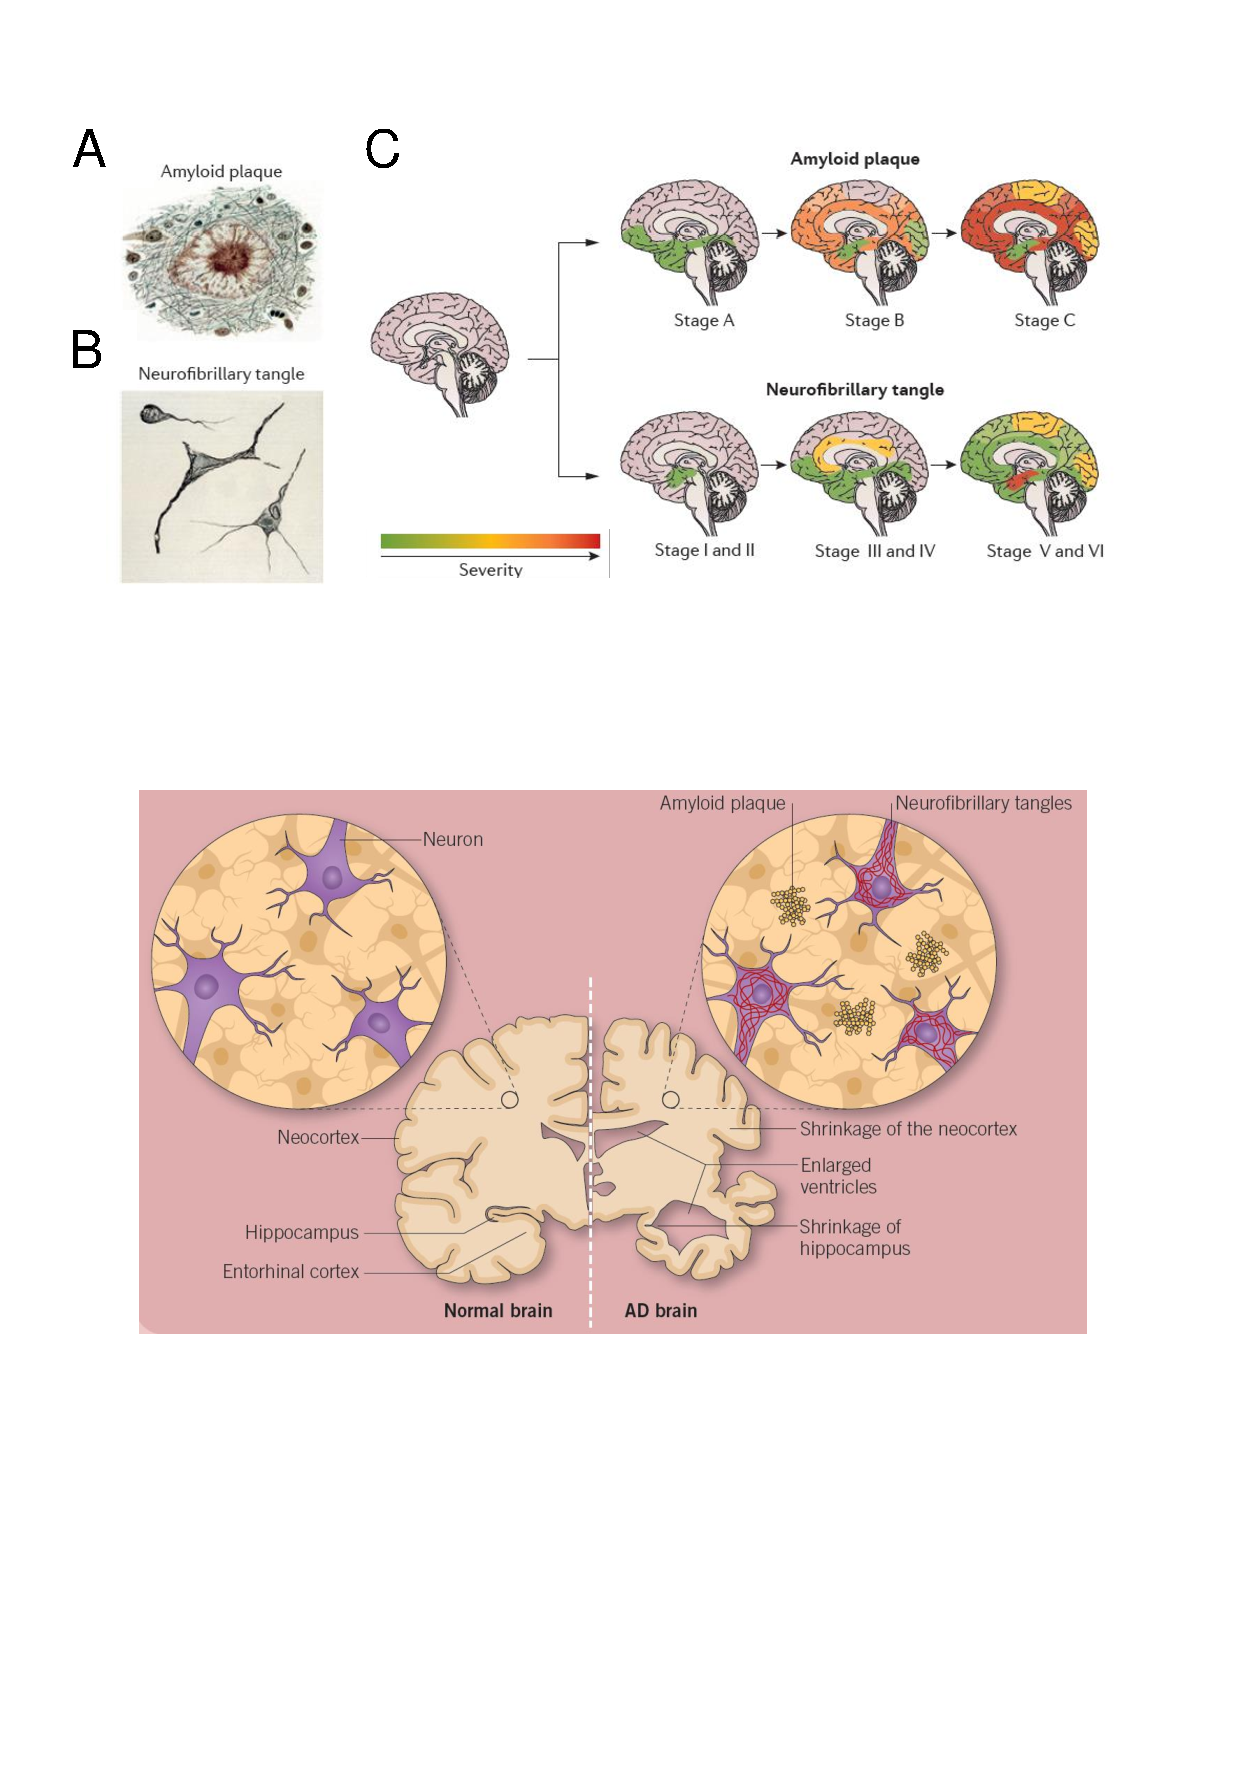
\includegraphics[page=1,trim={0 7cm 1cm 12cm},clip, scale = 0.8]{Figures/Introduction_Figures.pdf}
	\captionsetup{width=0.95\textwidth,singlelinecheck=off}
	\caption[Two key hallmarks of AD Neuropathology: amyloid plaques and neurofibrillary tangles]%
	{\textbf{Two key hallmarks of AD Neuropathology: amyloid plaques and neurofibrillary tangles}: Schema comparing a normal healthy brain and a brain with advanced AD. AD pathology is well characterised by the presence of extracellular amyloid plaques and intracellular neurofibrillary tangles, accompanied by significant neuronal loss and subsequent shrinkage of the neocortex and hippocampus. Figure is taken from Palmer (2015)\cite{AlanM.Palmer2015}
	}
	\label{fig:AD_intro}
\end{figure} 

\begin{figure}[!htp]
	\centering
	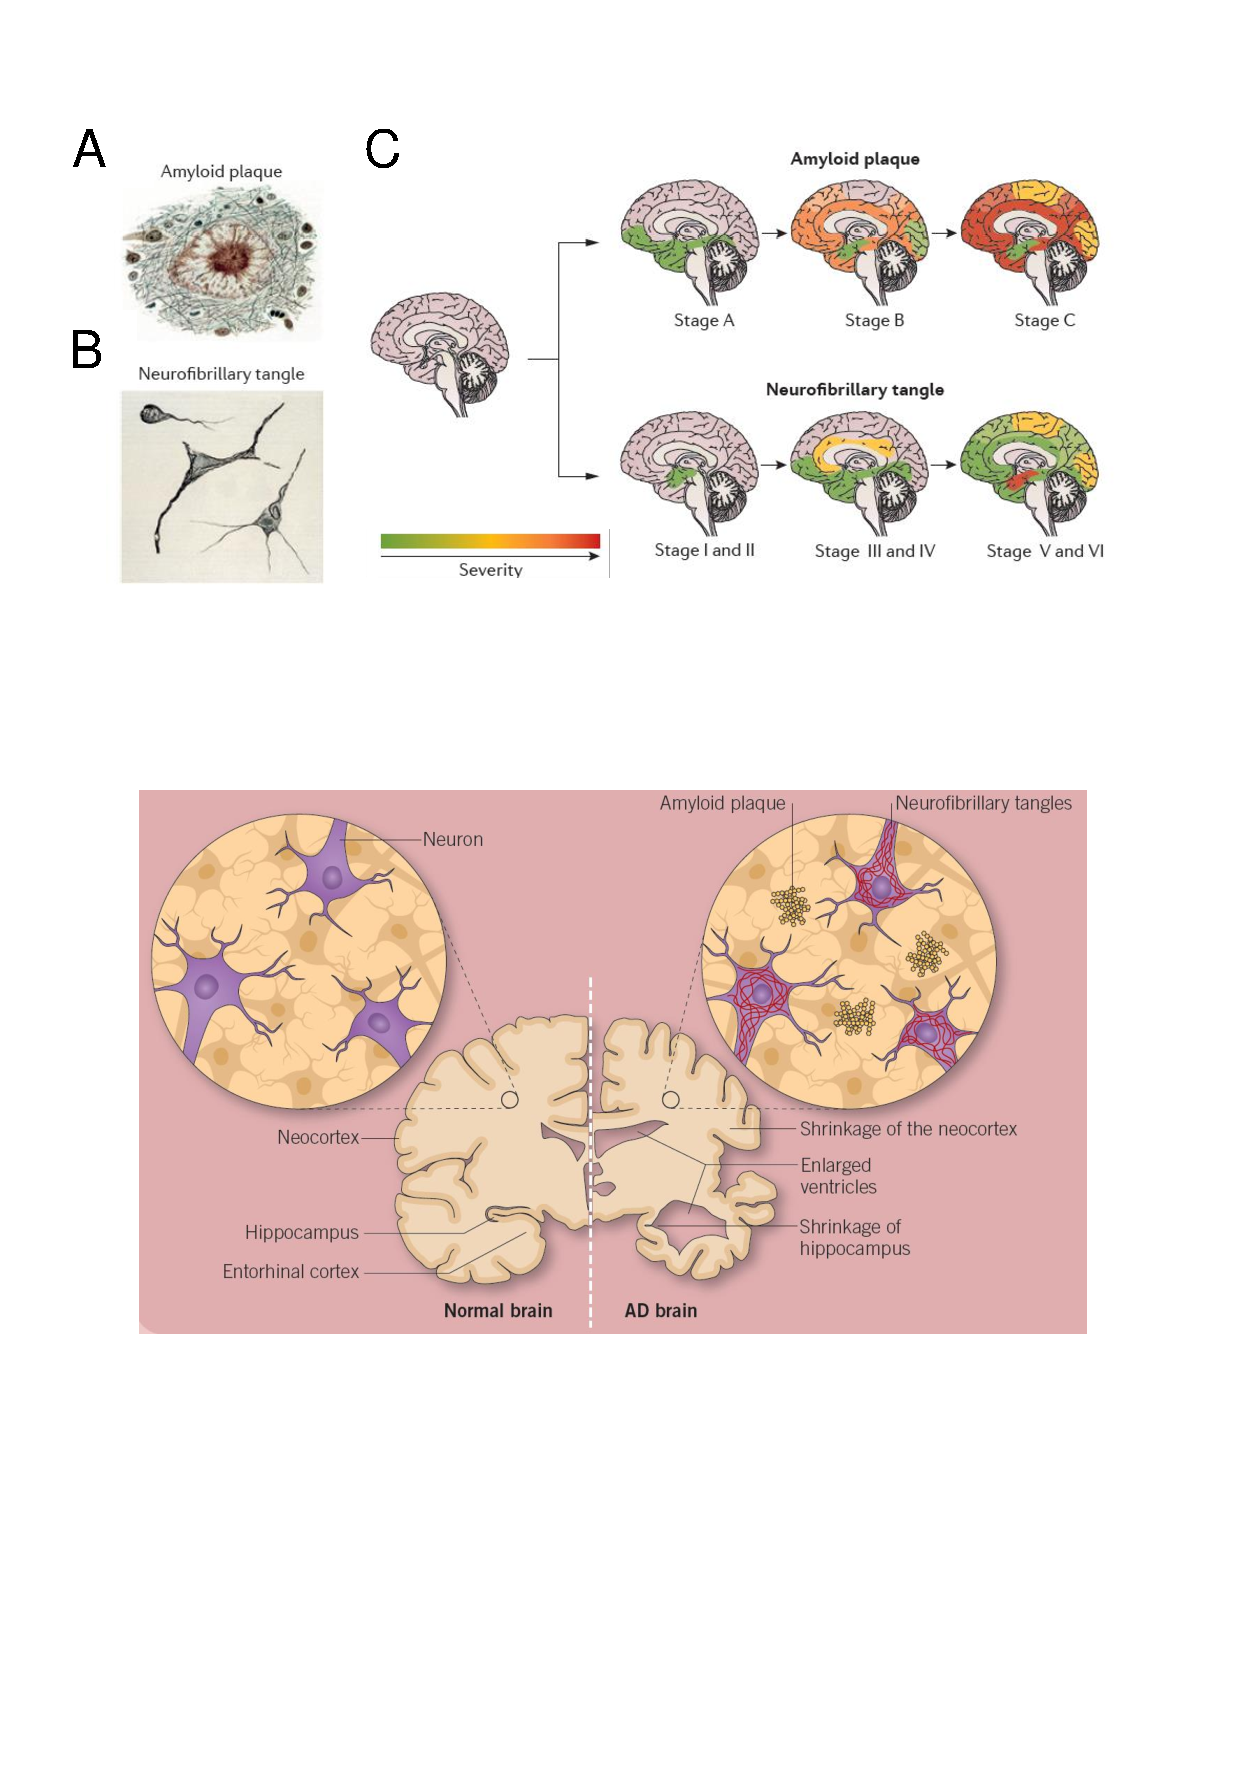
\includegraphics[page=1,trim={0 19cm 0cm 0cm},clip, scale = 0.8]{Figures/Introduction_Figures.pdf}
	\captionsetup{width=0.95\textwidth,singlelinecheck=off}
	\caption[Progression of amyloid plaques and neurofibrillary tangles with AD development]%
	{\textbf{Progression of amyloid plaques and neurofibrillary tangles with AD development}: Progression of \textbf{a)} amyloid plaques consisting of A$\beta$ measured according to Thal Phasing\cite{DR2002}, and \textbf{b)} neurofibrillary tangles composed of hyper-phosphorylated tau by Braak staging\cite{H1991}. Figure is taken from Masters et al.(2015)\cite{Masters2015}. 
		\\
		\\ 
		The deposition of A$\beta$ (Figure a) can be mapped Thal Phasing from a) the neocortex, to b) allocortical regions comprising of the entorhinal cortex and hippocampus, the striatum, and finally to iv) subcortical regions\cite{DR2002}. 
		\\
		\\
		In a similar pattern, the progressive spread of NFTs can be classified under the six stages of Braak (Figure b) from i,ii) the transentorhinal regions such as the entorhinal cortex, to the iii) hippocampus, iv) adjoining neocortex and finally to vi,v) other neocortical regions\cite{H1991}. 	
	}
	\label{fig:AD_development}
\end{figure}

\subsection{The genetics of Alzheimer's disease}
Although AD predominantly affects people aged 65 and above (referred as Late-Onset Alzheimer’s disease, LOAD\nomenclature{LOAD}{Late Onset Alzheimer's Disease}), 5\% of AD cases arise in much younger patients (Early-Onset Alzheimer’s disease, EOAD\nomenclature{EOAD}{Early Onset Alzheimer's Disease}). EOAD is normally associated with a clear familial autosomal dominant pattern of inheritance (Familial Alzheimer’s disease, FAD\nomenclature{FAD}{Familial's Alzheimer's Disease})\cite{Jarmolowicz2015}. To date, more than 160 highly-penetrant, causative mutation have been identified in EOAD, all located within three genes involved in amyloid plaque formation: \textit{APP} (amyloid precursor protein\nomenclature{APP}{Amyloid Precursor Protein}), \textit{PSEN1} and \textit{PSEN2} (presenilin 1 and 2\nomenclature{PSEN1}{Presenilin 1}\nomenclature{PSEN2}{Presenilin 2}) \cite{LM2010,Chai2007}. %While the clinical manifestations and presentation of neurological hallmarks are similar between EOAD and LOAD, patients with EOAD performed significantly worse in cognitive abilities not involved with memory (such as executive functions, language and visuoconstructional abilities)\cite{Joubert2016}.

While LOAD does not follow a Mendelian inheritance pattern, a relatively high heritability rate of 50-80\% \cite{Gatz2006} has been reported, indicating that there is still a large genetic predisposition for developing AD in later years. Indeed over recent years, genome-wide association studies (GWAS\nomenclature{GWAS}{Genome-wide association studies}) and subsequent meta-analyses \cite{Bellenguez2020,Naj2020,Kunkle2019,Jansen2019,Lambert2013,Naj2011,Hollingworth2011,Harold2009,Lambert2009,Bertram2008} have identified over 75 genetic loci associated with an increased risk of developing LOAD. These GWAS loci are typically changes (or variants) at a single DNA base-pair (single-nucleotide polymorphisms – SNPs\nomenclature{SNP}{Single Nucleotide Polymorphism}) that are found at a higher frequency in individuals with LOAD than in individuals without AD. 

The strongest genetic risk factor identified for LOAD to date is the $\epsilon$4 allele of \textit{APOE}\cite{Lambert2013}, the gene encoding for the cholesterol transporter apolipoprotein E (ApoE). This protein is a key regulator of lipid homeostasis, mediating lipid transport between astrocytes and neurons, a process critical for synaptic function and maintenance\cite{DH2001}. Harbouring one APOE$\epsilon$4 allele increases the risk of developing LOAD by 3-4x, while harbouring two $\epsilon$4 alleles increases the risk by 15x \cite{Farrer1997}; conversely, the $\epsilon$2 allele is known to confer a neuroprotective effect against AD \cite{Nagy1995,EH1994}. Although the $\epsilon$4 allele is estimated to occur in \textasciitilde 15\% of the general population, it has been observed in 40\% of patients with LOAD\cite{Farrer1997}. 

With the exception of \textit{APOE}, all the other genetics variants identified in GWAS are either common but lowly penetrant (such as those annotated to \textit{CLU, PICALM, CR1}) or highly penetrant but rare (e.g. those annotated to \textit{TREM2}) and collectively only contribute modestly to the risk of developing AD, highlighting the polygenic nature of AD (\cref{fig:AD_gwas}). While the molecular mechanisms through which these variants increase risk currently remains poorly understood, many are annotated to genes enriched in specific biological pathways, such as endocytosis, the immune system and inflammatory response, and lipid metabolism (described in \cref{aetiologyAD}). 


\begin{landscape}
	\begin{figure}[!htp]
		\centering
		\includegraphics[page=11,trim={0 17cm 0cm 1cm},clip, scale = 1.2]{Figures/Introduction_Figures.pdf}
		\captionsetup{width=1.6\textwidth,singlelinecheck=off}
		\caption[Genetic landscape of AD]%
		{\textbf{Genetic landscape of AD}: Shown are the genes implicated in AD from the causative EOAD genes (\textit{APP, PSEN1, PSEN2}) identified from early family studies, to the genes identified from GWAS studies annotated with either common but lowly penetrant or highly penetrant but rare variants. Variant penetrants, or effect size, is measured with the odds ratio (OR) with a larger odds ratio referring to a larger effect size. Variants conferring a protective effect are denoted in orange, and those with a negative effect in blue. Figure was taken from DeRojas et al. (2021)\cite{DeRojas2021}. GWAS - Genome-Wide Association Study, OR - odds ratio
		}
		\label{fig:AD_gwas}
	\end{figure}
\end{landscape}

\subsection{Molecular Mechanisms underpinning AD}
\label{aetiologyAD}
Despite the fact that AD neuropathology has been well described, the exact biological mechanisms driving AD onset and pathogenesis are still widely unknown. To date, there are two key hypotheses proposed for the progression of AD: i) the amyloid cascade hypothesis, ii) the tau tangle hypothesis. Results from GWAS, however, implicate other pathways that could be involved including a dysfunctional immune response, lipid metabolism, endocytosis, and cell-adhesion molecule (CAM) pathways for synaptic signalling.  

\boldheader{Amyloid cascade hypothesis} 
The amyloid cascade hypothesis posits that the extracellular accumulation of A$\beta$ is the key driver of AD pathogenesis, which initiates a pathological cascade of NFT, cell loss, vascular damage \cite{Hardy1992}. A$\beta$ is comprised of short peptides (39-43 amino acids) \cite{J1987} produced from the amyloidogenic cleavage of APP (a transmembrane protein involved in synapse formation and stability) by $\beta$-secretase (BACE - β-site APP-cleaving enzyme 1\nomenclature{BACE}{Beta-secretase}) and $\gamma$-secretase (a complex protein consisting of PSEN1 and PSEN2) (\cref{fig:APP_Processing}). Due to cleavage at various sites, $\gamma$-secretase produces A$\beta$ of varying lengths, with 90\% secreted as A$\beta$\textsubscript{40} and the remaining 10\% as A$\beta$\textsubscript{42}\cite{Asami-Odaka1995}.

\vspace{1cm}
\begin{figure}[!htp]
	\centering
	\includegraphics[page=2,trim={0 9cm 0cm 15cm},clip, scale = 0.8]{Figures/Introduction_Figures.pdf}
	\captionsetup{width=0.95\textwidth,singlelinecheck=off}
	\caption[Sequential cleavage of APP into A$\beta$ by $\beta$-secretase and $\gamma$ secretase]%
	{\textbf{Sequential cleavage of APP into A$\beta$ by $\beta$-secretase and $\gamma$ secretase}: Schema depicting sequential cleavage of APP, a transmembrane protein, either through the \textbf{a)} non-amyloidogenic pathway or \textbf{b)} the amyloidogenic pathway.
		\\
		\\
		In the non-amyloidogenic pathway, APP is cleaved by ADAM protein family (primarily, ADAM10, also known as $\alpha$-secretases) followed by $\beta$-secretase. Conversely in the amyloidogenic pathway, APP is sequentially cleaved by by $\beta$-secretase and $\gamma$-secretase, which can produce A$\beta$ of varying lengths. Monomeric A$\beta$ molecules, particularly, A$\beta$42, have increased propensity to oligomerise and aggregate to form the fibrils and plaques that are characteristic of AD. Figure is taken from Acker et. al (2019)\cite{Acker2019}. 
	}
	\label{fig:APP_Processing}
\end{figure}

In AD, the processing of APP is altered with the vast majority of causative \textit{APP}, \textit{PSEN1} and \textit{PSEN2} mutations favouring the production of the longer and more self-aggregating A$\beta$42 \cite{Li2019,D1996,JT1993}, thereby promoting the formation of insoluble fibrils and plaques\cite{JT1993}. 

%https://www.nature.com/articles/nrn2620

%Although interestingly, the neuroprotective ApoE$\epsilon$2 allele while associated with intact cognition is also associated with AD pathology in the oldest old population\cite{DJ2009}, suggesting that an A$\beta$-independent mechanism may be at play.   

%"TREM2 mediated phagocytosis is critical for Aβ and neuronal debris clearance in AD (Kleinberger et al., 2014; Xiang et al., 2016; Yeh et al., 2016). Specifically, TREM2 expression is important for microglia to physically associate with Aβ plaques (Ulrich et al., 2014; Wang et al., 2016; Yuan et al., 2016; Jay et al., 2015, 2017a,b)." 

%"CD33 is elevated in the AD brain in microglia and infiltrating macrophages and is thought to modulate microglial activation and Aβ clearance (Griciuc et al., 2013; Walker et al., 2015).  In fact, knock-out of CD33 in AD mouse models results in reduced Aβ plaque burden (Griciuc et al., 2013). 

\boldheader{Tau tangle hypothesis} 
%https://pubmed.ncbi.nlm.nih.gov/33848474/
The tau hypothesis posits that the phosphorylation and aggregation of tau to form NFTs are the primary drivers of AD\cite{KS1986}, which is also the defining feature of more than 20 other neurodegenerative disorders known collectively as tauopathies\cite{Orr2017}. Tau, encoded by the \textit{MAPT} gene, is a microtubule-associated protein involved in microtubule maintenance and stability. 

Recent studies suggests that hyper-phosphorylated tau dissociates from microtubules and aggregates into filaments\cite{Grundke-Iqbal1986,Grundke-Iqbal1986a} (components of NFTs) that disrupt axonal transport and signal transmission, ultimately resulting in synpatic degeneration and loss\cite{Coomans2021} (\cref{fig:tau_hypothesis}).  Tau mutations associated with frontotemporal dementia and Parkinsonism (FTDP) \nomenclature{FTDP}{Frontotemporal dementia and parkinsonism} are found to induce conformational changes that increase the affinity for phosphorylation\cite{Alonso2004}. While no causative mutations in \textit{MAPT} have been identified in AD, the severity of NFTs has shown to correlate better with cognitive decline and disease progression than amyloid plaques \cite{Serrano-Pozo2016,Giannakopoulos2003,PV1992} with its spread traced through Braak staging \cite{H1991} (\cref{fig:AD_development}\textbf{b}).

%Regional variation in MAPT mRNA and protein expression was observed with a 2-fold higher level in the neocortex than the cerebellum, any may explain regional vulnerability of brain regions to tau pathology\cite{Trabzuni2012}. 

\boldheader{Endocytosis} 
Endocytic processing (i.e. the internalisation of substrates into the cell) is directly implicated in AD due to distinct cellular localisation of secretases involved in the amyloidogenic processing of APP\cite{Acker2019}. Contrary to the non-amyloidogenic pathway that predominantly occurs at the plasma membrane\cite{Sisodia1992}, amyloidogenic processing of APP takes place in the endosome and is spatially regulated: BACE1 and PSEN1/$\gamma$ complex are localised at the plasma membrane and thus must first undergo endocytosis before assemblage with PSEN2/$\gamma$ secretase at the endosome (\cref{fig:APP_Trafficking}). Increasing evidence suggest that regulation of this endocytic pathway is altered in AD, creating an intracellular pool of A$\beta$ peptides \cite{Peric2015}; pathological significance of these intraneuronal peptides have been corroborated in AD mouse models with their appearance coinciding with cognitive deterioration in AD mouse models \cite{Tomiyama2010,Knobloch2007,Billings2005} and with stronger association to neuronal loss than A$\beta$ plaques\cite{Christensen2008}. Indeed, several risk genes emerging from recent GWAS are directly involved in endocytic regulation of APP processing, including: i) \textit{Bin1}, ii) \textit{Picalm}, and iii) \textit{Sorl1}, which encodes for SORLA (encoded by \textit{SORL1}), an APP-binding receptor involved in APP trafficking away from the late endosome for amyloidogenic processing and facilitating A$\beta$ degradation in lysosome \cite{Schmidt2016,Dumanis2015}.   

\vspace{1cm}
\begin{figure}[!ht]
	\centering
	\includegraphics[page=13,trim={0 14cm 0cm 2cm},clip, scale = 0.7]{Figures/Introduction_Figures.pdf}
	\captionsetup{width=0.95\textwidth,singlelinecheck=off}
	\caption[Tau hypothesis in AD]%
	{\textbf{Tau dissociation from microtubules and aggregation into NFTs}: Schema depicting a \textbf{a)} healthy and \textbf{b)} diseased neuron, with hyper-phosphorylated tau (orange spikes) detaching from microtubules. This results in microtubule dissociation and subsequent interrupted neuronal growth and function, essential for synaptic transmission. Figure is taken from Brunden et al. (2009)\cite{Brunden2009}
	}
	\label{fig:tau_hypothesis}
\end{figure}	


\begin{figure}[!htp]
	\centering
	\includegraphics[page=6,trim={0 8cm 0cm 0cm},clip, scale = 0.8]{Figures/Introduction_Figures.pdf}
	\captionsetup{width=0.95\textwidth,singlelinecheck=off}
	\caption[Spatial regulation of APP trafficking and processing]%
	{\textbf{Spatial regulation of APP processing}: Schema depicting APP trafficking and processing through the non-amyloidogenic (\cref{fig:APP_Processing}\textbf{a}), which predominantly occurs at the plasma membrane (boxed green), and amyloidogenic pathway (\cref{fig:APP_Processing}\textbf{b}), which preferentially occurs in the endosome (boxed red). APP processing through the amyloidogenic pathway is spatially regulated by the localisation and distinct internalisation of assembled PSEN1/$\gamma$ complex and BACE1 at the plasma membrane (boxed purple) and PSEN2/$\gamma$ in the endosome. Figure is adapted from Acker et. al (2019)\cite{Acker2019}  
	}
	\label{fig:APP_Trafficking}
\end{figure}



\boldheader{Immune Response}
Profound neuroinflammation, an inflammatory response within the CNS primarily orchestrated by the activation of microglia (microgliosis) and astrocytes (astrogliosis) with heightened release of cytokines, has been widely implicated in AD development pathology \cite{Cisbani2021,Griciuc2021}. While the role of the immune response is poorly understood in AD, it is widely accepted that an imbalance of the innate immune response is at play\cite{Frost2019} (\cref{fig:microglia_AD}\textbf{a}). Reactive microglia has been found surrounding amyloid plaques\cite{PL1987}, suggesting that plaque-associated microglia have a compromised phagocytic ability to remove A$\beta$\cite{Mawuenyega2010} - a complex process that involves recognition of toxic species (in this case, detrimental protein aggregates) by receptors, such as TREM2, CD33 and CR1, which are all GWAS AD risk genes. (\cref{fig:microglia_AD}\textbf{b}). Furthermore, reactive microglia can also release pro-inflammatory neurotoxic cytokines that can trigger neuronal apoptosis\cite{Qin2002,Wang2015b} and upregulate β-secretase\cite{Chen2012}, resulting in enhanced A$\beta$ propagation (\cref{fig:microglia_AD}\textbf{b}).  

Multiple recent transcriptomic profiling studies of single cells in AD human post-mortem brain tissue\cite{Mathys2019,Nott2019,Thrupp2020,Olah2020,Leng2021,Young2021} and AD mouse models\cite{Keren-Shaul2017,Mathys2017} have revealed subpopulations of microglia and astrocytes that have an altered molecular expression signature associated with disease progression. Proliferation of these distinct AD-associated microglial cells were accompanied with release of pro-inflammatory cytokines and increased expression of interferon-response genes\cite{Mathys2017}. Similar microglial cell states (termed disease-associated microglia - DAM\cite{Keren-Shaul2017}, and activated response microglia - ARM\cite{Frigerio2019}) have been also characterised in mouse models with upregulated expression in innate immune response and interferon pathways. Moreover, these AD-associated microglia subpopulations were enriched with altered expressions of \textit{Trem2} and \textit{Cd33} \cite{Mathys2019,Frigerio2019}. A subset of AD-associated astrocytes, likely to represent reactive astrocytes, has also been characterised with upregulated expression of \textit{Gfap} and \textit{Cd44}, and downregulation of genes associated with homeostasis\cite{Leng2021}. Notably, the largest proteomic study to date identified that the protein co-expression module most robustly associated with AD and FTD was also associated in astrocyte- and microglial-associated proteins, and was significantly enriched in AD GWAS genes and protective markers of anti-inflammatory disease-associated microglia \cite{Johnson2020}.    

%Role of adaptive immune response with recent identification of a subpopulation of immune cells, CD8+ T effector memory CD45RA+ (TEMRA), associated with AD pathology and exhibited stronger antigenic stimulation (increase in cytokine signalling) \cite{Gate2020}. In addition to the stronger-associated AD risk variants, previous studies have identified additional rare coding variants in genes involved in the immune response\cite{R2017,Bis2018} and transcriptional regulation\cite{Bis2018}.

\begin{figure}[!htp]
	\centering
	\includegraphics[page=8,trim={0 8cm 0cm 0cm},clip, scale = 0.8]{Figures/Introduction_Figures.pdf}
	\captionsetup{width=0.95\textwidth,singlelinecheck=off}
	\caption[Role of microglia in AD development and pathology]%
	{\textbf{Role of microglia in AD development and pathology}: A simplified schema illustrating the \textbf{a)} multifaceted roles of microglia in AD, ranging from a protective to a detrimental role by the respective secretion of anti- and pro-inflammatory cytokines, and \textbf{b)} Microglia's dual response to A$\beta$ plaques, either through A$\beta$ clearance or release of pro-inflammatory cytokines. Recent emergence of single RNA-sequencing studies have revealed significant heterogeneity in microglia isolated from AD post-mortem brain tissues, highlighting the complex role that microglia plays in AD development and pathology. Under physiological conditions, the microglia is ramified. PRR - Pattern recognition receptors, such as TREM2 and CD33, are found on the cell surface of microglia and are involved in recognising toxic species for phagocytosis. Both figures are adapted from Leng et al. (2021)\cite{Leng2021a}  
	}
	\label{fig:microglia_AD}
\end{figure}


\boldheader{Lipid Metabolism}
\label{intro_lipid}
Identification of \textit{Apoe} $\epsilon$4 variant as the most robustly LOAD-associated genetic variant established a link between lipid metabolism and AD. Increasing evidence further postulates that A$\beta$ clearance is regulated in an APOE isoform-dependent manner\cite{Castellano2011} with APOE4 having low binding affinity to A$\beta$ and thus, being the least efficient at A$\beta$ clearance\cite{RM2012} - carriers of $\epsilon$4 allele have more pervasive amyloid plaques than non-carriers\cite{DE1993,E2009}. APOE lipidation status, mediated by ABCA1\cite{R2010}, has also been reported to impact A$\beta$ aggregation, with APOE4 being poorly lipidated compared to APOE2 and APOE3, resulting in increased propensity to aggregate\cite{DM2006}. 

More broadly, lipid metabolism and homeostasis are linked to AD development in that APP, $\beta$- and $\gamma$-secretase are transmembrane proteins (\cref{fig:APP_Trafficking}); lipid membrane constitution and organisation would therefore have an impact on the APP trafficking and secretase activities \cite{DiPaolo2011}. \textit{ABCA7}, by regulating the lipid composition at bilayer, can indirectly influence the activity and expression of $\beta$-secretase \cite{Sierksma2020,Sakae2016}.  

%CLU

\boldheader{Interplay of multiple molecular pathways}
While the two key hypothesis of amyloid plaque formation and tau aggregation are widely supported, identification of AD-associated genes, enriched in multiple pathways, highlight the complexity and multifacetted nature of the disease. As described above, genetic studies of AD strongly implicate pathways centred on abnormal A$\beta$ trafficking, processing, and clearance. Recent studies have also revealed interplay between pathways, with APOE4-expressing microglia exhibiting less active transcriptional response and reduced uptake A$\beta$ than APOE3-expressing microglia, which is further exacerbated by Trem2 deficiency\cite{Fitz2021}.  


%https://science.sciencemag.org/content/370/6512/61?rss=1


%\boldheader{Synpatic signalling} 

\clearpage
\subsection{Modelling AD: Transgenic Mouse Models}
While profiling human post-mortem brain tissues remains the gold standard for studying AD pathogenesis, there are various confounding secondary factors (e.g. environmental exposures such as diet, medication) and technical difficulties (e.g. agonal state and post-mortem interval impacting RNA quality) to consider. In comparison, mouse models of disease can be tightly controlled (i.e. for genotype, living conditions, their age and pathological status) to enable analyses into the progression of pathology in disease-relevant cell-types.  

To study the different aspects of pathology, a number of transgenic AD mouse models have been developed with mutations that either result in amyloidopathy (formation of A$\beta$ plaques) or tauopathy (NFT) (\cref{tab:mouse_models}). Amyloidopathy is typically developed through the insertion and overexpression of human \textit{APP}, either alone or in combination with \textit{PSEN1}, whereas tauopathy is recapitulated by overexpressing human \textit{MAPT} with FTD-associated mutations (given no causative \textit{MAPT} mutations have been identified in AD). The insertion of transgenes, however, have been found to disrupt endogenous mouse genes that may significantly contribute to the neurodegenerative phenotype observed in these mice. 

It is also important to note that there are currently no mouse model that encapsulates all the defining features of AD and one of the major criticisms of current AD mouse models relates to how representative they are of sporadic, late-onset AD. There have been recent efforts to generate mouse models that more closely resemble LOAD with the incorporation of AD-associated variants, such as $\epsilon$ variant of \textit{APOE} and R47H \textit{Trem2} variant \cite{apoe4trem2_mousemodel,Lewandowski2020}, however these are not widely used.

Nonetheless, current mouse models act as a valuable reductionist tool to dissect the processes that drive the onset and study the pathology of AD pathology, identify biomarkers and validate novel targets\cite{Hall2012}. In my thesis, I utilise the rTg4510 mouse model to profile progressive changes in splicing and isoform regulation associated with development of tau pathology. More details about this model are provided in \cref{ch: general methodology}. 


\begin{table}[htp]
	\centering
	\setlength\tabcolsep{3.5pt}
	\captionsetup{width=1\textwidth}
	\caption[Representative AD Mouse Models]%
	{\textbf{Representative AD mouse models}. Tabulated is a list of the most widely used AD mouse models developed from overexpression of one or more genes associated with FAD. Table is adapted from Hall et al. (2012) \cite{Hall2012} and is by no means comprehensive. mo - months}
	\label{tab:mouse_models}
	\begin{threeparttable}
		\begin{tabular}{@{}lllcccc@{}}
			\toprule
			\multicolumn{2}{c}{Mouse Models} &
			\multicolumn{1}{c}{Mutations} &
			\begin{tabular}[c]{@{}c@{}}Plaques\\  (mo)\end{tabular} &
			\begin{tabular}[c]{@{}c@{}}Tangles\\   (mo)\end{tabular} &
			\begin{tabular}[c]{@{}c@{}}Neuronal \\ Loss (mo)\end{tabular} &
			\begin{tabular}[c]{@{}c@{}}Cognitive \\ Deficit (mo)\end{tabular} \\ \midrule
			\multirow{4}{*}{hAPP}     & PDAPP                 & Ind\tnote{b}                        & 6  & x  & x     & 6                \\
			& Tg2576                & Swe\tnote{a}             & 11 & x  & x     & \textgreater{}12 \\
			& J20                   & Swe\tnote{a}, Ind\tnote{b} & 6  & x  & x     & 4                \\
			& APP23                 & Swe\tnote{a}               & 6  & x  & 14-18 & 3                \\
			\multirow{3}{*}{hAPP/PS1} & PS/APP & Swe\tnote{a}, M146L\tnote{e}                 & 6  & x  & 22    & 3                \\
			& APP/PS1         & Swe\tnote{a}, PSEN1dE9              & 6  & x  & x     & 6                \\
			& 5xFAD                 & Swe\tnote{a}, Lon\tnote{a}, Flo\tnote{c}, M146L\tnote{e}, L28V\tnote{e} & 2  & x  & 9     & 4                \\
			\multirow{4}{*}{hTau}     & hTau.P301S            & MAPT P301S                 & x  & 4  & 3     & 3                \\
			& 3xTg                  & Swe\tnote{a}, MAPT P301L, M146V     & 6  & 12 & -    & 4                \\
			& rTg4510               & MAPT P301L                 & x  & 4  & 6     & 3                \\
			& htau                  & Wildtype                   & x  & 9  & 10    & 6                \\ \cmidrule(l){1-7} 
		\end{tabular}
		\begin{tablenotes}
			\footnotesize
			\item[a] Swedish APP mutation K670N/M671L
			\item[b] Indiana APP mutation V717F
			\item[c] London APP mutation V717I
			\item[d] Florida APP mutation I716V 
			\item[e] Human PSEN1 mutations 
		\end{tablenotes}
	\end{threeparttable}
\end{table}


%rtg4510: https://journals.plos.org/plosone/article?id=10.1371/journal.pone.0106050


\clearpage
\section{Transciptional dysregulation in AD}

The vast majority of variants associated with LOAD are annotated to non-coding regulatory regions of the genome, being enriched in open chromatin regions that promote transcription such as enhancers\cite{Kikuchi2019} (short DNA sequences containing specific motifs for binding of transcription factors). Recent single cell studies have further demonstrated that AD-associated non-coding SNPs are enriched in microglia enhancers with cell-type specific regulation of gene expression\cite{Tansey2018,Nott2019,Young2021,Novikova2021}, suggesting that AD-associated risk variants mediate disease associations through gene regulation. 

Efforts to better understand the expression changes in AD by profiling the complete set of expressed RNA transcripts (hereby referred as transcriptome) in AD mouse models and post-mortem brain tissues have been essential in revealing insights into the molecular mechanisms that underlie AD risk variants. A number of studies have identified widespread gene differences in transgenic mice harbouring AD-associated mutations and affected post-mortem brain regions (reviewed in XXX). Recent works in our group have similarly identified robust changes in gene expression associated with tau pathology development in rTg4510, with these genes found to be enriched in pathways previously implicated in AD pathology\cite{Castanho2020}. In addition to expression changes observed at the gene level, there is increasing evidence for the role of altered splicing regulation (more detail is provided in \cref{intro:AD_alteredsplicing}). These AD-associated splicing changes are also enriched in genes involved in pathways previously implicated such as the immune response and synaptic transmission, adding to the layer of complexity underlying AD pathogenesis. 

%lead variant of \textit{BIN1} (rs6733839C>T) was preferentially located in OCR of microglia and predicted to increase binding affinity for MEF2C transcription factor, subsequently increasing \textit{BIN1} expression \cite{Young2021}. Deletion of microglia-specific enhancer reduced BIN1 expression in microglia, but not in neurons an astrocytes\cite{Nott2019}
%Transcriptomic landscape profiling of disease-relevant tissues, in taking a snapshot of the present state of the cells, is key to elucidating the functional relationship between the genetic variants identified from GWAS and the molecular mechanisms that drive disease development and pathology in a time- and tissue-dependent manner \cite{Verheijen2018}.  %https://pubmed.ncbi.nlm.nih.gov/31626773/
%Between all the regulatory mechanisms influencing gene expression, there is a growing recognition that non-coding variants effects are mediated through alternative splicing in neuropsychiatric diseases, including schzizophrenia and autism
%https://pubmed.ncbi.nlm.nih.gov/31451803/


\subsection{Alternative Splicing}
Alternative splicing is a transcriptional regulatory mechanism that produces distinct transcripts (isoforms) from a single gene, which are potentially translated to different protein isoforms with unique, and potentially, antagonistic functions\cite{Wang2008}. It is a widespread phenomenon with over 95\% of human genes estimated to be influenced \cite{Pan2008}, and is most prevalent in the brain\cite{Yeo2004}, where it impacts upon neuronal development and maintenance\cite{Pan2008, Mazin2014, Raj2015}. There is a growing recognition of the key role of aberrant mis-splicing in neurodegenerative diseases \cite{Gandal2018,RL2019}, including schizophrenia and autism. 

\boldheader{Mechanism}
Splicing involves the removal of non-coding sequences (introns) from mRNA precursors and the ligation of coding sequences (exons), resulting in isoforms with different exonic structures (\cref{fig:AS_events}). This relies on the concerted and regulated assembly of the spliceosome (a multimegaton, dynamic ribonucleoprotein complex) by its recognition and stepwise-binding to sequence elements within the pre-mRNA (cis-elements), and a group of regulating splicing factor proteins (trans-elements) (\cref{fig:AS_mechanism}). Recent studies suggest that this process occurs co-transcriptionally, such that the intron can be identified and removed as soon as it is synthesised by the RNA polymerase. 
%There are two types of spliceosome - major and minor - both of which involve the activity of five uridine-rich small nuclear ribonucleoproteins (snRNP\nomenclature{snRNPs}{Small Nuclear Ribonucleoproteins}) and numerous non-snRNP proteins\cite{Will2011}. Using a similar mechanism but composed of different snRNPs, the minor spliceosome removes less than 1\% (0.4\%) of introns\cite{Turunen2013} and is thus referred to as "U12-dependent non-canonical splicing", as opposed to "U2-dependent canonical splicing" with major spliceosome.

Correct splicing first requires recognition of short sequence motifs upstream (5' splice site, 5'SS\nomenclature{5'SS}{5' Splice Site}, donor site) and downstream (3' splice site, 3'SS\nomenclature{3'SS}{3' Splice Site}, acceptor site) of the intron/exon boundary, followed by sequential assembly of the spliceosome components and intron excision\cite{Herzel2017}. The 5'SS is typically defined by a conserved 9-nucleotide sequence with a GU(T) dinucleotide, and the 3'SS by a polypyrimidine tract (PPT\nomenclature{PPT}{Polypyrimidine Tract}) followed by a conserved AG dinucleotide \cite{Will2011}. Almost all introns in human and mouse are flanked by the GT-AG splice site dinucleotides\cite{Sheth2006} (termed splice junctions), with other dinucleotide variations known to exist in very minute proportions: GC-AG and AT-AC comprises \textasciitilde0.9 and \textasciitilde0.09\% of human splice sites\cite{Parada2014}. An increasing number of disease are linked to aberrant alternative splicing by pathogenic variants by interfering cis-acting elements (5'SS and 3'SS, resulting in exon skipping, exon inclusion, exon extension or exonic splice gain; intron resulting in intron gain) and action of trans-acting protein splicing factors.

%Alternative splicing is highly-regulated in a temporal and cell-specific manner by the binding and fin-tune balance of trans-acting factors to cis-acting elements. The sequence of these cis-acting elements within the exon (exonic splicing - ES) or intron (intronic splicing - IS) determines the binding affinity of the trans-acting factors to either enhance or suppress splicing. RNA structure also plays a role in blocking or allowing trans-acting factors to bind, and transcription factor assemblage through distal interactions. 
%Trans-acting factors include RNA-binding proteins such as SR protein (serine and arginine-rich proteins), heterogeneous nuclear ribonucleoproteins (hnRNPs, and other tissue-specific proteins and complementary microRNA (miRNAs); Cis-elements include exonic splicing enhancers and silencers ( ESEs, ESSs), intronic splicing enhancers and silencers (ISEs, ISSs). Localisation and function of trans-factors are further regulated by post-translational modifications, adding to the layer of complexity through activation/suppression from other proteins involves post-translational modifications i.e. kinases and phosphatases. 


\vspace{1cm}
\begin{figure}[!htp]
	\centering
	\includegraphics[page=9,trim={0 16.5cm 0cm 0},clip, scale = 0.7]{Figures/Introduction_Figures.pdf}
	\captionsetup{width=0.95\textwidth,singlelinecheck=off}
	\caption[Alternative Splicing Events]%
	{\textbf{Alternative Splicing Events}: Splicing involves removal of introns and ligation of exons either constitutively or alternatively to generate isoforms with different exonic structure: an exon can be entirely skipped (orange exon in SE) or two exons that are not spliced together (orange and blue exon in MX), an intronic sequence can be retained (light orange in IR), a different 5'SS or 3'SS can be used resulting in a novel splice junction (A5', A3'), and the usage of different first and last exons which can result in an alternative promoter and termination.  
	}
	\label{fig:AS_events}
\end{figure}


\begin{figure}[!htp]
	\centering
	\includegraphics[page=3,trim={0 14cm 8cm 2cm},clip, scale = 0.8]{Figures/Introduction_Figures.pdf}
	\captionsetup{width=0.95\textwidth,singlelinecheck=off}
	\caption[Splicing Mechanism: spliceosome assembly on nascent RNA]%
	{\textbf{Intron removal is catalysed by the assembly and complex rearrangement of spliceosome. a)}:  Consensus sequence of splice sites that demarcate the intron/exon boundary and are essential for recruitment of spliceosomal snRNPs. \textbf{b)} Co-transcriptional assembly of spliceosome with stepwise interaction of spliceosomal snRNPs, with the formation of 
		\begin{enumerate}
			\item E (Early) commitment complex with the identification and binding of U1 snRNP to the 5'SS and branchpoint binding protein (BPP\nomenclature{BPP}{Branchpoinnt Binding Protein} to BPS 
			\item A (Assembly) catalytically-active complex with association of U2 snRNP to the branch site following the dissociation of BPP. The "A" here denotes to the adenosine of BPS
			\item B pre-catalytic spliceosome complex with recruitment of U4,U5 and U6 snRNPs
			\item B pre-catalytic spliceosome complex after major conformational rearrangements within the spliceosome (RNA-protein and RNA-RNA interactions) followed by the release of U1 and U4 snRNP to expose the adenosine from BP to the 5'SS 
			\item B* catalytically-active complex with nucleophilic attack of adenosine on 5'SS (first step of transesterification) 
			\item C catalytically-active complex with further conformational changes in the U2 snRNA to C* complex, with nucleophilic attack of the 5'SS to 3'SS (second step of trans-esterification) 
			\item P (Post-spliceosome complex). The mRNA product is then released from remaining spliceosome (ILS), now bound to the intron lariat. The snRNPs can then disassociate and be recycled for next cycle of splicing.
			\\
		\end{enumerate} 
		Intron excision is primarily executed by two trans esterification reactions.	BPS - Branch point sequence, CTD - carboxyl-terminal domain, ILS - Intron lariat spliceosome, PAS - poly(A) site, SS - Splice site, TSS - Transcription start site,TTS - Transcription termination site. Figure is taken from Herzel et al. 2017\cite{Herzel2017}.
	}
	\label{fig:AS_mechanism}
\end{figure}

%\boldheader{Other regulatory mechanisms}
%Of note, splicing is only one of the main ways of gene regulation;pre-transcriptional regulation involving chemical modifications of DNA nucleotides (epigenetics), transcriptional regulation involving the binding of transcription factors and post-transcriptional regulation involving the processing of mRNA transcripts. Splicing works with these mechanisms together (?). 
%AS further regulates gene expression through various mechanisms: non-sense mediated decay, miRNA-mediated mRNA degradation, altered translational efficiency of isoforms. In contrast, alternative polyadenylation regulates RNA transportation, localization, stability, and translation by generating splice isoforms with different cleavage sites. Nonsense mediated decay (NMD) \nomenclature{NMD}{Nonsense Mediated Decay} products are alternatively spliced isoforms that are not translated into proteins, by containing an early stop codon. A premature termination-translation codon highly supportive of NMD is defined by a stop codon within at least 50-55 base pairs upstream of splice junctions.  up to 70\% containing multiple polyadenylation sites and 60\% with two or more promoters from alternative transcription start sites \cite{Carninci2006}. In addition to above five common categories, many other complex types, such as alternative position, i.e., alternative 3' and 5' site (Wang and Brendel, 2006), AS and transcriptional initiation (ASTI) (Nagasaki et al., 2006) alternative first exons (Chen et al., 2007), and composite patterns (Wang and Rio, 2018), can occur.
%Introduction of variable segments within otherwise identical mRNAs, with 80% of this variability observed within open reading frames (ORFs), subsequently contributing significantly to proteome diversity, and 20% falling within untranslated regions that regulates cis-binding effects. (G. S. Wang & Cooper, 2007) Subsequently, influencing mRNA stability, translation efficiency (including miRNA binding sites), and mRNA localisation. One-third of alternative splicing events introduce premature termination codons (PTCs), which cause mRNA degradation by nonsense-mediated decay (NMD) (Lewis, Green, & Brenner, 2003). Therefore, alternative splicing regulates temporal and spatial expression of functionally diverse isoforms, on–off regulation by NMD, or other post-transcriptional regulatory responses; also for cell identity, whereby number of tissue-specific isoforms highest in the brain. 
%Still high error rate accuracy of nanopore "The raw accuracy of nanopore 1D cDNA sequencing is ~85–87%36–38, although accuracy can change depending on iterations of the technology and library preparation methods37" \cite{Tang2020}

\newpage
\subsection{Altered splicing in AD}
\label{intro:AD_alteredsplicing}
Dysregulation of splicing can have significant functional consequences in driving or contributing to disease progression and susceptibility, by disrupting protein isoform function (loss-of-function or gain-of-function) or generating an imbalanced isoform ratio (i.e. a change in relative isoform expression). Studies on the role of alternative splicing in AD have largely focused on specific FAD genes, such as \textit{PSEN1, APP and MAPT}; e.g. a mutation in intron 4 of PSEN1 produces aberrantly-spliced truncated PSEN1 isoforms that were found to increase A$\beta$42 \textit{in vitro}\cite{DeJonghe1999}. Perhaps more well known is the altered splicing of MAPT whereby exclusion or inclusion of exon 10 (E10) generate isoforms with either 3 (3R tau, E10-) or 4 (4R tau, E10+) microtubule-binding repeat domains, with the latter having a greater interaction with microtubules. Over 50 tauopathy-associated intronic mutations were found clustered around the 5'splice site of exon 10 in favouring inclusion of exon 10 \cite{DSouza1999, Ghetti2015}, resulting in increased production of 4R tau and imbalanced 4R/3R ratio that contribute to tau aggregation \cite{Adams2010} - mimicking this imbalanced ratio in a tauopathy mouse model induced more seizures, and more phosphorylated,self-aggregating tau \cite{Schoch2016}.  
%tau-isoform mediated neurodegeneration   
% efforts to better understand gene expression changes in AD by sequencing transcriptome of affected brain regions


%(Trabzuni et al 2012)(Rockentein et al 1995)(Buee et al 2000)(Valenca et al. 2016) studies on AS

Notably, multiple spliceosomal components were found to co-aggregate with tau in post-mortem AD brain tissues\cite{Bai2013}, indicating that there is a global change in the core splicing machinery and consequent disruption of splicing in AD pathogenesis. More recently, transcriptomic profiling of AD post-mortem brain tissues\cite{Raj2018} revealed aberrant splicing as a hallmark of AD. Furthermore, the study identified that AD-associated splice variants (splicing quantitive trait loci - sQTL) were enriched in transcriptionally active regions with overlap of AD-associated epigenetic variants (DNA methylation - mQTL, histone acetylation - hQTL), and AD-associated SNP. 
%highlighting region-specific deterioration associated with AD\cite{Mills2013}
%Evidence of upregulated levels of intron-retained transcripts in AD vs control, including in genes previous implicated in AD (Bin1,Picalm)\cite{Li2021}

%Applications of these novel bioinformatic approaches to study alternative splicing in AD human post-mortem brains revealed over 2000 genes with differential transcript usage, including \textit{APP} and \textit{BIN1} \cite{Marques-Coelho2021}.

\begin{changemargin}{1.5cm}
	%\captionsetup{width=30cm}
	\begin{landscape}
		\small %smaller font
		\setlength\tabcolsep{2pt} %reduced margin size in table
		\renewcommand{\arraystretch}{1}
		\begin{longtable}[c]{p{3cm}p{4cm}p{3cm}p{16cm}}
			\caption[Transcriptomic and Proteomic Studies in AD]%		
			{\textbf{Transcriptomic and proteomic studies in AD human post-mortem brain tissues in revealing mis-splicing as a widespead hallmark of AD}. \textsuperscript{a}RNA-Seq data from ROSMAP dataset. AS - Alternative Splicing, NMD - Nonsense Mediated Decay, RBP - RNA binding protein, TSS - Transcription Start Site}
			\label{tab: AS_ADHuman_studies}\\
			
			\toprule
			\multicolumn{1}{c}{References} &
			\multicolumn{1}{c}{Samples and Tissue} &
			\multicolumn{1}{c}{Method} &
			\multicolumn{1}{c}{Key Findings} \\* \midrule
			\endfirsthead
			%
			\endhead
			%
			\bottomrule
			\endfoot
			%
			\endlastfoot
			%		
			\centering Twine et al. (2011)\cite{Twine2011} &
			\centering 3 AD, 33 Controls\newline Total, frontal \& temporal lobe &
			\centering RNA-Seq &
			\tabitem \textit{Apoe} downregulated in AD temporal lobe and 3 isoforms with different TSS detected. Differential isoform expression detected: ENST00000252486 and ENST00000446996 from TSSA were downregulated (3.09-fold) whereas ENST00000425718 from TSSB was upregulated (26.5-fold) \newline
			\tabitem \textit{Ank1} downregulated in AD total brain \\
			\hdashline[0.5pt/5pt]
			
			\centering Mills et al. (2013)\cite{Mills2013} &
			\centering 5 AD, 5 Controls \newline Parietal lobe &
			\centering RNA-Seq &
			\tabitem Differentially expressed genes enriched in lipid metabolism (\textit{ACOT1}, \textit{ACOT2} and  \textit{DBI/ACBP} upregulated, \textit{TECR} downregulated) \newline
			\tabitem Differential isoform expression observed in \textit{DBI/ACBP}; non-coding DBI-009 upregulated while protein-coding DBI-003 is downregulated. \\
			\hdashline[0.5pt/5pt]
			
			\centering Bai et al. \newline(2013)\cite{Bai2013} &
			\centering 18 AD, 17 Controls \newline Cortex &
			\centering Mass Spectrometry, RNA-Seq &
			\tabitem Extranuclear aggregation of 36 proteins, including spliceosomal components (U1 snRNP, U1-70K) \newline
			\tabitem Accumulation of unspliced RNA molecules in AD, with reduced splicing efficiency (increased ratio of pre- and mature RNA) in AD-associated genes (\textit{BACE1, BIN1, CLU, GFAP, PICALM, PSEN1, SORL1})  \\
			\hdashline[0.5pt/5pt]
			
			\centering  Lai et al. \newline(2014)\cite{Lai2014} &
			\centering 8 AD, 8 Controls\newline Superior Temporal Gyrus &
			\centering Microarray &
			\tabitem 22 genes identified with differential AS event (characterised by differential exon usage) \newline  \tabitem \textit{GNAL} transcript variant 5 downregulated in AD whereas transcript variant 1 showed no change \newline  \tabitem \textit{MAP4} transcript variant 3 downregulated in AD whereas transcript variant 1 was upregulated\\
			\hdashline[0.5pt/5pt]
			
			\centering Mills et al. (2014)\cite{Mills2014} &
			\centering 14 AD, 16 Controls \newline Superior Temporal Gyrus &
			\centering RT-qPCR &
			No difference in total \textit{APOE}, \textit{APOE-005}, or \textit{APOE-001} between AD superior temporal gyrus and controls, contrary to Twine et al. (2011)\cite{Twine2011} \\
			
			\centering Humphries et al.(2015)\cite{Humphries2015} &
			\centering 10 AD, 10 Controls, \newline Temporal lobe &
			\centering RNA-Seq &
			9 genes differentially expressed (\textit{ABCA7, CR1, MS4A14, MS46E, PTK2B}), 5 of which had differential splicing (\textit{ABCA7, TMEM259, EPHA1, MS4A6A, MS4A6E}) defined by overall exon distribution differences\\
			\hdashline[0.5pt/5pt]
			
			\centering Magistri et al.(2015)\cite{Magistri2015} &
			\centering 4 AD,4 Controls \newline Hippocampus &
			\centering RNA-Seq &
			\tabitem Downregulation of \textit{TAC1} and upregulation of \textit{SERPINE1} \newline 
			\tabitem Pathway analysis indicate dysregulation in neural communication and A$\beta$ clearance \\		
			\hdashline[0.5pt/5pt]
			
			\centering Alkallas et al. (2017)\cite{Alkallas2017} &
			\centering 6 AD, 5 Controls \newline Dorsolateral Cortex &
			\centering RNA-Seq &
			RBFOX1 (RBP) downregulated in AD; hence, reduced stability and abundance of RBFOX-regulated transcripts encoding for synaptic tramission proteins, contributing to loss of synaptic function	\\
			\hdashline[0.5pt/5pt]
			
			\centering Annese et al. (2018)\cite{Annese2018} &
			\centering 6 AD, 6 Controls \newline Hippocampus, Temporal and Frontal lobe &
			\centering RNA-Seq &
			\tabitem 2,122 differentially expressed genes, including upregulation of \textit{TESPA1, CPLX3 SERPINA5, SERPINA1} and dowregulation of \textit{NEUROD6, NEUROD1, LOC400891, CAMK1D} \newline
			\tabitem Deregulated micro-RNA (miR-132/212) and general decrease in RNA editing in AD \\
			\hdashline[0.5pt/5pt]
			
			\centering Raj et al. \newline (2018)\cite{Raj2018} &
			\centering 268 AD, 182 Controls \newline Dorsolateral prefrontal cortex &
			\centering RNA-Seq &
			\tabitem 84 differentially spliced (differential intron usage) genes, 11 of which also differentially expressed (\textit{PFKP, NDRG, APP, PICALM, CLU}) \newline
			\tabitem sQTLs enriched in RBPs, including \textit{PTBP1, ELAVL1} and multiple hnRNP \newline
			\tabitem TWAS identified 21 genes with differential intron usage associated with AD, including \textit{CR1,PTK2B, CLU, AP2A1, AP2A2, MAP1B} \\
			\hdashline[0.5pt/5pt]
			
			\centering Johnson et al. \newline (2018)\cite{Johnson2018} &
			\centering 20 AD, 13 Controls \newline Dorsolateral prefrontal cortex &
			\centering Mass-Spectrometry &
			\tabitem More alternative exon-exon junction peptides mapped to \textit{MAPT, BIN1, PTK2B, FERMT2} in AD. \newline 
			\tabitem Higher RBPs protein levels in AD, with enrichment in modules correlated with tau pathology \\
			\hdashline[0.5pt/5pt]	
			
			\centering Han et al. (2019) \cite{Han2019} &
			\centering 24 AD, 50 Controls \newline Hippocampus &
			\centering RNA-Seq &
			3 AD-associated exon skipping events in \textit{RELN} \& \textit{NOS1}, resulting in truncated protein with loss of functional domains. Identified SNP adjacent to \textit{RELN's} skipped exon, within splicing regulatory element. \\
			
			\centering Adusumalli et al. (2019) \cite{Adusumalli2019} &
			\centering 42AD, 38 Controls\cite{Bai2013} \newline Frontal cortex &
			\centering Mass Spectrometry &
			\tabitem 1,136 differential intron-retention events at 781 genes (including \textit{BIN1, MAPT}), enriched in mRNA export and splicing, and had significantly different protein level between AD and controls.
			\tabitem Differentially retained introns have higher GC content, indicating DNA methylation changes may contribute to differential IR \\
			\hdashline[0.5pt/5pt]
			\centering Fan et al. (2021) \cite{Fan2021} &
			\centering 210 AD, 191 Controls\textsuperscript{a} &
			\centering RNA-Seq &
			\tabitem 2 isoform modules with 38 isoforms upregulated in AD, of which 33 has not been reported as AD-related (including \textit{ANLN, DOCK5, ERBB3, SEPT8, UGT8}). 67 genes identified with differentially expressed isoforms in different modules  \\
			\hdashline[0.5pt/5pt]
			
			\centering Yang et al. (2021) \cite{Yang2021} &
			\centering 1074 AD, 608 Controls \newline 9 brain regions&
			\centering RNA-Seq & 
			\tabitem 1,530 differential ES events in 1,103 genes enriched in endocytosis, RAS and ARF signalling; 2,415 differential ES events in 1,701 genes, associated with tau progression, enriched in axon guidance \newline 
			\tabitem \textit{MBP} exon 5 skipping; \textit{ASPH} exon 15 skipping \& exon 5 and 8 skipping in cerebellum \newline  
			\tabitem 15,556 RBP-associated ES events in 113 RBP (\textit{CHL1} exon 25, \textit{ASPH} exon 5); \textit{RBM3, RBPMS2, AZGP1, RPS16} differentially expressed in STG; SNP in \textit{ABCA7} donor site associated with exon2 skipping \newline 
			\tabitem 70\% of genes predicted LOF due to ES, with most significant loss attributed to peptidy-serine phopshorylation; 86 AD genes with partial function loss were enriched in neuronal development	\\
			\hdashline[0.5pt/5pt]		
			
			\centering Garcia-Escudero et al. (2021) \cite{Garcia-Escudero2021} &
			\centering 32 AD (Braak I-VI), 10 Control &
			\centering qPCR, Western Blot &
			Identified novel human-specific truncated Tau isoform with intron 12 retention, which is downregulated in AD and is less prone to aggregate compared to other tau isoforms \\
			\hdashline[0.5pt/5pt]
			
			\centering Li et al. (2021) \cite{Li2021} &
			\centering 84 AD, 80 Controls \newline Temporal cortex &
			\centering RNA-Seq, Mass Spectrometry &
			\tabitem Higher intron-retained levels in AD (including \textit{BACE1, BIN1, PICALM}) but no differential gene expression, suggesting a compensatory mechanism \newline
			\tabitem HMBOX1, a transcription factor involved in innate immune response, had strongest associated differentially expressed intron level with tau pathology \newline
			\tabitem Increased IR was associated with reduced protein expression, possibly due to NMD \\* \bottomrule
		\end{longtable}
	\end{landscape}
\end{changemargin}

\iffalse
\begin{changemargin}{1.5cm}
	\begin{landscape}
		\small %smaller font
		\setlength\tabcolsep{2pt} %reduced margin size in table
		\renewcommand{\arraystretch}{1.2}
		\begin{longtable}[c]{p{3cm}p{4cm}p{3cm}p{16cm}}
			\captionsetup{width=1.6\textwidth}
			\caption{\textbf{Transcriptomic and proteomic studies in AD mouse models}. AS - Alternative Splicing, RBP - RNA binding protein, TSS - Transcription Start Site}\\
			\toprule
			\multicolumn{1}{c}{References} &
			\multicolumn{1}{c}{Samples and Tissue} &
			\multicolumn{1}{c}{Method} &
			\multicolumn{1}{c}{Implications} \\* \midrule
			\endfirsthead
			%
			\endhead
			%
			\bottomrule
			\endfoot
			%
			\endlastfoot
			%		
			
			\centering Maziuk et al. (2018)\cite{Maziuk2018} &
			\centering rTg4510 mouse model (8 TG, 8 WT) (2 - 8 months) \newline Frontal cortex&
			\centering Immuno-\newline histochemistry &
			Majority of (65\%) of RNA binding proteins showed decreased tau association, with the exception of EWSR1, TAF15 and hnRNPA0 that form soluble aggregates with progressive tau pathology. RBPs co-localised with phosphorylated-tau but not mature NFT in rTg4510 \\
			
			\centering Apicco et al. (2019) \cite{Apicco2019} &
			\centering PS19 Mouse Model (3 TG, 3 WT) \newline Cortex &
			\centering RNA-Seq &
			Reduced expression of transcripts encoding RNA binding protein in PS19 tau mouse model, with genes involved in synaptic function (Snap25,Camk2bGria2) subjected to disrupted alternative splicing. Modulating RBP aggregation by reducing TIA1 (RNA-binding protein) partially corrected splicing dysregulation associated with tauopathy \\* \bottomrule
		\end{longtable}
	\end{landscape}
\end{changemargin}
\fi

\section{Transcriptomic profiling: challenges \& opportunties}
\subsection{Limitations of standard short-read RNA sequencing approaches}
\label{rnaseq_intro}
Transcriptomic profiling of AD pathology has been traditionally performed using exon microarrays and more recently, RNA-Sequencing (RNA-Seq\nomenclature{RNA-Seq}{RNA-Sequencing}) (summarised in \cref{tab: AS_ADHuman_studies}), which involves high throughput parallel sequencing of amplified DNA templates in a “sequence-by-synthesis” fashion. Through larger sample sizes and significant advances in bioinformatic tools, RNA-Seq has allowed a more comprehensive annotation of the transcriptome and interrogation of alternative splicing events, particularly exon skipping and intron retention. 

Despite the power of RNA-Seq to identify and quantify expression at a gene level, efforts to characterise isoform diversity and perform transcript-based analysis are constrained by the fact that standard RNA-Seq approaches generate short reads that cannot span full-length transcripts (\cref{fig:rna_seq_limitations}). Reads generated by RNA-Seq typically have an average length ranging between 50 - 700bp (depending on the sequencing platform), whereas transcripts are on average 2-3kb - 50\% of human transcripts are >2.5Kb\cite{Sharon2013} and range from 60bp to 103kb \cite{Piovesan2016,Sharon2013} - the longest known human processed transcript to date is Titin with 363 exons and spanning 106kb\cite{Bang2001}. Thus, while short-reads are sufficient for gene-based analyses in accurately identifying exons with the associated gene, RNA-Seq fails to capture the connectivity of exons for transcript assembly\cite{Gordon2015}\cite{Wang2016}. 

Various bioinformatic tools have been developed to overcome this challenge of transcript reconstruction by probabilistic assignment of short reads to isoforms and exon-exon boundaries \cite{Trapnell2010, Kingsford2010, Au2013}. However, this has required complex computational analysis, often resulting in conflicting outcomes and limited success\cite{Steijger2013}, compounded by the fact that isoforms often have significant overlaps and only a minor proportion of reads span splicing junctions (exon-exon junction that span two exons, separated by an intron); the majority of reads align directly to the exon. These tools further rely heavily on reference genome annotation or predefined splicing events, which can be inaccurate and incomplete, result in prediction of transcripts that do not exist (false positives) or failure to detect true transcripts (false negatives), particularly for genes with many isoforms\cite{Au2013}. Pre-defined transcript models are particularly limiting when comparing splicing profiles between different conditions, such as AD vs control, as any splicing changes observed are likely to be AD-specific and novel. 


%(Tardaguila et al., 2018)(Hayer et al., 2015). - check papers 
\begin{landscape}
	\begin{figure}[htp]
		\centering
		\includegraphics[page=10,trim={0 19cm 2cm 1cm},clip, scale = 1]{Figures/Introduction_Figures.pdf}
		\captionsetup{width=1.2\textwidth}
		\caption[Challenges of using short-reads for transcript assembly]%
		{\textbf{Challenges of using short-reads for transcript assembly}: Over 90\% of human genes (gene n) are alternatively spliced to generate multiple distinct isoforms (transcripts x and y). The ability to recapitulate the structure of these transcripts is limited in short-read RNA-sequencing, due to the generation of short reads that cannot span the full-length transcript. Subsequently, a significant number of short reads either map ambiguously to shared exons or junctions between isoforms. Reads that span exon–exon junctions can be used, however these are confounded by other limitations such as alignment to an incomplete reference genome library. Figure is adapted from Stark et al.(2019) \cite{Stark2019}}
		\label{fig:rna_seq_limitations}
	\end{figure}
\end{landscape}


%Attempts to overcome challenges with transcriptome assembly included generation of “synthetic long reads”, by tagging full-length complementary DNAs with unique molecular identifiers (UMIs) before cluster amplification and sequencing on Illumina (Tilgner et al., 2015). With the presence of UMIs, transcript isoforms can be reconstructed for up to 4Kb for isoform discovery and expression analysis (Stark, Grzelak, \& Hadfield, 2019). [However…]


\subsection{Leveraging long-reads for isoform annotation}
The major challenges of using reads from short-read RNA-Seq for transcript assembly have been addressed with the recent emergence of long-read sequencing technology. Rather than sequencing of templates in a “wash-and-scan” fashion that resulted in de-phasing and the subsequent shorter reads (\cref{fig:longread_benefits}\textbf{a}), long-read sequencing technology capitalised on real-time sequencing of templates in an uninterrupted and processive manner. This provides unprecedented ability to generate longer reads that span the entire lengths of transcripts from 5'end to poly A tail, thereby resolving splicing junctions and relinquishing the need for transcriptome assembly (\cref{fig:longread_benefits}\textbf{d}). Pacific Bioscience's (PacBio)\nomenclature{PacBio}{Pacific Biosciences} Single Molecule Real Time (SMRT\nomenclature{SMRT}{Single Molecule Real Time}) and Oxford Nanopore Technologies (ONT\nomenclature{ONT}{Oxford Nanopore Technologies}) nanopore sequencing currently dominate this space (\cref{fig:longread_benefits}\textbf{b,c}), with both platforms generating reads >10kb (\textasciitilde15kb for PacBio and >30kb for ONT) from sequencing the whole genome or the transcriptome.  
%Other long-read sequencing methods and protocols, such as synthetic long read\cite{Tilgner2015} and sparse isoform sequencing\cite{Tilgner2018}, however these require more complex workflows.

With incremental improvements in chemistry, subsequent increase in throughput and diminishing sequencing cost, an increasing number of studies have leveraged both long-read platforms to characterise isoform diversity and splicing with notable success (summarised in \cref{tab: longread_isoseqstudies} and \cref{tab: longread_ontstudies} for PacBio isoform sequencing (Iso-Seq\nomenclature{Iso-Seq}{Isoform Sequencing (PacBio)}) and Oxford Nanopore sequencing respectively). A common finding across all these studies is the identification of widespread isoform diversity in the human \cite{Sharon2013, Au2013,Tseng2019,DeslattesMays2019} and mouse transcriptome, revealing a significant number of genes with >10 isoforms (comparative analysis with 100M RNA-Seq reads showed that number of isoforms and exons was saturated at 4 even with increased sequenced depth\cite{DeslattesMays2019}), many of which were novel and not current annotated in reference genome. Moreover, validation of these novel isoforms with proteomic approaches suggest that some of these novel isoforms with novel splice junctions and splicing events are functionally relevant with biological implications \cite{Huang2021}. 

However, the majority of existing long-read transcriptome studies on human and mouse transcriptome have either been performed on cell lines, or with a relatively small number of samples and targeted sequencing of a few selective genes if using mouse or human post-mortem brain tissues. 

%With significantly lower raw accuracy than RNA-Seq (ranging from 10-20\%), initial profiling studies of the human transcriptome leveraged long-reads for annotation\cite{Sharon2013,Au2013} and focused on improving long read accuracy either by correction with short-reads\cite{Au2012} or generation of circular consensus sequences from multiple low-quality reads of the same molecule\cite{Eid2009} (which has been widely used since\cite{Hardwick2019} and is described in more detail in \cref{sec:pb_isoform_sequencing})

%GGC repeat expansion in the 5'UTR of \textit{NOTCH2NLC} \cite{Sone2019, Deng2019};Reyes2021 genomic sequencing with oxford nanopore for repeats in other neurodegenerative disorders
%Identified \textit{ZCWPW1} loss of function variants located on risk haplotype (confirmed by ONT) driven by 3 splice site mutations at splice donor site, skipping event disuprint ORF, and premature stop codon\cite{Kucukali2021}
%Studies using long-read sequencing of human transcriptome have revealed differences in poly(A) length distribution between genes, and even between isoforms of the same gene  with protein-coding isoforms having shorter poly-A tails than intron-retaining isoforms (\cite{Workman2019a}. This is line with studies showing that hyperadenylation targets intron-retaining transcripts for degradation (\cite{Bresson2015})


\begin{figure}[htp]
	\centering
	\includegraphics[page=12,trim={0 10cm 0 0},clip, scale = 0.8]{Figures/Introduction_Figures.pdf}
	\captionsetup{width=0.95\textwidth,singlelinecheck=off}
	\caption[Benefits of using long-reads for transcript assembly]%
	{\textbf{Long-read sequencing approaches capitalise on real-time sequencing of templates, generating long-reads that span the entire transcript length}: Shown is an overview of the three main sequencing approaches for RNA-Seq, after library preparation: 		
		\begin{enumerate}[label=\textbf{\alph*)}]
			\item short-read RNA-Seq on the Illumina platform: cDNA is clustered on flow cell for a “sequence-by-synthesis” fashion by the complementary binding of fluorescently-labelled nucleotides at each sequencing cycle, followed by washing, scanning and removing of labels 
			\item long-read RNA-Seq on the PacBio platform: cDNA is loaded onto a sequencing chip with an immobilised polymerase, and is sequenced in real-time by the incorporation of fluorescently-labelled nucleotides
			\item long-read RNA-Seq on the ONT platform: cDNA or RNA is loaded into a flow cell with motor proteins, which docks onto the nanopore and controls the translocation of the strand through the pore, causing a change in current that is base-sensitive
			\\
		\end{enumerate}
		\textbf{d)} Long-read sequencing approaches can generate long reads reads that span the full-length transcript, subsequently relinquishing the need for transcriptome assembly as would be required with short-reads (see comparison with \cref{fig:rna_seq_limitations}). \newline
		Figures are adapted from adapted from Stark et al.(2019) \cite{Stark2019}
	} 
	\label{fig:longread_benefits}
\end{figure}	

\begin{changemargin}{1.5cm}	
	%\captionsetup{width=30cm}
	\begin{landscape}
		\small %smaller font
		\setlength\tabcolsep{2pt} %reduced margin size in table
		\renewcommand{\arraystretch}{1}
		\begin{longtable}[c]{p{4cm}p{4cm}p{18cm}}
			\caption[Long-read sequencing studies using Pacific Bioscience's Isoform Sequencing]%		
			{\textbf{Long-read sequencing studies using Pacific Bioscience's Isoform Sequencing}. ES - Exon skipping, FL - full-length; hiPSC - human induced pluripotent stem cell;HCC - Hepatocellular carcinoma; HCM - Hypertrophic Cardiomyopathy; hESCs - Human embryonic stem cells, ISS - Intronic-Splice Site, NSC - Neural stem cell, SVA - SINE-VNTR-Alu; TSS - Transcription start site, TTS - Transcription termination site, XDP - X-linked Dystonia-Parkinsonism}
			\label{tab: longread_isoseqstudies}\\
			
			\toprule
			\multicolumn{1}{c}{References} &
			\multicolumn{1}{c}{Samples and Tissue} &
			\multicolumn{1}{c}{Key Findings} \\* \midrule
			\endfirsthead
			%
			\endhead
			%
			\bottomrule
			\endfoot
			%
			\endlastfoot
			%					
			\centering Sharon et al. (2013)\cite{Sharon2013} &
			\centering 20 Human tissues &
			\tabitem RNA transcripts up to 1.5kb were sequenced without fragmentation or amplification \newline
			\tabitem Identified 14,000 genes with >10\% of reads mapping to novel transcripts  \\
			\hdashline[0.5pt/5pt] 
			
			\centering Au et al. (2013)\cite{Au2013} &
			\centering hESCs &
			\tabitem Error-correction of long-reads with short-reads enabled detection of 8,084 known and 1,800 novel isoforms \\
			\hdashline[0.5pt/5pt]
			
			\centering Tilgner et al. (2014) \cite{Tilgner2014} &
			\centering Human lymphoblastoid  &
			\tabitem Identified FL reads for genes <3kb long and novel isoforms, assigned transcripts to original transcribed allele \\
			\hdashline[0.5pt/5pt]
			
			\centering Treutlein et al. (2014)\cite{Treutlein2014} &
			\centering Mouse prefrontal cortex (n = 1) &
			\tabitem Targeted sequencing of \textit{Nrxn} identifies novel, abundantly-used alternatively spliced exon and splice sites potentially resulting in partial or complete deletion of domain \newline
			\tabitem Canonical AS events appear to be independent of each other, suggesting greater isoform diversity  \\
			\hdashline[0.5pt/5pt]
			
			\centering Schreiner et al. (2014)\cite{Schreiner2014} &
			\centering Mouse cortex (n = 1) &
			\tabitem Complementary to Treutlein et al.(2014) with deeper sequencing coverage of \textit{Nrxn}; detection of 1,364 isoforms\\
			\hdashline[0.5pt/5pt]
			
			\centering Tseng et al. (2017) \cite{Tseng2017} &
			\centering Human cerebellum \newline (3 carriers, 3 controls)  &
			\tabitem Targeted sequencing of \textit{FMR1} in pre-mutation carriers at risk of fragile X syndrome identified 49 isoforms, with increased expression of novel truncated isoforms in pre-mutation group \\
			\hdashline[0.5pt/5pt]	
			
			\centering Aneichyk et al.(2018) \cite{Aneichyk2018} &
			\centering NSC cell lines (n = 112)  &
			\tabitem Targeted sequencing of \textit{TAF1} in NSCs from XDP patients identified a novel isoform with cryptic exon inclusion from aberrant splice junctions in intron 32, coinciding with SVA insertion \newline
			\tabitem Significant downregulation of canonical isoform coupled with upregulation of aberrant isoform in XDP NSCs\\
			\hdashline[0.5pt/5pt]	
			
			\centering Nattestad et al. (2018) \cite{Nattestad2018} &
			\centering Breast cancer cell line  &
			\tabitem Identify novel full-gene fusion isoforms with 2-3 structural variants captured within a single read (such as \textit{KLHDC2-SNTB1} through fusion of Chr 8,14,17) \\			
			
			\centering Dainis et al. (2019) \cite{Dainis2019} &
			\centering Human heart (4 HCM, 6 controls) &
			\tabitem Sequencing of \textit{MYBPC3} in HCM patients with ISS variant (E19-E20) detected abundant isoforms missing E20 \newline
			\tabitem Novel isoforms identified from mutant allele (retained introns, extended \& cryptic exon, \& premature stop codons)  \\
			\hdashline[0.5pt/5pt]	
			
			\centering Flaherty et al. (2019) \cite{Flaherty2019} &
			\centering hiPSCs \newline (4 Psychosis, 4 Controls)  &
			\tabitem Patient-derived hiPSC-neurons (psychosis-diagnosed individuals with rare \textit{NRXN1} heterozygous deletions) displayed aberrant \textit{NRXN1} isoform expression, with downregulation of \textit{NRXN1$\alpha$} owing to reduced abundance of WT isoforms and expression of 31 novel, mutant isoforms with reduced neuronal activity  \\
			\hdashline[0.5pt/5pt]
			
			\centering Chen et al. (2019) \cite{Chen2019} &
			\centering HCC cell cultures (n = 8)  &
			\tabitem Identified candidate tumour-specific novel isoforms mostly from intron retention and early termination codon\\
			\hdashline[0.5pt/5pt]
			
			\centering Tseng et al. (2019) \cite{Tseng2019} &
			\centering Human frontal cortex \newline (4 PD, 4 DLB, 4 Controls)  &
			\tabitem Targeted sequencing of \textit{SNCA} revealed usage of alternative 5'start sites, variable 3'UTR lengths and known exon skipping events (Exon3 skipping - SNCA126 \& Exon5 skipping - SNCA112) \newline 
			\tabitem Canonical \textit{SNCA} isoform was most abundant with isoforms containing all 6 exons accounting for 95\% of abundance\\
			\hdashline[0.5pt/5pt]
			
			\centering Mays et al. (2019)\cite{DeslattesMays2019} &
			\centering Human brain marrow cells (n = 2)  &
			\tabitem  Mass-spectrometry validation of a novel \textit{EEF1A1} isoform by detection of its unique tryptic peptide fragment \newline 
			\tabitem Iso-Seq identified 10-fold more isoforms than RNA-Seq, which plateaued at 4 isoforms irrespective of exon number \\
			\hdashline[0.5pt/5pt]
			
			\centering Lian et al. (2019) \cite{Lian2019} &
			\centering Breast cancer cell line &
			\tabitem Downregulation of novel isoform in \textit{BAK1} in paclitaxel-resistant cells as target of chemotherapy resistance \\
			\hdashline[0.5pt/5pt]
			
			\centering Huang et al. 2021 \cite{Huang2021} &
			\centering Gastric cancer cell lines (n = 10) &
			\tabitem Cell-line cancer specific novel isoforms with functional implications (i.e. \textit{CD44} with novel domain) \newline
			\tabitem Widespread use of alternative promoters (represented by AF) validated by mass-spectrometry data, which is upregulated in GC of known oncogenes; novel promoters predicted to disrupt signal peptide sequence essential for cell localisation   \\* \bottomrule
		\end{longtable}
		
		\begin{longtable}[c]{p{4cm}p{4cm}p{18cm}}
			\caption[Long-read sequencing using Oxford Nanopore sequencing]%		
			{\textbf{Long-read sequencing using Oxford Nanopore sequencing} All studies were performed with using ONT MinION unless otherwise stated. ES - Exon skipping, IR - intron retention; lncRNA; NIID - Neuronal intranuclear inclusion disease; NSCLC - non-small cell lung cancer; PTC - premature termination codon;PFC - prefrontal cortex,primary visual cortex (VCx); SZ; SupCol- superior colliculus }
			\label{tab: longread_ontstudies}\\
			
			\toprule
			\multicolumn{1}{c}{References} &
			\multicolumn{1}{c}{Samples and Tissue} &
			\multicolumn{1}{c}{Key Findings} \\* \midrule
			\endfirsthead
			%
			\endhead
			%
			\bottomrule
			\endfoot
			%
			\endlastfoot
			%		
			\centering Bolisetty et al. (2015)\cite{Bolisetty2015} &
			\centering Drosophila &
			\tabitem First paper to use ONT MinION to characterise exon connectivity; identifying 7,900 full-length isoforms from targeted sequencing of \textit{Dscam, MRP, Mhc} and \textit{Rdl}  \\
			\hdashline[0.5pt/5pt]
			
			\centering DeRoeck et al. (2017)\cite{DeRoeck2017}  &
			\centering Human cortex, blood, lymphocytes (7 EOAD) &
			\tabitem Targeted sequencing of \textit{ABCA7} validated 7 known PTC mutations, identifying deleterious out-of-frame IR and in-frame skipping of respective PTC-bearing exon from usage of cryptic splice site (potential rescue mechanism) \\
			\hdashline[0.5pt/5pt]
			
			\centering De Jong et al.(2017)\cite{DeJong2017}  &
			\centering Human lymphoblastoid cell line &
			\tabitem Targeted sequencing of \textit{BRCA1} identified 32 isoforms; 18 novel isoforms with multiple concurrent known ES events generating out-of-frame coding sequences with missing functional domains (majority predicted for NMD) \newline
			\tabitem Enrichment of \textit{BRCA1} performed with long-range RT-PCR resulted in biased amplification of short transcripts (<4kB), and many of the novel isoforms had <3 MinION reads (> 10\% error rate)  \\
			\hdashline[0.5pt/5pt]
			
			\centering Hardwick et al. (2019) \cite{Hardwick2019a} &
			\centering Human PFC, VCx, \newline caudate, SupCol (n = 3)  &
			\tabitem Targeted sequencing of GWAS neuropsychiatric-associated haplotype blocks containing non-coding SNPs identified 107 novel inter-genic transcripts (novel genes) classed as putative lncRNAs \newline 
			\tabitem Detected novel splicing events of known neuropsychiatric-associated genes (i.e. novel TSS of \textit{NRGN} 20kb upstream of annotated TSS resulting in novel introns overlapping SZ-associated SNP)  \\
			\hdashline[0.5pt/5pt]
			
			\centering Clark et al.(2019) \cite{Clark2019} &
			\centering Human brain tissues \newline (7 regions) (n = 3) &
			\tabitem Long-range RT-PCR (target capture) and ONT cDNA-Seq of psychiatric risk \textit{CACNA1C} revealed 251 isoforms, majority novel (96\%); detected 5 transcripts with in-frame deletions with potential functional implications  \newline 
			\tabitem Brain-regionial isoform expression differences with notable isoform switch between cerebellum and cortex  \\
			
			\centering Tang et al. 2020 \cite{Tang2020} &
			\centering Human CLL PBMCs \newline (3 \textit{SF3B1}\textsuperscript{WT}, 3 \textit{SF3B1}\textsuperscript{k700E}, 3 Controls) &
			\tabitem Novel bioinformatics tool (FLAIR) to correct ONT reads with short reads, identifying aberrant 3'SS \& retained intron usage in CLL samples with \textit{SF3B1} mutation; downregulation of intron-retained isoforms containing conserved motif upstream of 3'SS (motif only found using short-read RNA-Seq due to nanopore length bias), enriched in NMD  \\
			\hdashline[0.5pt/5pt]
			
			\centering Tian et al. 2020 \cite{Tian2020} &
			\centering Human cell lines \& PMBCs (1 CLL) \newline Mouse muscle stem cells &
			\tabitem Novel sequencing method and tool (FLT-Seq, FLAIR) combining scRNA-Seq, ONT cDNA-Seq \& Illumina RNA-Seq \newline 
			\tabitem Sequenced 2,800 single cells, identifying thousands of cell-specific novel isoforms and differential isoform usage between cell lines for genes enriched in mRNA splicing and cell-surface receptors \newline 
			\tabitem Novel alternative promoters from novel isoforms overlapped with open promoter regions from scATAC-Seq data\\
			\hdashline[0.5pt/5pt]
			
			
			\centering Robinson et al. 2021 \cite{Robinson2021} &
			\centering Human and mouse macrophages &
			\tabitem 50\% splicing changes classified as AF events following inflammation; no expression change in genes with AF usage \newline 
			\tabitem Identified inflammatory-regulated \textit{AIM2} novel isoform with novel promoter upstream (as supported by Chip-Seq), regulated by transcription factor binding, and reduced translational efficiency due to binding of iron to IRE motif \\
			\hdashline[0.5pt/5pt]
			
			\centering Oka et al. 2021 \cite{Oka2021} &
			\centering Human NSCLC lines &
			\tabitem Identified 2021 novel isoforms (validated with mass-spec) \& a significant proportion (30\%) predicted for NMD \\* \bottomrule
		\end{longtable}
	\end{landscape}
\end{changemargin}
%Anvar2018

%https://www.proquest.com/docview/2459613726?pq-origsite=gscholar&fromopenview=true
%https://link.springer.com/article/10.1186/s13059-019-1856-3
%https://www.ncbi.nlm.nih.gov/pmc/articles/PMC7237973/

%https://genome.cshlp.org/content/28/2/231.full
%Long-read targeted sequencing uncovers clinicopathological associations for C9orf72-linked diseases
%NanoSatellite: Accurate characterization of expanded tandem repeat length and sequence through whole genome long-read sequencing on PromethION

\boldheader{Advances in single cell and direct RNA sequencing}
During my PhD, significant technological advances have been made in the realm of long read sequencing of isoforms (outlined in \cref{fig:longread_benefits} and reviewed in \cref{tab: longread_advancedstudies}), predominantly in the unprecedented ability to perform sequencing at a single-cell level (scRNA-Seq) using micro-fluidic or droplet-based technology, and sequencing of native RNA molecules (rather than cDNA) using nanopore sequencing (Direct RNA-Seq). Both sequencing approaches address limitations of current transcriptome profiling: expression analysis at the resolution of individual "single" cells allows the identification of cell-specific changes that would have otherwise been masked and averaged across in "bulk" tissue studies, whereas sequencing of direct RNA molecule eliminates risk of generating artefacts from library preparation and more importantly, allows elucidation of RNA epigenetic modifications. 
%However, both methods are premature. There are three challenges of single cell RNA-Seq: 1) Capture of single cells, 2) cDNA Synthesis and 3) data analysis and visualisation\cite{Bayega2018} 


%% Single cells in AD; 
%https://www.nature.com/articles/s41593-019-0539-4
%https://www.nature.com/articles/s41593-020-00764-7
%% Long read studies with Single cell and Direct RNA
%Importance of single cell approaches highlighted in \cite{Karlsson2017} with few isoforms shared between cells (7\% of all detected isoforms shared between all cell-types, though this increased to 60\% for exon-cassette isoforms). 
% Multiple advantages to be able to sequence direct-RNA, and paper illustrates the potential to do this, however still require many optimisation with regards to nanopore (using the same pore in cDNA sequencing), motor speed, and bioinformatics tools.\cite{Garalde2018}
%Single-cell studies have highlighted the difference in transcriptome diversity at a single cell level, with small overlap of isoforms between cells (\cite{Karlsson2017}). Previous methods on quantifying transcripts at a single cell level have relied on RNA-fluorescence in-situ Hybridisation (RNA-FISH), which is limited in terms of throughput and characterisation of complex splicing events (\cite{Byrne2017})

%% Challenges with single cells and Direct RNA
%https://www.nature.com/collections/sxnwgntqsk?utm_source=sn&utm_medium=referral&utm_content=RMarketing&utm_campaign=SRBM_USG_YM01_GL_LSGR_Gene_LP



\begin{changemargin}{1.5cm}
	\begin{landscape}
		\begin{figure}[]
			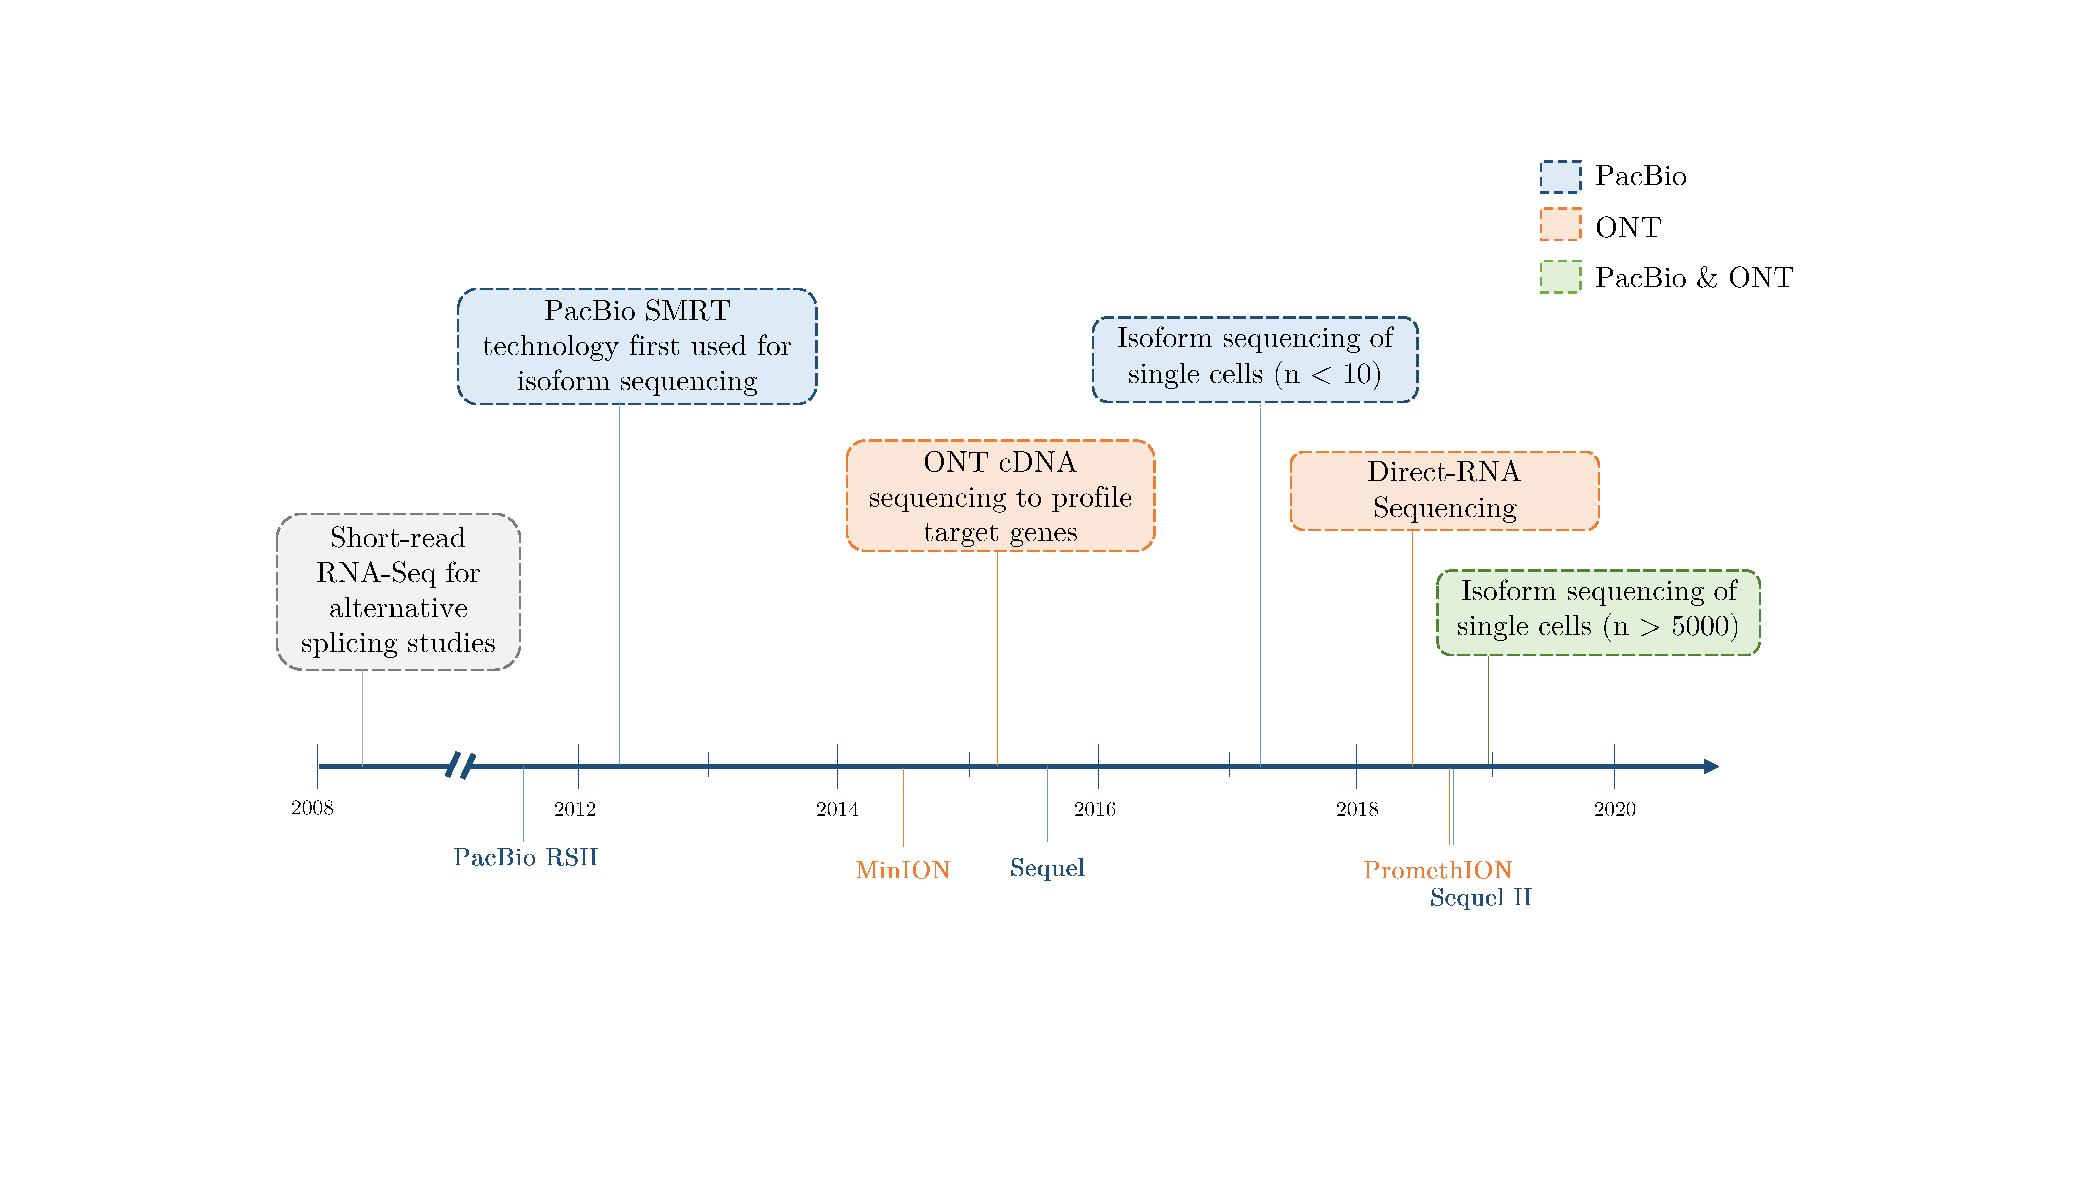
\includegraphics[page=1,trim={0 4cm 1.8cm 2cm},clip, scale = 0.8]{Figures/Introduction_Figures_Landscape.pdf}
			\captionsetup{margin={2cm,0cm}}
			\caption[Timeline of long read sequencing technology \& approaches]%
			{\textbf{Significant advances in long read sequencing technology \& approaches}: Major breakthroughs in long-read sequencing approaches of isoforms using Pacific Bioscience's (PacBio) Single molecule real-time sequencing (SMRT) (boxed blue) and Oxford Nanopore sequencing (ONT, boxed orange) are highlighted. Release of respective technologies are also marked }
			\label{fig:longread_timeline}
		\end{figure}
	\end{landscape}
	
	
	%\captionsetup{width=30cm}
	\begin{landscape}
		\small %smaller font
		\setlength\tabcolsep{2pt} %reduced margin size in table
		\renewcommand{\arraystretch}{1}
		\begin{longtable}[c]{p{4cm}p{4cm}p{18cm}}
			\caption[Long-read sequencing studies of single cells or direct RNA]%		
			{\textbf{Long-read sequencing studies of single cells or direct RNA}, DIE - differential isoform expression}
			\label{tab: longread_advancedstudies}\\
			
			\toprule
			\multicolumn{1}{c}{References} &
			\multicolumn{1}{c}{Samples and Tissue} &
			\multicolumn{1}{c}{Key Findings} \\* \midrule
			\endfirsthead
			%
			\endhead
			%
			\bottomrule
			\endfoot
			%
			\endlastfoot
			%								
			\centering Karlsson \& Linnarsson (2017)\cite{Karlsson2017} &
			\centering Mouse single cels (n = 6)  &
			\tabitem High isoform diveristy observed within single-cell oligodendrocytes with \textasciitilde1000 distinct isoforms mapped to 700 genes with low overlap between cells, predominantly driven by alternative TSS and TTS \\
			\hdashline[0.5pt/5pt]	
			
			\centering Gupta et al.(2018) \cite{Gupta2018} &
			\centering Mouse cerebellum (n = 1)  &
			\tabitem Long-read sequencing of >5000 single cells (microglia, astrocytes, neurons) after isolation \& barcoding \newline 
			\tabitem Identified cell-specific \textit{Bin1} isoforms with skipping of A1 and A2-A6 alternative exons (separated by constitutive exons) in all microglia, some astrocytes but not in neuronal cell-types, indicating cell-specific ES coordination \\
			\hdashline[0.5pt/5pt]			
			
			\centering Byrne et al. (2017)\cite{Byrne2017} &
			\centering Mouse single B1a cells (n = 7) &
			\tabitem Identified thousands of novel TSS and TTS (within 20bp bins due to lower error rate) \& hundreds of splicing events \newline
			\tabitem 160 genes with complex isoforms, 55 of which showed differential isoform usage (including B cell receptors) \\
			\hdashline[0.5pt/5pt]
			
			\centering Volden et al. (2018) \cite{Volden2018} &
			\centering Human single B cells (n = 96 from 1 donor) &
			\tabitem Circularising input cDNA and generating a CCS read (R2C2) significantly improved raw (316,000 cDNA reads at 94\% accuracy) and splice site accuracy (92\% vs ONT 1D raw reads at 80\%, Iso-Seq CCS reads at 97\%, based on SIRVs) \newline 
			\tabitem Ability to accurately demultiplex reads based on 7-8nt barcodes enabling mass sequencing of single cells with accurate gene quantification (strongly correlated with RNA-Seq, r = 0.79) and identification of cell-specific isoforms \\
			\hdashline[0.5pt/5pt]
			
			
			\centering Garalde et al. (2018) \cite{Garalde2018} &
			\centering Yeast \newline ERCC RNA-Spike in mix &
			\tabitem Direct RNA Sequencing of yeast poly(A) RNA achieved good coverage (2.8M reads vs 5.7M reads using ONT cDNA) with negligible effect on transcript length and GC content \newline 
			\tabitem Accurately identification of splice variants with no missing or novel exons from spike-in, and able to rudimentally discriminate RNA modification (m\textsuperscript{6}A, 5-mC) using trained datasets  \\
			
			\centering Workman et al. (2019) \cite{Workman2019a} &
			\centering Human B lymphocyte cell line (n = 30) &
			\tabitem Direct RNA-Sequencing of human cell line documented a high proportion (52.6\%) of novel isoforms \newline
			\tabitem High error rate (14\%) \& significant 5'truncation due to technical issues (rapid translocation through pore, signal artefacts from enzyme stalling or strand breaks), making it difficult to ascertain TSS \newline
			\tabitem Differences in poly(A) length distribution between mitochondrial and nuclear genes, and between different isoforms of the same gene (increase in polyA tail-lengths of intron-retaining isoforms) \\
			\hdashline[0.5pt/5pt]
			
			\centering Sessegolo et al. (2019) \cite{Sessegolo2019} &
			\centering Mouse brain \& liver \newline(n = 3) &
			\tabitem Benchmark study of Illumina RNA-Seq, ONT cDNA-Seq with/without 5'cap, \& ONT Direct RNA-Seq. \newline
			\tabitem Biased ONT cDNA-Seq of truncated transcripts with internal runs of poly(T) (15nt) due to cDNA synthesis; ONT RNA-Seq most accurately quantified gene expression using spike-in, followed by RNA-Seq, cDNA-Seq  \\
			\hdashline[0.5pt/5pt]
			
			\centering Singh et al. (2019) \cite{Singh2019} &
			\centering Human T- \& B-cell lines \newline Tumour \& paired lymph node (n = 1)  &
			\tabitem Novel sequencing method (RAGE-Seq) combining droplet-based scRNA-Seq with target capture ONT cDNA-Seq \newline 
			\tabitem Able to differentiate naive and mature B cells, and subpopulation by accurate identification of antigen receptor; track clonally related cells across tissues revealing cell-specific expression changes between tumour \& lymph node \\
			\hdashline[0.5pt/5pt]
			
			\centering Joglekar et al. 2021 \cite{Joglekar2021} &
			\centering Mouse hippocampus \& prefrontal cortex (n = 2) &
			\tabitem Identified $\tilde{400}$ DIE genes between brain regions using gene-wise test (nx2 table with isoform counts per gene), which was governed predominantly by splice variant changes in one single cell type \newline 
			\tabitem Spatial transcriptomics with Iso-Seq (Sl-ISO-Seq) confirmed localisation of brain-region specific DIE (exon-based). 
			\\* \bottomrule
		\end{longtable}
	\end{landscape}
\end{changemargin}



\newpage
\section{Aims and Objectives}
An increasing number of studies implicate a role of alternative splicing in AD disease development and pathogenesis (reviewed in \cref{tab: AS_ADHuman_studies}). However, such transcriptional profiling studies are typically performed using standard short-read RNA-Sequencing, which is inherently-constrained at transcript assembly and subsequent isoform characterisation essential for splicing analysis (described in \cref{rnaseq_intro}). My PhD thus aims to overcome these challenges by leveraging the use of long-read sequencing to accurately characterise isoform diversity and splicing patterns associated with Alzheimer's disease (\cref{fig:studydesign})

%Further limitations of RNA-Seq studies
%By identifying and characterising such alternative splicing events, there is hope of deepening current understanding of the biological role of transform isoform diversity and in the case of AD, identify novel pathways involved in pathogenesis of disease as potential target treatments. 

\textbf{Hypothesis}: Transcriptomic dysregulation plays a fundamental role in development of AD pathology. This includes alterations in gene splicing, which results in differential and novel expression of transcripts that are translated to generate isoforms with functional biological implications. 

\textbf{Main Objectives}:

\begin{enumerate}[]
	\item Optimise long-read sequencing approaches, PacBio's Iso-Seq and ONT cDNA sequencing, for profiling of full-length transcripts (\cref{ch: long_read_sequencing}) 
	\item Characterise isoform diversity and splicing events in mouse cortex globally using optimised long-read sequencing approaches (\cref{ch: whole_transcriptome}) 
	\item Identify global,age-related transcriptional and splicing changes associated with progression of tau pathology using well-characterised AD mouse model, rTg4510 (\cref{ch: transcriptional_global_differences})
	\item Comprehensively characterise isoform diversity and splicing events of 20 AD-associated genes, and changes in transcript expression associated with tau pathology in rTg4510 mice (\cref{ch: targeted_transcriptome})
	\item Identify AD-associated differential splicing and transcript expression in human post-mortem brain tissue and relate findings to those identified in mouse (\cref{ch: BDR})
	\item Integrate transcriptomic analyses with epigenetic (\cref{ch: targeted_transcriptome}) and proteomic data (\cref{ch: BDR}), available from the same samples
\end{enumerate}
% Integrative Papers
% https://www.nature.com/articles/s41588-020-00773-z importance of linking genomics with proteomics
% https://www.nature.com/articles/s41591-020-0815-6 - more proteomics
% https://www.nature.com/articles/s41588-020-0696-0 - epigenetics


\begin{landscape}
	\begin{figure}[htb]
		\begin{center}
			\includegraphics[page=2,trim={0 0 0 0},clip,scale = 0.7]{Figures/Introduction_Figures_Landscape.pdf}
		\end{center}
		\captionsetup{width=1.5\textwidth}
		\caption[Study design and analysis overview]%
		{\textbf{Study design and analysis overview}. To identify transcriptional and splicing changes associated with AD pathology, this thesis aims to characterise isoform diversity and splicing events at a global and targeted level from the rTg4510 mouse model and AD human post-mortem brain tissues. ONT - Oxford Nanopore Technology, PacBio Iso-Seq - Pacific Bioscience's Isoform Sequencing}
		\label{fig:studydesign}
	\end{figure} 	
\end{landscape}
\chapter{General Methodology}\label{ch: general methodology}

This chapter describes the general methods that were applied in the long-read sequencing experiments in \textbf{Chapters 4,6 and 7}. Experimental methods specific to individual results chapters can be found in the Methods section of the relevant chapter. Methods pertaining to the library preparation for PacBio Isoform Sequencing (Iso-Seq) and ONT Nanopore cDNA sequencing can be found in \cref{chap:isoseq_labpipeline} and \cref{chap:ont_labpipeline}, respectively. Standard manufacturer's protocols used in my thesis can be found in \textbf{Appendix \ref{app_longread_protocol} and \ref{app_longread_ont_protocol}}. All reagents mentioned in this Chapter were provided with the respective kits unless otherwise stated.

\section{Mouse tissue samples and \& RNA Isolation}

\subsection{Mouse model of AD tauopathy: rTg4510} 
\label{ch2: rtg4510}
rTg4510 mice recapitulate AD tauopathy through the overexpression of the human tau transgene, MAPT\textsuperscript{P301L}, which harbours the FTD-associated P301L mutation. It contains four microtubule-binding domains while lacking the N-terminal segment (4R0N), and exons 2-3 of the mouse prion protein gene \textit{Prnp}. The transgene expression is controlled under the calcium calmodulin kinase II promoter (CaMK2a) and is largely restricted to the forebrain, with age-dependent spread of neuropathology starting from as early as 2 months in the neocortex to rapid progression in the hippocampus by 5 months (\cref{fig:immunohistochemistry}). Neuronal and synaptic loss is also observed by 9 months, with these mice exhibiting cognitive and behavioural impairments. Sex differences in pathology have been reported with female mice exhibiting earlier and more severe cognitive and behavioural impairments than transgenic male mice\cite{M2011}. 

The rTg4510 mouse model is particularly informative as tau expression can be induced through the tetracycline operon-responsive element and suppressed upon doxycycline treatment\cite{Ramsden2005}. However, a recent study reported disruption of several endogenous mouse genes due to the random integration of MAPT\textsuperscript{P301L}, which has additional off-target effects that may potentially contribute to the neurodegenerative phenotype associated with rTg4510 transgenic mice\cite{Gamache2019}. 
 

\subsection{Animal breeding \& Sample Preparation}
\label{sec: animalbreeding_sample preparation}
All animal procedures were carried out at Eli Lilly and Company (Windlesham, UK), in accordance with the UK Animals (Scientific Procedures) Act 1986 and with approval of the local Animal Welfare and Ethical Review Board. The mice were housed under standard conditions (constant temperature and humidity with a 12h light/dark cycle in individually ventilated cages) before terminal anaesthesia with pentobarbital and transcardial perfusion with phosphate-buffered saline (PBS)\cite{Castanho2020}

The entorhinal cortex was dissected from the left-brain hemisphere of female transgenic mice (TG\nomenclature{TG}{Transgenic mice}) and wild-type controls (WT\nomenclature{WT}{Wild-type mice}), aged 2, 4, 6 and 8 months (n = 9-10 mice per group). Total RNA was then extracted\cite{Castanho2020} using the AllPrep DNA/RNA Mini Kit (Qiagen) according to the manufacturer's protocol, and converted to cDNA for library preparation (described later in \cref{section:ch2_cDNA_synthesis_explanation}). Of note, more than 80\% of total RNA is comprised of ribosomal RNA (rRNA), with the remaining 15\% representing transfer RNA (tRNA) and only 1-5\% representing mRNA. 

\begin{landscape}
	\begin{figure}[htp]
		\centering
		\vspace{20pt}
		\includegraphics[page=3,trim={0 7cm 0 0 },clip, scale = 0.7]{Figures/Introduction_Figures_Landscape.pdf}
		\captionsetup{width=1.5\textwidth}
		\caption[Progressive increase in tau in the hippocampus and entorhinal cortex of rTg4510 TG mice]%
		{\textbf{Progressive increase in tau in the hippocampus and entorhinal cortex of rTg4510 TG mice.} \textbf{A)} Representative immunohistochemistry images from the hippocampus showing accumulation of tau pathology in rTg4510 transgenic (TG) mice compared with wild-type (WT) control mice at 2, 4, 6, and 8 months of age. \textbf{B)} Progressive increase in tau is observed the hippocampus and the \textbf{C)} entorhinal cortex in rTg4510 TG but not WT animals. Figures and legends are adapted from Castanho et al. 2020 \cite{Castanho2020}}
		\label{fig:immunohistochemistry}
	\end{figure}	
\end{landscape}

\subsection{Assessment of nucleic acid quality and quantity}
Acquiring high-quality RNA, generating full-length cDNA and successfully performing the multi-step library preparation are all crucial for optimal sequencing experiments, particularly long-read sequencing. The assessment of the purity and integrity of extracted RNA, followed by cDNA quality and quantity, was therefore required throughout the library preparation and quality control (QC) stages of my sequencing experiments. This was undertaken using the RNA/DNA ScreenTape and Bioanalyzer assays for qualitative assessment, and the Qubit for DNA quantification. 


\subsection{ScreenTape \& Bioanalyzer assays}
\label{section:ch2_bioanalyzer} 
ScreenTape and Bioanalyzer assays are commonly used to provide an accurate and automated assessment of nucleic acid quality and size by electrophoresis. It works on the principle that upon applying an electric field, negatively-charged DNA migrates through a gel matrix towards the positive anode at a rate that is dependent on DNA size; smaller DNA fragments migrate faster, and thus move further through the gel within a specific time frame. The separated DNA can be then visualised using a fluorescent dye that intercalates into the double-stranded DNA (dsDNA\nomenclature{dsDNA}{double-stranded DNA}) structure and fluoresces under ultraviolet light. 

Both RNA ScreenTape and Bioanalyzer assays further provide a numeric evaluation of the quality of an RNA sample using a score between 1 and 10 , known as a RNA Integrity Number (RIN\nomenclature{RIN}{RNA Integrity Number}); a RIN score of 1 is indicative of high degradation and poor quality RNA, whereas a RIN score of 10 indicates minimal degradation (\cref{fig:bionalayzer_pics}). The purity and quantity of extracted RNA was assessed using the RNA Bioanalyzer assay with Agilent RNA 6000 Nano Kit (Agilent Technologies) and Agilent 2100 Bioanalyzer instrument (Agilent Technologies). 

Assessment of cDNA quality during various QC stages of long-read library preparation was mostly performed using the DNA Bioanalyzer assay with Agilent D1200 Kit (Agilent Technologies), particularly where accurate determination of library molarity was critical given the Bioanalyzer assay is more sensitive than the ScreenTape assay. However in QC stages where assessment is optional, the D5000 ScreenTape (Agilent Technology) and 4200 TapeStation (Agilent Technology) were used instead as the ScreenTape assay is most cost-effective and quicker to run. Both assays were performed following the standard manufacturer's protocol. Briefly, this involved mixing the sample with the ladder and buffer (if using the ScreenTape), or with the marker and gel-dye mix (if using the Bioanalyzer assay), before loading the sample into the machine to be assayed. Detailed lab instructions for Bioanalyzer and ScreenTape assays are detailed in \textbf{Appendix \ref{Isoseq_Protocol_tapestation_bioanalyzer}}.

\subsection{Qubit}
\label{section:ch2_qubit}   
Qubit assays (Invitrogen) allow accurate nucleic acid quantification by the selective binding of fluorescent Qubit dyes to dsDNA or RNA, rendering it more sensitive and specific than the NanoDrop 8000 spectrophotometer (Thermo Fisher Scientific) which uses UV absorbance. Following RNA extraction, the RNA concentration was determined using Qubit assays to ensure that the same amount of total RNA for each sample was used for library preparation. Many of the QC steps post DNA purification (later discussed in \cref{section:ch2_AMPure_explanation}) throughout library preparation also required Qubit assays to determine the cDNA concentration prior to proceeding with downstream experiments. Briefly, this involved running two "standard samples" prepared with Qubit reagent in 10:200 ratio, and the "test samples" prepared with the same reagent in a 1:200 ratio, on the Qubit 3.0 Fluorometer (Thermo Fisher Scientific) following the standard manufacturer's protocol (detailed in \textbf{Appendix  \ref{Isoseq_Protocol_qubit}}). Of note, all the quantity assessment in this thesis were performed with the Qubit DNA High sensitivity assay.          

\begin{figure}[htp]
	\centering
	\vspace{20pt}
	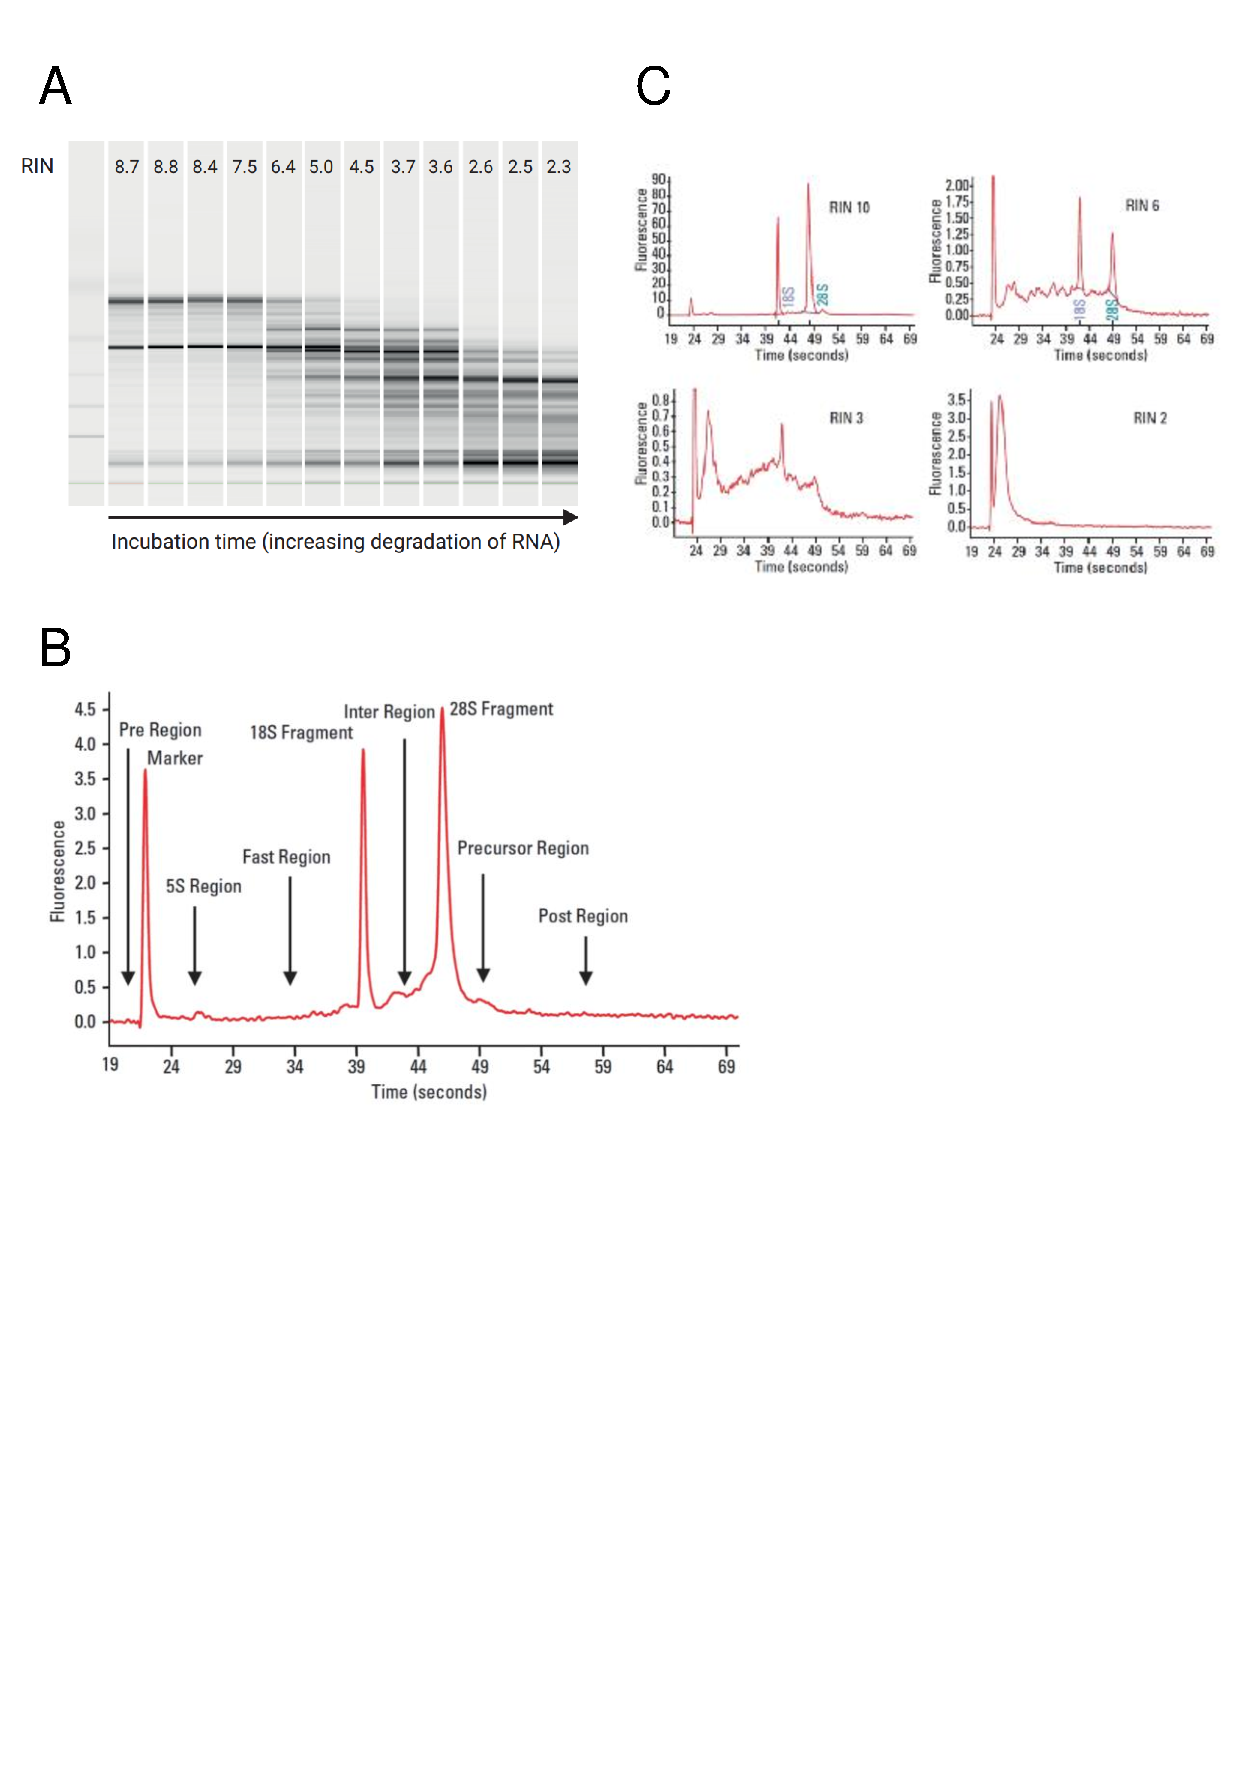
\includegraphics[page=1,trim={0 10cm 0 0 },clip, scale = 0.7]{Figures/General_Methodology_Figures.pdf}
	\captionsetup{width=0.95\textwidth}
	\caption[Evaluation of RNA integrity with ScreenTape \& Bioanalyzer assays]%
	{\textbf{Evaluation of RNA integrity with ScreenTape \& Bioanalyzer assays.} \textbf{A)} Shown is a gel image from a Bioanalyzer assay demonstrating progressive total RNA degradation over prolonged incubation time, which is indicated by a general shift to the right with more bands representing shorter fragments and a decrease in RIN number. \textbf{B)} An alternative assessment of total RNA quality and integrity is represented with the Bioanalyzer electropherogram with 2 distinctive peaks corresponding to 18S and 28S fragment of rRNA, and a marker peak. The RIN number is calculated by the relative ratio of the Fast Region and 18S, 28S fragment. \textbf{C)} Bioanalyzer electropherograms depicting total RNA with varying degrees of degradation: i) minimal (RIN = 10) as indicated by the two distinct peaks corresponding to 18S and 28S, ii) small degree (RIN = 6) with the two peaks still visible but there is presence of other smaller peaks, corresponding to fragmented RNA, iii) large degree of degradation (RIN = 3) with inability to detect the two peaks, and iv) maximum degradation (RIN = 2), indicated by the lack of large fragments. Figures and legends are adapted from Mueller et al. (2016)}
	\label{fig:bionalayzer_pics}
\end{figure}

\newpage
\section{cDNA synthesis, amplification \& purification}
After RNA isolation, integrity assessment and quantification, total RNA was converted to cDNA. Given the low frequency of mRNA (<5\% of total RNA) and low sensitivity of current sequencing platforms, the converted cDNA was subsequently amplified using Polymerase Chain Reaction (PCR\nomenclature{PCR}{Polymerase Chain Reaction}) and assessed using agarose gel electrophoresis. 


\subsection{Complementary DNA synthesis}
\label{section:ch2_cDNA_synthesis_explanation} 
Recommended as part of the Iso-Seq protocol, the SMARTer PCR cDNA Synthesis Kit (Clontech) was used to convert 200ng total RNA to cDNA. Unlike other cDNA synthesis methods,the SMARTer PCR cDNA synthesis relies on a modified oligo(dT) primer and a reverse transcriptase (RT\nomenclature{RT}{Reverse Transcriptase}) that has an inherent terminal transferase activity (outlined in \cref{fig:cDNAsynthesis_workflow}). First-strand synthesis therefore occurs in a SMART (\underline{S}witching \underline{M}echanism \underline{A}t 5' End of \underline{R}NA \underline{T}ranscript) fashion, whereby a few additional nucleotides ("overhang") are added to the 3' end of the cDNA as the RT approaches the 5' end of the mRNA. The RT then switched templates and continues replicating to the end, generating a full-length single-stranded cDNA which is then amplified. The usage of the "overhang" sequence ensured synthesis and enrichment of full-length cDNA, as cDNA without this sequence (i.e. prematurely terminated cDNA, cDNA from non poly(A) RNA, contaminating genomic DNA) will not be exponentially amplified \cite{Ramskold2012}. Detailed manufacturer's instructions of this kit can be found in \textbf{Appendix \ref{Isoseq_protocol_cDNAsynthesis}}. 

While this kit is advantageous in preferentially enriching for full-length cDNA sequences, it cannot differentiate between intact and truncated RNA; this would be present in poor-quality samples and amplified as technical artefact in the final cDNA library. One alternative is to exploit the 5’-cap that is present only in intact RNA (5'-cap refers to 7-methylguanosine at the 5’ end of mRNA which is added during transcription to protect nascent mRNA from degradation and assist in protein translation), using the Full-Length cDNA Amplification kit (Teloprime)\cite{Cartolano2016}. This kit relies on a double-stranded adapter that recognises and ligates to the 5’cap at the end of first-strand synthesis. I trialled this kit as part of my experiments, but was unable to generate cDNA. 

\begin{figure}[htp]
	\centering
	\vspace{20pt}
	\includegraphics[page=2,trim={0 12cm 0 0 },clip, scale = 0.7]{Figures/General_Methodology_Figures.pdf}
	\captionsetup{width=0.95\textwidth,singlelinecheck=off}
	\caption[Flowchart of SMARTer cDNA synthesis]%
	{\textbf{Flowchart of SMARTer cDNA synthesis.} SMARTer cDNA synthesis ensures the generation of full-length cDNA by the usage of the enzyme terminal transferase activity; premature termination of RT results in less efficient transferase activity and subsequent absence of overhang for downstream amplification. 
	cDNA synthesis is achieved in the following manner: 
	\begin{enumerate}
		\item Oligo(dT) primer (3’ SMART CDS Primer II A) primes the first-strand synthesis reaction by binding to polyA tail and transcribes the RNA into single-stranded DNA
		\item As RT reaches the 5’ end of the mRNA, the enzyme’s terminal transferase activity adds a few additional nucleotides to the 3’ end of the cDNA
		\item With a 3’end that is complementary to the added nucleotides, the SMARTer Oligonucleotide, or the template switching oligo, base-pairs with it and creates an extended template
		\item RT then switches templates and continues transcribing to the end of the SMARTer oligonucleotide 
		\item The resulting full-length, single-stranded cDNA contains the complete 5’ end of the mRNA, as well as a 3’ end that is complementary to the SMARTer Oligonucleotide. 
		\item The SMARTer Oligonucleotide and the poly A sequence then serves as universal priming sites for end-to-end cDNA amplification.
		\\
		
	\end{enumerate}
	Of note, the SMARTer II A Oligonucleotide, 3’ SMART CDS Primer II A, and 5’ PCR Primer II A all contain a stretch of identical sequence.  

	Figure and legend are taken from the SMARTer PCR cDNA Synthesis Kit User Manual\cite{LaboratoriesInc}. RT - Reverse Transcriptase.
	}
	\label{fig:cDNAsynthesis_workflow}
\end{figure}


\begin{landscape}
	To maximise throughput and minimise cost, my targeted experiments (\textbf{Chapters 6 and 7}) involved sequencing multiple samples simultaneously in one sequencing run (i.e. in “multiplex”). To differentiate the samples, I used a unique barcoded oligo(dT) primer for each sample for cDNA synthesis rather instead of the standard oligo (dT) primer from the SMARTer cDNA synthesis kit (Clontech) (\cref{tab:barcode_primers}). The only difference between the barcoded oligo(dT) and the standard oligo(dT) primer is the addition of a unique 16-bp internal barcode, which does not interfere with priming and end-to-end cDNA amplification. The general structure of the barcoded oligo(dT) primer is as follows:
	
	\hspace{5cm} \textcolor{RedOrange}{Primer Sequence} \hspace{2cm}   \textcolor{ForestGreen}{16-bp barcode}   \hspace{2cm} \textcolor{RoyalBlue}{oligo-dT}
	\vspace{-0.5cm}
	\begin{center}
		5'\textcolor{RedOrange}{AAGCAGTGGTATCAACGCAGAGTAC}\textcolor{ForestGreen}{tcagacgatgcgtcat}\textcolor{RoyalBlue}{TTTTTTTTTTTTTTTTTTTTTTTTTTTTTTVN3’}
	\end{center}

	\vspace{1cm}
	\begin{table}[ht]
		\centering
		\captionsetup{justification=raggedright,width=1.5\textwidth}
		\caption[Barcoded oligo(dT) primers for targeted transcriptome sequencing]%
		{\textbf{Barcoded oligo(dT) primers were used for multiplexing samples in targeted transcriptome sequencing}. Each of the barcoded primers contain the same 5' primer sequence and oligo-dT for reverse transcription of first strand cDNA synthesis using SMARTer PCR cDNA Synthesis Kit (Clontech). The barcodes were provided from the official PacBio multiplex protocol.}
		\label{tab:barcode_primers}
		\begin{tabularx}{1.5\textwidth}{cc}
			\toprule
			Barcode Name & Sequence                                                                  \\ \midrule
			Barcode 1    & AAGCAGTGGTATCAACGCAGAGTACCACATATCAGAGTGCGTTTTTTTTTTTTTTTTTTTTTTTTTTTTTTVN \\
			Barcode 2    & AAGCAGTGGTATCAACGCAGAGTACACACACAGACTGTGAGTTTTTTTTTTTTTTTTTTTTTTTTTTTTTTVN \\
			Barcode 3    & AAGCAGTGGTATCAACGCAGAGTACACACATCTCGTGAGAGTTTTTTTTTTTTTTTTTTTTTTTTTTTTTTVN \\
			Barcode 4    & AAGCAGTGGTATCAACGCAGAGTACCACGCACACACGCGCGTTTTTTTTTTTTTTTTTTTTTTTTTTTTTTVN \\
			Barcode 5    & AAGCAGTGGTATCAACGCAGAGTACCACTCGACTCTCGCGTTTTTTTTTTTTTTTTTTTTTTTTTTTTTTTVN \\
			Barcode 6    & AAGCAGTGGTATCAACGCAGAGTACCATATATATCAGCTGTTTTTTTTTTTTTTTTTTTTTTTTTTTTTTTVN \\
			Barcode 7    & AAGCAGTGGTATCAACGCAGAGTACTCTGTATCTCTATGTGTTTTTTTTTTTTTTTTTTTTTTTTTTTTTTVN \\
			Barcode 8    & AAGCAGTGGTATCAACGCAGAGTACACAGTCGAGCGCTGCGTTTTTTTTTTTTTTTTTTTTTTTTTTTTTTVN \\
			Barcode 9    & AAGCAGTGGTATCAACGCAGAGTACACACACGCGAGACAGATTTTTTTTTTTTTTTTTTTTTTTTTTTTTTVN \\
			Barcode 10 & AAGCAGTGGTATCAACGCAGAGTACACGCGCTATCTCAGAGTTTTTTTTTTTTTTTTTTTTTTTTTTTTTTVN \\ \bottomrule
		\end{tabularx}
	\end{table}
\end{landscape}


\subsection{Polymerase Chain Reaction (PCR)}
\label{section:ch2_PCR_explanation} 
The PCR is a well-established method for generating multiple copies of the same DNA sequence. Mimicking natural DNA replication, this relies on a thermostable DNA polymerase, a set of primers specific to the region of interest, and a cocktail of reagents required for polymerisation (i.e. deoxynucleotides (dNTPs)\nomenclature{dNTPs}{Deoxynucleotides} and buffers). This reaction is subjected to a series of heating and cooling steps: 
\begin{enumerate}
	\item Denaturation at 96$^{\circ}$C to separate dsDNA 
	\item Annealing, typically between 55$^{\circ}$C  and 65$^{\circ}$C, for the binding of primers to the complementary sequences on the single-stranded DNA; the specific annealing temperature is dependent on the primer sequence. 
	\item Extension at 72$^{\circ}$C to allow the polymerase to extend the primers, synthesising a new cDNA strand using dNTPs
\end{enumerate} 
These three steps are then repeated multiple times, or "cycles", resulting in an exponential generation of the DNA template of interest.

\subsection{Agarose Gel Electrophoresis}
\label{section:ch2_agarose_explanation}  
Agarose gel electrophoresis allows the separation of dsDNA molecules based on length, and works on the same principle as the Bioanalyzer and ScreenTape assays (described previously in \cref{section:ch2_bioanalyzer}). It is most commonly used to determine DNA quality and quantity, and assess the efficiency of molecular biology techniques such as PCR amplification in determining the number of optimum cycles. It is a well known phenomenon that an increased number of unnecessary PCR cycles can generate artefacts (strand invasion) and preferentially amplify shorter transcripts\cite{Acinas2005,Bayega2018}. Instructions to prepare and run an agarose gel electrophoresis are detailed in \textbf{Appendix \ref{Isoseq_Protocol_running_agarose_gel}}.


\subsection{AMPure Bead Purification} 
\label{section:ch2_AMPure_explanation} 
At various stages of long-read library preparation, cDNA was purified using AMPure beads (\cref{fig:ampure_bead_workflow}\textbf{A}). These are paramagnetic beads that reversibly bind to DNA in the presence of polyethylene glycol (PEG) and salt. The concentration of PEG, and consequent ratio of beads to DNA, determines the size of fragments that are bound and subsequently eluted (\cref{fig:ampure_bead_workflow}\textbf{B}); the lower the concentration of beads to DNA, the greater the proportion of longer DNA fragments bound, due to the preferential binding of beads to larger molecular weight DNA with a higher negative charge - a 0.4X ratio would therefore retain only the larger DNA fragments whereas a 1X ratio would retain both long and short DNA fragments (\cref{fig:ampure_bead_workflow}\textbf{B}). Briefly, AMPure Bead purification was performed by thoroughly mixing and vortexing each sample with a pre-specified ratio of AMPure beads. The samples were then placed onto a magnet for clear separation of DNA-bound beads and solution, followed by two washes of 70\% ethanol and DNA elution. Detailed instructions can be found in \cref{general_ampure_bead_purification}.

\begin{figure}[!h]
	\centering
	\includegraphics[page=3,trim={0 8cm 0 0cm},clip, scale = 0.7]{Figures/General_Methodology_Figures.pdf}
	\captionsetup{width=0.95\textwidth}
	\caption[DNA purification with AMPure beads]%
	{\textbf{DNA purification with AMPure beads}: A schematic figure depicting the \textbf{A)} steps of purifying DNA with AMPure Beads, with initial binding of magnetic beads to negatively-charged DNA enabling separation of DNA fragments, followed by ethanol wash and elution. \textbf{B)}) An agarose gel image of DNA purified using a range of bead to DNA ratio for size selection: lower ratio only retain longer fragments while shorter fragments are displaced. Figures are taken from Beckman Website.}
	\label{fig:ampure_bead_workflow}
\end{figure}

\clearpage
\section{ERCC-RNA Spike-In Controls}
\label{section:ch2_ERCC_explanation} 
A set of external RNA Spike-In controls, generated by the External RNA Controls Consortium (hereby referred to as "ERCC"\nomenclature{ERCC}{External RNA Controls Consortium}), was used to i) evaluate the performance of library preparation and the sequencing experiments, and ii) validate the Iso-Seq pipeline in accurately characterising the transcriptome using long reads. ERCC consists of 92 polyadenylated synthetic transcripts (250 to 2000 nucleotides) of known sequences from the ERCC plasmid library, which are added in pre-determined amounts to the sample prior to first-strand cDNA synthesis. The addition of ERCC allowed me to assess the quantitative power of long-read sequencing in addition to providing absolute quantification of mRNA isoforms (with the generation of a standard curve). It can further assess the validity of the bioinformatic analysis as only 1 isoform per ERCC should be detected. 

The amount of ERCC added was determined using the below equation \cite{WTAC}:
\begin{myequation}[!h]
	\begin{equation}
		\label{eqn:ercc_calcaluations}
		mass_{RNA spike} = fraction_{spiked reads}\; * fraction_{target RNA}\; *mass_{RNA input}
	\end{equation}
	\begin{equation}
		concentration_{RNA spike} = mass_{RNA spike}\; * volume_{RNA spike}
	\end{equation}
	where:
	\begin{conditions*}
		mass_{RNA spike} & mass of ERCC to be added to sample \\
		concentration_{RNA spike} & final diluted concentration (ng/$\mu$l) of ERCC \\
		fraction_{spiked reads}  &   desired proportion of sequenced ERCC reads relative to total amount of sequenced reads \textit{(3\%)} \\
		fraction_{target RNA}    &  expected proportion of target RNA, in this case mRNA relative to total RNA \textit{(3\%)} \\   
		mass_{RNA input} &  input of total RNA \textit{(200ng)} \\
		volume_{RNA spike} & volume of RNA spike-in \textit{(0.1$\mu$L)}				
	\end{conditions*}
	\captionsetup{width=0.95\textwidth}
	\caption[Determining the amount of ERCC-RNA Spike-In Control for sequencing runs]%
	{\textbf{Determining the amount of ERCC-RNA Spike-In Control for sequencing runs}. In determining the mass and final concentration of RNA-spike-in mix based on the above conditions, the stock ERCC RNA spike-in was diluted from the original concentration of 30ng/$\mu$L to 1.8ng/$\mu$L with a dilution factor of 1:16.8. The italicised parameters were taken from the RNA Transcriptomics 2018 Course\cite{WTAC} with the exception of total RNA input}
\end{myequation}

A separate pilot experiment (\textbf{Appendix \ref{ch:alt_cDNA}}) showed successful addition of ERCC with two main bands at \textasciitilde600bp and \textasciitilde1000bp (\cref{fig:ercc_lab_gel}a), reflecting significant enrichment of ERCC at these two respective lengths as expected (\cref{fig:ercc_lab_gel}b). However, the stark contrast of these two bands against the smear of cDNA suggests over-usage of ERCC - possibly due to the overestimation of assumed proportion of mRNA. A lower ERCC amount was therefore used across all the experiments to reduce unnecessary sequencing and coverage of ERCC (final concentration of 0.6ng/$\mu$L with a dilution factor of 1:50.5, \cref{fig:ercc_lab_gel}c). 

\vspace{1cm}
\begin{figure}[!htp]
	\begin{center}
		\includegraphics[page=4,trim={0 8cm 0 1cm},clip,scale = 0.65]{Figures/General_Methodology_Figures.pdf}
	\end{center}
	\captionsetup{width=0.95\textwidth}
	\caption[ERCC usage to benchmark library preparation and sequencing performance runs]%
	{\textbf{Successful addition of ERCC to first-strand cDNA synthesis. a)}An agarose gel image taken from PCR amplification of cDNA and ERCC (1.8ng/$\mu$L determined from equation \ref{eqn:ercc_calcaluations}), and ERCC alone as a positive control. 5$\mu$L of PCR aliquots were taken every cycle (13 - 18) and then run on gel electrophoresis. The two bands at 600bp and 1000bp correspond to the enrichment of ERCC at these two lengths as expected. \textbf{B)} Distribution of known ERCC length, with a significant proportion of transcripts sized at 500-600bp and 1000-1200bp. \textbf{C)} An agarose gel image after a repeat of PCR amplification of cDNA and ERCC at a lower concentration (0.6ng/$\mu$L) with ERCC as positive and water as negative control respectively. The numbers above the lanes refer to the number of PCR cycles. L denotes to 100bp Ladder.}
	\label{fig:ercc_lab_gel}
\end{figure}
 

\chapter{Long-read Sequencing}\label{ch: long_read_sequencing}

This chapter provides a detailed background into the lab workflow and bioinformatics pipeline used to generate and analyse data from Pacific Bioscience's (PacBio) SMRT Sequencing (henceforth referred to as Iso-Seq) and Oxford Nanopore Technology's nanopore cDNA sequencing. 

\section{Pacific Biosciences: Isoform Sequencing}
\label{sec:pb_isoform_sequencing}

\subsection{Introduction}
Successful DNA polymerisation requires a high concentration of nucleotides for DNA polymerase processivity and accuracy. However, mimicking this in DNA sequencing results in a high background noise level, thereby reducing the sensitivity to detect base incorporation and fluorophore emission. Historically, second-generation sequencing technologies such as Illumina RNA-Seq have circumvented this issue by the step-wise addition, scan and wash of each set of labelled nucleotides, though at the expense of read lengths (as discussed in \cref{rnaseq_intro}). 

In 2013, PacBio pioneered the development of third generation long-read sequencing with the capability to generate substantially longer reads (reviewed in \cref{tab: longread_isoseqstudies}), due to its ability to mimic the natural, uninterrupted, processive DNA synthesis through three important innovations\cite{Eid2009}: 
\begin{enumerate}
	\item The creation of a circular template, SMRTbell (\cref{fig:Mechanism}\textbf{A}), which is enclosed with hairpin adapters at the ends of the insert, allowing uninterrupted DNA polymerisation \cite{Travers2010}.
	\item Sequencing each polymerase-bound SMRTbell at the bottom of a nanometre-wide well (zero-mode-waveguide - ZMW\nomenclature{ZMW}{Zero-Mode-Waveguide})\cite{Levene2003} (\cref{fig:Mechanism}\textbf{B}). The nanoscale size of the ZMWs and reduced volume allow sensitive detection of a single nucleotide incorporation event against the high background of labelled nucleotides, achieving a high-signal-to-noise ratio. PacBio currently offers two sequencers, which primarily differs in the number of ZMWs that can be sequenced: Sequel I and Sequel II with 1M and 8M ZMWs, respectively.   
	\item The addition of phospholinked nucleotides, each labelled with a different colour fluorophore corresponding to the four different bases (A, C, G and T), which allows for natural and processive DNA synthesis\cite{Mccarthy2010} (\cref{fig:Mechanism}\textbf{C}). 
\end{enumerate}

\vspace{1cm}
\subsubsection{Mechanism}
Due to the circular nature of the SMRTbell template, the polymerase is able to continually read through the insert in an interrupted fashion multiple times (or "passes"), resulting in a continuous read (known as a polymerase read) (\cref{fig:Mechanism}\textbf{A}). By removing the hairpin-adapters that delineate the repeated insert sequence, this polymerase read is resolved to multiple reads (known as subreads), which are then merged to yield one high-quality and highly-accurate consensus read (known as a circular consensus sequence - CCS\nomenclature{CCS}{Circular Consensus Sequence}) (\cref{fig:Mechanism}\textbf{A}). The generation of these CCS reads can drastically improve a single-pass from 85\%, due to random sequencing error, to 99\% from alignment and correction of multiple subreads. Notably, the error rate is proportional to the number of "passes", and is dependent on the polymerase lifetime and insert length\cite{Travers2010}. 

Unlike RNA-Seq short reads, PacBio Iso-Seq reads are not of a set length, but a range of lengths that is reflective of the library size and polymerase activity\cite{Ardui2018,Rhoads2015}. Previous chemistries preferentially sequenced molecules of a certain length due to biased loading of SMRTbell templates; Diffusion Loading favoured shorter molecules\cite{Loomis2013} whereas Magbead Loading allowed proportional loading to the concentration rather than by length, but prevented sequencing of molecules <1kb (discussed in \cref{section:ch2_polbinding_loading}). However, recent improvements in both technology and chemistry have alleviated this sequencing read bias, eliminating the need for fractionating the library by length prior to sequencing (size selection) and resulting the Magbead loading method obsolete \cite{Oikonomopoulos2020}.

\begin{figure}[!h]
	\centering
	\includegraphics[page=14,trim={0 5cm 0 0 },clip, scale = 0.7]{Figures/ProjectDevelopment_Figures.pdf}
	\captionsetup{width=0.95\textwidth}
	\caption[Pacific Bioscience's Single Molecule Real-time Sequencing]%
	{\textbf{Pacific Bioscience's Single Molecule Real-time Sequencing (SMRT)}: PacBio's SMRT technology is able to generate long reads >10kb by \textbf{A)} enclosing the cDNA fragment of interest within a circular template (SMRTbell) to allow uninterrupted DNA polymerisation,  followed by the \textbf{B)} sequencing of each SMRTbell with a bound polymerase at the bottom of ZMWs, enabling sensitive detection of polymerisation at nucleotide level from \textbf{C)} addition of phospholinked nucleotides with differently labelled fluorophore. ZWW - Zero-Mode-Waveguide}
	\label{fig:Mechanism}
\end{figure}


\subsection{Lab Workflow}
\label{chap:isoseq_labpipeline}
This section describes the lab workflow for PacBio Iso-Seq library preparation, which was applied in the long-read sequencing experiments for global and targeted transcriptome profiling in \textbf{Chapters 4 and 6}, respectively. Methods pertaining to sample preparation, cDNA synthesis and amplification can be found in \cref{ch: general methodology}.

The Iso-Seq lab workflow for the global profiling of the transcriptome, as outlined in \cref{fig:isoseq_wholelab_protocol}, involved three main steps: i) converting RNA to full-length cDNA using the Clontech SMARTer PCR cDNA synthesis kit (\cref{section:ch2_cDNA_synthesis_explanation}), ii) amplification (\cref{section:ch2_PCR_explanation}) and purification (\cref{section:ch2_AMPure_explanation}) of double-stranded cDNA, and iii) performing SMRTbell library preparation. 

The Iso-Seq lab workflow for the targeted profiling of the transcriptome, outlined in \cref{fig:isoseq_targetedlab_protocol}, involved the usage of barcode sequences in cDNA synthesis to allow sample multiplexing and an additional step of target gene enrichment.

\vspace{3cm}
\begingroup
\parindent=0em
\etocsettocstyle{\rule{\linewidth}{\tocrulewidth}\vskip0.5\baselineskip}{\rule{\linewidth}{\tocrulewidth}}
\etocsetnexttocdepth{5}
\localtableofcontents 
\endgroup

\begin{figure}[htp]
	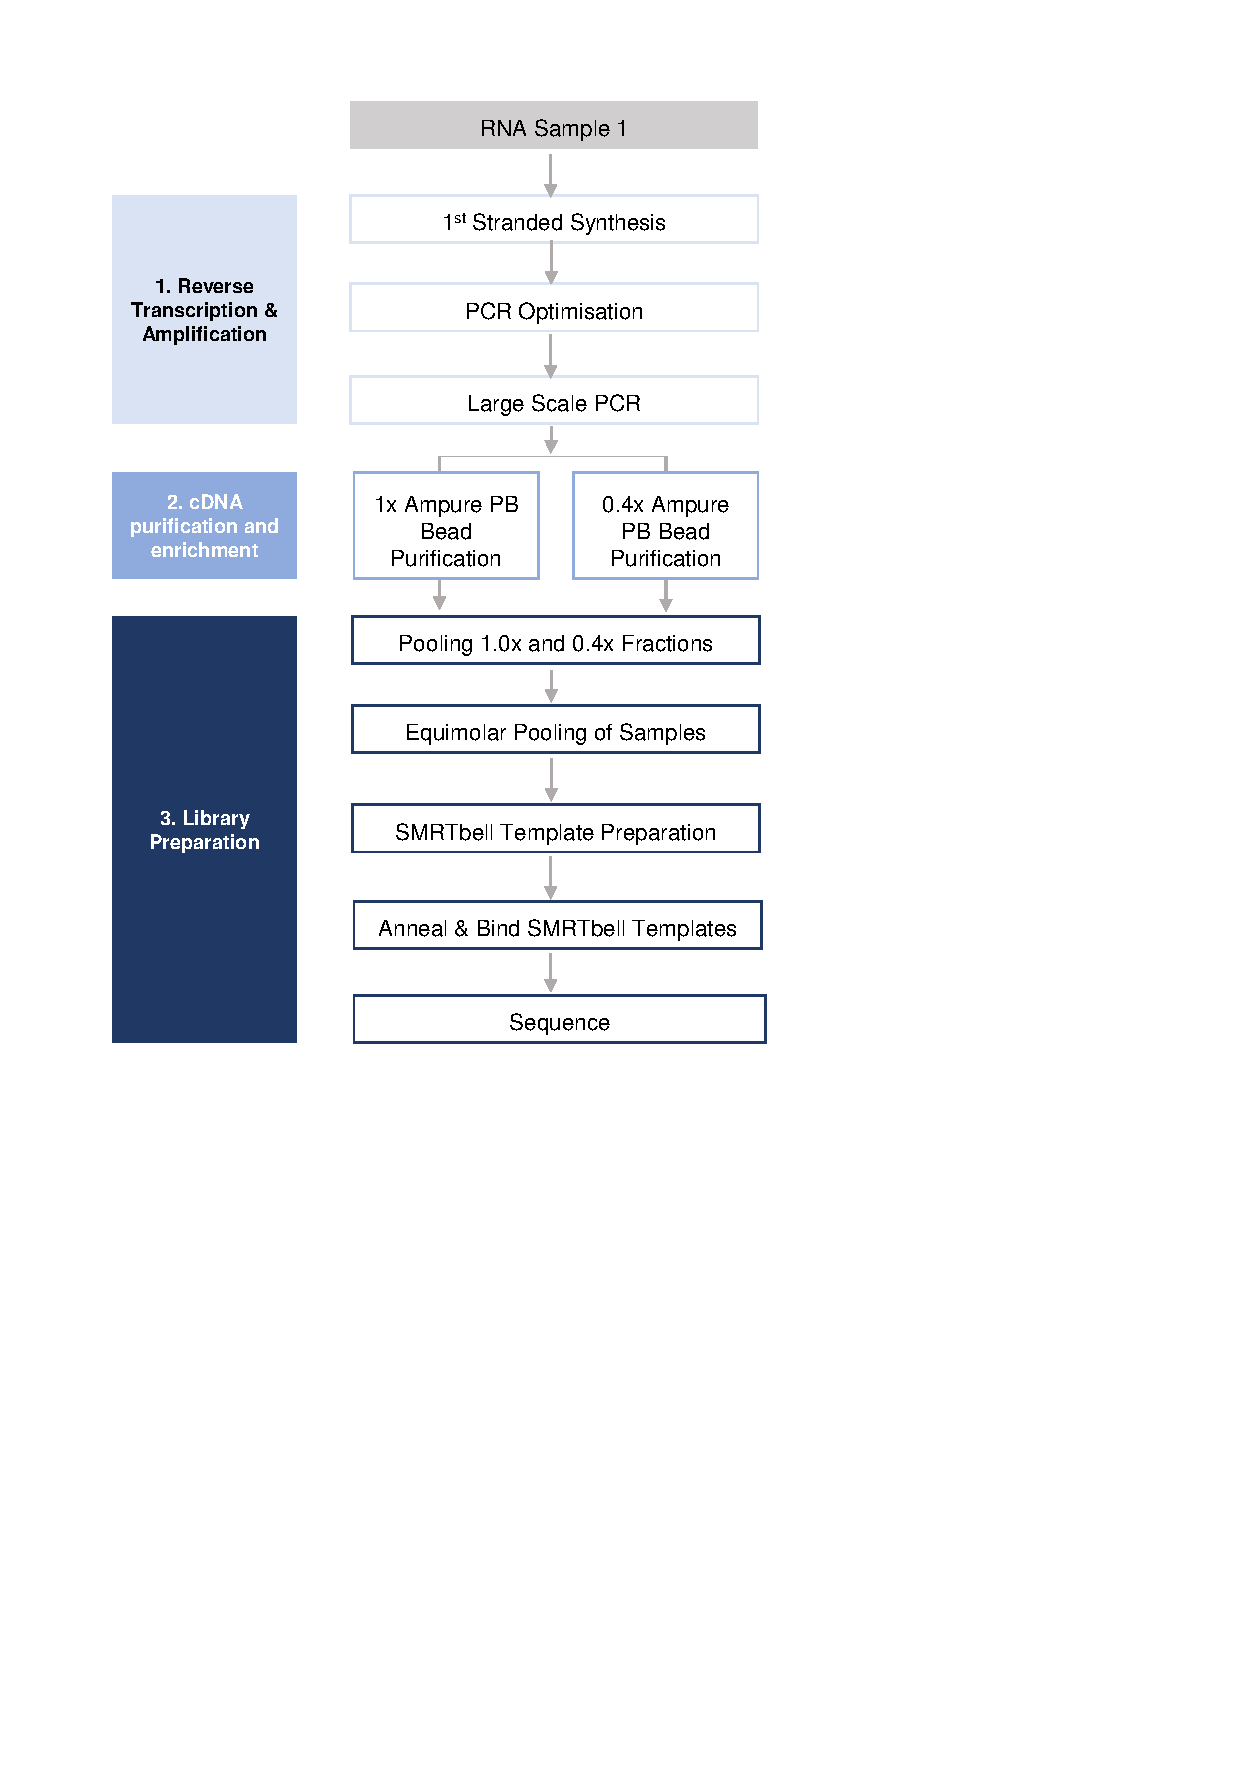
\includegraphics[page=1,trim={0 12cm 5cm 1cm},clip,scale = 1]{Figures/ProjectDevelopment_Figures.pdf}
	\captionsetup{width=0.95\textwidth}
	\caption[Iso-Seq Lab workflow for global transcriptome profiling]%
	{\textbf{An overview of the Iso-Seq lab workflow for global transcriptome profiling}. Shown is a flow diagram of the Iso-Seq lab workflow. Adapted from the official Iso-Seq protocol, it involves three main steps: 1) reverse transcription and amplification of cDNA (\cref{section:ch2_cDNA_synthesis_explanation}), 2) cDNA purification with AMPure beads (\cref{section:ch2_AMPure_explanation}) and 3) library preparation involving ligation of SMRTbell templates, and binding of the primer and polymerase (\cref{section:ch2_smrtbelltemplate_explanation}). Due to the usage of newer chemistries, size selection was not performed.}
	\label{fig:isoseq_wholelab_protocol}
\end{figure}

\begin{figure}[]
	\begin{center}
		\includegraphics[page=2,trim={1cm 11cm 1cm 1cm},clip,scale = 0.8]{Figures/ProjectDevelopment_Figures.pdf}
	\end{center}
	\captionsetup{width=0.95\textwidth}
	\caption[Iso-Seq Lab workflow used for targeted transcriptome profiling]%
	{\textbf{An overview of the Iso-Seq lab workflow for targeted transcriptome profiling}. Shown is a flow diagram of the Iso-Seq lab workflow for targeted transcriptome profiling, which follows a similar workflow as global transcriptome profiling (depicted in Figure \ref{fig:isoseq_wholelab_protocol}), with the addition of a target cDNA capture step (boxed orange, described in \cref{section:ch2_targetcapture_explanation}) and the use of barcode sequences in cDNA synthesis (boxed green and denoted here as Barcode 1 and Barcode n) to allow sample multiplexing. The list of barcodes can be found in \cref{tab:barcode_primers}}
	\label{fig:isoseq_targetedlab_protocol}
\end{figure}

\clearpage
\subsubsection{PCR optimisation and DNA Amplification}\label{ch: pcr_optimisation}
After cDNA synthesis, cDNA products were amplified using PCR to generate sufficient material for sequencing. To minimise PCR bias resulting in under or over representation of the different cDNA library size, the optimum number of PCR cycles for amplification was determined with PrimeSTAR GXL DNA Polymerase (Clontech) (\cref{fig:pcr_optimisation_gel_eg}). This involved collecting 5$\mu$L PCR aliquots every two cycles (cycles 10, 12, 14, 16, 18 and 20) followed by visualisation of cDNA products on a 1.5\% Agarose gel with ethidium bromide. The optimum cycle number was determined by the cycle that generated sufficient amount of cDNA without compromising on the molecular weight, which is typically observed with PCR over-amplification of cDNA (\cref{fig:pcr_optimisation_gel_eg}). Large scale PCR amplification was then subsequently performed using the optimum number of cycles. 

\begin{figure}[htp]
	\begin{center}
		\includegraphics[page=13,trim={1cm 24cm 10cm 1cm},clip,scale = 0.9]{Figures/ProjectDevelopment_Figures.pdf}
	\end{center}
	\captionsetup{width=0.95\textwidth}
	\caption[Example of an agarose gel for determining the optimum number of PCR cycles for amplification]%
	{\textbf{PCR optimisation is required to determine the optimum number of cycles}. Shown is an agarose gel of Human Brain Total RNA after first strand cDNA synthesis and PCR amplification through cycles 8 to 18, with PCR aliquots collected during every two cycles. In this example, 10 cycles were determined to be the optimum number for large-scale amplification. While smear distribution from 8 and 10 cycles look similar, 10 cycles show a slightly stronger smear, thereby generating more material for downstream pooling. Cycles above 12 show signs of over-amplification which will result in biased sequencing representation. Figure and legend are adapted from Iso-Seq protocol}
	\label{fig:pcr_optimisation_gel_eg}
\end{figure}


\subsubsection{AMPure Bead Purification} 
\label{section:ch2_ampurebead_pool} 
After large scale amplification, the resulting PCR products were divided into two fractions for purification with either 0.4X or 1X AMPure PB beads (PacBio). DNA purification with 0.4X AMPure beads was essential to ensure enrichment of longer fragments for sequencing (as described in \cref{section:ch2_AMPure_explanation}). Quantification and size distribution of each fraction was then determined using Qubit DNA High sensitivity assay (Invitrogen) (\cref{section:ch2_qubit}) and Bioanalyzer assays on the 2100 Bioanalyzer (Agilent) (\cref{section:ch2_bioanalyzer}) for calculating the molarity of the two fractions (using \textbf{Equation \ref{eqn:isoseq_library_molarity}}). Equal molar quantities of the two fractions were then pooled for library construction with the SMRTbell Template Prep Kit v1.0 (PacBio). 

\begin{equation}
	\label{eqn:isoseq_library_molarity}
	\frac{concentration(\frac{ng}{ul})\times 10^6}{660(\frac{g}{mol}) \times average\:library\:size\:in\:bp\mbox{*}} = concentration\;in\; nM
\end{equation}
* the average library size was determined by the start and end point of the cDNA smear on the BioAnalyzer

\subsubsection{Target Capture using IDT Probes} 
\label{section:ch2_targetcapture_explanation} 
Targeted profiling of the transcriptome was performed as part of the long-read sequencing experiments in \textbf{Chapter 6}. This first involved equimolar pooling of uniquely-barcoded samples, followed by enrichment of target genes with a hybridisation-based capture approach (IDT). Through this approach, regions of interest within the library were captured ("hybridised") with pre-designed, 5’ biotinylated, 120nt-long oligonucleotide baits (henceforth referred to as probes, \cref{fig:isoseq_targetcapture}\textbf{A}). Magnetic streptavidin beads were then used to isolate the hybridised library fragments for amplification (using Takara Hot-Start polymerase) and AMPure bead purification (outlined in \cref{fig:isoseq_targetcapture}\textbf{B}). After assessing the quality and quantity of the target cDNA with Qubit and Bioanalyzer assays, SMRTbell library preparation was proceeded according to manufacturer's protocol.  

%*Modifications to the protocol: waiting times at room temperature during hybridisation, lid heat temperatures, method of washing beads at room temperature; all modifications are incorporated from official IDT protocol, post amplification clean-up for consistency  

\myparagraph{Probe Designs}
Probes were designed to a selective panel of 20 AD-associated genes (henceforth referred to as target genes)): \textit{Abca7, Abca1, Ank1, Apoe, App, Bin1, Cd33, Clu, Fus, Fyn, Mapt, Picalm, Ptk2b, Rhbdf2, Snca, Sorl1, Tardbp, Trem2, Trpa1, Vgf}. Two separate pools of equimolar probes were designed against the mouse (GRCm28/mm10) and human genome (GRCh37/hg19). While IDT provided a pre-designed set of probes to the exons of target genes (depicted in \cref{fig:target_probes_eg}\textbf{A}), the majority of exons were unnecessarily covered by contiguous probes, which can induce off-target binding and additional costs. Given that previous targeted sequencing studies using the same hybridisation-based capture have achieved successful enrichment and sequencing with a few unique probes to the exonic region\cite{Sheynkman2020}, I manually assessed the list of probes for each target gene using the following criteria:
\begin{itemize}
	\item All of the exons must be covered by at least one probe
	\item Probes should be spaced 300-500bp within each exon (equivalent to 0.2x – 0.3x tiling density) 
	\item Probes with the highest GC content (40-65\% GC content) and lowest number of blast hits were selected from the contiguous cluster 
	\item Any probes covering the intronic regions were removed
\end{itemize}
Examples of the initial set of probes provided by IDT and the final curated sets are illustrated in  \cref{fig:target_probes_eg}\textbf{B - D}. 

\begin{figure}[!h]
	\begin{center}
		\includegraphics[page=12,trim={0cm 6cm 0cm 1cm},clip,scale = 0.70]{Figures/ProjectDevelopment_Figures.pdf}
	\end{center}
	\captionsetup{width=0.95\textwidth}
	\caption[Lab workflow for hybridisation-based cDNA capture for targeted transcriptome profiling]%
	{\textbf{Lab workflow for hybridisation-based cDNA capture for targeted transcriptome profiling.}. Shown is an overview of the lab workflow for target gene enrichment involving hybridisation of cDNA with probes and blockers (poly(T) oligonucleotide, cDNA synthesis primers), followed by isolation with streptavidin beads. The addition of blockers prevent non-specific binding, and subsequently increases capture rate and target gene sequencing coverage}
	\label{fig:isoseq_targetcapture}
\end{figure}

\begin{landscape}
	\begin{figure}[!ht]
		\begin{center}
			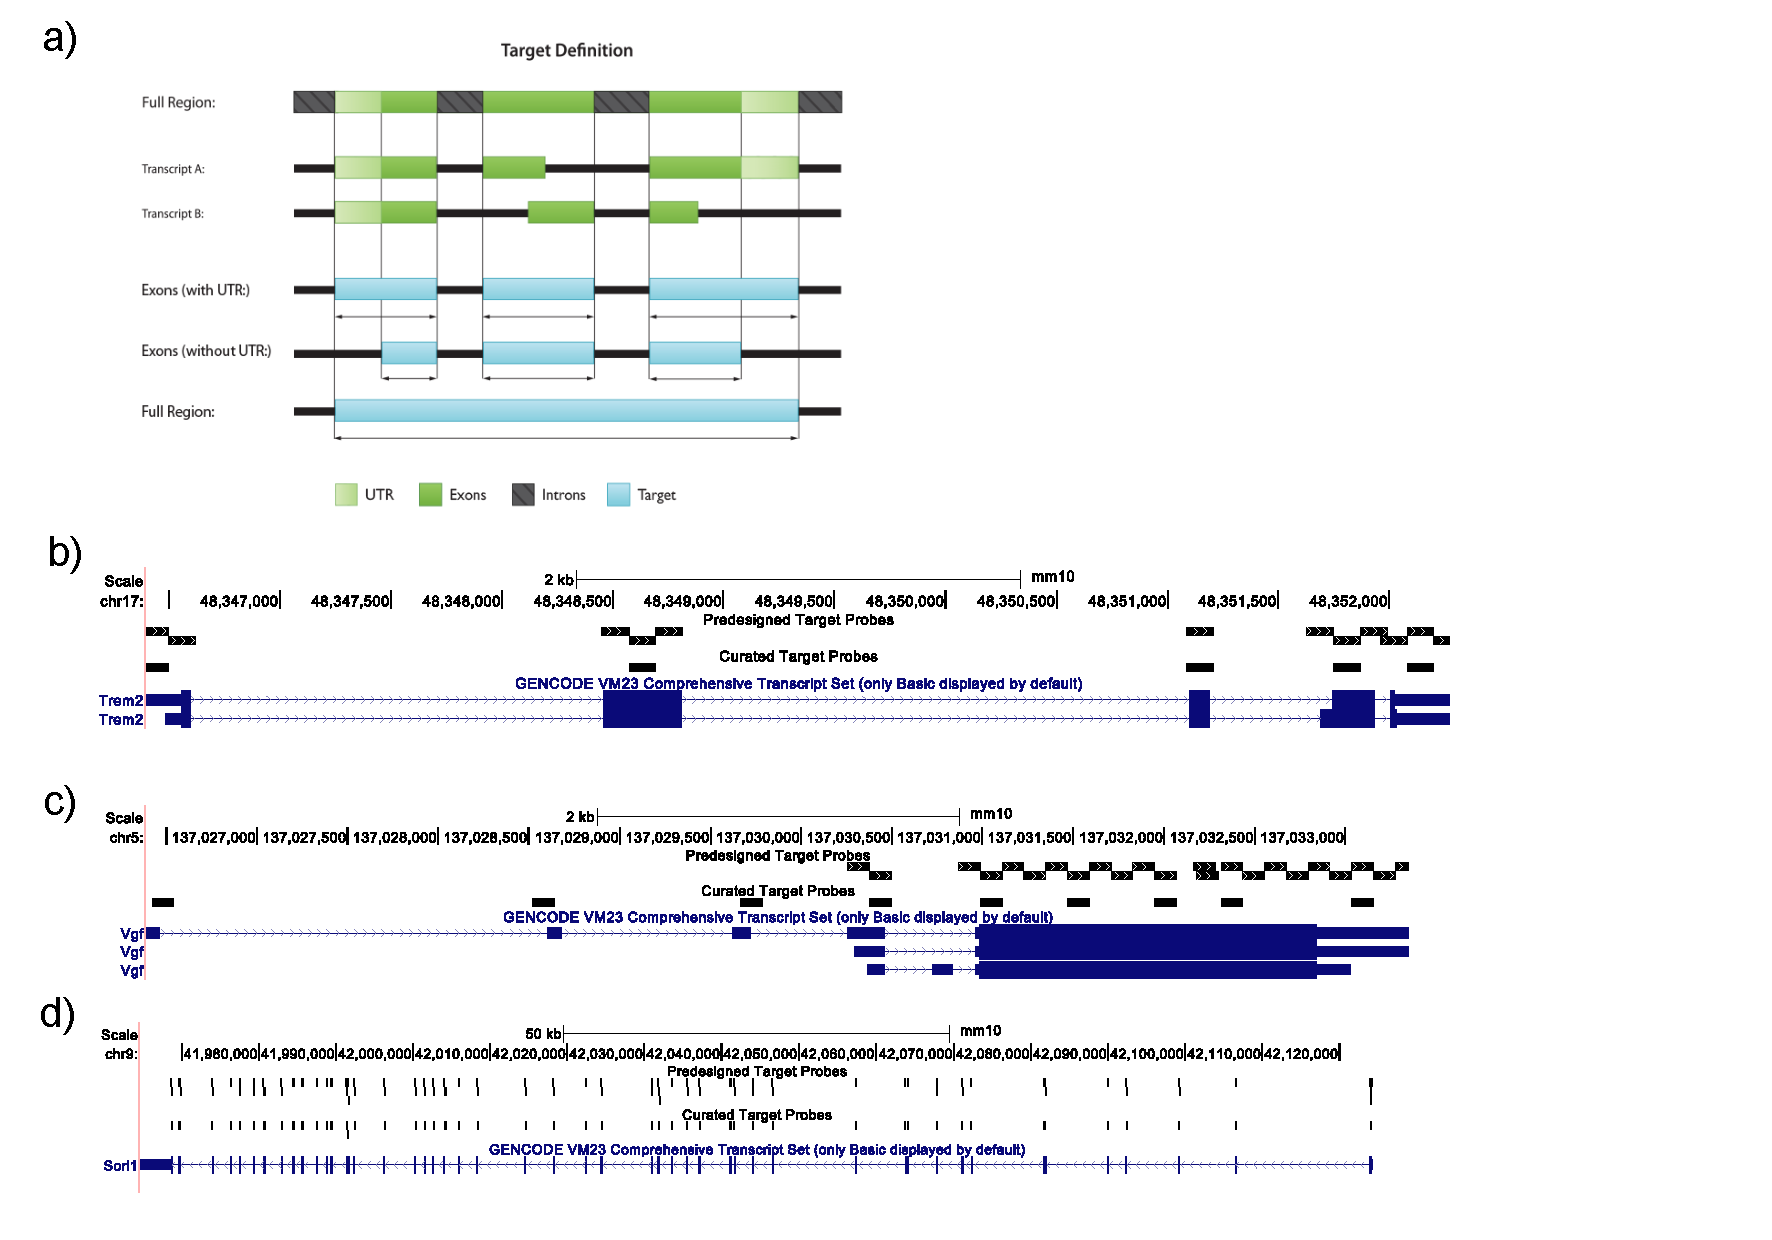
\includegraphics[page=1,trim={0cm 10cm 0cm 0cm},clip,scale = 0.90]{Figures/TargetProbes_Visualisation.pdf}
		\end{center}
		\captionsetup{width=1.5\textwidth}
		\caption[Manual curation of probes designed to 20 AD-associated target genes]%
		{\textbf{Manual curation of probes designed to 20 AD-associated target genes.} \textbf{A)} Pre-designed set of probes were provided to "Exons (with UTR)" of target genes. Shown are USCS genome browser tracks of pre-designed and curated probes to \textbf{B)} \textit{Trem2}, \textbf{C)}\textit{Vgf} and \textbf{D)}\textit{Sorl1} in the mouse genome (mm10). As shown, exons were unnecessarily covered by contiguous probes which not only increases costs but also induces off-target binding (referred in figure as "Pre-designed Target Probes"). Manual curation was therefore needed for each target gene (referred in figure as "Curated Target Probes") to ensure that exons were covered with one probe for every 500bp. }
		\label{fig:target_probes_eg}
	\end{figure}
\end{landscape}

\subsubsection{Library Preparation, Primer Annealing \& Polymerase Binding}
\label{section:ch2_smrtbelltemplate_explanation} 
After equimolar pooling the two fractions for global transcriptome profiling and/or multiple samples for targeted transcriptome profiling (\cref{section:ch2_ampurebead_pool}), SMRTbell template preparation was performed with the SMRTbell Template Prep Kit v1.0 (PacBio). This first involved repairing DNA damage and polishing ends of fragments (\cref{fig:isoseq_labworkflow}, Step 1, 2), essential for the generation of high-quality library of closed, continuous and circular SMRTbell templates. Abasic sites were filled, thymine dimers resolved, and deaminated cytosine alkylated. 3’ overhangs were removed, whereas 5’ overhangs were filled-in by T4 DNA Polymerase and phosphorylated by T4 PNK for ligation of blunt hairpin adapters. Following 1X AMPure bead purification of repaired dsDNA, hairpin adapters were ligated to the blunt ends for 24hours (\cref{fig:isoseq_labworkflow}, Step 3). Any templates failing to ligate were removed with exonuclease III and VII (\cref{fig:isoseq_labworkflow}, Step 4). The repaired, ligated SMRTbell library was then purified with two rounds of 1X AMPure beads, and assessed for quality and quantity with Qubit and Bioanalyzer assays before proceeding to primer annealing and polymerase binding (\cref{fig:isoseq_labworkflow}, Step 5, 6). Of note, the primer and polymerase to template ratio was key to successful loading of SMRTbell templates into ZMWs for sequencing, and was dependent on the final library molarity (as determined using \textbf{Equation \ref{eqn:isoseq_library_molarity}}). 


\subsubsection{Loading and Sequencing} 
\label{section:ch2_sequencing}
All Iso-Seq experiments in this thesis were performed on the PacBio Sequel 1M SMRT cell. Samples were processed using either the v3 chemistry (Diffusion Loading at 5pM with a 4-hour pre-extension and a 20-hour capture time) or v2.1 chemistry (Magbead Loading at 50pM with a 2-hour pre-extension and 10-hour capture time). All the samples bar the first two were sequenced using Diffusion Loading. As suggested in the name, Diffusion Loading involved immobilising polymerase-bound SMRTbell templates to ZMW by diffusion, whereas Magbead loading using paramagnetic beads ("Magbeads") that rolled across the ZMWs. Due to the different nature of loading, Diffusion Loading preferentially loads shorter transcripts, whereas Magbead Loading preferentially loads longer transcripts (>1b). For quality-control measure of loading and sequencing performance, a DNA Internal Control Complex (PacBio) was added to each library before sequencing, the amount of which was dependent on the final library molarity. Mimicking SMRTbell templates, this Internal Control is composed of a 1966bp-insert with the SMRTbell adapters already ligated and the  polymerase bound.


\begin{figure}[!htp]
	\begin{center}
		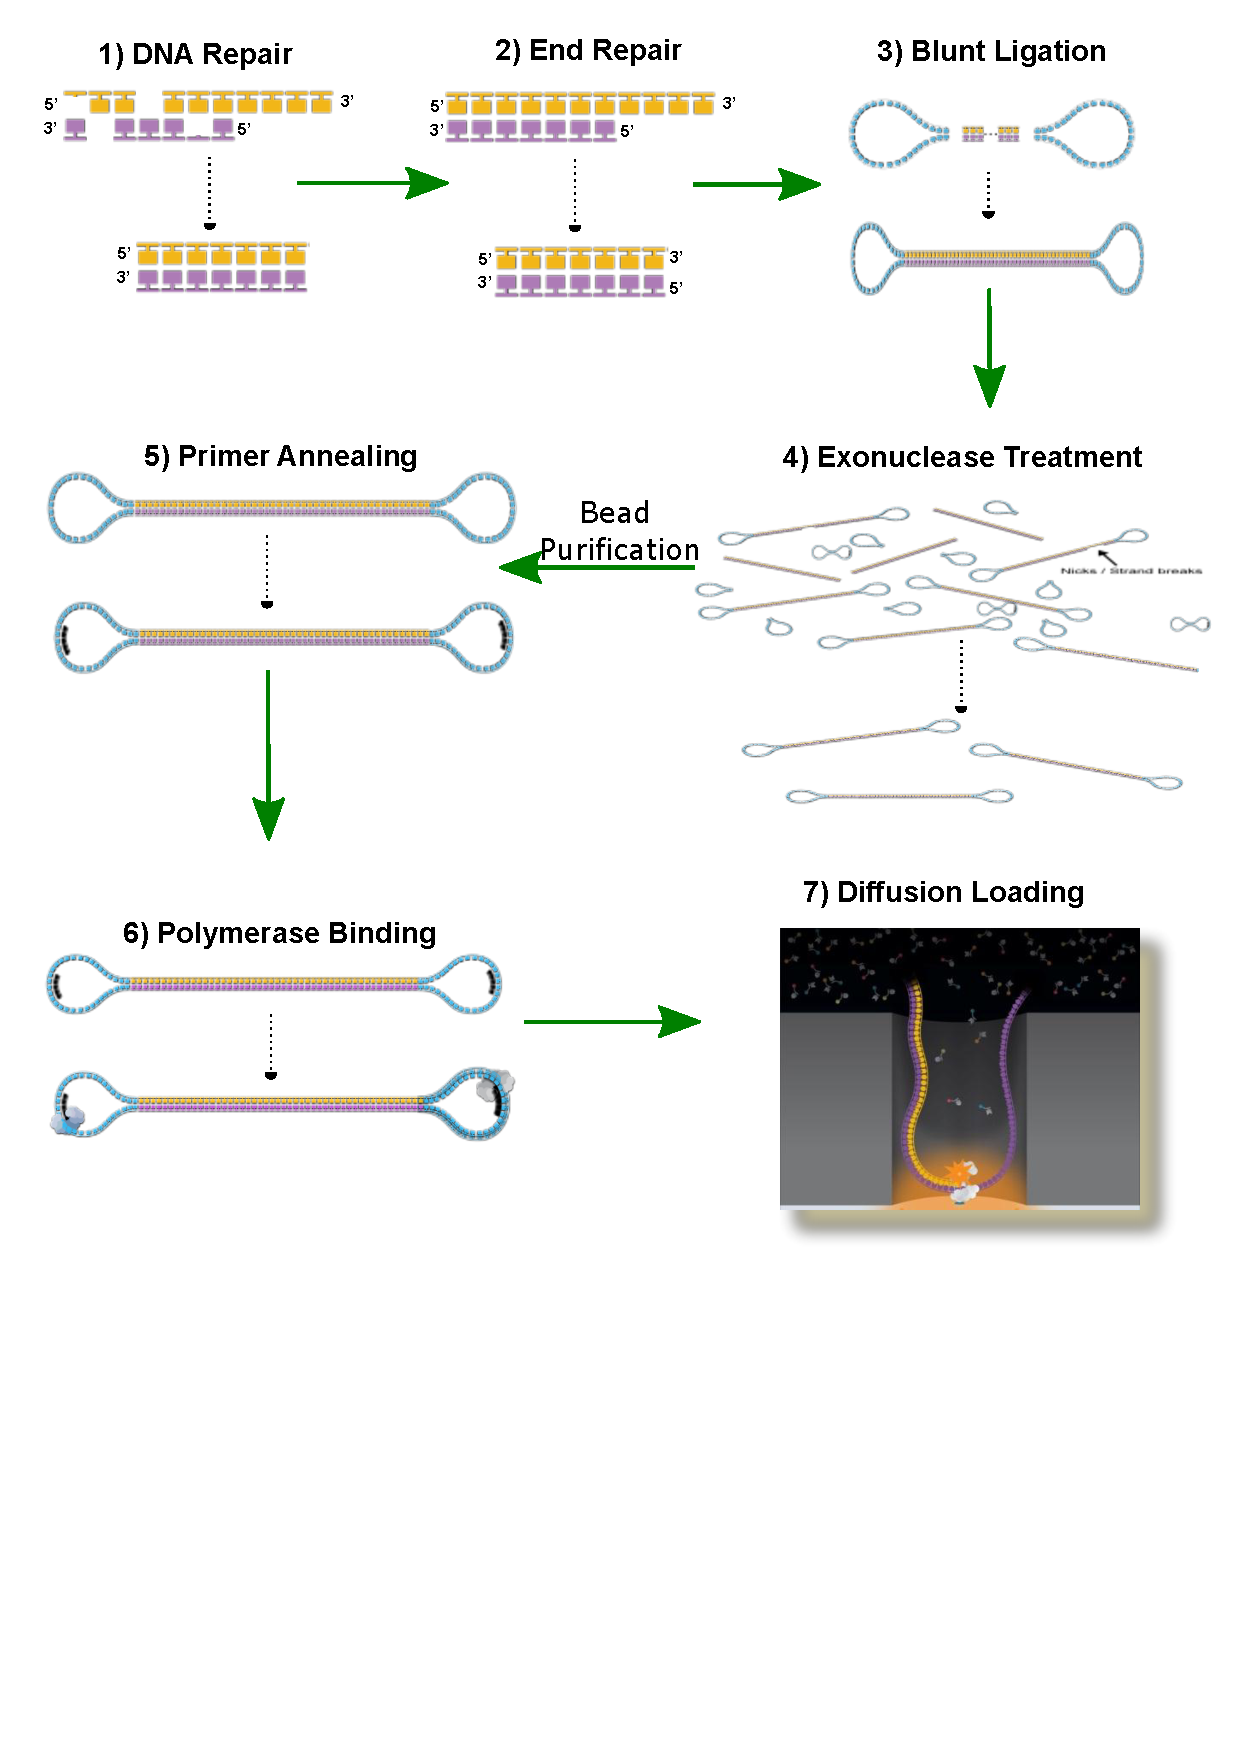
\includegraphics[page=1,trim={0cm 8cm 0cm 0cm},clip,scale = 0.70]{Figures/labwork_isoseq.pdf}
	\end{center}
	\captionsetup{width=0.95\textwidth,singlelinecheck=off}
	\caption[Iso-Seq Lab workflow for SMRTbell Template Preparation, Primer Annealing \& Polymerase Binding]%
	{\textbf{Iso-Seq Lab workflow for SMRTbell Template Preparation, Primer Annealing \& Polymerase Binding.} Shown is a flow diagram of the Iso-Seq lab workflow for library preparation:
		\begin{enumerate}
			\item Repair DNA by filling in abasic sites, removing thymine dimers, oxidising guanines, deaminating cytosine. This is essential to ensure a continuous sequence for uninterrupted polymerase processivity.
			\item Repair ends for blunt ligation with removal of 3'hangs and addition of 5'hangs by T4 DNA polymerase, which is required for blunt ligation of SMRTbell adapters. 
			\item Blunt Ligation by adding hairpin SMRTbell adapters to repaired ends
			\item Exonuclease treatment to remove incomplete SMRTbell templates with Exonuclease III and IV to ensure optimal sequencing
			\item Annealing of primers to both ends of the SMRTbell templates to initiate sequencing 
			\item Binding of polymerase to both ends of SMRTbell templates for efficient loading into ZMWs
			\item Immobilisation of polymerase-bound SMRTbell templates to ZMW by diffusion
			\\
		\end{enumerate} 
		Individual figures and legend are taken and adapted from "PacBio Sequel Library and Sequencing Preparation" presentation
	}
	\label{fig:isoseq_labworkflow}
\end{figure}

\clearpage
\subsection{Run Performance and Quality Metric}
\label{sec: Isoseq_run_performance}
Suboptimal PacBio sequencing performance could be due to various reasons from potential issues with the instrument and sequencing reagents to poor library preparation and incorrect loading. The performance of a sequencing run can be assessed by the performance of the DNA Internal Control and productivity metrics. 

\boldheader{DNA Internal Control} 
Sequencing metrics for the DNA Internal Control (described in \cref{section:ch2_sequencing}) is provided in several ways: i) the number of control reads, ii) the mean control polymerase read length, and iii) the proportion of sequence identity match between the control raw reads and the reference control (concordance). Short control read lengths and/or low control read counts are suggestive of issues with the PacBio instrument and consumables, while a low concordance value (< 0.84) indicate overloading of SMRT cells. Conversely, normal control sequencing metrics in a run with overall low yield indicate sample-specific issues. The expected sequencing metrics from a correctly prepared control in a good Iso-Seq sequencing run are documented in \cref{tab:control_Isoseqmetrics}. 

\vspace{1cm}
\begin{table}[!h]
	\caption[Iso-Seq DNA Internal Control Sequencing Metrics]%
	{\textbf{Iso-Seq DNA Internal Control Sequencing Metrics.} Tabulated are the expected median values for the number of control reads (median count), the control polymerase read length (median length), and the identity match between control raw reads and reference sequence (median concordance). The expected values provided assume a sequencing run performed on the PacBio Sequel 1M SMRT cell with a 4-hour pre-extension and a 20-hour capture time. QR - Quantile range.}	\label{tab:control_Isoseqmetrics}
	
	\centering
	\begin{tabular}{@{}cccc@{}}
		\toprule
		Metrics         & Median Count (QR)     & Median Length (kb) (QR) & Median Concordance (QR) \\ \midrule
		Expected Values & 6900 (4,000 - 10,200) & 46.9 (41.5 – 52.5) & 0.862 (0.857 – 0.867)   \\ \bottomrule
	\end{tabular}
\end{table}


\boldheader{Productivity Metrics} 
Productivity or loading metrics is a measure of the number of ZMWs that generated a positive signal that was then translated into useful sequencing data. Each ZMW is classified as either: 
\begin{itemize}
	\item P0 (Productivity 0): no active sequencing polymerase complex with no signal 
	\item P1 (Productivity 1): productive ZMWs with a high quality (HQ)\nomenclature{HQ}{High quality} region* within read 
	\item P2 (Productivity 2): detectable signal but no HQ region* detected, possibly due to overloading of multiple inserts with multiple polymerases
\end{itemize}
*HQ region is defined as a high quality sequence of >50bases.   

An optimal sequencing run is indicated by achieving a total run yield of 20-30Gb with \textasciitilde70\% of ZWMs in P1 (positive signal), and 20-30\% ZMWs in P0 (empty ZMWs). A low P0 (<20\%) indicates over-loading of polymerase-bound templates, resulting in shorter P1 polymerase reads and poor sequencing yield (noisy base-calling). Conversely, a high P0 (>40\%) from under-loading would generate fewer P1 reads and result in low sequencing yield. A combination of high P0, low P1 and high P2 loading profiles indicates presence of contaminants (possibly from poor AMPure bead purification) that is interfering with productive polymerase activity. A good balance between P0, P1 and P2 is therefore key to achieving a good sequencing run with high yield and high-quality, long P1 polymerase reads. Multiple titrations of loading concentrations can be trialled to determine the optimum loading concentration essential for reaching this balance. 

\clearpage
\subsection{Bioinformatics Pipeline} 
\label{section:isoseq_bioinformatics}
This section describes the bioinformatics pipeline for analysing Iso-Seq data generated on the PacBio Sequel I following Iso-Seq library preparation (\textbf{Chapters 4 - 6}). 

The bioinformatics pipeline, as depicted in \cref{fig:isoseq_bioinformatics_Pipeline}, involved three main steps: i) processing and filtering of raw reads to generate HQ, full-length transcripts using the PacBio \textit{IsoSeq3} suite \cite{Gordon2015}, ii) alignment of HQ transcripts to the reference genome using \textit{Minimap2}\cite{Li2018}, and iii) clustering and collapsing of mapped transcripts to unique, annotated isoforms using \textit{Cupcake}\cite{TsengCupcake} and \textit{SQANTI}\cite{Tardaguila2018}. Public annotations and short-read RNA-Seq data were used for validating Iso-Seq derived isoforms. 

While Iso-Seq raw data can be processed using the PacBio SMRT Link Suite, a web-based end-to-end user interface, we developed an end-to-end command line that allowed simultaneous parallel processing of multiple samples and streamlining of the analysis after raw read processing. The choice of parameters and packages were guided by a separate analysis on external RNA Spike-In controls (ERCC) that were sequenced within the same runs (described in \cref{section:ch2_ERCC_explanation}). 

\begingroup
\parindent=0em
\etocsettocstyle{\rule{\linewidth}{\tocrulewidth}\vskip0.5\baselineskip}{\rule{\linewidth}{\tocrulewidth}}
\etocsetnexttocdepth{5}
\localtableofcontents 
\endgroup


\begin{figure}[]
	\centering
	\vspace{20pt}
	\includegraphics[page=17,trim={0 6cm 0 0},clip,scale = 0.8]{Figures/ProjectDevelopment_Figures.pdf}
	\captionsetup{width=0.95\textwidth}
	\caption[Iso-Seq Bioinformatics Pipeline]%
	{\textbf{Iso-Seq Bioinformatics Pipeline.} Shown is an overview of the Iso-Seq bioinformatics pipeline, which primarily involves three main steps: i) processing and filtering of raw reads into high-quality, full-length transcripts using \textit{IsoSeq3}, ii) alignment of HQ transcripts to the reference genome using \textit{Minimap2} and iii) collapsing of mapped transcripts to unique, annotated isoforms using \textit{Cupcake} and \textit{SQANTI}. HQ - High quality}
	\label{fig:isoseq_bioinformatics_Pipeline}
\end{figure}

\clearpage
\subsubsection{Processing of Iso-Seq raw reads}
\label{section: Isoseq_rawprocessing}
In response to a much higher experimental throughput of the PacBio Sequel compared to the older PacBio RSII sequencer, the official PacBio bioinformatics suite for processing Iso-Seq reads (henceforth referred to as \textit{Iso-Seq3}) has been revised multiple times over the course of this research. Each subsequent version delivered a reduction in runtime coupled with an improvement in sensitivity and specificity to recover transcripts and reduce artefacts. A particularly noteworthy development was the forgoing of non-FL reads or RNA-Seq short-reads for error correction, due to the high throughput and subsequent generation of high-quality, accurate Iso-Seq reads. 

Despite multiple major updates to \textit{Iso-Seq3}, the core principles and processing steps have remained the same (depicted in \cref{fig:isoseq3_tool}), namely: i) the generation of CCS reads from each sequencing ZMW, ii) identification of FL reads with removal of cDNA primer and poly(A) tail, and iii) grouping of FL reads derived from the same transcript. 

\boldheader{Generation of CCS reads with \textit{CCS}}
Raw Iso-Seq subreads from each productive ZMW were processed to generate one representative circular consensus read (\cref{fig:isoseq3_tool}\textbf{A, B}) using \textit{CCS} (v5.0.0) with the following parameters: 
\begin{itemize}
	\item minimum number of full "passes" for a ZMW to be considered. A full pass is defined by the presence of both SMRT adapters at both ends (default: 3 passes)
	\item minimum predicted read accuracy across all subreads (default: 99\%)
	\item minimum and maximum length of subreads to generate a CCS (default: 10 and 21000 bases, respectively)
	\item quality of subreads predicted by the CCS model (default: -3.5 Z-score), and proportion of total subreads meeting the quality score (default: \textgreater 30\%)
\end{itemize}

%Across literature and PacBio scientific community, different parameter settings were recommended, particularly with \textit{number of full passes} and \textit{minimum base accuracy}, which had the greatest effect on the number of CCS reads generated for downstream analyses. Taking a subset of raw data from 10 randomised samples, a range of values across these two parameters were tested. CCS were then classified to full-length (FL, determined by the presence of 3'/5' primers and poly-A tail) and non-full-length (NFL) reads. 

\boldheader{Removal of primers and barcodes with \textit{Lima}}
After the successful generation of CCS reads, cDNA primers were identified and removed using \textit{Lima} (v2.0.0) to generate FL reads (\cref{fig:isoseq3_tool}\textbf{C}); additional barcode sequences were also included for targeted sequencing experiments to perform sample demultiplexing. Sequences were then orientated from 5’ to 3’, and any reads with unwanted combinations were removed. Of note, the ratio of recovered FL reads to CCS reads varied on the insert transcript size, but a good sequencing library with a distribution of 1-3kB was estimated to recover 60-70\% of CCS reads as FL reads.   

\boldheader{Trimming of poly(A) tails and concatemer removal with \textit{Refine}}
FL reads were further refined by the trimming of poly(A) tails (with a minimum length of 20 adenosine bases), and removal of artificial concatemers to generate full-length non-chimeric (FLNC\nomenclature{FLNC}{Full-length non-chimeric} reads (\cref{fig:isoseq3_tool}\textbf{D}). Artificial concatemers are cDNA sequences with internal runs of poly(A) and poly(T) sequences that are generated from using insufficient amount of blunt adapters during library preparation. The occurrence of these artefacts should be low (<0.5\%) in a standard library preparation, and the number of FLNC reads and FL reads should be similar. Any significant loss of reads at this stage implicates issues with SMRTbell library preparation.

\boldheader{Grouping of reads into transcripts with \textit{Cluster}}
Using an iterative isoform-clustering algorithm, two or more FLNC reads were considered to be the same transcript, if the reads: 
\begin{itemize}
	\item differed < 100bp on the 5’ end* 
	\item differed < 30bp on the 3’end 
	\item do not contain internal gaps with >10bp
\end{itemize}
* Greater leeway was given to the 5'end than the 3'end to account for 5' RNA degradation

A minimum of two FLNC reads was required for clustering with the longest read chosen as the representative transcript, and any unique FLNC read failing to cluster were discarded (\cref{fig:isoseq3_tool}\textbf{E}). Transcripts generated from the \textit{Iso-Seq Cluster} were therefore high quality with a consensus accuracy $\geq$99\% and a minimum of 2 FLNC read support (\cref{fig:isoseq3_tool}\textbf{F}). 

\begin{figure}[htp]
	\centering
	\includegraphics[page=18,trim={0 8cm 0 0},clip,scale = 0.8]{Figures/ProjectDevelopment_Figures.pdf}
	\captionsetup{width=0.95\textwidth, singlelinecheck=off}
	\caption[PacBio \textit{Iso-Seq3} Bioinformatics suite for raw Iso-Seq read processing]%
	{\textbf{PacBio \textit{Iso-Seq3} Bioinformatics suite for raw Iso-Seq read processing}: An overview and flow diagram of \textit{Iso-Seq3} Bioinformatics suite. \textbf{A)} The circular SMRTbell template allows uninterrupted, processive DNA synthesis to generate a polymerase read containing multiple subreads. \textbf{B)} \textit{CCS} - A polymerase read, associated with each productive ZMW, with multiple "passes" are processed to generate a CCS read containing the 5' and 3' cDNA primer, polyA tail and barcode (if used). \textbf{C)} \textit{Lima} - Successfully generated CCS reads are then trimmed for cDNA primers and orientated to generate FL reads. \textbf{D)} \textit{Refine} - FL reads are then trimmed for poly(A) tails and artificial concatemers are removed to generate FLNC reads. \textbf{E)} \textit{Cluster} - FLNC reads considered to be derived from the same transcript are then clustered to generate unique transcripts. \textbf{F)} The output from this pipeline is the processing of raw Iso-Seq reads to accurate, high quality transcripts without the need for a reference genome or transcriptome. Of note, the abundance for each transcript can be inferred from the number of associated FL reads (i.e number of ZMWs that sequenced the isoform of interest). CCS - Circular consensus sequence, FL- Full-length, FLNC - Full-length Non-chimeric.}
	\label{fig:isoseq3_tool}
\end{figure}

\newpage
\subsubsection{Alignment to reference genome} 
HQ-transcripts generated from \textit{IsoSeq3} package were then aligned to the reference genome using \textit{Minimap2}\cite{Li2018} (v2.17), a splice-aware aligner that is faster, more precise and accurate than other mainstream mappers \cite{SimirKriZanoviC2018,Tang2020}. Under the recommended parameters ("-ax splice -uf --secondary=no -C5 -O6,24 -B4”), \textit{Minimap2} prioritises the known canonical junctions (GT[A/G]…[C/T]AG) over non-canonical splice junctions (GT[C/T]…[A/G]AG), and assumes that read orientation is unknown in order to perform two rounds of alignment which slightly improves accuracy. 

\subsubsection{Further transcript collapse to isoforms using \textit{Cupcake}}
Aligned HQ-transcripts were filtered and further collapsed to unique, full-length, high-quality isoforms using a set of supporting scripts from \textit{Cupcake} to reduce redundancy. Using the \textit{collapse\_isoforms\_by\_sam.py} script (parameters: "-c 85 -i 95 --dun-merge-5-shorter"), aligned transcripts with less than 85\% coverage and 95\% identity to the reference genome were removed. The number of associated FL reads associated with each isoform was then obtained as a proxy of isoform abundance with \textit{get\_abundance\_post\_collapse.py} script. 

\subsubsection{Transcriptome annotation with \textit{SQANTI}}
\label{section: sqanti_annotations}
Isoforms were characterised using SQANTI\cite{Tardaguila2018} (v3) which i) performs a reference-based correction of sequences, ii) classifies isoforms based on splice junctions, iii) annotates the transcriptome with user-defined public annotations and matched RNA-Seq data, and iv) discard isoforms that are considered technical artefacts. 

\boldheader{Isoform classification by splice junctions}
Isoforms can be broadly classified as either known or novel and annotated to a known gene, or novel and annotated to a novel gene not currently annotated in existing genome annotations. Using \textit{SQANTI}, known isoforms annotated to known genes were subclassified as Full Splice Match (FSM\nomenclature{FSM}{Full Splice Match}) if it fully aligned with the reference isoform with the same exonic structure and splice junctions, or Incomplete Splice Match (ISM\nomenclature{ISM}{Incomplete Splice Match}) if it has fewer 5’ exons than the reference isoform but is otherwise fully matching. Conversely, novel isoforms annotated to novel genes were subclassified as Novel in Catalogue (NIC\nomenclature{NIC}{Novel in Catalogue}) if it contained a different exonic structure with a combination of known donor or acceptor sites, or Novel Not in Catalogue (NNC\nomenclature{NNC}{Novel Not in Catalogue}) if there is at least one novel donor or acceptor site. Finally, novel isoforms from novel genes were subclassified as either antisense or intergenic depending on the orientation. Depictions of RNA isoform classifications can be found in \cref{fig:sqanti_cate}. Splice junctions were defined by the two pairs of dinucleotides present at the exon-intron boundary, and any other combinations aside from GT-AG, GC-AG and AT-AC pairs were considered non-canonical. 

Isoforms were also classified as protein-coding, using the GeneMarkS-T algorithm \cite{Tang2015}, if there is an open reading frame (ORF) with AUG as the initial codon. For incomplete isoforms (ISMs) with shortened 5'end, ORF was predicted from the first in-frame methionine. An isoform was predicted to undergo nonsense mediated decay if there is a predicted ORF and the coding sequence (CDS) ends at least 50bp from the last junction. 

\boldheader{Usage of public annotations and matched RNA-Seq data}
Various public annotations were supplied into \textit{SQANTI} for deeper characterisation of the transcriptome, including:
\begin{itemize}
	\item Cap Analysis of Gene Expression (CAGE) Peak from FANTOM5 dataset \cite{Lizio2019}, which map transcripts, transcription factors, transcriptional promoters and enhancers
	\item Intropolis junction bed file\cite{Nellore2016} from a comprehensive human RNA-Seq dataset
	\item Human and mouse poly(A) motifs provided by \textit{SQANTI}	 
\end{itemize}

Matched RNA-Seq data was also supplied to \textit{SQANTI} in two forms: i) after alignment to reference genome using \textit{STAR}\cite{Dobin2013} (v1.9) to infer the number of RNA-Seq reads at splice junctions, and ii) alignment to Iso-Seq-derived aligned transcripts using \textit{Kallisto}\cite{Bray2016} (v0.46.0) for RNA-Seq expression.  

\begin{landscape}
	\begin{figure}[h]
		\centering
		\includegraphics[page=3,trim={0 4cm 0 0},clip,scale = 0.9]{Figures/ProjectDevelopment_Figures_Landscape}
		\captionsetup{width=1.5\textwidth}
		\caption[Isoform Classifications by \textit{SQANTI}]%
		{\textbf{Isoform Classifications by \textit{SQANTI}}. Isoforms were classified by \textit{SQANTI} as novel or known, and annotated to novel or known genes based on splice junctions}
		\label{fig:sqanti_cate}
	\end{figure}
\end{landscape}

\boldheader{Further filtering for technical artefacts}
\textit{SQANTI Filter} was used to filter the curated transcriptome for any technical artefacts that were generated during library preparation, namely: i) RT template-switching events, which occur when RT transits within or across DNA templates without terminating cDNA synthesis, particularly if the original DNA template harbours two or more direct repeats\cite{Cocquet2006} (\cref{fig:lib_prep_artifacts}\textbf{A}), and ii) off-priming events when oligo(dT) primer binds to other internal homo-polymeric adenines (A) regions located within the cDNA template\cite{Conesa2016} (\cref{fig:lib_prep_artifacts}\textbf{B}). These events can generate chimeric or short, incomplete, truncated cDNA that can otherwise be misinterpreted as isoforms generated from non-canonical splicing\cite{Houseley2010}. 

It was therefore pertinent to perform additional filtering using \textit{SQANTI}, which identified RT-switch events by searching for direct repeats (given that RT switching is homology dependent) and intra-priming events by removing isoforms with >60\% of adenosines (A) within the 20-nucleotide window in the genome downstream of the isoform TTS; a lower proportion of genomic As after the TTS referred to a lower likelihood of poly(A) tail being present and greater likelihood for off-priming. 

\begin{figure}[h]
	\begin{center}
		\includegraphics[page=4,trim={2cm 21.5cm 0 1cm},clip, scale = 0.9]{Figures/ProjectDevelopment_Figures.pdf}
	\end{center}
	\captionsetup{width=0.95\textwidth}
	\caption[Generation of technical artefacts during cDNA synthesis]%
	{\textbf{Generation of technical artefacts during cDNA synthesis. A)}: shown is a schematic diagram of reverse transcription template-switching. The black and blue lines represent the original cDNA and synthesising cDNA from RT, respectively. The black box and light grey sphere represent the direct repeats and RT enzyme, respectively. As exemplified, RT template switching is further facilitated by RNA secondary structures that could bring the repeats into proximity\cite{Cocquet2006}. Figure is taken from Cocquet et al.(2006)\cite{Cocquet2006}. \textbf{B)} Shown is a schematic diagram of off-priming events from priming of oligo(dT) to an internal poly(A) sequence rather than the 3'end poly(A) tail during cDNA synthesis, generating two truncated cDNA templates. Figure is taken from Nam et al.(2002)\cite{Nam2002}. }
	\label{fig:lib_prep_artifacts}
\end{figure}

Under these filtering criteria (depicted in \cref{fig:sqantifiltering}), an isoform classified as FSM was always retained unless the 3'end was unreliable (i.e. >50bp from reference TTS), implicating the occurrence of intra-priming events. Conversely, much more stringent filters were applied to other isoforms not classified as FSM, and such isoforms were only retained if the 3'end was reliable, if they did not contain a junction detected as RT switching and all the junctions were either canonical or supported by at least three RNA-Seq reads (if matched RNA-Seq data is provided).   

\begin{figure}[!h]
	\begin{center}
		\includegraphics[page=19,trim={0 12cm 0 0},clip, scale = 0.8]{Figures/ProjectDevelopment_Figures.pdf}
	\end{center}
	\captionsetup{width=0.95\textwidth}
	\caption[Filtering of technical library artefacts using \textit{SQANTI}]%
	{\textbf{Filtering of technical library artefacts using \textit{SQANTI}.} Shown is a binary decision tree for \textit{SQANTI Filter} of isoforms. An isoform classified as Full Splice Match (FSM) is always retained unless the 3'end is unreliable (i.e. no detected poly(A) motif and >50bp from reference TTS). Conversely, all the other classified isoforms are only retained if the 3'end is reliable, and do not contain any junctions that are either predicted RT switching or are not supported by matched RNA-Seq data. Coloured boxes indicate the output from decision tree with red and green box indicating isoforms being removed and retained, respectively.}
	\label{fig:sqantifiltering}
\end{figure}

\subsubsection{Usage of ERCC to inform Iso-Seq bioinformatic analysis}
A set of 92 synthetic spike-in controls, ERCC, was added to the global transcriptome profiling experiments (described in \cref{section:ch2_ERCC_explanation}) to assess the sensitivity of the Iso-Seq approach and guide the downstream bioinformatics pipeline. After processing of Iso-Seq raw reads (described in \cref{section: Isoseq_rawprocessing}), HQ-transcripts were aligned to ERCC reference sequences in parallel to the reference genome, followed by collapsed using \textit{Cupcake} scripts under default parameters (-c 95 -i 99) and \textit{SQANTI} annotations - the standard bioinformatics pipeline that has been recommended by the PacBio research community. 

Application of this pipeline, however, only detected over a third of ERCC molecules (n = 37, 40.22\%) with several annotated with more than one isoform (n = 8, 8.7\%), contrary to the fact that there should only be one synthetic molecule sequenced for each ERCC. These "multiple-isoformic ERCC" were known to be more abundant, suggesting that more highly-expressed genes are likely to be associated with more isoforms that have failed to collapse properly. Visualisation and BLAST analysis of these "isoforms" revealed them to be shorter fragments of the original ERCC sequence, generated as technical artefacts either from fragmentation of the originals molecule or incomplete PCR synthesis. Application of \textit{Tama-remove-fragment-models.py} script from \textit{TAMA}\cite{Kuo2017} successfully removed these partial, redundant isoforms, while retaining the longer, intact isoforms. 

Deeper investigation into the low coverage of ERCC identified an additional 20 less-abundant ERCC molecules that were 
discarded from \textit{Cupcake} due to an imperfect reference alignment with a shorter 5'end, a likely result of 5'degradation. Lowering the coverage threshold from 99\% (default) to 95\% rescued these ERCC molecules and increased the total number of ERCC molecules detected by 20\% (unique number of ERCC = 57, 61.96\%), subsequently strengthening the correlation between FL Iso-Seq read count and the actual amount of ERCC used (95\% coverage: corr = 0.98, p = 1.41 x 10\textsuperscript{-41}; 99\% coverage: corr = 0.82, p = 4.89 x 10\textsuperscript{-10}). Notably, this finding highlights the limitation of our current Iso-Seq approach in failing to i) differentiate between intact and truncated RNA in our cDNA synthesis kit, resulting in our lack of confidence on isoform TSS, and ii) detect lowly-expressed genes and transcripts (coverage) where the deleterious impact of RNA degradation is even more significant. 

\clearpage

\section{Oxford Nanopore Technologies: cDNA Sequencing}
\label{sec:ONT_cDNA_Sequencing}
%https://www.nature.com/articles/s41587-020-0731-9

\subsection{Introduction}
Following the success of PacBio's SMRT for generating long sequencing reads in real-time (reviewed in \cref{tab: longread_isoseqstudies}), Oxford Nanopore Technologies (ONT) introduced an alternative long-read, single-molecule sequencing technology with the commercial release of the MinION in 2014. In contrast to all existing sequencing applications which rely on a "sequencing-by-synthesis" approach (including PacBio's SMRT sequencing), ONT technology pioneered the approach of directly reading a single DNA strand using a protein nanopore rather than by measuring incorporation events on the template strand\cite{Jain2015} (\cref{fig:ONT_Mechanism}\textbf{A}). Partly owing to the relatively lower cost and portability of ONT technology, nanopore sequencing has been widely used for transcriptome profiling (reviewed in \cref{tab: longread_ontstudies}), 
with theoretically no upper limit to read length \cite{Loman2015} (the longest read to date is over 150kb), and with no bias towards length or GC content \cite{Oikonomopoulos2016, Weirather2017}.


\subsubsection{Mechanism}
The MinION is a hand-held portable USB-powered device. At its centre is a flow cell that contains a sensor array, which houses a total of 2048 individual nanopores that are controlled in four groups of 512 channels; this allows up to 512 independent DNA molecules to be sequenced simultaneously\cite{Jain2015}. As a voltage is applied across the nanopore, the single-stranded DNA sequence translocates through the nanopore and subsequently interrupts the current in a nucleotide-dependent manner, generating a unique signal of electric current perturbations that acts as proxy of the underlying nucleotide sequence (\cref{fig:ONT_Mechanism}\textbf{A}). 

Successful nanopore sequencing requires the efficient capture and threading of ssDNA into the pore, followed by the ability to identify individual DNA bases in a time-resolved manner. This was achieved through several key innovations\cite{Bayley2015} 
\begin{enumerate}
	\item Generation of an internal positive charge within the protein nanopore to induce capture of negatively-charged DNA. Each nanopore is embedded into an electrical resistant membrane that is immersed in an electrolyte solution.
	\item Discovery and usage of biological pore proteins. The \textit{Staphylococcus aureus} \textit{α}HL pore was first implemented for sequencing\cite{N2005} followed by the \textit{Mycobacterium smegmatis} MspA pore\cite{Manrao2011}. Current ONT nanopore systems use a modified \textit{Escherichia coli} CsgG pore, containing a short and narrow channel constriction site, enabling detection of distinct ionic currents at a single-nucleotide resolution. 
	\item Ratcheting the DNA through the pore for time-resolved base identification with a processive enzyme (henceforth referred to as a motor protein, \cref{fig:ONT_Mechanism}\textbf{A,B}), which facilitates DNA movement and reduces the translocation speed of the molecule for improved signal (average speed of 450bp/s)\cite{Rang2018}. This processive enzyme is ligated to the 5'end of both strands during library preparation.   
\end{enumerate}

\begin{figure}[]
	\centering
	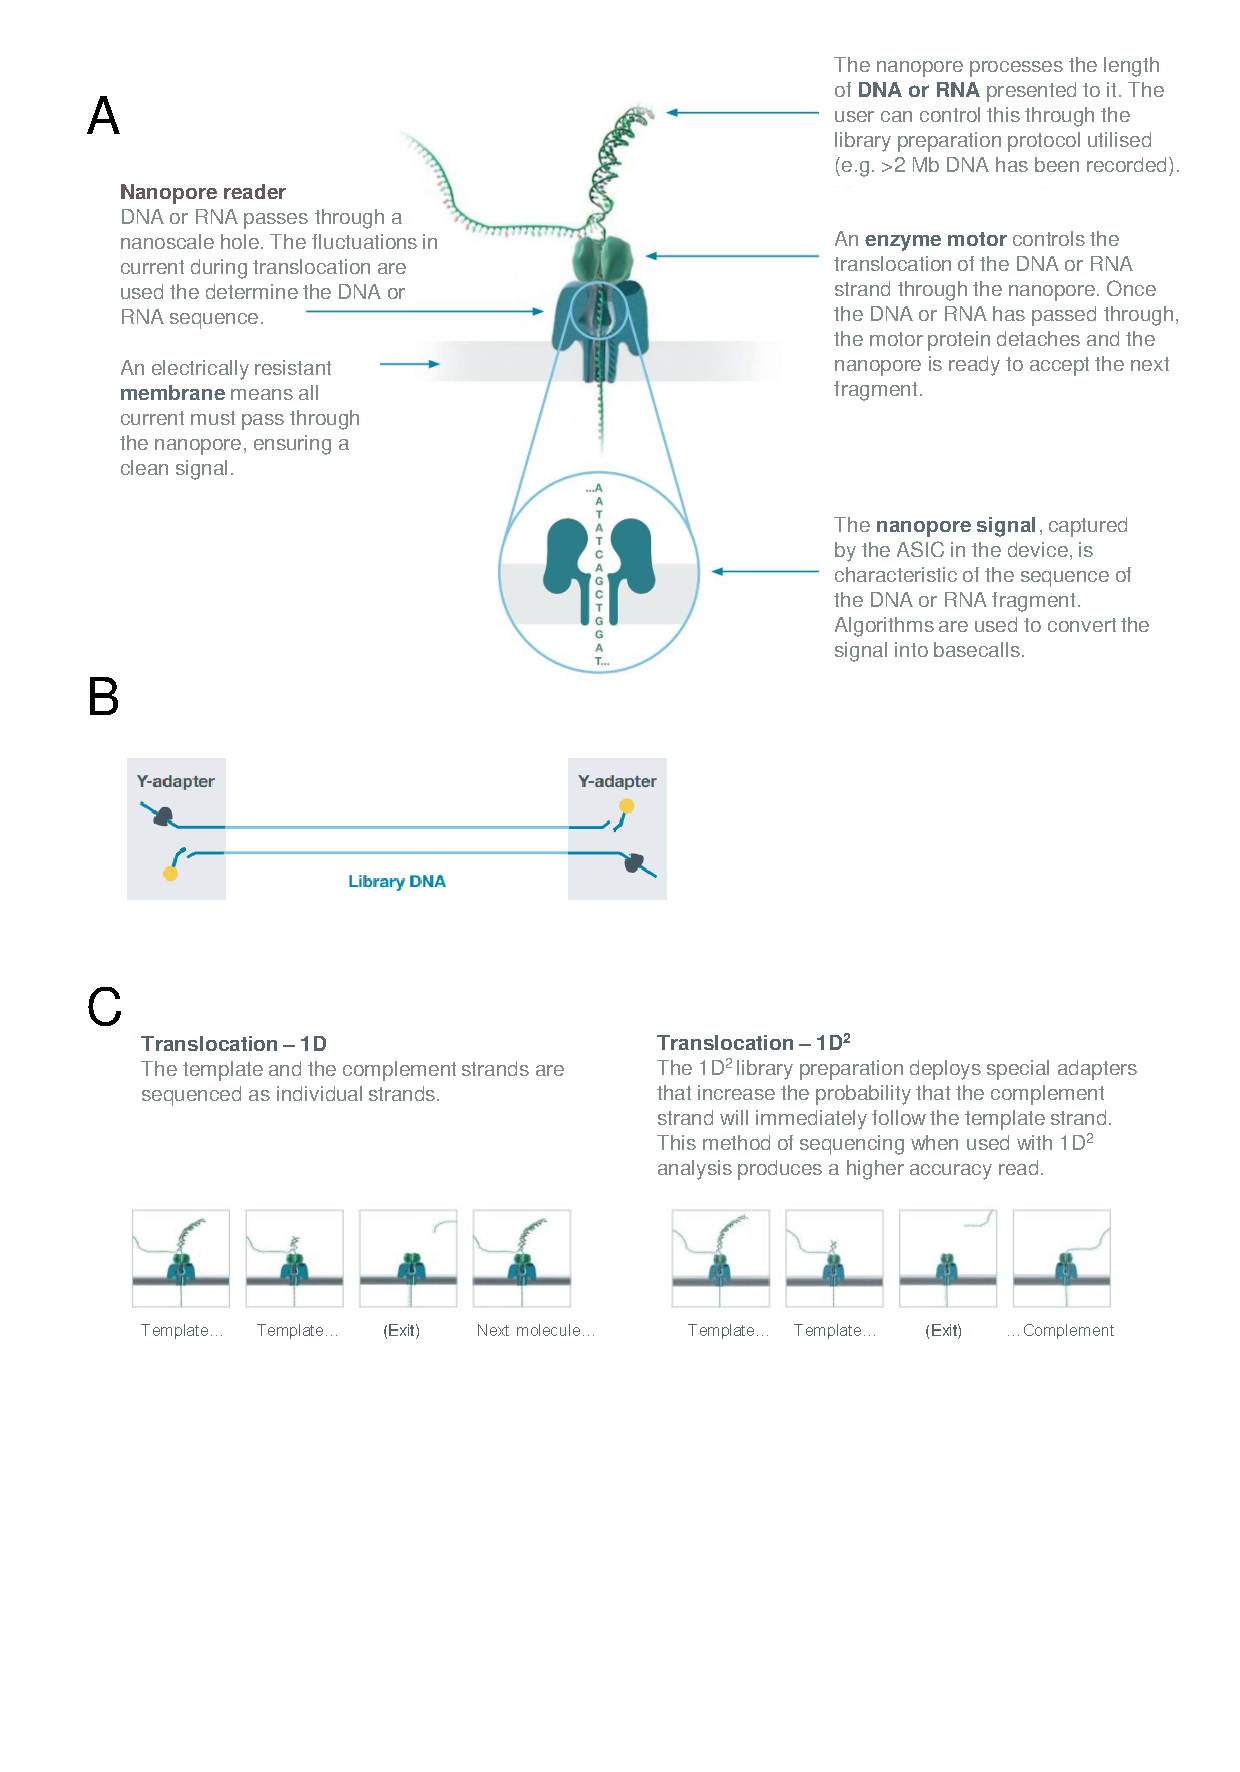
\includegraphics[page=1,trim={0 6cm 0 0 },clip, scale = 0.8]{Figures/ProjectDevelopment_FiguresONT}
	\captionsetup{width=0.95\textwidth}
	\caption[ONT nanopore cDNA Sequencing]%
	{\textbf{ONT nanopore cDNA Sequencing.} Shown is an overview of Oxford Nanopore Technologies (ONT) nanopore platform. \textbf{(A)} ONT nanopore sequencing involves the translocation of a DNA sequence through a biological nanopore, which is controlled by the enzyme motor protein and causes nucleotide-sensitive perturbations in the electric current. \textbf{(B)} The structure of the library DNA with ligation of the sequencing adapter, containing the motor protein (brown circle), to the template and complementary strand. \textbf{(C)} Two sequencing translocation modes are currently offered, generating either 1D or 1D\textsuperscript{2} reads. Figures are taken from Oxford Nanopore Product Brochure July 2018.}
	\label{fig:ONT_Mechanism}
\end{figure}

\clearpage
\subsection{Lab Workflow}
\label{chap:ont_labpipeline}
This section describes the library preparation for ONT cDNA sequencing experiments used in \textbf{Chapter 6} for the targeted transcriptome profiling of AD genes in the mouse cortex. At the time of my PhD research, the ONT technology was significantly less advanced that the PacBio technology with only basic protocols. Nanopore sequencing was therefore conducted on a subset of mouse samples as a source of validation and technology comparison using methods optimised during my research. 

For a fairer and more direct comparison, all steps prior to the ONT library preparation were adopted from the Iso-Seq protocol, including the conversion of RNA to cDNA using the SMARTer PCR cDNA synthesis (\cref{section:ch2_cDNA_synthesis_explanation}), large scale DNA amplification using the GXL DNA Polymerase and target enrichment with hybridisation-based capture (workflow is depicted in \cref{fig:ONT_TargetedProtocol}). Consequently, nanopore reads are generated with the same cDNA primers and barcode sequences as Iso-Seq reads (refer to \cref{tab:barcode_primers} for sequences). Post cDNA synthesis and amplification, the ONT library preparation is broadly similar to the Iso-Seq library preparation (also outlined in \cref{fig:ONT_TargetedProtocol}), with the exception that the motor enzyme is pre-bound to the adapters in ONT reads whereas the polymerase is only loaded after adapter ligation in Iso-Seq.  

\begin{figure}[]
	\centering
	\includegraphics[page=7,trim={0 6cm 0 0 },clip, scale = 0.7]{Figures/ProjectDevelopment_FiguresONT}
	\captionsetup{width=0.95\textwidth}
	\caption[Comparison of the ONT and Iso-Seq lab workflow for targeted profiling]%
	{\textbf{Comparison of the ONT and Iso-Seq lab workflow for targeted profiling.} Shown is a flow diagram of the ONT lab workflow in parallel with the Iso-Seq lab workflow for a fair and direct comparison of targeted transcriptome profiling. RNA was barcoded (denoted by the orange and purple star), converted to cDNA using SMARTer PCR cDNA synthesis kit. Amplified and purified cDNA was then pooled in equimolar quantities across multiple fractions and samples, followed by with target gene enrichment using the hybridisation-based capture (IDT), respective library preparation and sequencing.}
	\label{fig:ONT_TargetedProtocol}
\end{figure}


\subsubsection{ONT MinION Library Preparation}
\label{sec: ONTlib_preparation}
After obtaining high-quality and full-length cDNA, nanopore library preparation was performed using the SQK-LSK109 1D sequencing by ligation protocol (outlined in \cref{fig:ONT_Protocol}). The ONT library preparation was relatively simple: cDNA ends were first repaired and dA-tailed using the NEBNext End Repair/dA-tailing Module, followed by 1X AMPure Bead Purification and adapter ligation. The library was then subjected to a final round of 0.4X AMPure Bead Purification before loading into the ONT MinION for sequencing. The ONT sequencing adapters (depicted in \cref{fig:ONT_Mechanism}\textbf{B}) contained a dT overhang for ligation to the dA-ends of cDNA, the pre-bound motor protein, and a cholesterol moiety which facilitates DNA capture by tethering the molecule to the flow cell's lipid membrane.
%SQB and LB were used with the human samples ran on ONT rather than RBF (Aaron's comment)

\clearpage
\begin{figure}[!h]
	\centering
	\includegraphics[page=3,trim={0 16cm 0 0 },clip, scale = 0.7]{Figures/ProjectDevelopment_FiguresONT}
	\captionsetup{width=0.95\textwidth}
	\caption[ONT library preparation with 1D ligation sequencing kit]%
	{\textbf{ONT library preparation with 1D ligation sequencing kit.} Shown is a flow diagram of the ONT library preparation with the ONT ligation sequencing kit (SQK-LSK109), which primarily involved repairing cDNA ends and dA-tailing followed by ligation of sequencing adaptors. The motor protein and cholesterol moiety are represented by the brown and yellow circle, respectively. Figure is adapted from ONT Nanopore Protocol 1D amplicon/cDNA by Ligation (SQK-LSK109).}
	\label{fig:ONT_Protocol}
\end{figure}


\subsubsection{Priming the Flow Cell and Sequencing}
\label{sec: ONTlib_sequencing}
Nanopore sequencing was performed on the MinION using a Min106D Flow cell, which contains the R9 nanopore (as shown in \cref{fig:ONT_advances}). Prior to sequencing, the flow cells were tested for the total number of functional pores present and were only used if >800 pores were available (as recommended by ONT). The flow cell was subsequently primed for sequencing with a "Running buffer with fuel mix" (RBF), which contained the substrate cofactor essential for efficient motor protein activity (i.e. ATP for the ATPase activity of the helicase component of the translocation motor). The library was then loaded into the MinION with Library Loading Beads (LLB), which are sepharose beads that work on a principle similar to Iso-Seq MagBeads by immobilising the library to the lipid membrane.

% https://community.nanoporetech.com/posts/flo-minxxx-x-rx-x-r
\subsection{Run Performance and Quality Metric}
\label{ONT_performance}
One major drawback of nanopore sequencing is the relatively high error rate compared to short-read (i.e. Illumina) sequencing, which can arise from random and systematic error during sequencing or during translation of the raw electric signal into a DNA sequence (a process known as basecalling)\cite{Rang2018}. The first error is exacerbated by the fact that i) several nucleotides occupy the pore at any given time point, resulting in multiple effects on the signal, and that ii) the signal does not change with translocation of homopolymers (stretches of identical bases).

However, major advances in the basecalling algorithms, the chemistry and nanopore itself have drastically increased the accuracy of single-pass sequencing reads from 60\% \cite{Jain2015}, to 98.3\% (vR.9.4.1 and Bonito) (\cref{fig:ONT_advances}), and more recently at the beginning of 2021, 99\% (Q20+)\cite{OxfordNanoporeTechnologiesplc.2021}. These developments include the ability to sequence the complementary strand immediately after the template strand, thereby attaining a more accurate consensus read (1D\textsuperscript{2}) that increases the accuracy of template reads (1D) alone by 5\%\cite{Rang2018} (\cref{fig:ONT_Mechanism}\textbf{C}), though at the expense of throughput \cite{NanoporeCommunityPosts}. Of note, earlier releases of nanopore sequencing offered 2D sequencing which involved ligation of both strands with a hairpin adapter, though this has been largely replaced by 1D\textsuperscript{2} sequencing. However, the error rate still falls slightly short of the 99.9\% achieved by PacBio's CCS reads and short-read platforms, and errors near splice sites can result in spurious alignments and in correct clustering of reads. Other approaches to mimic the PacBio's circular consensus approach have been proposed (i.e. INC-seq \cite{Li2016c} and R2C2 \cite{Volden2018}), with accuracy approaching 97.5\%. However, such methods are laborious and not commonly used.  

\begin{figure}[h]
	\centering
	\includegraphics[page=2,trim={0 19cm 0 0},clip, scale = 0.8]{Figures/ProjectDevelopment_FiguresONT}
	\captionsetup{width=0.95\textwidth}
	\caption[Advances in ONT nanopore sequencing read accuracy]%
	{\textbf{Advances in ONT nanopore sequencing read accuracy.} Shown is a timeline of the improvement of read accuracy as a consequence of the development of ONT nanopore chemistry and basecalling algorithms. The R7 and R9 nanopore series are based on the MspA and CsgG protein, respectively. Of note, the figure does not include the latest chemistry (1D\textsuperscript{2}) or nanopore development (R.10.4, this involves a longer barrel and two pinch points to provide better resolution of homo-polymer sequences). Figure is taken from Rang et al.(2018)\cite{Rang2018}}
	\label{fig:ONT_advances}
\end{figure}

\newpage
In contrast to PacBio SMRT sequencing, real-time feedback and progress of the nanopore sequencing run are provided with information given on the run statistics (i.e. the total number of reads generated at any time) and the channel states over time. The channel state is an indication of the pore occupancy and is classified as being either i) sequencing (active with current DNA translocation), ii) pore (active but without DNA translocation), iii) recovering, iv) inactive and v) unclassified (channels are divided into 4 groups and used sequentially to maximise throughput, and unclassified channels are those that not currently used). The duty time plot provides a good assessment of the current performance of the run, and an early indication whether to continue or stop the run (examples of successful and suboptimal runs are given in \cref{fig:ONTPoreOccupancy}). 

\begin{figure}[]
	\centering
	\includegraphics[page=6,trim={0 14cm 0 0 },clip, scale = 0.8]{Figures/ProjectDevelopment_FiguresONT}
	\captionsetup{width=0.95\textwidth}
	\caption[Examples of successful and suboptimal ONT nanopore sequencing runs]%
	{\textbf{Examples of successful and suboptimal ONT nanopore sequencing runs.} Shown are duty time plots from \textbf{(A)} a good quality run indicated by the majority of pores in the "sequencing" state (bright green), \textbf{(B)} a suboptimal run with channels being blocked as indicated by an accumulation of pores in the "recovering" state (dark blue), \textbf{(C)} a suboptimal run with low pore occupancy as indicated by the high ratio of "pore" (dark green) to "sequencing" state, and \textbf{(D)} a suboptimal run with flow cell failure indicated by the majority of pores in "inactive state" (light blue). 
	\\ \\
	Channel blocking typically occurs when there are contaminants in the library. Conversely, low pore occupancy suggests insufficient loading material or poor library preparation (poor ligation reaction). Flow cell failure indicate damaged channel or membranes, which can be caused by multiple factors (air bubbles, osmotic imbalance, presence of detergents in library). Figures are taken from Wellcome Trust Advanced Course: RNA Transcriptomics (2018). Channel states are classified as sequencing (bright green), pore (dark green), recovering (dark blue), inactive (light blue) and unclassified (grey).}
	\label{fig:ONTPoreOccupancy}
\end{figure}

\clearpage
\subsection{Bioinformatics Pipeline}
\label{section:ont_bioinformatics}
This section describes the bioinformatic pipeline for processing and analysing ONT cDNA sequencing data generated on the MinION following ONT library preparation (\cref{ch: targeted_transcriptome}). 

Unlike the Iso-Seq bioinformatics pipeline which was largely established by PacBio (described in \cref{section:isoseq_bioinformatics} and outlined in \cref{fig:isoseq_bioinformatics_Pipeline}), the bioinformatics pipeline for processing ONT raw reads was less defined and streamlined when I undertook this work. While significant improvements in bioinformatic tools have been released by ONT over recent years, many of the new tools were only applicable to sequencing data generated from ONT-specific protocols and primers. Given that the ONT dataset in this thesis was generated using the same primers and barcodes as the Iso-Seq dataset (illustrated in \cref{fig:ONT_TargetedProtocol}), the initial stage of the bioinformatics pipeline was adapted from a protocol from the "Wellcome Trust Advanced Course: RNA Transcriptomics (2018)" (provided by J.Ragoussis and henceforth referred to as WTAC), which I attended during my PhD, and refined using ERCC control oligonucleotides as a benchmark. Many of the downstream tools initially developed for Iso-Seq were then similarly applied for the latter stages of the ONT bioinformatics pipeline, with the exception of the use of \textit{TALON} in place of \textit{Cupcake} for collapsing transcripts. Consequently, the bioinformatics pipeline for processing and analysing the ONT targeted cDNA sequencing data was broadly similar to the pipeline previously tailored for the Iso-Seq targeted dataset (refer to \cref{fig:ONT_PacBio_bioinformatics} for comparison). 

\begingroup
\parindent=0em
\etocsettocstyle{\rule{\linewidth}{\tocrulewidth}\vskip0.5\baselineskip}{\rule{\linewidth}{\tocrulewidth}}
\etocsetnexttocdepth{5}
\localtableofcontents 
\endgroup

\begin{figure}[htp]
	\centering
	\includegraphics[page=15,trim={0cm 6cm 0cm 0cm},clip,scale = 0.8]{Figures/ProjectDevelopment_Figures}
	\captionsetup{width=0.95\textwidth,singlelinecheck=off}
	\caption[Comparison of the Iso-Seq and ONT bioinformatics pipeline]%
	{\textbf{Comparison of the bioinformatics pipeline for processing PacBio Iso-Seq and ONT 1D-reads.} Shown is a side-by-side comparison of the bioinformatics pipeline used to process PacBio Iso-Seq and ONT 1D-reads from initial processing of raw reads, alignment to reference genome with \textit{Minimap2}, to collapse of reads to transcripts and final isoform annotation with \textit{SQANTI}. The bioinformatic pipelines adopted are largely similar between Iso-Seq and ONT with the difference primarily in the initial processing of raw reads; raw Iso-Seq reads were processed with the PacBio bioinformatics suite (\textit{Iso-Seq3}) whereas raw ONT reads were processed using various community-based packages.   
	}
	\label{fig:ONT_PacBio_bioinformatics}
\end{figure}

\clearpage
\subsubsection{Quality Control of Run, Base-calling and Filtering of Base-called Reads}
The performance of each nanopore sequencing run was assessed using \textit{PycoQC}\cite{Leger2019} and the official Nanopore QC tutorial\cite{ONT2019NanoporeQC} by evaluating i) the number of active pores during the run, ii) the number of reads generated over time, and iii) the length and quality score distribution of basecalled reads. ONT raw reads were then basecalled using \textit{Guppy}, the latest released ONT basecaller that converts the raw electrical signal to DNA sequence and is superior to other available basecallers with higher read accuracy and faster basecalling\cite{Wick2019}. Basecalled reads with read quality score < 7 (recommended by ONT) were discarded using \textit{Nanofilt}\cite{DeCoster2018} (v2.3.0) with default parameters.

\subsubsection{Removing of Nanopore and cDNA sequencing adapters}
cDNA primer sequences and nanopore sequencing adaptors were removed to prevent spurious alignment using \textit{Porechop}\cite{Wick2017} (v0.2.4). Under recommended parameters (--end\_size 100, --adapter\_threshold 90, --end\_threshold 75, --min\_trim\_size 15, --discard\_middle, --extra\_end\_trim 1), a window of 100 nucleotides from the end of each read was searched for a set of adaptors, which must have a minimum 90\% identity to be considered present for trimming and a minimum 75\% at the end of the reads; alignments smaller than 15bp or those found within the middle of the reads were considered chimeric and discarded. 

Notably, \textit{Porechop} has been unsupported since 2018 and has been largely replaced by the ONT official tool, \textit{Pychopper}\cite{OxfordNanoporePychopper}. Despite being recommended for ONT-specific barcode demultiplexing, \textit{Pychopper} failed to differentiate and orientate reads from the plus and minus strand without unique sequences, rendering all the ONT reads in the targeted dataset as being "unclassified". Given that the ONT cDNA reads were generated using the SMARTer cDNA synthesis kit (Clontech) (described in \cref{section:ch2_cDNA_synthesis_explanation}, depicted in \cref{fig:ONT_cdnatemplate}\textbf{A}), the 5’ end of the plus and minus strands are reverse complements of each other with a few nucleotide differences (plus strand ends with ATGGG whereas the minus strand ends with polyT, \cref{fig:ONT_cdnatemplate}\textbf{B}). Conversely, \textit{Porechop} was able to differentiate the strand orientation with input of the unique set of adaptors that includes the cDNA primers, ONT adaptors and corresponding polyA/T tail (provided in \cref{tab:ont_barcode}). Sample demultiplexing was also performed by including the 16bp barcode sequence, and reads were assigned to the sample with the highest identity. 

Trimmed reads with adaptors present at both ends were retained, and reads corresponding to the minus strand were reverse complemented. Using \textit{Cutadapt}\cite{Martin2011} (v2.9, -a "A{40}"), the polyA sequence was then trimmed 40 nucleotides from the 3'end.

\begin{figure}[ht]
	\begin{center}
		\includegraphics[page=22,trim={0cm 18cm 0cm 1cm},clip, scale = 0.7]{Figures/ProjectDevelopment_Figures.pdf}
	\end{center}
	\captionsetup{width=0.95\textwidth}
	\caption[Structure of the ONT cDNA template]%
	{\textbf{Structure of the ONT cDNA template.} Shown is the \textbf{(A)} final structure of the cDNA molecules for ONT sequencing, after cDNA synthesis and adaptor ligation, and the corresponding differentiating start and end sequence for the plus and minus strands \textbf{(B)} and with just the adaptor sequences for comparison between the different read strands. The original cDNA molecules are outlined in purple and green, and the ONT boxes indicate the position of the ONT sequencing adaptors. The barcode location of sample demultiplexing is indicated in red (see \cref{tab:barcode_primers} and \cref{tab:ont_barcode} for barcode sequences). 
	\\ 
	\\	
	As illustrated, the barcode is only present in the 3'end of the plus strand and 5'end of the minus strand, as part of the oligo-dT primer during cDNA synthesis (\cref{tab:barcode_primers}). The differing nucleotides between the plus start and the minus start is highlighted in yellow. The brown and orange circle refer to the motor protein and cholesterol moiety, respectively. The start and end of the strand is defined by the 5' and 3' end, respectively. }
	\label{fig:ONT_cdnatemplate}
\end{figure}

\begin{landscape}
	\begin{table}[]
		\centering
		\captionsetup{width=0.95\linewidth}
		\caption[ONT adapter sequences for sample demultiplexing in targeted dataset]%
		{\textbf{ONT adapter sequences to discriminate sample-specific plus and minus ONT reads.} Tabulated are the sequences used in \textit{Porechop} for sample demultiplexing and identifying the plus and minus strands. As depicted in \cref{fig:ONT_cdnatemplate}, only the plus strand end sequences and the minus strand start sequences contain the sample-specific barcode sequence (reverse complementary of one another). BC - Barcode}
		\label{tab:ont_barcode}
		\begin{tabular}{@{}ccccc@{}}
			\toprule
			\multirow{2}{*}{Barcoded  Samples} & \multicolumn{2}{c}{Plus strand} & \multicolumn{2}{c}{Minus strand} \\ \cmidrule(l){2-5} 
			& Start sequence & End sequence & Start sequence & End sequence \\ \midrule
			BC1 & \multirow{10}{*}{\begin{tabular}[c]{@{}c@{}}TTGCTAAG\\ CAGTGGTA\\ TCAACGCA\\ GAGTACAT\\ GGG\end{tabular}} & AAAAAACGCACTCTGATATGTGGCA & CACATATCAGAGTGCGTTTTTT & \multirow{10}{*}{\begin{tabular}[c]{@{}c@{}}CCCATGTAC\\ TCTGCGTTG\\ ATACCACT\\ GCTTAGCAAT\\ ACGTAACT\end{tabular}} \\
			BC2 &  & AAAAAAACTCACAGTCTGTGTGTGCA & ACACACAGACTGTGAGTTTTTTT &  \\
			BC3 &  & AAAAAAACTCTCACGAGATGTGTGCA & ACACATCTCGTGAGAGTTTTTTT &  \\
			BC4 &  & AAAAAAACGCGCGTGTGTGCGTGGCA & CACGCACACACGCGCGTTTTTTT &  \\
			BC5 &  & AAAAAAAACGCGAGAGTCGAGTGGCA & CACTCGACTCTCGCGTTTTTTTT &  \\
			BC6 &  & AAAAAAAACAGCTGATATATATGGCA & CATATATATCAGCTGTTTTTTTT &  \\
			BC7 &  & AAAAAAACACATAGAGATACAGAGCA & TCTGTATCTCTATGTGTTTTTTT &  \\
			BC8 &  & AAAAAAACGCAGCGCTCGACTGTGCA & ACAGTCGAGCGCTGCGTTTTTTT &  \\
			BC9 &  & AAAAAAATCTGTCTCGCGTGTGTGCA & ACACACGCGAGACAGATTTTTTT &  \\ \hline
		\end{tabular}
	\end{table}
\end{landscape}

\subsubsection{Genome Alignment and Transcript Collapse}
Trimmed reads from each sample were then aligned to the reference genome using \textit{Minimap2}\cite{Li2018} (v2.17-r941, parameters: -ax splice) and were processed using \textit{TALON}\cite{Wyman2019} (v5.0 for simultaneous transcript discovery and quantification (depicted in \cref{fig:ONT_Talon}). After trialling various bioinformatic tools, including \textit{TAMA}\cite{Kuo2017} and \textit{FLAIR}\cite{Tang2020} (the results of these comparisons are documented in \textbf{Appendix \ref{ONT_Bioinformatics_appendix}}), we found that \textit{TALON} superseded the other tools for a number of reasons, namely it i) allows reference-based error-correction of ONT reads, which was essential for improving the confidence of splice junctions and recovering rare, novel transcripts, ii) performs quantification-led filtering of novel transcripts, retaining only transcripts that are reproducibly detected in biological replicates, iii) it generates an abundance output file documenting the number of associated full-length read count for each transcript per sample, thereby facilitating downstream isoform-level analysis, and vi) requires less computing memory and time than other computational tools.   


\begin{figure}[htp]
	\centering
	\includegraphics[page=23,trim={0cm 11cm 0cm 2cm},clip,scale = 0.7]{Figures/ProjectDevelopment_Figures}
	\captionsetup{width=0.95\textwidth,singlelinecheck=off}
	\caption[Transcript discovery and quantification of ONT reads using \textit{TALON}]%
	{\textbf{Transcript discovery and quantification of ONT reads using \textit{TALON}.} Shown is a schematic figure of using \textit{TALON} for processing and analysing aligned ONT-derived transcripts. Figure is taken from Wyman et al. (2020)\cite{Wyman2019}  
	}
	\label{fig:ONT_Talon}
\end{figure}
\section{Differential analysis}

This section describes the general differential analyses that were performed downstream after processing long-read sequencing data in \textbf{Chapters 5, 6 and 7}. Used as a global term, differential analyses is the means by which statistically significant differences in expression, splicing and usage of genes and transcripts are identified across experimental groups. Parameters that are specific to individual results chapters can be found in the Method section of the relevant chapter. 

\subsection{Gene and Isoform Quantification}
Any downstream differential analysis first requires estimation of gene and transcript expression. In handling the short-read nature of RNA-Seq data, previous bioinformatic tools and computational models have determined this primarily from the number of reads that align to each transcript sequence from a reference genome annotation\cite{Conesa2016} (\cref{fig:isoform_quant_strategy}\textbf{A}). While such approaches can accurately determine gene expression, it becomes much more challenging to estimate transcript expression due to the overlapping exonic structure of related transcripts, resulting in ambiguous read alignment (illustrated in \cref{fig:rna_seq_limitations}). Several sophisticated algorithms have been developed, including the Expectation Maximization algorithm adopted in \textit{Kallisto} and \textit{RSEM}, which assigns reads to multiple genomic loci and works without a reference genome\cite{Conesa2016}. 

In the advent of long-read sequencing data and the availability of matched short-read RNA-Seq data, gene and isoform expression can be estimated through two ways: i) a hybrid approach by using the Iso-Seq reads as scaffold (hereby defined as Iso-Seq transcriptome) for the mapping of short-reads as expression (\cref{fig:isoform_quant_strategy}\textbf{B}), or ii) directly using the normalised full-length (FL) read count as a proxy of gene and transcript expression (\cref{fig:isoform_quant_strategy}\textbf{C}); notably, the gene expression is estimated from the summation of FL read counts from associated transcripts. While the former hybrid approach still suffers from a degree of ambiguous alignment, usage of the Iso-Seq defined transcriptome in place of the reference genome would minimise misalignment, and improve mapping to condition-specific transcripts and other novel transcripts that are missing in the reference annotations\cite{Au2013}. Conversely, the latter approach does not rely on transcript assembly and is thus not impeded by misalignment. However, while long-read sequencing data can accurately identify and characterise full0length transcripts, it is currently considered semi-quantitative due to the insufficient sequencing coverage required to reliable differential analysis. 

\begin{figure}[htp]
	\begin{center}
		\includegraphics[page=8,trim={2cm 19cm 0 1cm},clip, scale = 0.8]{Figures/ProjectDevelopment_Figures.pdf}
	\end{center}
	\captionsetup{width=0.95\textwidth}
	\caption[Strategies for isoform quantification]%
	{\textbf{Strategies for isoform quantification using long and short reads}: A schematic diagram of three strategies adopted for determining isoform abundance, using either short RNA-Seq reads aligned to the reference genome or the Iso-Seq defined transcriptome (hybrid approach), or the normalised full-length read count directly from long reads}
	\label{fig:isoform_quant_strategy}
\end{figure}


\subsection{Differential Gene and Transcript Expression Analysis}
Differential gene expression (DGE\nomenclature{DGE}{Differential Gene Expression Analysis}) or transcript expression analysis (DTE\nomenclature{DTE}{Differential Transcript Expression Analysis}) identifies genes or transcripts that have a statistically significant change in abundance across biological conditions (i.e. "differentially expressed") (\cref{fig:dte_dtu_explanation}\textbf{A}). To facilitate unbiased comparisons across samples and experimental groups, raw read counts are normalised to eliminate feature-length and library-size effects - longer transcripts and samples sequenced at a higher depth would accumulate more reads - to a standard metric, namely TPM (Transcripts per Million\nomenclature{TPM}{Transcripts per Million}). FL reads from long-read sequencing are thus normalised to TPM using the following: 

\begin{myequation}[!h]
	\begin{equation}
		FL\;\:TPM (x_{sample},y_{sample})=\frac{Raw\;\:FL\;\:count (x_{isoform},y_{sample})}{Total\;\:FL\;\:count (y_{sample})} *10^6
	\end{equation}
\end{myequation}
%With a cut-off lower than 0.5 TPM, a 0.5 - 10 TPM refers to low expression, a 11- 1000 refers to medium expression, and > 1000 TPM high expression [literature ref]. 

Further between-sample normalisation methods, such as TMM\cite{Robinson2010} (Trimmed Mean of M-values\nomenclature{TMM}{Trimmed Mean of M-values}), are used to account for differences in sample RNA library composition, which is particularly important when comparing samples from different genotypes. 

While significant computational advances have been made in processing long-read RNA-Seq data for transcriptome annotations, methods to harness such data for downstream differential analyses have been limited; current analysis of long-read data typically rely on existing tools developed for short-read RNA-Seq\cite{Amarasinghe2020}, such as \textit{DESeq}, \textit{maSigPro}, \textit{edgeR}, among others. Highlighting the challenges of performing such analyses, various benchmarking studies have demonstrated that the choice of tool can affect the outcome considerably and no single methods performs favourably across all datasets; although tools based on negative binomial modelling had better specificity, sensitivity and good control of false positive errors\cite{Rapaport2013}. Recent methods, such as \textit{FLAIR} and \textit{LIQA}\cite{Hu2021}, have emerged specifically for isoform expression analysis of long read RNA-Seq data. However, such methods have not been systematically assessed and are challenging to use for time-series data analyses; targeted experiments in \textbf{Chapters 5 and 6} include data from two different conditions and across four time points. 

\subsection{Differential Splicing Analysis}\label{intro:dtu}
A change in alternative splicing can be assessed in two ways: i) differential isoform expression, as described above, defined by a change in \textit{absolute} expression of an isoform, and ii) differential transcript (or isoform) usage (DTU\nomenclature{DTU}{Differential Transcript Usage}) defined by a change in \textit{relative} expression of an isoform, manifesting to a change in the proportions of the isoforms of a gene (\cref{fig:dte_dtu_explanation}\textbf{B}). As shown in \cref{fig:dte_dtu_explanation}, DTU always implies DIE whereas the reverse is not necessarily true; e.g. a two-fold increase of two associated isoforms results in a change in absolute but not relative expression (\cref{fig:dte_dtu_explanation}\textbf{A}), indicating a transcription-related mechanism. Conversely, any change in relative abundance of isoforms indicate a splicing-related mechanism. 

One well-known phenomenon characterised in differential splicing analysis is the significant altering of isoform proportions resulting in detection of a different dominant isoform, known as major isoform switching (\cref{fig:dte_dtu_explanation}\textbf{C}). In these circumstances, the same isoform is predominantly expressed in one condition (major isoform) while lowly expressed in another (minor isoform). Notably, upregulation of one isoform could be compensated by downregulation of another, resulting in no net change at gene-expression level (\cref{fig:dte_dtu_explanation}\textbf{D}). Transcriptomic profiling studies at the gene level would thus fail to capture such nuances, highlighting the complexity of gene regulation and the importance of performing differential splicing analysis. 


\begin{figure}[htp]
	\begin{center}
		\includegraphics[page=20,trim={0cm 12cm 0 0cm},clip, scale = 0.8]{Figures/ProjectDevelopment_Figures.pdf}
	\end{center}
	\captionsetup{width=0.95\textwidth,singlelinecheck=off}
	\caption[Scenarios of Differential Splicing Analysis]%
	{\textbf{Scenarios of Differential Splicing Analysis}: A schematic illustration of four different scenarios envisioned under differential splicing of a gene with two isoforms between conditions 1 and 2:
	\begin{enumerate}[label=\textbf{\Alph*})]
		\item Differential transcript expression (DTE) indicates an expression change for at least one transcript between conditions 1 and 2. However, the expression proportion of each transcript (defined as percentage of the total expression of all associated transcripts, in this case 50\%) remains constant).
		\item Conversely in differential transcript usage, the relative expression of the isoforms is changed between conditions - in this case, isoform B has a relative expression of 33.3\% in condition 1 (5/15), but a relative expression of 41.6\% in condition 2 (10/24).
		\item Differential transcript usage can occur with a switch of the major isoform - in this case, the more abundantly expressed isoform is switched from Isoform A in condition 1 to Isoform B in condition 2. 
		\item Differential transcript usage can result in no change in gene expression if the change of transcripts occur in opposite directions.
		\\
	\end{enumerate} 
	Figures and legends were adapted from Soneson et al. (2016)\cite{Soneson2016} 
   }
	\label{fig:dte_dtu_explanation}
\end{figure}


Despite the limited utility of short-read RNA-Seq data for elucidating differential splicing events, a number of computational methods have been developed (reviewed in \cref{tab: rnaseq_diffsplicing}), based around two major strategies: i) isoform-based and ii) count-based methods, which is further subdivided into exon-based and event-based. Isoform-based methods aim to reconstruct the transcripts from sequencing reads and estimate relative abundance in each sample, followed by statistical testing to identify transcripts with significant expression differences across experimental groups\cite{Mehmood2020}. Conversely count-based methods dissect genes into counting units and document the number of reads falling within those units\cite{Mehmood2020}; exon-based methods assigns reads into exonic and junction regions, whereas event-based methods quantify transcripts by inclusion of individual splicing events with a percent splicing index (PSI\nomenclature{PSI}{Percent-Spliced In})) value for each event (i.e. proportion of associated isoforms that contain the AS event of interest). 

However, similar to transcript quantification, there is no clear consensus about the optimal tool or pipeline for such analysis. Benchmarking studies have similarly revealed that the choice of tools can directly impact the sensitivity and precision to detect differential isoforms, which is influenced by the number of replicates and the conditions heterogeneity\cite{Merino2019}. Exon-based methods (i.e.\textit{DEXSeq, edgeR, limma}) were found to overall perform better than other methods with superior precision and sensitivity, with \textit{edgeR} recommended for faster performance and reduced memory requirements\cite{Mehmood2020}. 


\begin{changemargin}{1.5cm}	
	%\captionsetup{width=30cm}
	\begin{landscape}
		\small %smaller font
		\setlength\tabcolsep{2pt} %reduced margin size in table
		\renewcommand{\arraystretch}{1}
	\begin{longtable}[c]{p{2.5cm}p{2cm}p{2cm}p{2.5cm}p{17cm}}
		\caption[Overview of Differential splicing analysis methods]%		
		{\textbf{Overview of Differential splicing analysis methods}. \newline AF - Alternative First, IR - Intron Retention, MX - Mutually Exclusive, SE - Skipped Exon. Table is adapted from Mehmood et al. (2020) \cite{Mehmood2020} and is by no means comprehensive. }
		\label{tab: rnaseq_diffsplicing}\\
		\toprule
		Approach &
		Method &
		Annotation &
		Designs &
		Model \\ \midrule
		\multirow{2}{*}{Isoform-based} &
		Cufflinks \newline /cuffdiff2 &
		Yes, \textit{de novo} &
		2 groups &
		\tabitem Following transcript assembly, transcript abundance estimated by maximising the likelihood score across all possible combinations of relative abundances of each associated isoform \newline 
		\tabitem Variability between  replicates and uncertainty in abundance accounted with a beta negative   binomial model \\ 
		
		&
		DiffSplice &
		\textit{Ab initio} &
		2 groups &
		\tabitem Reconstructs a graph of the transcriptome based on reads, from   which the abundance is estimated from alternative paths and alternative splicing modules are identified genomic regions where transcripts diverge \newline 
		\tabitem  Abundance of modules is compared using a non-parametric permutation test \\ \cmidrule(l){1-5} 
		\multirow{4}{*}{Exon-based} &
		DEXSeq &
		Yes &
		Complex &
		\tabitem Applies a generalised linear model to exon-level expression data to model differential usage of exons across experimental groups, assuming that read counts follow a negative binomial distribution \\ 		
		&
		edgeR &
		Yes &
		Complex &
		\tabitem Fits a negative binomial generalised log-linear model to exon-level expression data  to test differential exon usage by comparing the log-fold-change of an exon to that of the gene \\
		&
		JunctionSeq &
		Yes, \textit{de novo} &
		Complex &
		\tabitem Uses a similar statistical method as DEXSeq with added features to include novel exon junctions in differential exon usage \\	
		&
		limma &
		Yes &
		Complex &
		\tabitem Fits a linear model to exon-level expression data for differential exon usage between experimental groups \\ \cmidrule(l){1-5} 
		\multirow{4}{*}{Event-based} &
		dSpliceType &
		Yes &
		2 groups &
		\tabitem For each AS event type (SE, RI, MX, A3SS, A5SS), it calculates the read coverage signal for each base and the normalised  logarithmic ratios of PSI between groups. DS event are then identified using a parametric test on the PSI \\ 			
		& 
		MAJIQ &
		Yes, \textit{de novo} &
		2 groups &
		\tabitem Uses local splicing variations, which denote splits in a splice graph mapping to the edges of a reference exon to calculate PSI.   
		\tabitem Change in PSI is then quantified using Bayesian modelling and bootstrapping \\ 		

		&
		rMATS &
		Yes &
		2 groups, \newline paired samples &
		\tabitem Calculates PSI for each AS event after applying a hierarchical framework to account for within-sample uncertainty and between-sample variability.
		\tabitem Mean PSI across each AS event is then tested between experimental conditions using a likelihood ratio \\ 	
		&
		SUPPA2 &
		Yes &
		2 groups, \newline paired samples &
		\tabitem Determines transcript abundance using RSEM to estiminate PSI   for each AS event \\* \bottomrule 
		\end{longtable}
\end{landscape}
\end{changemargin}
%Anvar2018

\subsection{TappAS: Integrated framework for Differential Analysis of Long-reads}
After trialling various methods, \textit{tappAS}(v1.0.0)\cite{DeLaFuente2020} was chosen as a framework for the differential expression and splicing analysis of long reads across biological conditions (i.e. AD vs non-AD) (\textbf{Chapters 5 - 7}). To date, it is the only tool that allows integration of isoform-level, long-read-derived annotations with public databases to comprehensively understand the functional implications of alternative splicing. Accessible as a user-friendly Java application, it provides the flexibility to use expression derived from short-reads or long-reads, and supports complex design experiments: i) case-control, ii) time-course single series and iii) time-course multiple series. Developed by the same authors as \textit{SQANTI}\cite{Tardaguila2018}, it was recommended as an extension to the Iso-Seq pipeline for the functional annotations of isoforms.    

The following sections detail specific analyses from \textit{tappAS} in investigating differential expression and splicing changes associated with progressive tau pathology in rTg4510 mice at a global (\textbf{Chapter 5}) and targeted level (\textbf{Chapter 6}). All details are summarised from Lorena de la Fuente et.al (2020)\cite{DeLaFuente2020}.

\vspace{2cm}
\begingroup
\parindent=0em
\etocsettocstyle{\rule{\linewidth}{\tocrulewidth}\vskip0.5\baselineskip}{\rule{\linewidth}{\tocrulewidth}}
\etocsetnexttocdepth{5}
\localtableofcontents 
\endgroup


\begin{figure}[htp]
	\begin{center}
		\includegraphics[page=21,trim={0cm 4cm 0 0cm},clip, scale = 0.8]{Figures/ProjectDevelopment_Figures.pdf}
	\end{center}
	\captionsetup{width=0.95\textwidth,singlelinecheck=off}
	\caption[Overview of \textit{tappAS}]%
	{\textbf{Overview of \textit{tappAS}}: 
	}
	\label{fig:tappAS_overview}
\end{figure}

\clearpage
\subsubsection{Functional annotations of long-read derived isoforms}
\textit{tappAS} requires three inputs (\cref{fig:tappAS_overview}\textbf{A}) :
\begin{enumerate}
	\item An experimental design file to enable comparisons between two or more groups and/or over a time-course 
	\item A transcript-level functional annotation file, which is generated post \textit{SQANTI} using \textit{IsoAnnot} (https://isoannot.tappas.org), as a "scaffold" for transcript-level annotations. For the purpose of this thesis, the annotation file is the conglomerate, long-read defined transcriptome of all the samples merged. The annotations incorporate feature elements from public annotations at both the transcript and protein level (\cref{tab: tappas_publicannotations}). 
	\item A transcript level expression matrix, which can either be derived directly from the FL long-read transcript counts, or from mapping and transcript quantification of short-reads to the long-read defined transcriptome using \textit{Kallisto}(v0.46.0). Raw transcript counts were tabulated per sample.  	 
\end{enumerate}


\subsubsection{Isoform pre-filtering and normalisation}
% Discussion of expression 
%The choice to use quantification directly from long-reads or derived indirectly from short-reads is dependent on the read coverage. While there will be no assembly ambiguity in using the abundance counts from long-reads, the coverage from the whole transcriptome approach would be insufficient for meaningful quantitative analyses - as shown in the coverage with ERCC (see Figure \cref{fig:isoseq_whole_ercc}) with lowly-expressed transcripts not being detected. Conversely, this is unlikely to be a limiting factor for the targeted transcriptome approach given the saturation coverage of target genes with additional sequencing of off-target, highly-expressed genes (see Figure \cref{fig:isoseq_targeted_rate}). Consequently, the expression matrix input for the whole transcriptome analyses was derived from the short-read alignment, and from the long-read abundance for the targeted transcriptome analyses. 
Lowly-expressed transcripts with a sum of expression value less than 1 CPM (counts per million\nomenclature{CPM}{Counts per million}) or a large variance (>100 Coefficient of Variation) across all the samples were removed to reduce noise. The raw transcript counts were then normalised using TMM normalisation \cite{Robinson2010} to account for differences in library size (sequencing depth) and sample RNA library composition. Of note, TMM assumes that the majority of the transcripts are not differentially expressed. Gene abundance was then deduced from the sum of normalised counts of associated isoforms, after removing transcripts with low or highly-varied expression values.     

\begin{changemargin}{1cm}	
	%\captionsetup{width=30cm}
	\begin{landscape}
		\small %smaller font
		\setlength\tabcolsep{2pt} %reduced margin size in table
		\renewcommand{\arraystretch}{1}
		\begin{longtable}[c]{p{2cm}p{5cm}p{5cm}p{13.5cm}}
		\caption[Overview of Differential splicing analysis methods]%		
		{\textbf{Overview of Differential splicing analysis methods}. \newline }
		\label{tab: tappas_publicannotations}\\
				\toprule
		Level                    & Elements                     & Public Annotation     & Functional Implications    \\ \midrule
		\multirow{4}{*}{Transcript} & UTR elements \& uORFs & UTRscan      & mRNA subcellular localisation, translation efficiency and stability           \\
		& repeat \& low complexity regions & repeatMakser & chromatin organisation by serving as boundaries for heterochromatin   domains \\
		& miRNA binding sites          & mirWalk2.0 ,mirRbase  & mRNA decay and translation \\
		& RNA binding protein sites    & CLIP data from CLIPdb &                            \\
		\hdashline[0.5pt/5pt]
		\multirow{6}{*}{Protein} & Pfam domains                 & InterProScan          &                            \\
		& Transmembrane regions        & TMHMM                 &                            \\
		& Signal peptides              & SignalP               &                            \\
		& Coiled-coil region           & COILS                 &                            \\
		& Nuclear Localisation Signals & cNLS mapper           &                            \\
		& Disordered regions           & MobiDB Lite           &                            \\ \bottomrule
		\end{longtable}
	\end{landscape}
\end{changemargin}



\subsubsection{Functional Diversity Analysis}

\subsubsection{Differential Feature Inclusion Analysis}

\subsubsection{Differential Gene and Isoform Expression Analysis}
Briefly, maSigPro performs a two-step regression strategy to first define a negative binomial general linearised models\cite{Nueda2014} for each gene or transcript, accounting for both genotype and age (Equation \cref{eq:dea_lm_masigpro}), and identify differentially expressed genes. A stepwise regression is then applied to identify the conditions for which the differentially expressed genes have statistically significant profiles.  

\subsubsection{Differential Isoform Usage}
\label{ch:diu_method}
In addition to assessing expression changes across conditions through differential isoform expression analysis, the relative expression, and as such the usage, of these isoforms can also change (see \cref{intro:dtu}). A gene is therefore identified as exhibiting differential isoform usage (DIU) if the fraction of the associated isoforms (Isoform Fraction) is significantly altered between conditions, which could result in detection of a different dominant isoform. This phenomenon is known as major isoform switching, when the same isoform in predominantly expressed in one condition (major isoform) but lowly expressed in another (minor isoform). 

In accounting for biological replicates, the isoform fraction (IF) for each isoform was defined as:

\begin{myequation}[!h]
	\begin{align}
		IF_{cig} = \frac{\bar{E}_{cig}}{\sum_{i=1}^{n}\bar{E}_{cig}}
	\end{align}
	where:
	\begin{conditions*}
		\hspace{3mm}\conj{E}\textsubscript{cig} & mean normalised expression for isoform \textit{i} associated to gene \textit{g} under condition \textit{c}\\
		\hspace{3mm}n  & total number of isoforms associated with gene \textit{g}
	\end{conditions*}
	\captionsetup{width=0.95\textwidth}
	\caption[Calculation of isoform fraction for differential isoform usage analysis]%
	{\textbf{Calculation of isoform fraction for differential isoform usage analysis}. Equation is adopted from \textit{tappAS}}    
\end{myequation}

% Need more information from paper on how DIU was performed
Identification of genes with DIU was performed with \textit{Iso-maSigPro}\cite{Nueda2018}, similarly implemented as part of \textit{tappAS}. Results from differential gene expression and differential isoform usage can be further combined to explore the transcriptomic changes associated with progressive tau pathology (depicted in \cref{fig:DIU_DEA_model}).  

Despite abundant evidence of widespread isoform diversity \cite{Wang2008}, most protein-coding genes have been reported to typically express a few dominant isoforms \cite{Gonzalez-Porta2013, Ezkurdia2015}, while the remaining are very lowly expressed and unlikely to be main contributors to the proteome \cite{Gonzalez-Porta2013}.As such, minor isoforms were filtered to avoid finding genes associated with differential isoform usage due to "flat" behaviour of these minor isoforms \cite{DeLaFuente2020} (relatively small non-negligible expression changes of minor isoforms in the opposing direction of the predominant isoforms). \textit{tappAS} provides two strategies to filter lowly-expressed isoforms: an isoform is only retained if its proportion relative to other isoforms is greater than the pre-specified threshold (default: proportion $>$ 10\%) in at least one sample, or alternatively if its proportion relative to the major isoform is below a pre-specified threshold (default: FC = 2). A major isoform is defined as the isoform with the highest expression across all the conditions, with the remaining isoforms annotated as minor. 

Implemented as an additional filtering step after \textit{tappAS} and recommended in other bioinformatic tools\cite{Vitting-Seerup2017}, lowly expressed genes were also filtered as there would be less confidence in isoform fraction used for determining genes with significant differential isoform usage.  





\chapter{Whole Transcriptome}\label{ch: whole_transcriptome}

%While the methods I have adopted for long-read sequencing in this thesis allows interrogation of full-length transcripts, this is reliant on the generation and amplification of cDNA from mRNA, which can produce artefacts (template switching), introduce bias (distortion of relative cDNA abundance) and lose RNA modifications. In 2018, ONT showed that it was able to sequence RNA directly using the minION by adding poly(T) adapters directly to the mRNA, with a translocase that was able to bind and process RNA efficiently	 \cite{Garalde2018}, achieving coverage and accuracy comparable to that with ONT-cDNA method. 

% Plots
\iffalse
1.	Whole Transcriptome isoseq run output
2.	Rin correlation 
3.	CCS and FLNC reads, number of transcripts 
4.	Mapping alignment 
5.	Rarefaction curves
6.	Cage peaks 
7.	RNASeq 
8.	Isoforms across samples 
9.	ERCCs detected; correlation of ERCCs
10.	Isoform length
11.	Correlation of Isoforms with gene length 
12.	Correlation of Isoforms with exon number 
13.	RNASeq reads 
14.	Novel isoforms vs annotated; expression, length, exons 
15. CAGE,TSS,TTS peak novel vs annotated
16. AS events all, AS events independent events, 
17. Venn diagram of IR and NMD, low expression of IR and NMD 
18. LncRNA expression,transcript length and ORF 
\fi

% ONT comparisons
\iffalse
-	Comparing Read lengths 
-	Mappability 
-	Chimeric and gapped alignments 
-	Error patterns 
-	Isoform identification 
-	Isoform abundance estimation 

Sequencing quality (fraction of reads aligned) on read lengths for single pass reads (subreads for PacBio) and multi-pass consensus reads (CCS for PacBio and 2D reads for ONT) 
Fraction of Read aligned in bins

Context specific errors 

Pacbio non-size selection and Oxford Nanopore non-size selection
Lowly expressed gene and minor isoform quantification  

Oxford nanopore vs Iso-Seq using ERCC: length of GC bias? --> refer to Spyros's benchmarking paper
Number of CCS passes for accuracy, Travers2010
\fi

This chapter is a modified version of the preprint, Jeffries et al. 2020 \cite{Jeffries2020}, currently under review for publication.

\section{Introduction}
%Each gene is estimated to have on average six transcript isoforms \cite{Dunham2012}, and this figure is likely to increase with more transcriptomic studies.
%It is predicted that a single cell, with a transcription of 600,000 molecules, will have generated 5 - 15 conservative isoforms per gene, and 2-4 exon cassette isoforms (\cite{Karlsson2017}) (a single oligodendrocyte contained ~2000 conservative transcripts associated with 700 genes, and 1000 unique isoforms). 

 


\newpage
\section{Methods}
Pacific Biosciences Iso-Seq dataset was generated with whole transcriptome approach using high-quality RNA from mouse entorhinal cortex of rTg4510 model (n = 12, WT = 6, TG = 6, mean age = 5 months, range = 2 - 8 months) (\cref{fig:isoseq_samples}). As a technological comparison and validation of the IsoSeq approach, a subset of samples were also sequenced on ONT (\cref{fig:ONT_samples}). While both long-read sequencing approaches are superior to short-read RNA-Sequencing in the generation of full-length transcripts, there are major inherent batch biases due to the time-consuming and laborious protocol involved. The library preparation was standardised as much as possible, with the initial input of RNA for cDNA synthesis and the final library input for sequencing. However, due to the need for optimising each sample for library preparation and the rapid updates of sequencing chemistry throughout my PhD, each sample was effectively sequenced sequentially rather than as a batch. 

\subsection{RNA-Seq Library Preparation, Illumina Sequencing \& raw data processing}
\label{section: ch2_rna_extraction}
Briefly, cDNA libraries were prepared from ~450ng of total RNA plus ERCC spike-in synthetic RNA controls (Ambion, dilution 1:100), purified using Ampure XP magnetic beads (Beckman Coulter) and profiled using D1000 ScreenTape System (Agilent). 
In addition to long-read Iso-Seq, RNA from the same samples were also prepared for short-read RNA-sequencing by Dr. Isabel Castanho, which is also fully detailed in Castanho et al.(2020)\cite{Castanho2020}. Raw sequencing reads, with Phred (Q) $\geq$ 35, were trimmed (ribosomal sequence removal, quality threshold 20, minimum sequence length 35) using fastqmcf (v1.0), yielding a mean untrimmed read depth of \textasciitilde{}20 million reads/sample. 
 

\subsection{Iso-Seq Library Preparation}
Following the Iso-Seq lab pipeline (\cref{chap:isoseq_labpipeline}), 200ng RNA from each sample was used for first strand cDNA synthesis (\cref{section:ch2_cDNA_synthesis_explanation}) and amplified using PCR with 14 cycles (\cref{fig:isoseq_whole_pccresults}, \cref{section:ch2_PCR_explanation}). Purification with 0.4X and 1X AMPure PB beads selectively and successfully enriched cDNA with different molecular weights (\cref{fig:isoseq_whole_bioresults}). The two fractions were then recombined at equimolar quantities and library preparation was successfully performed (\cref{fig:isoseq_whole_bioresults}). Sequencing was performed for each sample on the PacBio Sequel using a 1M SMRT cell.
    
\begin{figure}[!htp]
	\centering
	\includegraphics[page=2,trim={0 35cm 0 5cm},clip,scale = 0.45]{Figures/Pipeline.pdf}
	\captionsetup{width=0.95\textwidth}
	\caption[Iso-Seq Whole Transcriptome - PCR cycle optimisation]%
	{\textbf{Samples were typically amplified using 14 cycles after performing PCR cycle optimisation}: An example of gel image from PCR cycle optimisation of Samples K17, O23, L22 and S18. PCR aliquots were collected every two cycles (10, 12, 14, 16, 18, 20) and then run on gel electrophoresis. 14 cycles was determined to be optimal for large-scale amplification,as cycles below showed insufficient amplification whereas cycles above showed signs of over-amplification, which would result in biased sequencing representation. Ladder (L) shown is 1kb DNA ladder.}
	\label{fig:isoseq_whole_pccresults}
\end{figure}



\begin{figure}[!htp]
	\centering
	\vspace{20pt}
	\includegraphics[page=3, ,trim={0 21cm 0 0},clip,scale = 0.45]{Figures/Pipeline.pdf}
	\captionsetup{width=0.95\textwidth}
	\caption[Iso-Seq Whole Transcriptome - cDNA purification and library preparation]%
	{\textbf{Library preparation was performed for each sample with successful cDNA purification and ligation with SMRT bell templates}: Following large scale amplification using the optimum cycle number (as determined from \cref{fig:isoseq_whole_pccresults}), the resulting cDNA was divided into two fractions (denoted here as F1 and F2) and purified with 1X (F1) and 0.4X (F2) Ampure beads. \textbf{a)} A bioanalyzer gel of amplified cDNA from the two fractions after ampure bead purification. \textbf{b)} A zoomed-in bioanalyzer electropherogram of Sample K17 Fraction 1 and \textbf{b)} a zoomed-in bioanalyzer electropherogram of Sample K17 Fraction 2, from the gel depicted in Figure a). \textbf{d)} A zoomed-in bioanalyzer electropherogram of Sample K17 and \textbf{e)} of Sample K23 recombining both fractions and performing SMRTbell template preparation. The samples at this point have been DNA-damage repaired, exonuclease treated, and ligated with SMRT bell adapters. The y-axis of the bioanalyzer electropherogram represents the size. The size distribution for each fraction was determined from the start to the end point of the smear, as in Figure a), or the equivalent peak, as depicted in Figure b) and Figure c). 
	\\
	\\	 	
	As is evident from Figures a) - c), cDNA in Fraction 2 has a significantly higher molecular weight across all the samples as would be expected. As seen in Figures d) and e), pooling of both fractions have enriched high molecular weight cDNA fragments, which were still in intact after multiple processing in SMRTbell template preparation. Of note, despite the samples were prepared sequentially, the bioanalyzer profiles were consistent. 
	
	F1 - Fraction 1 containing cDNA purified with 1X Ampure beads; F2 - Fraction 2 containing cDNA purified with 0.4X Ampure beads
 }
	\label{fig:isoseq_whole_bioresults}
\end{figure}

\subsection{ONT Library Preparation}
As a technological comparison (see \cref{chap:ont_labpipeline}), cDNA prepared from 2 samples for Iso-Seq were also sequenced on 2 separate ONT MinION flow cells (vXX). Briefly, following cDNA synthesis and amplification, library preparation was proceeded with ONT's Ligation Sequencing kit (SQK-LSK109) that follows the 1D cDNA sequencing protocol. 


\subsection{Iso-Seq Data Processing}
Raw reads from each sample were processed using the Iso-Seq pipeline with optimised parameters (see Section X), and then merged to generate one complete transcriptome (\cref{fig:isoseq_whole_pipeline}). In brief, the aim to identify poly-A full-length transcripts by the presence of both primers and polyA tail, and the clustering of similar transcripts to generate a unique,consensus isoform, which is then annotated by mapping to a reference genome. Briefly, circular consensus reads (CCS) were generated from a minimum of 1 pass and RQ X. cDNA primers and SMRT adapters were then removed using Lima (v1.9) to generate full-length (FL) reads, followed by removal of artificial concatemers reads and trimming of polyA tails in Iso-Seq3 Refine. Full-length, non-concatemers (FLNC) reads were then collapsed, according to default parameters in Iso-Seq3 Cluster, to high-quality transcripts with accuracy $>$99\%, which were mapped to the reference mouse genome using minimap2 (v2.17). Transcripts were then further filtered based on mapping quality and clustered using Cupcake's collapse script, followed by SQANTI2 annotation to identify fusion transcripts, proximity to CAGE peaks derived from the FANTOM dataset, TSS and TTS sites and classification of lncRNA in combination with lcRNA gene annotation (vM22).  Subsequent filtering by TAMA was then applied to remove potential artifacts. CAGE peaks facilitates the mapping of transcripts, transcription factors, transcriptional promoters and enhancers.

\subsection{ONT Data Processing}
In brief, raw reads were basecalled using Guppy and were classified as "pass" if the mean quality score was >7. 


\begin{figure}[htp]
	\centering
	\vspace{20pt}
	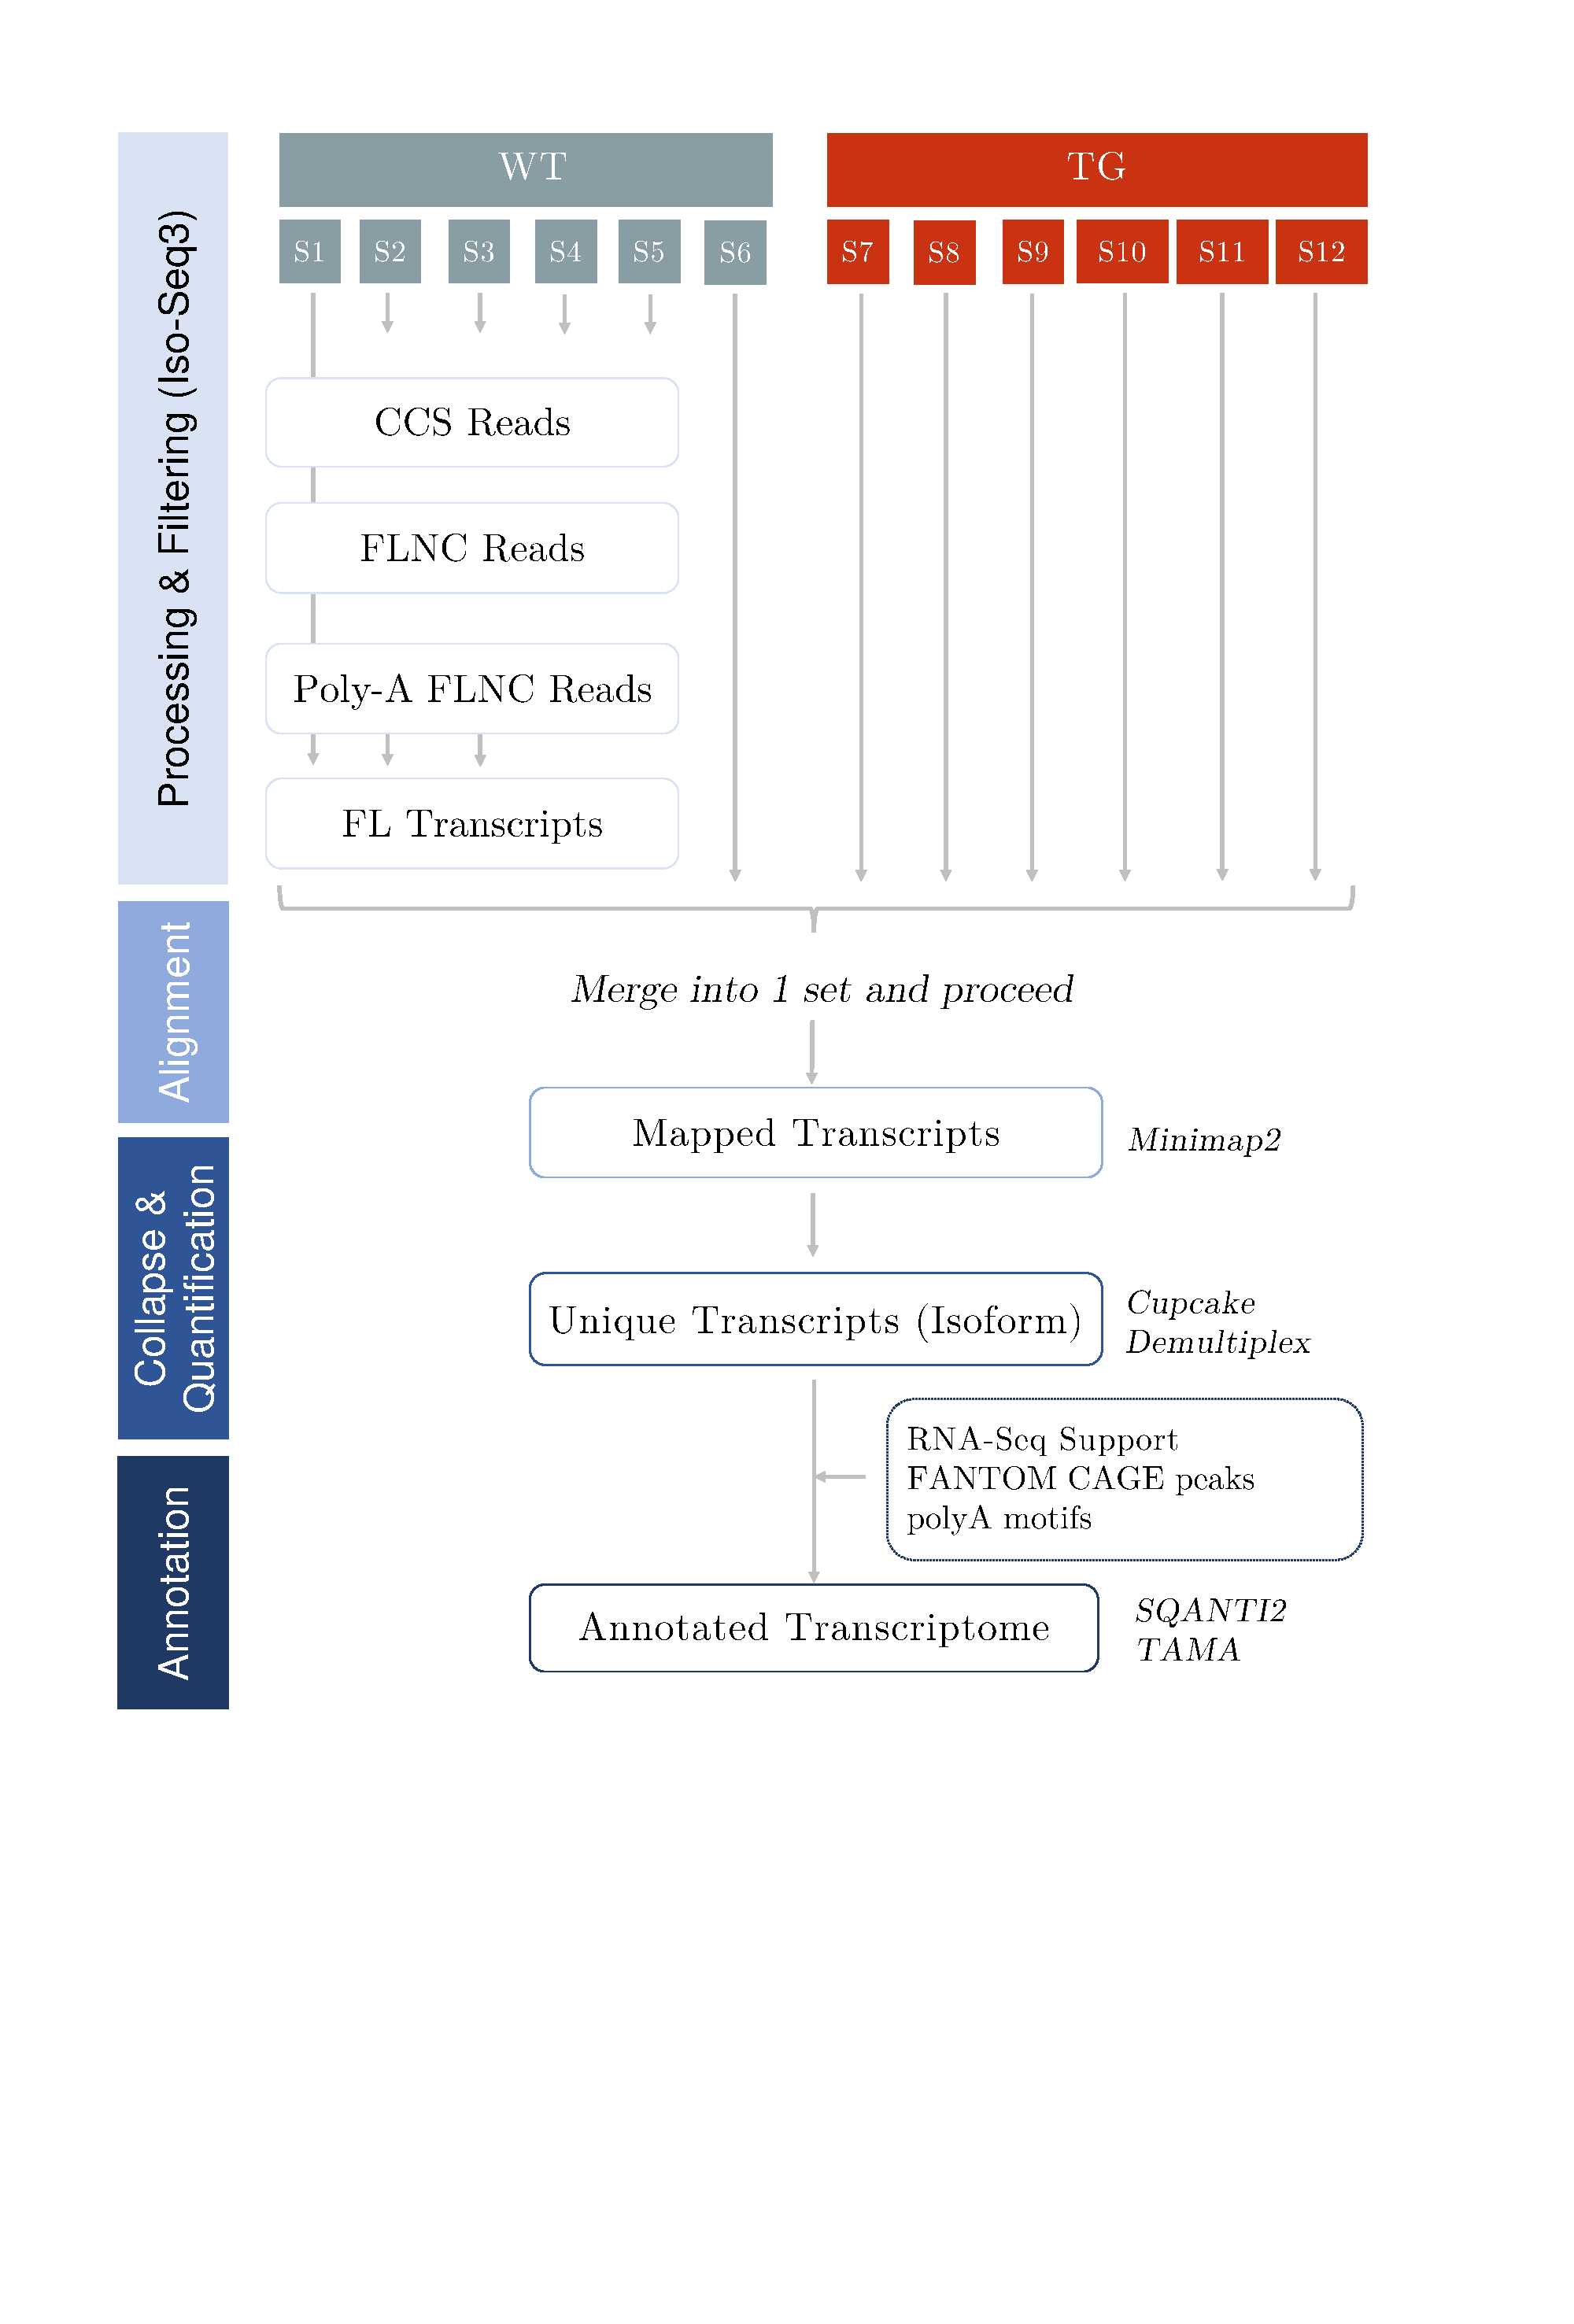
\includegraphics[page=1,trim={0 12cm 2cm 1cm},clip, scale = 0.45]{Figures/Pipeline.pdf}
	\captionsetup{width=0.95\textwidth}
	\caption[PacBio Isoseq Bioinformatics Pipeline]%
	{\textbf{PacBio Isoseq Bioinformatics Pipeline}: Pipeline is adapted from ToFU \nomenclature{ToFU}{Transcript isOforms: Full-length and Unassembled} \cite{Gordon2015}}
	\label{fig:isoseq_whole_pipeline}
\end{figure}
 
\subsection{Characterisation of Alternative Splicing Events} 
\label{sec:AS_methods}
Alternative splicing events were assessed using a range of packages and custom scripts: mutually exclusive exons (MX) and skipped exons (SE) were assessed using SUPPA with the parameter –f ioe, intron retention (IR) with SQANTI2, and alternative first exons (AF), alternative last exons (AL), alternative 5’ splice sites (A5), and alternative 3’ splice sites (A3) using custom scripts based on splice junction coordinates. 


\newpage
\section{Results}

12 mouse samples (6 WT and 6 TG) was sequenced using Iso-Seq approach on the PacBio Sequel 1 platform and analysed together for an accurate,deep characterisation of the full-length splice variants and identification of novel isoforms in the mouse transcriptome. 

\subsection{PacBio's Iso-Seq run performance and sequencing metrics}
Following library preparation and single-molecule real time sequencing (SMRT), a total of 371Gb (s.d = 4.35Gb, range = 22.5Gb - 38.74Gb) and 8,082,647 polymerase reads (s.d = 63,013 reads, range = 530,974 - 733,495 reads) were obtained (\cref{tab:isoseq_wholerun_output}). No significant difference was reported between WT and TG (n = 12 animals, two-tailed unpaired t-test, t(10) = -0.636, P = 0.539,  \cref{fig:isoseq_whole_run_output}\textbf{a}), and no significant correlation was observed between run yield and RIN across samples (n = 12 animals, Pearson's correlation, t = -0.98, df = 10, P = 0.350, \cref{fig:isoseq_whole_run_output}\textbf{b}). Yield across all the samples were within the range as would expected from SMRT Iso-Seq library.   

%Check no difference between lengths CCS read lengths i.e. equal representation of RNA molecules; to make sure that we have a fair representation of reads of the RNA transcripts --> comparison of CCS reads and representation of RNA molecules between different base pairs lengths between different sample sets --> if fair representation, then expect log-ratio of interested sample/compared sample = - (10^0 =1)

\
\begin{table}[h]
	\begin{tabularx}{1\textwidth}{cccccc}
		\toprule
		Sample & Age      & Phenotype & RIN & Total Bases (GB) & Unique Yield (GB) \\ \midrule
		K17    & 2 months & WT   & 9.2 & 29.56            & -                           \\
		K18    & 2 months & TG   & 8.8 & 31.1             & 1.21                        \\
		K23    & 8 months & WT   & 9.1 & 34.60            & 2.06                        \\
		K24    & 8 months & TG   & 9.2 & 34.61            & 2.09                        \\
		L22    & 8 months & TG   & 8.7 & 38.74            & 2.1                         \\
		M21    & 2 months & WT   & 9.2 & 30.45            & -                           \\
		O18    & 2 months & TG   & 8.9 & 22.53            & 1.56                        \\
		O23    & 8 months & WT   & 9   & 31.25            & -                           \\
		Q20    & 8 months & TG   & 8.6 & 33.16            & 2.27                        \\
		Q21    & 2 months & WT   & 9.2 & 24.52            & 2.27                        \\
		S18    & 2 months & TG   & 8.9 & 30.41            & 1.69                        \\
		S23     & 8 months & WT   & 9.1 & 30.28            & -                          \\ \bottomrule
	\end{tabularx}
	\caption[Run Yield Output from Whole Transcriptome Iso-Seq of Tg4510]%
	{Phenotypic information and Iso-seq run yield for each sample of Tg4510 sequenced using Whole Transcriptome approach}
	\label{tab:isoseq_wholerun_output}
\end{table}

\begin{figure}[h]
	\begin{center}
	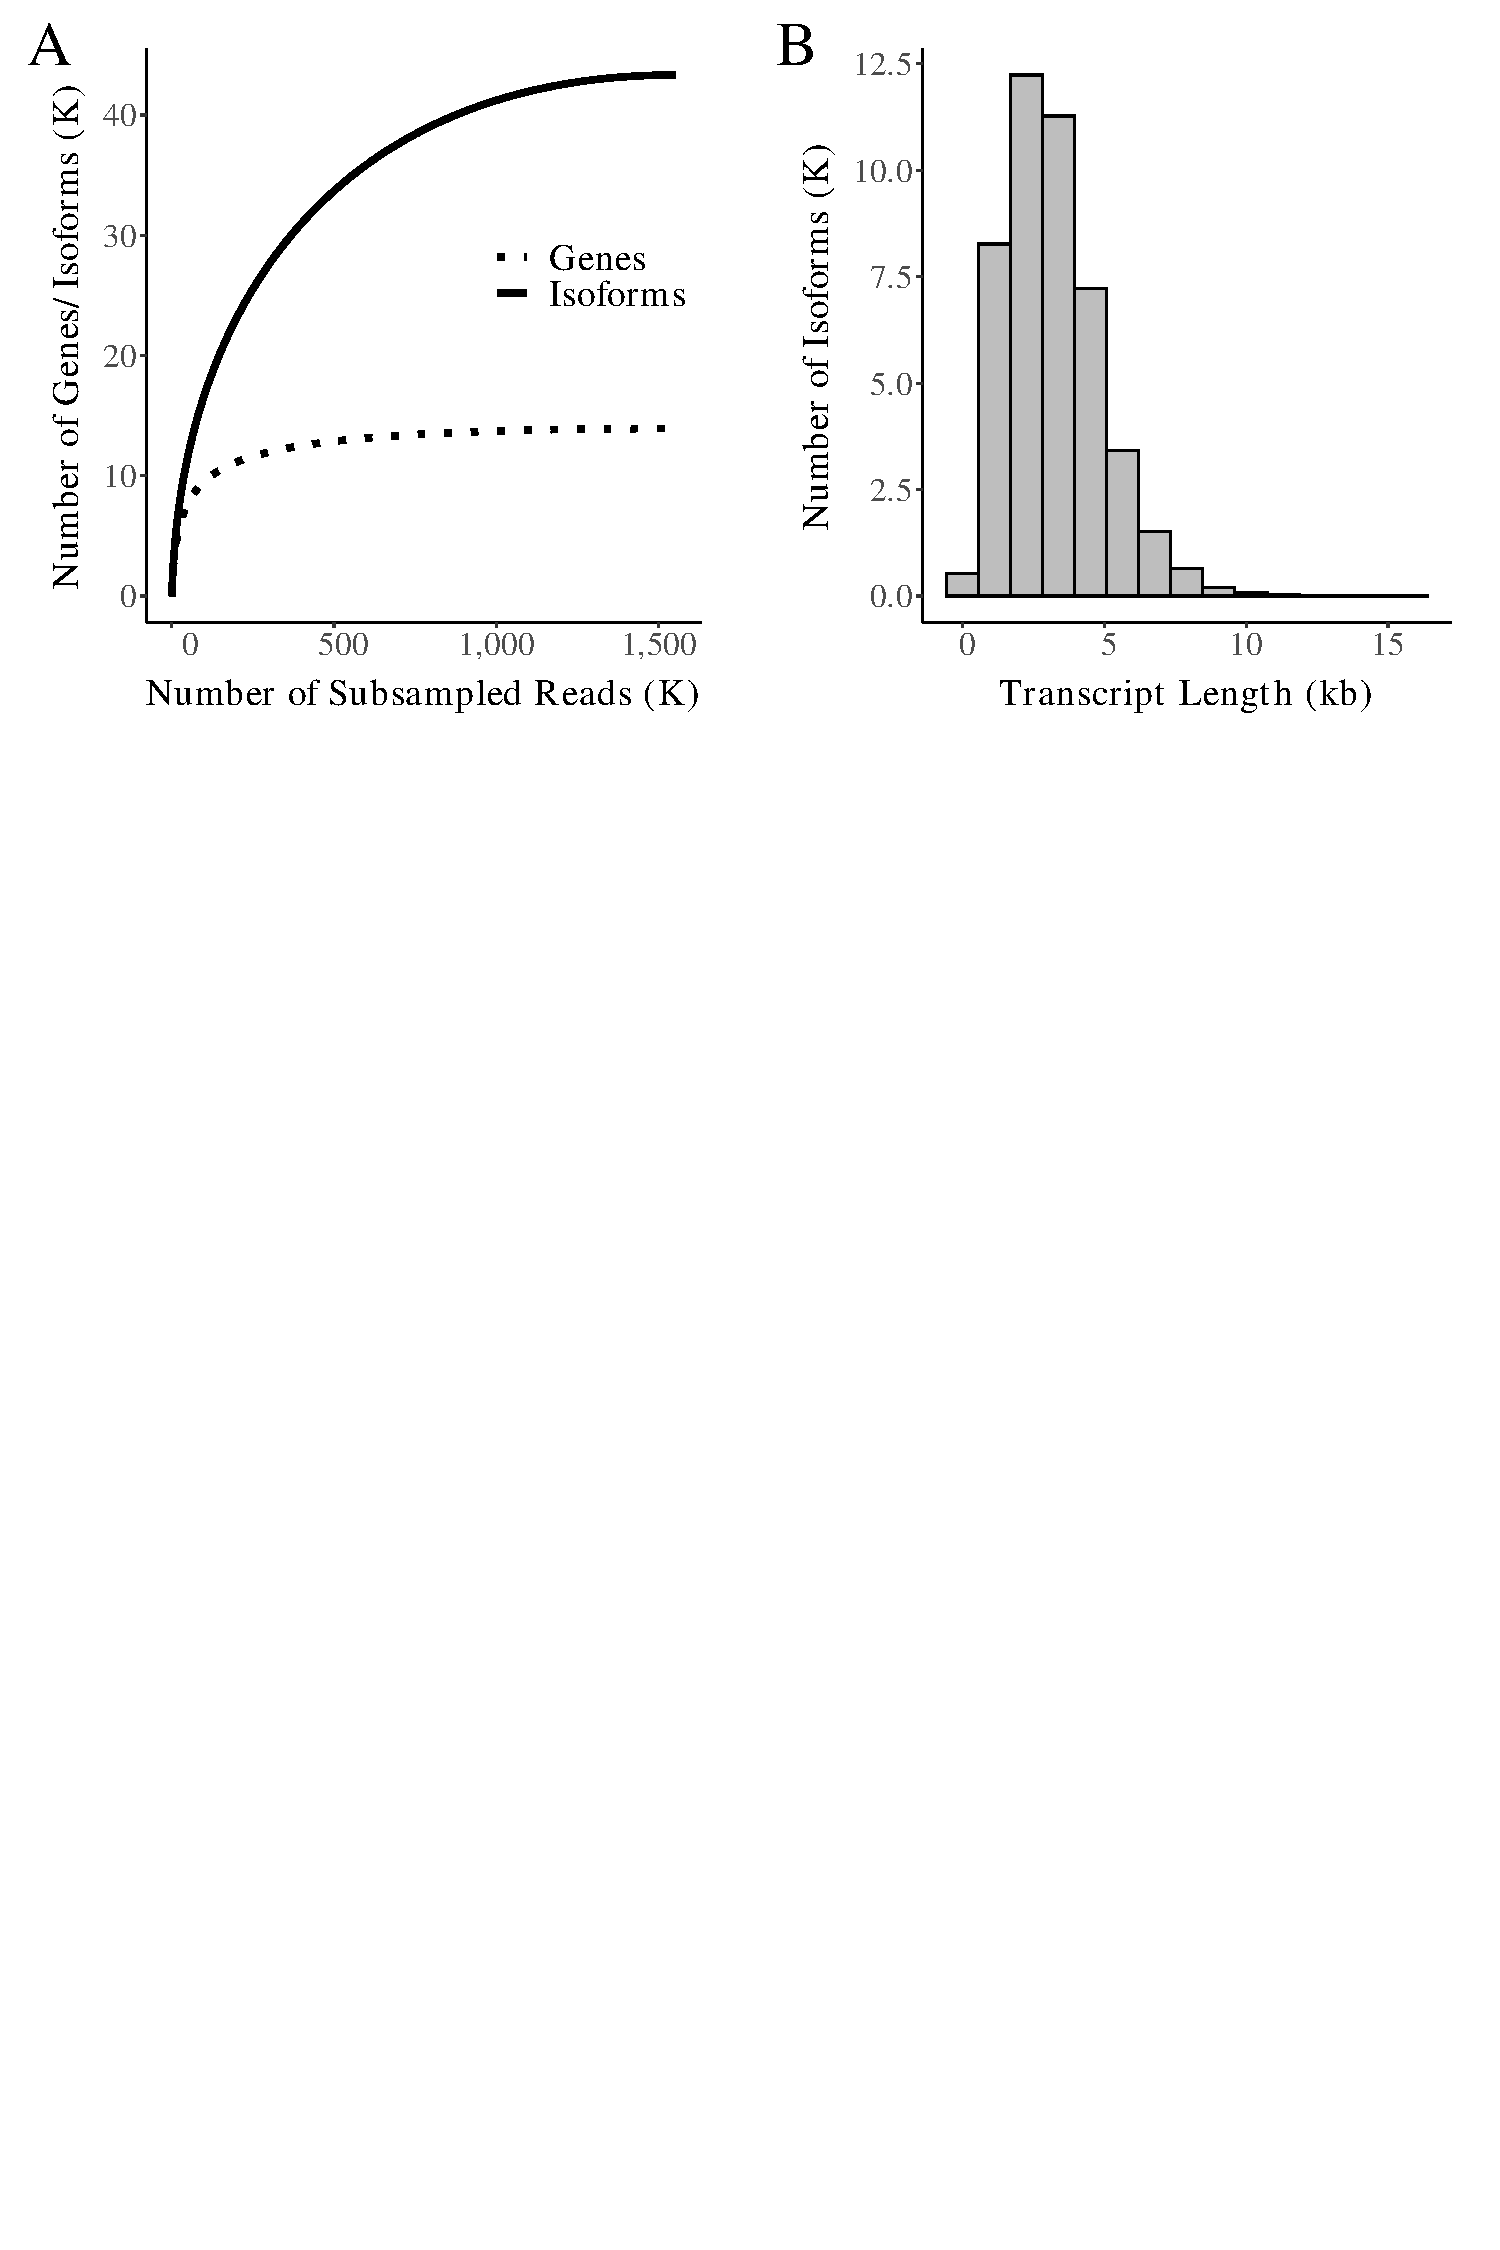
\includegraphics[page=1,trim={0 1cm 0 0},clip,scale = 0.55]{Figures/IsoSeqWholeTranscriptome.pdf}
	\end{center}
	\captionsetup{width=0.95\textwidth}
	\caption[Whole Transcriptome Iso-Seq run yields and relationship to RIN score]%
	{\textbf{Whole Transcriptome Iso-Seq runs generated \textasciitilde30Gb per sample, independent of RIN score}: Sequential Iso-Seq run generated \textbf{a)} a range of 30-35Gb per sample of the whole transcriptome, with no significant difference observed between WT and TG Tg4510 mice. Of note, two samples with $<$25Gb in WT and TG refer to earlier samples sequenced with a lower chemistry. \textbf{b)} Despite TG samples having distinctly lower RIN values than WT samples, no significant difference in yield output was observed between WT and TG.}
	\label{fig:isoseq_whole_run_output}
\end{figure}

\begin{landscape}
	\begin{table}[]
		\resizebox{1.5\textwidth}{!}{%
		\begin{tabular}{@{}cccccccccccccccccc@{}}
			\toprule
			\multirow{3}{*}{Sample} &
			\multirow{3}{*}{\begin{tabular}[c]{@{}c@{}}Polymerase\\ Reads\end{tabular}} &
			\multicolumn{6}{c}{Read   Length} &
			\multicolumn{3}{c}{Productivity} &
			\multicolumn{4}{c}{Control} &
			\multirow{3}{*}{\begin{tabular}[c]{@{}c@{}}Local\\  Base \\ Rate\end{tabular}} &
			\multicolumn{2}{c}{Template} \\ \cmidrule(lr){3-15} \cmidrule(l){17-18} 
			&
			&
			\multicolumn{2}{c|}{Polymerase} &
			\multicolumn{2}{c|}{Subread} &
			\multicolumn{2}{c|}{Insert} &
			\multicolumn{1}{c|}{\multirow{2}{*}{P0}} &
			\multicolumn{1}{c|}{\multirow{2}{*}{P1}} &
			\multicolumn{1}{c|}{\multirow{2}{*}{P2}} &
			\multicolumn{1}{c|}{\multirow{2}{*}{\begin{tabular}[c]{@{}c@{}}Total   \\ Reads\end{tabular}}} &
			\multicolumn{1}{c|}{\multirow{2}{*}{\begin{tabular}[c]{@{}c@{}}Pol RL  \\ Mean\end{tabular}}} &
			\multicolumn{2}{c|}{Concordance} &
			&
			\multicolumn{1}{c|}{\multirow{2}{*}{\begin{tabular}[c]{@{}c@{}}Adapter   \\ Dimer \\ (0-10bp)\end{tabular}}} &
			\multicolumn{1}{c|}{\multirow{2}{*}{\begin{tabular}[c]{@{}c@{}}Short\\  Insert\\  (11- 100bp)\end{tabular}}} \\ \cmidrule(lr){3-8} \cmidrule(lr){14-15}
			&
			&
			\multicolumn{1}{c|}{Mean} &
			\multicolumn{1}{c|}{N50} &
			\multicolumn{1}{c|}{Mean} &
			\multicolumn{1}{c|}{N50} &
			\multicolumn{1}{c|}{Mean} &
			\multicolumn{1}{c|}{N50} &
			\multicolumn{1}{c|}{} &
			\multicolumn{1}{c|}{} &
			\multicolumn{1}{c|}{} &
			\multicolumn{1}{c|}{} &
			\multicolumn{1}{c|}{} &
			\multicolumn{1}{c|}{Mean} &
			\multicolumn{1}{c|}{Mode} &
			&
			\multicolumn{1}{c|}{} &
			\multicolumn{1}{c|}{} \\ \midrule
			B21 &
			735598 &
			39971 &
			82100 &
			1531 &
			2125 &
			3162 &
			3896 &
			\begin{tabular}[c]{@{}c@{}}8.71\% \\ (87817)\end{tabular} &
			\begin{tabular}[c]{@{}c@{}}73.94\% \\ (745646)\end{tabular} &
			\begin{tabular}[c]{@{}c@{}}18.33\% \\ (184883)\end{tabular} &
			9940 &
			34144 &
			0.85 &
			0.89 &
			2.61 &
			0 &
			0 \\
			C20 &
			749931 &
			45670 &
			91153 &
			1426 &
			2066 &
			3204 &
			4075 &
			\begin{tabular}[c]{@{}c@{}}10.68\% \\ (107699)\end{tabular} &
			\begin{tabular}[c]{@{}c@{}}75.36\% \\ (759912)\end{tabular} &
			\begin{tabular}[c]{@{}c@{}}14.95\% \\ (150735)\end{tabular} &
			9910 &
			37019 &
			0.85 &
			0.89 &
			2.75 &
			0 &
			0 \\
			C21 &
			530395 &
			44208 &
			87750 &
			2258 &
			2794 &
			3358 &
			4250 &
			\begin{tabular}[c]{@{}c@{}}38.0\% \\ (387661)\end{tabular} &
			\begin{tabular}[c]{@{}c@{}}52.5\% \\ (535299)\end{tabular} &
			\begin{tabular}[c]{@{}c@{}}9.4\% \\ (96275)\end{tabular} &
			4880 &
			50690 &
			0.85 &
			0.85 &
			2.07 &
			0.00 &
			0.01 \\
			E18 &
			545,272 &
			41,036 &
			83,295 &
			2,467 &
			3,049 &
			3,588 &
			4,335 &
			\begin{tabular}[c]{@{}c@{}}38.88\% \\ (396026)\end{tabular} &
			\begin{tabular}[c]{@{}c@{}}53.61\% \\ (546027)\end{tabular} &
			\begin{tabular}[c]{@{}c@{}}7.58\% \\ (77181)\end{tabular} &
			722 &
			48,253 &
			0.85 &
			0.85 &
			2 &
			0 &
			0 \\
			K17 &
			673972 &
			43856 &
			90561 &
			1253 &
			2021 &
			3336 &
			4753 &
			\begin{tabular}[c]{@{}c@{}}10.55\% \\ (106,736)\end{tabular} &
			\begin{tabular}[c]{@{}c@{}}67.42\% \\ (681,794)\end{tabular} &
			\begin{tabular}[c]{@{}c@{}}22.73\% \\ (229,816)\end{tabular} &
			7036 &
			34651 &
			0.85 &
			0.89 &
			2.72 &
			0.08 &
			0.06 \\
			K18 &
			566086 &
			54892 &
			101220 &
			1256 &
			1775 &
			2863 &
			3661 &
			\begin{tabular}[c]{@{}c@{}}29.77\%\\ (299933)\end{tabular} &
			\begin{tabular}[c]{@{}c@{}}57.25\% \\ (576863)\end{tabular} &
			\begin{tabular}[c]{@{}c@{}}14.05\% \\ (141550)\end{tabular} &
			10707 &
			44640 &
			0.87 &
			0.89 &
			3.05 &
			0 &
			0 \\
			K23 &
			698178 &
			49563 &
			98801 &
			1697 &
			2670 &
			3779 &
			4779 &
			\begin{tabular}[c]{@{}c@{}}16.1\% \\ (164308)\end{tabular} &
			\begin{tabular}[c]{@{}c@{}}69.2\%  \\ (704197)\end{tabular} &
			\begin{tabular}[c]{@{}c@{}}14.7\%   \\ (149841)\end{tabular} &
			5951 &
			40498 &
			0.85 &
			0.89 &
			2.78 &
			0 &
			0 \\
			K24 &
			711015 &
			48675 &
			97024 &
			1714 &
			2487 &
			3834 &
			5018 &
			\begin{tabular}[c]{@{}c@{}}14.22\% \\ (144813)\end{tabular} &
			\begin{tabular}[c]{@{}c@{}}70.49\%\\  (717880)\end{tabular} &
			\begin{tabular}[c]{@{}c@{}}15.28\% \\ (155653)\end{tabular} &
			6762 &
			38363 &
			0.85 &
			0.87 &
			2.671 &
			0.01 &
			0.01 \\
			L22 &
			675283 &
			57370 &
			112630 &
			1869 &
			2867 &
			3903 &
			4793 &
			\begin{tabular}[c]{@{}c@{}}17.41\%\\ (175439 )\end{tabular} &
			\begin{tabular}[c]{@{}c@{}}68.08\%\\ (686007)\end{tabular} &
			\begin{tabular}[c]{@{}c@{}}15.58\% \\ (156900)\end{tabular} &
			10647 &
			44215 &
			0.86 &
			0.89 &
			2.96 &
			0.01 &
			0 \\
			M21 &
			660841 &
			46082 &
			91628 &
			2234 &
			2754 &
			3952 &
			4733 &
			\begin{tabular}[c]{@{}c@{}}16.6\%\\ (168567)\end{tabular} &
			\begin{tabular}[c]{@{}c@{}}65.9\%  \\ (671224)\end{tabular} &
			\begin{tabular}[c]{@{}c@{}}17.5\% \\  (178555)\end{tabular} &
			10301 &
			38690 &
			0.85 &
			0.87 &
			2.79 &
			0.01 &
			0.01 \\
			O18 &
			530974 &
			42423 &
			85331 &
			2609 &
			3146 &
			3443 &
			4082 &
			\begin{tabular}[c]{@{}c@{}}41.8\% \\  (426378\end{tabular} &
			\begin{tabular}[c]{@{}c@{}}52.6\%\\  (536435)\end{tabular} &
			\begin{tabular}[c]{@{}c@{}}5.5\% \\ (56422)\end{tabular} &
			5415 &
			49778 &
			0.86 &
			0.85 &
			2.05 &
			0 &
			0 \\
			O23 &
			730733 &
			42771 &
			89372 &
			1490 &
			2347 &
			3608 &
			4878 &
			\begin{tabular}[c]{@{}c@{}}9.37\% \\ (94536)\end{tabular} &
			\begin{tabular}[c]{@{}c@{}}73.33\% \\ (740184)\end{tabular} &
			\begin{tabular}[c]{@{}c@{}}18.19\% \\ (183626)\end{tabular} &
			8908 &
			34993 &
			0.85 &
			0.89 &
			2.56 &
			0.06 &
			0.04 \\
			Q20 &
			715206 &
			46360 &
			92519 &
			1,999 &
			2,926 &
			3,978 &
			4,954 &
			\begin{tabular}[c]{@{}c@{}}11.51\%\\  (117223)\end{tabular} &
			\begin{tabular}[c]{@{}c@{}}70.91\% \\ (722135)\end{tabular} &
			\begin{tabular}[c]{@{}c@{}}17.58\%\\  (178988)\end{tabular} &
			6855 &
			37990 &
			0.85 &
			0.87 &
			2.6 &
			0.01 &
			0.01 \\
			Q21 &
			733495 &
			33429 &
			70750 &
			2563 &
			3286 &
			3710 &
			4750 &
			\begin{tabular}[c]{@{}c@{}}15.9\% \\ (161679)\end{tabular} &
			\begin{tabular}[c]{@{}c@{}}72.1\%\\  (735250)\end{tabular} &
			\begin{tabular}[c]{@{}c@{}}12.0\% \\ (122305)\end{tabular} &
			1668 &
			44201 &
			0.85 &
			0.85 &
			1.99 &
			0.00 &
			0.01 \\
			S18 &
			682529 &
			44549 &
			90041 &
			1435 &
			2041 &
			3282 &
			4400 &
			\begin{tabular}[c]{@{}c@{}}11.98\%\\  (121,055)\end{tabular} &
			\begin{tabular}[c]{@{}c@{}}68.45\% \\ (691651)\end{tabular} &
			\begin{tabular}[c]{@{}c@{}}20.35\%\\  (205,640)\end{tabular} &
			7881 &
			36541 &
			0.86 &
			0.89 &
			2.85 &
			0.11 &
			0.07 \\
			S23 &
			704335 &
			42991 &
			89160 &
			1346 &
			2020 &
			3272 &
			4383 &
			\begin{tabular}[c]{@{}c@{}}7.02\%\\  (71074)\end{tabular} &
			\begin{tabular}[c]{@{}c@{}}70.18\% \\ (710471)\end{tabular} &
			\begin{tabular}[c]{@{}c@{}}23.39\% \\ (236801)\end{tabular} &
			6019 &
			35167 &
			0.85 &
			0.89 &
			2.57 &
			0.01 &
			0.01 \\ \bottomrule
		\end{tabular}%
	}
	\end{table}
\end{landscape}

With the application of long-reads bioinformatics pipeline (as detailed in Section X), the raw reads were processed and clustered to unique consensus transcripts, which were then mapped and annotated as isoforms - low-quality, lowly-supported, unmapped and degraded reads were sequentially filtered at each stage. Across all 12 samples, a total of 5.66M CCS reads (mean = 471K,s.d = 46.8K, range =  353K - 512K) and 4.55 FLNC reads were successfully generated (mean = 379K, s.d = 47.0K, range = 270K - 412K) after multiple processing (\cref{fig:isoseq_whole_processing}\textbf{a}). Clustering of these reads yielded a total of 273K high-quality full-length transcripts (97\% of all FL transcripts, mean = 32.7K, s.d = 1.25K, range = 30.3K - 34.4K) (\cref{fig:isoseq_whole_processing}\textbf{b}), and were mapped to 278K and 352 loci of the mouse reference (5K had multi-mapping) and ERCC annotations respectively. After filtering for 85\% alignment identity and 95\% length (\cref{fig:isoseq_whole_processing}\textbf{c}), 266K transcripts were retained. 

Showcasing the sensitivity of the sequencing platform and approach, only 62\% (n = 57) of ERCCs were detected, those of which were more highly expressed and with a threshold concentration of XX (\cref{fig:isoseq_whole_ercc}\textbf{a}). However of those ERCCs detected, the number of FL reads detected was highly correlated to the known amount used (corr = 0.98, P = 1.42 x 10\textsuperscript{-41} \cref{fig:isoseq_whole_ercc}\textbf{b}), highlighting the power of Iso-Seq to quantify highly-expressed transcripts. 

\begin{figure}[htp]
	\begin{center}
		\includegraphics[page=11,trim={0 1cm 0 0},clip,scale = 0.55]{Figures/IsoSeqWholeTranscriptome.pdf}
	\end{center}
	\captionsetup{width=0.95\textwidth}
	\caption[Whole Transcriptome Iso-Seq run yields and relationship to RIN score]%
	{\textbf{Whole Transcriptome Iso-Seq runs generated \textasciitilde30Gb per sample, independent of RIN score}: Sequential Iso-Seq run generated \textbf{a)} a range of 30-35Gb per sample of the whole transcriptome, with no significant difference observed between WT and TG Tg4510 mice. Of note, two samples with $<$25Gb in WT and TG refer to earlier samples sequenced with a lower chemistry. \textbf{b)} Despite TG samples having distinctly lower RIN values than WT samples, no significant difference in yield output was observed between WT and TG.}
	\label{fig:isoseq_whole_lengths}
\end{figure}

\begin{figure}[htp]
	\begin{center}
		\includegraphics[page=2,scale = 0.55]{Figures/IsoSeqWholeTranscriptome.pdf}
	\end{center}
	\captionsetup{width=0.95\textwidth}
	\caption[Sequential processing and alignment of reads from Whole Transcriptome Iso-Seq run]%
	{\textbf{Sequential processing of Iso-Seq Reads generated around 32K transcripts per sample with good alignment to reference genome}: \textbf{a)} Processing of Iso-Seq reads generated a similar number of reads across all sample throughout Iso-Seq3 bioinformatis pipeline, with the exception of 2 earlier samples. \textbf{b)} Despite this, all the samples had similar number of FL transcripts with no signficant difference observed between WT and TG. \textbf{c)}The majority of transcipts aligned to mouse reference genome (mm10) with >85\% alignment identity and $>$95\% length}
	\label{fig:isoseq_whole_processing}
\end{figure}

\begin{figure}[htp]
	\begin{center}
		\includegraphics[page=6,trim={0 25cm 0 0},clip,scale = 0.55]{Figures/IsoSeqWholeTranscriptome.pdf}
	\end{center}
	\captionsetup{width=0.95\textwidth}
	\caption[Detection of ERCC standards in Whole Transcriptome Iso-Seq]%
	{\textbf{Over 60\% of ERCCs were detected with highly accurate quantification} \textbf{a} Highly-concentrated ERCCs were detected as single molecules, as expected, and \textbf{b} the number of full-length reads associated for each detected ERCC was highly correlated to known amount. FL - Full Length}
	\label{fig:isoseq_whole_ercc}
\end{figure}


\newpage
\subsection{Nanopore Sequencing run performance and sequencing metrics}
As a technological comparison, two of the samples sequenced on the PacBio Sequel were also sequenced on the ONT MinION. In contrast to the Iso-Seq, the run performance and yield was significantly poorer and lower with greater variability observed between the two samples (K18: 10.1Gb from nanopore vs 31.1Gb from Iso-Seq, M21: 3.68Gb from nanopore vs 30.45Gb from Iso-Seq, \cref{tab:ont_wholerun_output}). The significantly low performance of M21 was due to saturation and permanent blocking of pores (\cref{fig:ont_seq_channel}\textbf{b}) with more rapid decline of sequencing activity than is expected (\cref{fig:ont_time_performance}\textbf{b}). No difference in the sequencing speed was observed across the course of the run (\cref{fig:ont_speedvstime}), however, suggesting that the sequencing chemistry and flow cell was of good quality. The low performance output of the second sample is therefore likely due to introduction of air bubbles and contamination during library preparation.

After removing low-quality basecalled reads (QV < 7), a total of 6M reads were acquired (K18: 4.49M reads, 66\% of total reads, M21: 1.68M reads, 79.2\%, \cref{tab:ont_passedreads_output}). Interestingly, despite the marked lower run performance of the second sample, the read quality was slightly higher (K18: mean QV = 9.5, M21: mean QV = 10.2) whereby the first sample had a large portion of very low-quality reads (QV < 2, \cref{fig:ont_lengthquality}\textbf{a}). Nevertheless, both samples had a very similar read length distribution profile (\cref{fig:ont_lengthquality}\textbf{c,d}), with a mean length around 1.8Kb. However in contrast to Iso-Seq, the distribution is skewed to the left with enrichment of smaller molecules (1kb) - a likely reflection of the library size with no size enrichment during library preparation rather than a length bias of the technology. 

Despite the relatively low run performance, more reads were acquired per flow cell per sample than per SMRT cell in Iso-Seq (mean number of basecalled reads from nanopore across 2 samples: 4.43M, mean number of polymerase reads from Iso-Seq across 12 samples: 0.67M). This is because while Iso-Seq was able to generate very long polymerase reads (mean length across 12 samples = 46kb), contributing to the run yield in gigabases, the number of reads generated per run was limited to 1M (number of SMRT cells). Conversely, there was no upper limit in the number of reads that can be generated with nanopore sequencing provided the pores remained active. A greater proportion of ERCCs (68 ERCCs, 73.9\%) was therefore observed in one nanopore run compared to 12 Iso-Seq runs (57 ERCCs, 62\%), and for those ERCCs detected, the number of FL reads detected was also highly correlated to the known amount used (corr = 0.98, P = 9.73 x 10\textsuperscript{-51}). 


\vspace{1cm}
\begin{table}[ht]
	\centering
	\begin{tabularx}{1\textwidth}{@{}ccccc@{}}
		\toprule
		\multirow{2}{*}{Sample} & \multicolumn{2}{c}{All Reads}      & \multirow{2}{*}{Active channels} & \multirow{2}{*}{Run Duration} \\ \cmidrule(lr){2-3}
		& Total Bases (Gb) & Number of Reads &                                  &                               \\ \midrule
		K18                     & 10.1             & 6,752,951       & 479                              & 48hours                       \\
		M21                     & 3.68             & 2,122,012       & 425                              & 48hours                       \\ \bottomrule
	\end{tabularx}
	\captionsetup{justification=raggedright,width=0.95\textwidth}
\caption[Run Yield Output from Whole Transcriptome Nanopore Sequencing of Tg4510]%
{\textbf{Poorer run performance and lower yield output observed from Nanopore Sequencing of Whole Transcriptome}. Two samples, sequenced on PacBio Sequel using Iso-Seq approach, were also sequenced on ONT MinION on two separate flow cells over 48hours. The number of total reads basecalled was less than a third of the reads generated on the same samples from the Iso-Seq approach (\cref{tab:isoseq_wholerun_output})}
\label{tab:ont_wholerun_output}
\end{table}

\vspace{2cm}
\begin{table}[ht]
	\centering
	\begin{tabularx}{1\textwidth}{@{}ccccccccc@{}}
		\toprule
		\multirow{2}{*}{Sample} & \multirow{2}{*}{\begin{tabular}[c]{@{}c@{}}Total Bases\\ (Gb)\end{tabular}} & \multirow{2}{*}{\begin{tabular}[c]{@{}c@{}}Number of\\  Reads\end{tabular}} & \multicolumn{4}{c}{Read Length (bp)} & \multicolumn{2}{c}{Read Quality} \\ \cmidrule(l){4-9} 
		&                                                                             &                                                                             & Median  & Mean & N50  & Longest Read & Median           & Mean          \\ \midrule
		K18                     & 8.21                                                                        & \begin{tabular}[c]{@{}c@{}}4,468,629 \\ (66.2\%)\end{tabular}               & 1400    & 1838 & 2521 & 48877        & 9.6              & 9.5           \\
		M21                     & 3.1                                                                         & \begin{tabular}[c]{@{}c@{}}1,679,931\\  (79.2\%)\end{tabular}               & 1410    & 1845 & 2644 & 82984        & 10.3             & 10.2          \\ \bottomrule
	\end{tabularx}
	\captionsetup{justification=raggedright,width=0.95\textwidth}
	\caption[ONT Sequencing metrics for pass basecalled reads]%
	{\textbf{Sequencing metrics of filtered high-quality reads}. Basecalled reads were filtered on quality score with a QV threshold of 7. N50 refers to the sequence length at which 50\% of reads are sized at or over. Gb - Gigabases}
	\label{tab:ont_passedreads_output}
\end{table}

\begin{figure}[htp]
	\begin{center}
		\includegraphics[page=1,scale = 0.45]{Figures/ONTWholeTranscriptome.pdf}
	\end{center}
	\captionsetup{width=0.95\textwidth}
	\caption[ONT Sequence Channel Activity from Whole Transcriptome Sequencing ]%
	{\textbf{Sequencing channel activity plot from nanopore sequencing}. Heatmap representation of channel productivity spatially for \textbf{a)} Sample K18 (10.1Gb) and \textbf{b)} Sample M21 (3.68Gb) as DNA is translocated through the pore and signal is collected. A stark contrast of activity can be seen between the two samples, with a significant number of inactive channels (white box) in Sample M21 - of the channels that are active, fewer DNA molecules are translocated and read.  Of note, the activity shows the number of sequences generated per channel not per pore, given that each channel corresponds to four different pores.}
	\label{fig:ont_seq_channel}
\end{figure}

\begin{figure}[htp]
	\begin{center}
		\includegraphics[page=2,,trim={0 0cm 0cm 10cm},clip, scale = 0.45]{Figures/ONTWholeTranscriptome.pdf}
	\end{center}
	\captionsetup{width=0.95\textwidth}
	\caption[ONT run performance over time from Whole Transcriptome Sequencing ]%
	{\textbf{Temporal run performance from nanopore sequencing}. Shown is the \textbf{a)} number of basses generated per hour over the course of the sequencing run from Sample K18 and from \textbf{b)} Sample M21, and \textbf{c)} cumulative reads generated from Sample K18 and from \textbf{d)} Sample M21. The reads are classified as "pass" (dark blue) if QV > 7 and "fail" (light blue) if QV < 7. The rapid decline of pore activity of Sample M21 is evident from Figure b) in contrast to Figure a), with 90\% of the sequencing data acquired within the first 10hours of the run (Figure d). T50 and T90 refers to the time point at which 50\% and 90\% of total basecalled reads where acquired respectively. Gb - Gigabases}
	\label{fig:ont_time_performance}
\end{figure}

\begin{figure}[htp]
	\begin{center}
		\includegraphics[page=4,trim={1cm 0cm 0cm 20cm},clip, scale = 0.45]{Figures/ONTWholeTranscriptome.pdf}
	\end{center}
	\captionsetup{width=0.95\textwidth}
	\caption[ONT translocation speed against time from Whole Transcriptome Sequencing]%
	{\textbf{DNA translocation speed against time}. A boxplot of the translocation speed (sequencing rate) for Sample M21 over the course of the 48-hour run. }
	\label{fig:ont_speedvstime}
\end{figure}

\begin{figure}[htp]
	\begin{center}
		\includegraphics[page=3,trim={0 0cm 0cm 10cm},clip, scale = 0.45]{Figures/ONTWholeTranscriptome.pdf}
	\end{center}
	\captionsetup{width=0.95\textwidth}
	\caption[ONT read length and quality from Whole Transcriptome Sequencing ]%
	{\textbf{Length and quality distribution of ONT basecalled reads}. Shown are histograms of the number of sequenced reads against \textbf{a)} mean read quality score of Sample K18, \textbf{b)} mean read quality score of Sample M21, and against \textbf{c)} length of Sample K18 and of \textbf{d)} Sample M21. The distribution has been shaded for reads that have passed or failed the quality filter (Q-score threshold of 7). N50 refers to the sequence length at which 50\% of reads are sized at or over. }
	\label{fig:ont_lengthquality}
\end{figure}

\begin{figure}[htp]
	\begin{center}
		\includegraphics[page=4,trim={0 16cm 0cm 0},clip, scale = 0.45]{Figures/Pipeline.pdf}
	\end{center}
	\captionsetup{width=0.95\textwidth}
	\caption[ONT read quality against read length from Whole Transcriptome Sequencing ]%
	{\textbf{Distribution of quality scores against read lengths for all ONT basecalled reads}. Shown are 2D density plots for \textbf{a)} Sample K18 and \textbf{b)} Sample M21 of mean sequence quality (Phred quality score) against read length (log10). Figures are generated from PycoQC \cite{Leger2019}.}
	\label{fig:ont_lengthvsquality}
\end{figure}

\clearpage
\subsection{Transcriptome annotation}
After further collapsing and filtering of transcripts using the Iso-Seq data, a total of 46,626 unique and intact isoforms were identified (mean = 27.5K, s.d = 2.32K, range = 24.2K - 31.2K) and annotated to 14,482 (98.6\%) known and 202 (1.38\%) novel genes. Gene expression patterns from Iso-Seq reflected expected transcriptional profiles for the brain regions profiled. Using the Mouse Gene Atlas database, the 500 most abundantly-expressed genes were most significantly enriched for ‘cerebral cortex’ (odds ratio = 6.07, adjusted P = 6.8 x 10\textsuperscript{-17}). Rarefaction curves confirmed that the dataset approached saturation, indicating that our coverage of isoform diversity was representative of the true population of transcripts (\cref{fig:isoseq_whole_rarefaction}\textbf{a}). Supporting the validity of these isoforms, the majority (n = 35,262, 75\% of isoforms) were enriched near an annotated CAGE peaks (located within 50bp), and the vast majority of unique splice junctions (n = 138,032, 97.8\% of junctions) were supported by RNA-Seq.

\begin{figure}[htp]
	\begin{center}
		\includegraphics[page=3,scale = 0.55]{Figures/IsoSeqWholeTranscriptome.pdf}
	\end{center}
	\captionsetup{width=0.95\textwidth}
	\caption[Rarefaction Curves of Whole Transcriptome Iso-Seq Runs]%
	{\textbf{Rarefaction curve of Iso-Seq merged dataset indicated saturation and good coverage of genes and isoforms}:}
	\label{fig:isoseq_whole_rarefaction}
\end{figure}

\newpage
\subsection{Isoform diversity}
Compared with the mouse reference genome, there was a wider range in the number of isoforms identified per gene (1 – 86), with each gene associated with a median of 2 isoforms. Only 10\% (n = 4,641) of isoforms were detected across all the samples (\cref{fig:isoseq_whole_lowlyexp}\textbf{a}), with about half (47.8\%) detected in 2 - 3 samples with very low transcript expression (\cref{fig:isoseq_whole_lowlyexp}\textbf{b}).

Gene ontology (GO) analysis showed that the most enriched molecular function amongst the 100 most transcriptionally diverse genes in mouse cortex was ‘tubulin binding’ (odds ratio = 7.90, adjusted P =  6.70 x 10\textsuperscript{-4}), driven by the overexpression of MAPT in TG mice.
%an interesting observation given the role that RNA-binding proteins (RBPs) themselves play in regulating tissue-specific patterns of alternative splicing. 
%Any differences between samples not due to absence or presence of isoform but isoform proportion/ not deep enough?   
   
A significant proportion of isoforms (20,621, 45\%) were sized 2 - 4kb in length (median length = 2.96kb, mean length = 3.18kb, s.d = 1.68kb, range = 0.083 - 15.9kb) (\cref{fig:isoseq_whole_isoform_length_corr}\textbf{a}), corresponding to the mean length of mRNA mouse reference genome, with a wide range in the number of exons (1 - 89) observed per isoform (mean number of exons = 10.8). The number of isoforms per gene was correlated with gene length (corr = 0.25, P = 1.33 x 10 \textsuperscript{-197}, \cref{fig:isoseq_whole_isoform_length_corr}{c}), and exon number (corr = 0.24, P = 7.97 x 10 \textsuperscript{-155}, \cref{fig:isoseq_whole_isoform_length_corr}{d}). 

\begin{figure}[htp]
	\begin{center}
		\includegraphics[page=4,trim={0 25cm 0 0},clip,scale = 0.55]{Figures/IsoSeqWholeTranscriptome.pdf}
	\end{center}
	\captionsetup{width=0.95\textwidth}
	\caption[Isoform diversity across Tg4510 samples and coverage of ERCC transcripts]%
	{\textbf{Highly-expressed isoforms are more likely to be sequenced across sampples and accurately quantified}: Shown is \textbf{a)} the distribution of isoforms detected in the number of mouse samples, with a third detected in any two of the total 12 samples. However, \textbf{b)} quantification of these isoforms had very low expression (1-2 FL read), whereas those that were commonly detected across all 12 samples were very highly expressed. FL - Full Length}
	\label{fig:isoseq_whole_lowlyexp}
\end{figure}

\begin{figure}[htp]
	\begin{center}
		\includegraphics[page=5,trim={0 12cm 0 0},clip,scale = 0.55]{Figures/IsoSeqWholeTranscriptome.pdf}
	\end{center}
	\captionsetup{width=0.95\textwidth}
	\caption[Correlation of isoform diversity with transcript length and number of exons]%
	{\textbf{Longer genes with more exons were associated with more isoforms}: \textbf{a} The majority of isoforms have a length between 1 - 5kb. \textbf{b)} The number of exons was correlated with the transcript length, and the \textbf{c)} the number of isoforms was correlated with the length and \textbf{d)} and the number of exons per gene. Gene length and exon number is represented by the longest transcript. kb - kilobases}
	\label{fig:isoseq_whole_isoform_length_corr}
\end{figure}


\newpage
\subsection{Iso-Seq vs RNA-Seq} 
To compare the power of Iso-Seq versus RNA-Seq to detect full-length transcripts, a reference-guided transcriptome assembly using only Illumina's RNA-Seq reads of the same samples was generated with Stringtie. Using SQANTI to characterise isoforms similarly to the Iso-Seq analysis, RNA-Seq defined transcriptome revealed significantly more isoforms (156,253 isoforms vs 46,626 isoforms from Iso-Seq defined transcriptome, \cref{fig:isoseq_whole_rnaseqvsisoseq}\textbf{a}). However, upon further examination and comparison using gffcompare, majority of these isoforms were found to be incomplete fragments of isoforms identified in Iso-Seq, with significantly shorter isoform length (2.31kb vs 3.18kb of mean length of RNA-Seq and Iso-Seq defined isoforms respectively, two-tailed unpaired t-test, t(203070) = 71.9, P < 2.2 x 10\textsuperscript{-16}, \cref{fig:isoseq_whole_rnaseqvsisoseq}\textbf{c}), fewer exons (7.30 vs 10.8 of mean number of exons of RNA-Seq and Iso-Seq defined isoforms respectively, two-tailed unpaired t-test, t(203070) = 76.7, P < 2.2 x 10\textsuperscript{-16}, \cref{fig:isoseq_whole_rnaseqvsisoseq}\textbf{d}) and less supported by CAGE peaks (34.0\% vs 71.9\% of RNA-Seq and Iso-Seq defined isoforms within 50bp CAGE peak respectively, Fisher's Test: P < 2.2 x 10\textsuperscript{-16}, odds ratio = 4.97, \cref{fig:isoseq_whole_rnaseqvsisoseq}\textbf{e}). Considering only isoforms that had a complete exact match as defined by gffcompare, more than 50\% of isoforms detected from Iso-Seq dataset could not be readily recapitulated (\cref{fig:isoseq_whole_rnaseqvsisoseq}\textbf{a}), the majority of which were novel isoforms and genes (\cref{fig:isoseq_whole_rnaseqvsisoseq}f).      

The isoform expression (TPM) was then compared using the following methods: 
\begin{enumerate}
	\item Iso-Seq data alone using FL read count 
	\item RNA-Seq data aligned to Iso-Seq defined transcriptome using Kallisto\cite{Bray2016}
	\item RNA-Seq data aligned to RNA-Seq defined transcriptome using Kallisto\cite{Bray2016}. RNA-Seq transcriptome was generated using Stringtie. 	
\end{enumerate}

Focusing only on the subset of isoforms that were commonly identified in both RNA-Seq and Iso-Seq defined transcriptomes (n = 23,761), the isoform expression using RNA-Seq data mapped to Iso-Seq (method 2) and RNA-Seq transcriptome (method 3) was highly correlated (Pearson's correlation = 0.77, P < 2.2 x 10\textsuperscript{-16}). Conversely, the isoform expression derived from Iso-Seq data alone (method 1) was weekly correlated to the RNA-Seq derived isoform expression (method 3, Pearson's correlation = 0.45, P < 2.2 x 10\textsuperscript{-16}). This highlights the power of Iso-Seq defined transcriptome to accurately identify and annotate isoforms as a scaffold, but is limited for quantitative analysis due to sequencing depth.

\begin{figure}[htp]
	\begin{center}
		\includegraphics[page=13,scale = 0.55]{Figures/IsoSeqWholeTranscriptome.pdf}
	\end{center}
	\captionsetup{width=0.95\textwidth}
	\caption[RNA-Seq defined transcriptome]%
	{\textbf{Iso-Seq identified more isoforms per gene, that were longer with more exons, and with a greater proportion of isoforms with CAGE peak}: A reference-guided transcriptome using only RNA-Seq data (RNA-Seq defined transcriptome) was generated. \textbf{a)} RNA-Seq defined transcriptome identified more isoforms, as expected given the significantly higher sequencing depth. However, \textbf{b)} the isoform diversity was smaller than that from Iso-Seq defined transcriptome with the majority of genes associated with only one isoform. \textbf{c)} Isoforms identified from the RNA-Seq defined transcriptome were also more likely to be shorter and \textbf{d} contain fewer exons. \textbf{e)} Highlighting the power of Iso-Seq to identify true full-length isoforms in comparison to RNA-Seq, a significantly larger proportion of isoforms from Iso-Seq data were found within 50bp of a CAGE peak. \textbf{f} Approximately half of the isoforms identified using Iso-Seq were novel (NIC, NNC), which were not recapitulated using RNA-Seq. FSM - Full Splice Match, ISM - Incomplete Splice Match, NIC - Novel In Catalogue, NNC - Novel Not in Catalogue.}   
	\label{fig:isoseq_whole_rnaseqvsisoseq}
\end{figure}


\subsection{Novel isoforms}
\label{sec:whole_novelIso}
Interestingly, the transcriptome was made up of 50\% of isoforms that were known (23,350) and 50\% that were novel (23,096) and were not present in existing annotation databases (\cref{tab:sqanti_output_whole}). Benchmarking the accuracy and reliability of novel isoforms against known isoforms, no difference in the number supported within 50bp CAGE was observed (novel isoforms within CAGE: 17,252, 75.4\%; known isoforms with CAGE: 17,842, 75.8\%, Fisher's Test: P = 0.31, odds ratio = 0.978). Less RNA-Seq support was observed for novel isoforms compared to known isoforms (mean RNA-Seq expression for known isoforms = 8.95TPM, mean RNA-Seq expression for novel isoforms = 1.99TPM; two-tailed unpaired t-test: t(46401) = 14.8, P = 1.37 x 10\textsuperscript{-49}); however, this is likely to reflect RNA-Seq's lack of power to detect novel isoforms rather than the validity of these isoforms. 

\begin{table}[]
	\begin{tabularx}{1\textwidth}{lcl}
	\toprule
	Description              & \multicolumn{1}{l}{Number} & Isoform Definition               \\ \midrule
	Number of Genes    & 14684                      &                                  \\
	Number of Isoforms & 46626                      &                                  \\
	Annotated Genes          & 14482 (98.62\%)            &                                  \\
	\hspace{3mm}Annotated Isoforms       & 23530 (50.47\%)            &                                  \\
	\hspace{6mm}FSM          & 19803 (42.47\%) & exact alignment as reference  \\
	\hspace{6mm}ISM  & 3727 (7.99\%)   & exact alignment as reference but fewer 5’ exons       \\
	\hspace{3mm}Novel Isoforms           & 23096 (49.53\%)            &                                  \\
	\hspace{6mm}NIC      & 13763 (29.52\%) & a combination of known donor/acceptor sites                    \\
	\hspace{6mm}NNC   & 8751 (18.77\%)  & at least one novel donor/acceptor site    \\
	\hspace{6mm}Fusion                   & 297 (0.64\%)               &                                  \\
	\hspace{6mm}Genic Genomic            & 62 (0.13\%)                & overlaps with introns and exons  \\
	Novel Genes              & 202 (1.38\%)               &                                  \\
	\hspace{6mm}Intergenic               & 104 (0.22\%)               & located in the intergenic region \\
	\hspace{6mm}Antisense                     & 119 (0.26\%)    & opposite-strand orientation to known gene           \\ \bottomrule
	\end{tabularx}
	\caption[Gene and Isoform classification from Whole Transcriptome Iso-Seq of Tg4510]%
	{Classification of annotated and novel genes and isoforms were based from SQANTI2, and from the merging of 12 samples. FSM - Full Splice Match, ISM - Incomplete Splice Match, NIC - Novel In Catalogue, NNC - Novel Not in Catalogue }
	\label{tab:sqanti_output_whole}
\end{table}

Compared to known isoforms, these novel isoforms were less abundant (Mann-Whitney-Wilcoxon test, W = 3.66 x 108, P < 2.23 x 10\textsuperscript{-308} \cref{fig:isoseq_whole_novel_known_iso_corr}\textbf{a,b}) and longer (Mann-Whitney-Wilcoxon test, W = 2.37 x10\textsuperscript{8}, P = 2.13 x 10\textsuperscript{-42}, \cref{fig:isoseq_whole_novel_known_iso_corr}\textbf{c,d}) with more exons (Mann-Whitney-Wilcoxon test, W = 1.94 x 10\textsuperscript{8}, P < 2.23 x 10\textsuperscript{-308}, \cref{fig:isoseq_whole_novel_known_iso_corr}\textbf{e,f}), suggesting that they would have been harder to detect using traditional short-read RNA-Seq due to the difficulty in assembling transcripts with limited read coverage. These novel isoforms were also more likely to be associated with novel transcription start sites (1,454 novel isoforms vs 1,154 annotated isoforms at least 1kb away from known TSS, Fisher's Test: P = 6.16 x 10\textsuperscript{-12}, odds ratio = 1.32) and termination sites (21,506 novel isoforms vs 21,434 annotated isoforms less than 1kb away from known TTS) than known isoforms. 
%lncRNA with RNASeq

\begin{figure}[htp]
	\begin{center}
		\includegraphics[page=7,scale = 0.55]{Figures/IsoSeqWholeTranscriptome.pdf}
	\end{center}
	\captionsetup{width=0.95\textwidth}
	\caption[Comparison of Known and Novel Isoforms from Iso-Seq Whole Transcriptome runs]%
	{\textbf{Novel isoforms were less expressed, longer and had more exons than known isoforms}: Shown is the \textbf{a)} Iso-Seq transcript expression, the \textbf{c)} transcript length, and the \textbf{e)} the number of exons of novel and known isoforms. The known and novel isoforms can be further subdivided and classified, with the \textbf{b)} Iso-Seq expression \textbf{d)} transcript length and \textbf{f)} number of exons for each category. According to SQANTI, known isoforms are subdivided into FSM and ISM, and novel isoforms are subdivided into NIC, NNC, and fusion. FSM – Full Splice Match, ISM – Incomplete Splice Match, NIC – Novel In Catalogue, NNC – Novel Not in Catalogue.}   
	\label{fig:isoseq_whole_novel_known_iso_corr}
\end{figure}


The different types of splicing events were also compared between known and novel isoforms (see Section X). In total, 40,249 alternative splicing events were identified in annotated genes with AF (alternative TSS variation) and SE being the most prevalent events (AF: 12,853, 31.9\%; SE: 8,686, 21.6\%, \cref{fig:isoseq_whole_As_events}). It is important to note, however, that only around 30\% of 5'end isoforms were located near (<5bp) any annotated 5' end whereas 70\% of 3' ends were located near (<5bp) annotated 3'ends - this discrepancy is likely due to a combination of mRNA degradation, template switching artifacts during reverse transcription and true novel alternative TSS. 

Except for AF and AL, all the other different splicing events, and in particularly intron retention, were more likely to be observed in novel isoforms than in known isoforms, implicating the power of Iso-Seq to detect full-length transcripts and the ability to recapitulate the usage of complex splicing events that would have otherwise been underestimated with only RNA-Seq data alone (Fisher's one-tailed Test, A3: P = 7.78 x 10 \textsuperscript{–14}, odds ratio = 1.34; A5: P = 1.21 x 10\textsuperscript{–13}, odds ratio = 1.45, IR: P < 2.23 x 10\textsuperscript{–16}, odds ratio = 4.92; MX: P = 4.18 x 10\textsuperscript{–11}, odds ratio = 1.81; SE: P < 2.23 x 10\textsuperscript{–16}, odds ratio = 1.57, \cref{fig:isoseq_whole_As_events}). 

\begin{figure}[htp]
	\begin{center}
		\includegraphics[page=8,trim={0 19cm 0 2cm},clip,scale = 0.55]{Figures/IsoSeqWholeTranscriptome.pdf}
	\end{center}
	\captionsetup{width=0.95\textwidth}
	\caption[Number of Alternative Splicing Events in Whole Transcriptome Iso-Seq]%
	{\textbf{Alternative first is the most prevalent AS event, and novel isoforms are more likely to be characterised with complex AS events}: Shown is the proportion of AS events in annotated genes, and further subdivided by known and novel isoforms. Novel isoforms were more likely to be characterised by all AS events, with the exception of AF and AL. MX and SE events were determined using SUPPA2, IR with SQANTI2 and A3’, A5’, AF and AL with custom scripts. AF – Alternative First Exon, AL – Alternative Last Exon, A5’ – Alternative 5’ prime, A3’ – Alternative 3’ prime, IR – Intron Retention, MX – Mutually Exclusive, SE – Skipped Exon}
	\label{fig:isoseq_whole_As_events}
\end{figure}

\subsection{Intron Retention and Nonsense mediated decay}
For the majority of genes characterised by splicing, only one or two splicing events were observed (n = 10,708, 81.8\% of AS genes, \cref{tab:AS_events_spliced}), suggesting that such events were often mutually independent. However, interestingly, Nonsense-mediated mRNA decay (NMD) - a mechanism that acts to reduce transcriptional errors by degrading transcripts containing premature stop codon - was found to be particularly enriched amongst isoforms characterised with intron retention (IR-isoforms\nomenclature{IR-isoforms}{Intron-retained isoforms}). Of the 6,803 isoforms characterised with intron retention, 38.7\% (n = 1,930) were also predicted to undergo NMD (NMD-isoforms\nomenclature{NMD-isoforms}{Isoforms characterised with nonsense mediated decay}), as characterised by the presence of an ORF and a coding sequence (CDS) end motif before the last junction. Novel isoforms, more likely to be characterised with intron retention, were also more likely to be associated with NMD than known isoforms (Fisher's Test: P < 2.23 x 10\textsuperscript{-16}, odds ratio = 4.16). 

These isoforms with both IR and NMD were found to more lowly expressed than isoform only with NMD and no IR (W = 7.50 x 10\textsuperscript{6}, P = 1.67 x 10\textsuperscript{-42}, \cref{fig:isoseq_whole_IRNMD}\textbf{b}), those of which were also more lowly expressed than isoforms with no NMD. Furthermore, only a small number of genes were associated with isoforms where IR and NMD were mutually exclusive (n = 277, 1.91\% of total genes, \cref{fig:isoseq_whole_IRNMD}\textbf{a}), providing additional support for the hypothesized relationship between these two transcriptional control mechanisms.

\begin{table}[ht]
	\centering
	\begin{tabularx}{0.6\textwidth}{cc}
		\toprule
		Number of Splicing Events & Frequency \\ \midrule
		1                           & 7315 (55.89\%)                \\
		2                           & 3393 (25.92\%)                \\
		3                           & 1724 (13.17\%)                \\
		4                           & 548 (4.19\%)                  \\
		5                           & 108 (0.83\%)                  \\ \bottomrule
	\end{tabularx}
	\caption[Number of Splicing Events]%
	{Shown is the number of splicing events observed in genes that are alternatively spliced. Majority of genes are detected with only one or two splicing events.}
	\label{tab:AS_events_spliced}
\end{table}


\begin{figure}[htp]
	\begin{center}
		\includegraphics[page=9,trim={0 1cm 0 0.5cm},clip,scale = 0.55]{Figures/IsoSeqWholeTranscriptome.pdf}
	\end{center}
	\captionsetup{width=0.95\textwidth}
	\caption[Association of intron retention and NMD in Whole Transcriptome Iso-Seq]%
	{\textbf{Intron retention is associated with nonsense-mediated mRNA decay (NMD) and reduced expression}: Shown is the overlap of genes associated with isoforms characterised with intron retention (IR), nonsense-mediated mRNA decay (NMD), and transcripts with both IR and NMD (IR-NMD). Of note, genes with isoforms characterised by both IR and NMD were further classified into genes that contain isoforms where both events are observed together (purple) and where they are mutually exclusive (dark orange). As such, 13800 genes were associated with IR-isoforms that were predicted for NMD, and 168 genes that contained IR-isoforms and NMD-isoforms. Isoforms that were characterised with both IR and NMD were particularly lowly expressed compared to isoforms with either IR, NMD or neither events. IR – Intron Retention, NMD – Nonsense-mediated mRNA decay.}
	\label{fig:isoseq_whole_IRNMD}
\end{figure}

\subsection{Fusion Genes}
Transcriptional read-through between two (or more) adjacent genes can produce ‘fusion transcripts’ that represent an important class of mutation in several types of cancer32. Although fusion events are thought to be rare, we found that ~0.4\% of transcripts included exons from two or more adjacent genes (mouse cortex: n = 297 fusion transcripts associated with 218 genes (1.51\%)). 


\subsection{LncRNA}
Although the majority of isoforms (93.6\%, 43,450) mapping to known genes were classified as protein-coding by the presence of an ORF, a relatively large number of isoforms (n = 1,141) were mapped to genes annotated as encoding lncRNA (n = 734 genes). Compared to isoforms not defined as lncRNA (non-lncRNA) by reference genome, these lncRNA isoforms were found to be longer (Mann-Whitney-Wilcoxon test, W = 3.52 x 10\textsuperscript{7}, P = 8.24 x 10\textsuperscript{-98}, \cref{fig:isoseq_whole_lncRNA}\textbf{a}), despite containing fewer exons (W = 4.56 x 10\textsuperscript{7}, P < 2.23 x 10\textsuperscript{-308}, \cref{fig:isoseq_whole_lncRNA}\textbf{b}) and being enriched for mono-exonic molecules(23.9\% vs 2.02\%) - corroborating previous findings from other long-read studies(\cite{Derrien2012},\cite{Tilgner2015}). These lncRNA isoforms were found to be more lowly expressed than non-lncRNA isoforms (W = 3.16 x 10\textsuperscript{7}, P = 5.67 x 10\textsuperscript{-40}), with fewer RNA isoforms identified per lncRNA gene (mean n = 1.55, range = 1 - 34 vs mean n = 3.29, range = 1 - 86; W = 7.40 x 10\textsuperscript{6}, P = 5.76 x 10\textsuperscript{-107}, \cref{fig:isoseq_whole_lncRNA}\textbf{e}). 

Importantly, over a third (448, 39.3\%) of these annotated lncRNA isoforms contained a putative ORF, supporting recent observations that lncRNA have potential protein coding capacity, with shorter ORFs than non-lncRNA isoforms (mean length = 139bp, s.d = 127bp vs mean length = 519bp, s.d = 393bp; W = 1.75 x 10\textsuperscript{7}, P = 8.33 x 10\textsuperscript{-195}). 

\begin{figure}[htp]
	\begin{center}
		\includegraphics[page=10,scale = 0.55]{Figures/IsoSeqWholeTranscriptome.pdf}
	\end{center}
	\captionsetup{width=0.95\textwidth}
	\caption[Characterisation of LncRNA in Whole Transcriptome runs]%
	{\textbf{LncRNA isoforms were more lowly expressed and typically longer than non-lncRNA transcripts, despite containing fewer exons}: Shown is the distribution of the \textbf{a)} transcript length, \textbf{b)} number of exons, \textbf{c)} transcript expression, \textbf{d)} ORF length and the \textbf{e)} diversity of isoforms annotated to lncRNA and non-lncRNA.lncRNA – long non-coding RNA}
	\label{fig:isoseq_whole_lncRNA}
\end{figure}

\subsection{Novel Genes}
\label{sec:whole_novelgenes}
Although the vast majority of isoforms were annotated to known genes, 0.5\% (n = 223 isoforms) did not and potentially represent "novel" genes (n = 189 genes). These novel genes were all multi-exonic (mean length = 1.75kb, s.d = 1.21kb, range = 0.098 - 6.86kb, mean number of exons = 2.5) and were identified uniformly across the genome/chromosome, with over half the identified transcripts from these genes predicted to be non-coding (n = 143 (64.1\%) novel-gene transcripts), shorter and more lowly expressed than annotated genes (length: W = 7.79 x 10\textsuperscript{6}, P = 5.22 x 10\textsuperscript{-45}; expression: W = 2.29x 10\textsuperscript{6}, P = 1.5 x 10\textsuperscript{-73}).

%https://www.ncbi.nlm.nih.gov/pmc/articles/PMC6885035/ - Lorna’s paper on example of isoforms in their selective panel of genes that have differential quantification associated with AD. Good examples to check with transcriptome data to see if this is also observed in mouse (I.e. TAU3 increase) 

\newpage
\section{Discussion}
"The apparent length limitation to 6kb is most likely a combined result of ineffective size selection and the limitation ofthe sequencing chemistry (P4-C2, Methods) used in this study"; what are the proportion of transcripts relative to genome in size? The length of clustered transcripts closely reflect size distribution of the input full-length reads. "Final transcripts include a large number of isoforms greater than 3 kb that are not accessible by simply using CCS reads."   

Although skipped exons are known to be the most common AS events in mouse, our data conversely suggests that splice variants from a single gene are predominantly generated through alternative first exons 
%Single cell analysis (\cite{Karlsson2017}) noted that alternative TSS and TTS variation in the first exon representing more than 70\% of splicing events,

\chapter{Transcriptional differences between WT and TG mice}\label{ch: transcriptional_global_differences}
%Classification of AS events, which most commonly observed/dominant? Isoforms derived from transcriptional regulation (alternative promoters) vs post-transcriptional regulation? 
%Impact of AS events on protein domains. Non-sense mediated decay? 
%%Furthermore changes in gene/transcript expression can be due to differences in cellular composition (i.e. neuronal loss/reactive gliosis) rather than indicative of disease-associated transcriptional regulation. 
%%Gene expression and mRNA isoforms vary widely across tissues (\cite{Wang2008}), thus sequencing the disease-relevant tissue (in this case entorhinal cortex) is important for understanding the pathology of AD. However, it is consequently important to note that other tissues may have to be considered to fully grasp the whole picture of AD development. 

\section{Introduction}

Following the accurate characterisation of the mouse transcriptome using long-read sequencing from a global (whole transcriptome approach, \cref{ch: whole_transcriptome}), this chapter aims to exploit these datasets to investigate the transcriptional changes in the mouse entorhinal cortex associated with tau pathology. 

There have been multiple studies recently that explore the transcriptional differences in transgenic mice harbouring different mutations associated with AD. However, all of these studies to date have been undertaken with short-read RNA-Seq - which, while it offers obvious advantage compared to microarrays in accurately quantifying gene expression, is severely limited in detecting and characterising transcripts (as discussed in detail in \cref{rnaseq_intro}). Given that short-reads fail to span the entire length of transcripts, characterising and quantifying alternatively-spliced isoforms is inferred computationally after alignment by using statistical models, which is computationally challenging - a survey of current tools revealed only 40\% of known human transcripts were assembled \cite{Steijger2013}.  

While there have been significant advances to process long-read sequencing data for transcriptome annotations, methods to harness long-read data for downstream statistical analyses have been limited. These analyses include identifying genes or transcripts with a significant change in expression across biological conditions (the process of which is referred to as Differential Gene Expression, DEG, and Differential Transcript Expression, DTE, analysis respectively), and are typically analysed using statistical tools such as \textit{DESeq}, \textit{edgeR}, \textit{limma}, among others. However, these tools were developed in response to the emergence of short-read RNA-Seq analysis, and typically involve i) aligning short-reads to transcripts either from de-novo assembly or using a reference annotation, and then ii) estimating the transcript expression using complex algorithms. Various benchmarking studies have been conducted to compare the performance of such tools \cite{Teng2016,Rapaport2013}, concluding that there was no single favourable method although tools based on negative binomial modelling (\textit{DESeq}, \textit{edgeR})) had better specificity, sensitivity and good control of false positive errors\cite{Rapaport2013}. 


Currently, all the new tools developed to process long-read sequencing data (such as Oxford Nanopore's recommended cDNA transcriptome tutorial \cite{ONTcdna_transcriptome}, \textit{FLAIR} \cite{Tang2020}) integrate old tools, which were initially designed to analyse short-read sequencing data, for differential gene and isoform analyses. Systematically assessed and benchmarked for detecting differential splicing and expression at isoform level in RNA-Seq studies, \textit{DESeq2}, \textit{DexSeq} and \textit{NOISeq} have been most widely used. 
 
%Genome-wide RNAseq study of the molecular mechanisms underlying microglia activation in response to pathological tau perturbation in the rTg4510 tau transgenic animal model - PubMed (nih.gov)
%Integrating human brain proteomes with genome-wide association data implicates new proteins in Alzheimer's disease pathogenesis - PubMed (nih.gov)
%The role of microglia in processing and spreading of bioactive tau seeds in Alzheimer’s disease | Journal of Neuroinflammation | Full Text (biomedcentral.com) 
%%https://actaneurocomms.biomedcentral.com/articles/10.1186/s40478-018-0574-5 - rTg4510

\section{Methods}

\subsection{Iso-Seq Processing and Isoform Quantification}
All analyses pertaining to this chapter follows on from \cref{ch: whole_transcriptome} and \cref{targetedmousetranscriptome}: raw Iso-Seq reads from the individual samples were processed using \textit{IsoSeq3}, which were them merged to one complete transcriptome at the global and targeted level, before transcript collapse with \textit{Cupcake}, alignment with \textit{Minimap2}, annotation with \textit{SQANTI3} (v3.3) and finally, additional filtering with \textit{TAMA}. Of note, transcriptome was re-annotated with \textit{SQANTI3} due to \text{SQANTI2} being no longer maintained and the addition of novel features in \textit{SQANTI3}, including the generation of a functionally-labelled annotation from the long-reads. 

The full-length long-read counts (abundance) for each sample, required for downstream analyses, were obtained from one of \textit{cupcake's} output files (read\_stat.txt), which documented the source of all the full-length transcripts that were used for isoform collapse. Given that samples were sequenced individually under the whole transcriptome approach, we were thus able to differentiate and count the transcripts using the Run ID. For the targeted transcriptome approach, whereby the samples were barcoded and thus could not be differentiated by sequencing run, we used the ID (original CCS read) documented in the output file (flnc.report.csv) from \textit{Iso-Seq3 Refine} after sample demultiplexing. 


\subsection{Quantification of human MAPT transgene expression} 
As a quality check of sample identity, the presence of human- and mouse-specific Mapt/MAPT sequences was determined in full-length transcripts across all the samples. Species-specific MAPT sequence, located in a 2kb region present in the 3'UTR, was identified after using BLAT\cite{Kent2002} to compare human and mouse MAPT/Mapt sequence for divergent transcript sequences \cite{Castanho2020}).  

\subsection{Characterisation of Alternative Splicing Events} 
Alternative splicing events were examined using a range of packages and custom scripts, as described and implemented in \cref{sec:AS_methods}, to assess whether there was a change in splicing patterns associated with rTg4510 pathology and across age. 


\subsection{Differential expression analysis}
After trialling various ad-hoc methods, I chose to explore the transcriptomic changes between wild-type and transgenic mice with \textit{tappAS} (v1.0.0)\cite{DeLaFuente2020}, which was also developed by the same authors as \textit{SQANTI} (A.Conesa's group) and was recommended as an extension to the Iso-Seq pipeline for the functional annotations of isoforms. Accessible as a user-friendly Java application, \textit{tappAS} was chosen as the framework for differential expression analysis due to the flexibility to explore both genotype effects and progressive changes across age, and to optimise parameters as background scripts were fully accessible and clearly written.

\textit{tappAS} requires three inputs\cite{DeLaFuente2020}:
\begin{enumerate}
	\item An experimental design file, which allows comparisons to be made between two or more groups and/or over a time-course 
	\item A transcript-level functional annotation file, which is generated post \textit{SQANTI} using \textit{IsoAnnot} (another tool developed by A.Conesa's group, https://isoannot.tappas.org), as a "scaffold" for transcript-level annotations. For the purpose of this study, the annotation file would be the conglomerate, long-read defined transcriptome of all the samples merged. 
	\item A transcript level expression matrix, which can either be derived directly from the full-length long-read transcript counts, or from mapping and transcript quantification of short-reads to the long-read defined transcriptome using \textit{Kallisto}(v0.46.0). Raw transcript counts were tabulated per sample.  	 
\end{enumerate}

As a method comparison, the expression from both short- and long-read was used as quantification at the gene and transcript level, such that four differential analyses were performed using the whole and targeted transcriptome datasets (\cref{tab:dea_analyses_summary}). To explore the utility and power of long reads for transcriptome annotation, results from the differential gene analyses were also compared to that generated from I.Castanho's analyses \cite{Castanho2020}. 
%brief statement of isabel's analyses  

\begin{table}[h]
	\centering
	\begin{tabularx}{0.9\textwidth}{cccc}
		\toprule
		& Datasets                                         & Annotation                                                                                                          & Quantification   \\ \midrule
		1 & \multirow{2}{*}{Whole Transcriptome  (n = 12)}   & \multirow{4}{*}{\begin{tabular}[c]{@{}c@{}}Iso-Seq reads \\ processed using\\ bioinformatics pipeline\end{tabular}} & Iso-Seq FL reads \\
		2 &                                                  &                                                                                                                     & RNA-Seq reads    \\
		3 & \multirow{2}{*}{Targeted Transcriptome (n = 24)} &                                                                                                                     & Iso-Seq FL reads \\
		4 &                                                  &                                                                                                                     & RNA-Seq reads    \\ \bottomrule
	\end{tabularx}
	\caption[Differential Gene and Transcript Analyses for mouse transcriptome using whole and targeted Iso-Seq transcriptome datasets]%
	{Summary of the differential gene and transcript analyses for mouse transcriptome using whole and targeted Iso-Seq transcriptome datasets. Using the Iso-Seq defined transcriptome as the "scaffold" rather than mouse reference genome, the analyses primarily differed on the quantification input. FL - Full length.}
	\label{tab:dea_analyses_summary}
\end{table}

\boldheader{Count Normalisation}
% Discussion of expression 
%The choice to use quantification directly from long-reads or derived indirectly from short-reads is dependent on the read coverage. While there will be no assembly ambiguity in using the abundance counts from long-reads, the coverage from the whole transcriptome approach would be insufficient for meaningful quantitative analyses - as shown in the coverage with ERCC (see Figure \cref{fig:isoseq_whole_ercc}) with lowly-expressed transcripts not being detected. Conversely, this is unlikely to be a limiting factor for the targeted transcriptome approach given the saturation coverage of target genes with additional sequencing of off-target, highly-expressed genes (see Figure \cref{fig:isoseq_targeted_rate}). Consequently, the expression matrix input for the whole transcriptome analyses was derived from the short-read alignment, and from the long-read abundance for the targeted transcriptome analyses. 
Very lowly-expressed transcripts with a sum of expression value less than 1 CPM (counts per million\nomenclature{CPM}{Counts per million}) or a large variance (>100 Coefficient of Variation) across all the samples were removed to reduce noise. The raw transcript counts were then normalised using TMM normalisation \cite{Robinson2010} (Trimmed Mean of M-values\nomenclature{TMM}{Trimmed Mean of M-values}) to account for differences in library size (sequencing depth) and sample RNA library composition, which is particularly important when comparing samples from different genotypes. The difference in RNA composition is determined by calculating a "scaling factor" for each sample relative to a reference sample (sample with the least varying read counts), which is the weighted average of all the log2 ratio of transcript counts between the two samples (M-values). The weighted average does not consider log2 ratio of transcripts with significant differences ("biased" transcripts that are widely present in one sample and not the other, and vice versa) and of transcripts with highest or lowest expression, hence "trimmed mean", to avoid effect of outliers. Of note, TMM assumes that the majority of the transcripts are not differentially expressed. Gene abundance was deduced from the sum of normalised counts of associated isoforms, after removing transcripts with low or highly-varied expression values.     

\boldheader{Differential Gene and Isoform Expression Analysis}
To elucidate transcriptional changes for both genotype and longitudinal effects between two groups and over time, \textit{maSigPro} \cite{Conesa2006,Nueda2014,Conesa2017} was used for both differential gene and transcript expression analysis, implemented as part of \textit{tappAS}. Briefly, maSigPro performs a two-step regression strategy to first define a negative binomial general linearised models\cite{Nueda2014} for each gene or transcript, accounting for both genotype and age (Equation \cref{eq:dea_lm_masigpro}), and identify differentially expressed genes. A stepwise regression is then applied to identify the conditions for which the differentially expressed genes have statistically significant profiles.  

Adapting the model\cite{Conesa2006} to our scenario, let \textit{I} denote the genotype groups (wild-type - WT, transgenic - TG) and \textit{J} as the age (2, 4, 6, 8 months) for each particular group, and assuming that gene or transcript expression in measured in replicated samples (\textit{R}).  

\begin{myequation}[!h]
\begin{align}\label{eq:dea_lm_masigpro}
y_{ijr} =  \:&\beta_{0} + \beta_{1}D_{ijr} \nonumber
\\ &+ \delta_{0}T_{ijr} + \delta_{1}T_{ijr}D_{ijr}   \nonumber
\\ &+ \gamma_{0}T_{1ijr}^{2} + \gamma_{1}T_{ijr}^{2}D_{ijr} \nonumber
\\ &+ \lambda _{0}T_{ijr}^{3} + \lambda_{1}T_{ijr}^{3}D_{ijr} + \varepsilon_{ijr} \nonumber
\end{align}
where:
\begin{conditions*}
	y_{ijr} & normalised expression value for each gene or transcript in the situation \textit{ijr} (genotype group \textit{i} at age \textit{j} of replicate \textit{r}) \\
	D  &  dummy binary variable to distinguish between the genotype groups, whereby 0 refers to reference group (WT) and 1 refers to experimental group (TG) \\
	T  &  age at 2, 4, 6, 8 months described using a polynomial model with a degree of 3 \\
	\beta_{0}, \delta_{0}, \gamma_{0}, \lambda _{0} & regression coefficients for reference group (WT) relating to the age \\ 
	\beta_{1}, \delta_{1}, \gamma_{1}, \lambda _{1} & regression coefficients for the difference between the experimental group (TG) and reference group (WT) at each age  
\end{conditions*}
therefore, if:
\begin{conditions*}
	FDR(\beta_{1}) < 0.05 & significant expression difference between WT and TG at 2 months \\ 
	FDR(\delta_{0}) < 0.05 & significant expression difference in WT across 2 and 4 months \\
	FDR(\delta_{1}) < 0.05 & significant expression difference between WT and TG across 2 and 4 months \\
\end{conditions*}
\hspace*{10mm}...
\captionsetup{width=0.95\textwidth}
\caption[Linear regression model to determine differential gene and transcript expression]%
{\textbf{Linear regression model to determine differential gene and transcript expression}. The model, adapted from \textit{MaSigPro} and implemented as part of \textit{tappAS}, describes gene or transcript expression between two groups (WT - wild-type, TG - transgenic) at four different time points (age in months). FDR - False discovery rate}    
\end{myequation}

\begin{figure}[!htp]
	\centering
	\includegraphics[page=2,trim={0 5cm 0 4cm},scale = 0.45]{Figures/WholeDifferentialAnalysis.pdf}
	\captionsetup{width=0.95\textwidth}
	\caption[Different conditions modelled for exploring rTg4510 genotype across age]%
	{\textbf{Different conditions modelled for exploring rTg4510 genotype across age.} An example of six different models generated with \textit{maSigPro} using Equation \cref{eq:dea_lm_masigpro} for 2 experimental groups (WT - wild-type/Control, TG - Transgenic/Case) across two time points/age (T1, T2). The regression coefficients from Equation \cref{eq:dea_lm_masigpro} - $\beta_{1}$, $\delta_{0}$, $\delta_{1}$ - refer to the different variables modelled, the significance of which can be used to infer whether there is a genotype, age or interaction effect. The significance is symbolised by the tick and cross, which refers to adjusted P-value (FDR) < 0.05 and > 0.05 respectively. A significance of  $\beta_{1}$ denotes to a statistically significant difference between WT and TG at T1 (Genotype effect),$\delta_{0}$ to a difference in WT over time (Age effect), and $\delta_{1}$ to a difference between WT and TG across age (Interaction effect). \\\\
	\textit{maSigPro} labels the coefficients in the results table as "CaseVsControl", "Time", "TimexCase" for $\beta_{1}$, $\delta_{0}$, $\delta_{1}$. In the case where there is more time points/ages (as experimented in the Targeted Transcriptome datasets), the significance for the additional regression coefficients relating to the additional time variables are reported (Time2, Time2xCase, Time3, Time3xCase)}   
	\label{fig:dea_model}
\end{figure}

A gene or transcript with different profiles between WT and TG mice would have a different corresponding regression model with a statistically significant coefficient (\cref{fig:dea_model}), and was considered differentially expressed if P-value adjusted for multiple testing, by controlling the false discovery rate (FDR\nomenclature{FDR}{False Discovery Rate}) with the Benjamin and Hochberg correction, was < 0.05 and R\textsuperscript{2} > 0.5. The R\textsuperscript{2} defines the proportion of deviance that was explained by the linear regression model ("goodness of fit"), whereby a recommended threshold of 0.5 was used to identify differentially expressed genes with meaningful biological implications \cite{Conesa2006}.

Following the identification of statistically significant gene models (\cref{fig:dea_model}), the specific conditions (phenotype or age-associated changes) for which the genes show statistically significant profile changes (the significant variables) were identified by using an iterative backward stepwise approach \cite{Conesa2017}. The procedure therefore first started with all the variables imputed (different phenotype x age at different time points). At each iteration step, the P-value associated to each variable was determined and only the variables with a P-value < 0.05 were retained. 

\boldheader{Differential Isoform Usage}
\label{ch:diu_method}
In addition to assessing expression changes across conditions through differential isoform expression analysis, the relative expression, and as such the usage, of these isoforms can also change (see \cref{intro:dtu}). A gene is therefore identified as exhibiting differential isoform usage (DIU) if the fraction of the associated isoforms (Isoform Fraction) is significantly altered between conditions, which could result in detection of a different dominant isoform. This phenomenon is known as major isoform switching, when the same isoform in predominantly expressed in one condition (major isoform) but lowly expressed in another (minor isoform). 

In accounting for biological replicates, the isoform fraction (IF) for each isoform was defined as:

\begin{myequation}[!h]
	\begin{align}
	IF_{cig} = \frac{\bar{E}_{cig}}{\sum_{i=1}^{n}\bar{E}_{cig}}
	\end{align}
	where:
	\begin{conditions*}
		\hspace{3mm}\conj{E}\textsubscript{cig} & mean normalised expression for isoform \textit{i} associated to gene \textit{g} under condition \textit{c}\\
		\hspace{3mm}n  & total number of isoforms associated with gene \textit{g}
	\end{conditions*}
	\captionsetup{width=0.95\textwidth}
	\caption[Calculation of isoform fraction for differential isoform usage analysis]%
	{\textbf{Calculation of isoform fraction for differential isoform usage analysis}. Equation is adopted from \textit{tappAS}}    
\end{myequation}

% Need more information from paper on how DIU was performed
Identification of genes with DIU was performed with \textit{Iso-maSigPro}\cite{Nueda2018}, similarly implemented as part of \textit{tappAS}. Results from differential gene expression and differential isoform usage can be further combined to explore the transcriptomic changes associated with progressive tau pathology (depicted in \cref{fig:DIU_DEA_model}).  

Despite abundant evidence of widespread isoform diversity \cite{Wang2008}, most protein-coding genes have been reported to typically express a few dominant isoforms \cite{Gonzalez-Porta2013, Ezkurdia2015}, while the remaining are very lowly expressed and unlikely to be main contributors to the proteome \cite{Gonzalez-Porta2013}.As such, minor isoforms were filtered to avoid finding genes associated with differential isoform usage due to "flat" behaviour of these minor isoforms \cite{DeLaFuente2020} (relatively small non-negligible expression changes of minor isoforms in the opposing direction of the predominant isoforms). \textit{tappAS} provides two strategies to filter lowly-expressed isoforms: an isoform is only retained if its proportion relative to other isoforms is greater than the pre-specified threshold (default: proportion $>$ 10\%) in at least one sample, or alternatively if its proportion relative to the major isoform is below a pre-specified threshold (default: FC = 2). A major isoform is defined as the isoform with the highest expression across all the conditions, with the remaining isoforms annotated as minor. 

Implemented as an additional filtering step after \textit{tappAS} and recommended in other bioinformatic tools\cite{Vitting-Seerup2017}, lowly expressed genes were also filtered as there would be less confidence in isoform fraction used for determining genes with significant differential isoform usage.  

\begin{figure}[htp]
	\begin{center}
		\includegraphics[page=3,trim={1cm 17cm 0cm 0cm},clip,scale = 0.45]{Figures/WholeDifferentialAnalysis.pdf}
	\end{center}
	\captionsetup{width=0.95\textwidth}
	\caption[Scenarios modelled with differential gene expression analysis and isoform usage]%
	{\textbf{Scenarios modelled with differential gene expression analysis and isoform usage.} A schematic figure to outline the different scenarios modelled under differential gene expression and differential isoform usage analysis. A gene can be differentially expressed between two conditions with differential isoform usage with or without switching of major isoform (Conditions 1 and 2 respectively). Conversely, a gene may not be differentially expressed, due to averaging of isoform expression, but is characterised with differential isoform usage between the two conditions (Conditions 3 and 4)}   
	\label{fig:DIU_DEA_model}
\end{figure}

\clearpage 
\section{Results}

\subsection{Change in endogeneous expression}
%Check whether overexpression of human MAPT result in any unwanted, compensatory effects on equivalent mouse genes,as expression levels of mouse APP and MAPT should be slightly reduced, thereby suggesting no evidence that human transgene expression increase expression of directly-related mouse genes.
As expected, human-specific \textit{MAPT} sequences were only detected in reads from TG mice, confirming stable activation of human \textit{MAPT} transgene (\cref{fig:isoseq_humanmapt}\textbf{a}) and supporting findings from Castanho et al.\cite{Castanho2020}. Alignment of these human-specific transcripts to the mouse genome were mapped either to the mouse prion protein gene (\textit{Prnp}) with high identity but short overlap (\cref{fig:isoseq_humanmapt}\textbf{b,c}), given that the transgene contains exons 2-3 of mouse \textit{Prnp}\cite{Ramsden2005}, and to the mouse \textit{Mapt} gene with low identity but long overlap (\cref{fig:isoseq_humanmapt}\textbf{b,d}). Applying filter thresholds for downstream analysis removed these human-specific \textit{MAPT} transcripts (\cref{fig:isoseq_humanmapt}\textbf{b}). 

\begin{figure}[htp]
	\begin{center}
		\includegraphics[page=1,trim={1cm 20cm 0cm 0cm},clip,scale = 0.55]{Figures/AltFigures_Diff.pdf}
	\end{center}
	\captionsetup{width=0.95\textwidth}
	\caption[Quantifying human-specific and mouse-specific \textit{MAPT}/\textit{Mapt} sequences in Iso-Seq Whole Transcriptome]%
	{\textbf{Human-specific \textit{MAPT} sequences only present in transgenic mice with poor alignment to mouse \textit{Prnp} and \textit{Mapt} gene}: Presence of human- and mouse-specific \textit{MAPT}/\textit{Mapt} sequences was determined in full-length transcripts generated from Iso-Seq merged dataset. \textbf{a)} Ratio of full-length transcripts that were mapped to human-specific \textit{MAPT} and mouse-specific \textit{Mapt} sequences. Dotted lines represent the mean paths across ages. \textbf{b)} As expected, human-specific \textit{MAPT} transcripts were poorly aligned to mouse genome. Transcripts were either aligned to mouse \textit{Prnp} gene (boxed yellow) or  mouse \textit{Mapt} gene (boxed blue). Alignment to mouse \textit{Prnp} gene was near 100\% within a short region, given that the transgene contains exon 2 and 3 of mouse \textit{Prnp} gene\cite{Ramsden2005}. Conversely, while human-specific \textit{MAPT} gene was sufficiently divergent from mouse \textit{Mapt} gene for transgene quantification, it still mapped to the mouse \textit{Mapt} gene 3'UTR albeit poorly. \textbf{c)} USCS genome browser tracks of human-specific (black) \textit{MAPT} transcripts (transgene) and mouse \textit{Prnp} gene and \textbf{d)} mouse \textit{Mapt} gene. Blue tracks represent known transcripts from reference mouse genome (mm10). Tracks were cropped and modified to remove irrelevant genes within the same locus.  UTR - Untranslated region}
	\label{fig:isoseq_humanmapt}
\end{figure}


\subsection{Transcriptome Annotation}
%No difference was observed in the number of transcripts generated between WT and TG (n = 12, two-tailed unpaired t-test, t = -0.005, df = 10, P = 0.996) or by age (n = 12, t = -1.58, df = 10, P = 0.15).
While identifying widespread RNA isoform diversity amongst genes expressed in the mouse entorhinal cortex (described in \cref{ch: whole_transcriptome}), no difference was observed in the number of genes (mean number = 13,302 genes) or isoforms (mean number = 35,157 isoforms) detected between wild-type and transgenic mouse at the two ages (WT: n = 6, TG: n = 6). Further characterisation of the transcriptome revealed similar profile of isoform diversity between the two phenotypes and ages (\cref{tab:isoseq_whole_subsqantioutput}), with half of the isoforms annotated as known (mean number = 18,567 isoforms (52.8\%), as also shown in \cref{sec:whole_novelIso}) and with a similar distribution in isoform length and number of exons (median: 9, range = 1-89) 

\begin{landscape}
	\begin{table}[]
		\centering
		\captionsetup{width=0.95\linewidth}
		\resizebox{1.5\textwidth}{!}{%
	\begin{tabular}{@{}ccccccc@{}}
		\toprule
		& \begin{tabular}[c]{@{}c@{}}wild-type \\ (n = 6)\end{tabular}              & \begin{tabular}[c]{@{}c@{}}Transgenic\\  (n = 6)\end{tabular}            & \begin{tabular}[c]{@{}c@{}}wild-type, 2 months \\ (n = 3)\end{tabular}    & \begin{tabular}[c]{@{}c@{}}wild-type, 8 months\\  (n = 3)\end{tabular}   & \begin{tabular}[c]{@{}c@{}}Transgenic, 2 months \\ (n = 3)\end{tabular}  & \begin{tabular}[c]{@{}c@{}}Transgenic, 8 months \\ (n = 3)\end{tabular}  \\ \midrule
		Total Number of Genes               & 14083                                                                    & 14183                                                                    & 12798                                                                    & 12947                                                                   & 12384                                                                    & 13418                                                                    \\
		Annotated Genes                     & 13911 (98.78\%)                                                          & 14018 (98.84\%)                                                          & 12696 (99.2\%)                                                           & 12816 (98.99\%)                                                         & 12286 (99.21\%)                                                          & 13289 (99.04\%)                                                          \\
		Novel Genes                         & 172 (1.22\%)                                                             & 165 (1.16\%)                                                             & 102 (0.8\%)                                                              & 131 (1.01\%)                                                            & 98 (0.79\%)                                                              & 129 (0.96\%)                                                             \\
		Total Number of Isoforms            & 41081                                                                    & 41671                                                                    & 31407                                                                    & 32630                                                                   & 28982                                                                    & 35169                                                                    \\
		FSM                                 & 18287 (44.51\%)                                                          & 18574 (44.57\%)                                                          & 15503 (49.36\%)                                                          & 15870 (48.64\%)                                                         & 14675 (50.63\%)                                                          & 16892 (48.03\%)                                                          \\
		ISM                                 & 3164 (7.7\%)                                                             & 3242 (7.78\%)                                                            & 2243 (7.14\%)                                                            & 2368 (7.26\%)                                                           & 2066 (7.13\%)                                                            & 2590 (7.36\%)                                                            \\
		NIC                                 & 11781 (28.68\%)                                                          & 12033 (28.88\%)                                                          & 8356 (26.61\%)                                                           & 8856 (27.14\%)                                                          & 7518 (25.94\%)                                                           & 9805 (27.88\%)                                                           \\
		NNC                                 & 7354 (17.9\%)                                                            & 7343 (17.62\%)                                                           & 4980 (15.86\%)                                                           & 5175 (15.86\%)                                                          & 4427 (15.27\%)                                                           & 5520 (15.7\%)                                                            \\
		Genic Genomic                       & 55 (0.13\%)                                                              & 54 (0.13\%)                                                              & 37 (0.12\%)                                                              & 41 (0.13\%)                                                             & 28 (0.1\%)                                                               & 43 (0.12\%)                                                              \\
		Antisense                           & 93 (0.23\%)                                                              & 100 (0.24\%)                                                             & 49 (0.16\%)                                                              & 74 (0.23\%)                                                             & 65 (0.22\%)                                                              & 74 (0.21\%)                                                              \\
		Fusion                              & 253 (0.62\%)                                                             & 242 (0.58\%)                                                             & 180 (0.57\%)                                                             & 176 (0.54\%)                                                            & 155 (0.53\%)                                                             & 177 (0.5\%)                                                              \\
		Intergenic                          & 94 (0.23\%)                                                              & 83 (0.2\%)                                                               & 59 (0.19\%)                                                              & 70 (0.21\%)                                                             & 48 (0.17\%)                                                              & 68 (0.19\%)                                                              \\
		Genic Intron                        & 0 (0\%)                                                                  & 0 (0\%)                                                                  & 0 (0\%)                                                                  & 0 (0\%)                                                                 & 0 (0\%)                                                                  & 0 (0\%)                                                                  \\
		Isoform Length (bp)                 & \begin{tabular}[c]{@{}c@{}}Median: 2946, \\ Range: 83-15016\end{tabular} & \begin{tabular}[c]{@{}c@{}}Median: 2955, \\ Range: 83-15913\end{tabular} & \begin{tabular}[c]{@{}c@{}}Median: 2987, \\ Range: 88-15016\end{tabular} & \begin{tabular}[c]{@{}c@{}}Median: 2890,\\ Range: 83-14850\end{tabular} & \begin{tabular}[c]{@{}c@{}}Median: 2798, \\ Range: 88-14302\end{tabular} & \begin{tabular}[c]{@{}c@{}}Median: 3013, \\ Range: 83-15913\end{tabular} \\
		Number of Exons                     & \begin{tabular}[c]{@{}c@{}}Median: 9, \\ Range: 1-89\end{tabular}        & \begin{tabular}[c]{@{}c@{}}Median: 9, \\ Range: 1-89\end{tabular}        & \begin{tabular}[c]{@{}c@{}}Median: 9, \\ Range: 1-89\end{tabular}        & \begin{tabular}[c]{@{}c@{}}Median: 9, \\ Range: 1-89\end{tabular}       & \begin{tabular}[c]{@{}c@{}}Median: 9, \\ Range: 1-77\end{tabular}        & \begin{tabular}[c]{@{}c@{}}Median: 9, \\ Range: 1-89\end{tabular}        \\
		Number of Isoforms within 50bp CAGE & 34574 (84.16\%)                                                          & 35097 (84.22\%)                                                          & 26539 (84.5\%)                                                           & 27689 (84.86\%)                                                         & 24398 (84.18\%)                                                          & 29911 (85.05\%)                                                          \\ \bottomrule
			\end{tabular}%
		}
	\caption[Overview of the whole transcriptome Iso-Seq datasets generated from mouse rTg4510, subsected by phenotype and age]%
	{Overview of the whole transcriptome Iso-Seq datasets generated from mouse rTg4510, subsected by phenotype and age. Annotations from wild-type (n = 6) and transgenic mouse (n = 6) were generated from merging Iso-Seq datasets from mouse aged 2 and 8 months of the respective phenotype. Novel genes refer to genes that were not currently present in existing genome annotations (mm10). Isoform can be further classified as known (FSM, ISM) or novel (ISM, NIC, NNC, Genic Genomic, Antisense, Fusion, Intergenic, Genic Intron), as described in \cref{sec:sq_exp}. FSM – Full Splice Match, ISM – Incomplete Splice Match, NIC – Novel In Catalogue, NNC – Novel Not in Catalogue.}
	\label{tab:isoseq_whole_subsqantioutput}
		\end{table}
\end{landscape}

\subsection{Alternative Splicing and Functional Diversity}
Transcriptome profiling of the mouse cortex previously identified widespread isoform diversity, driven predominantly by the usage of alternative first exons (AF) and exon skipping (ES) (described in \cref{sec:whole_novelIso}). Upon further examination, there was no significant difference in splicing patterns associated with rTg510 pathology or across age with AF (mean n = 20,400, 40.2\%) as the most prevalent event across all datasets \cref{AS_WholeTranscriptome_diff}. 
%stats?
%XX of known transcripts were identified to have intron retention; XX of known transcripts were identified to be fusion genes. XX of know transcripts identified to have non-sense-mediated decay. 

\vspace{0.5cm}
\begin{table}[!htp]
	\centering
	\captionsetup{width=1\textwidth}
	\caption[Alternative Splicing Events associated with tau pathology and age]%
	{\textbf{Alternative Splicing Events associated with tau pathology and age}. Tabulated is the number of splicing events detected for wild-type and transgenic Tg4510 mice aged 2 and 8 months (n = 12, 3 biological replicates per group)}
	\begin{tabular}{@{}ccccc@{}}
		\toprule
		\multirow{2}{*}{Splicing Events} & \multicolumn{2}{c}{wild-type} & \multicolumn{2}{c}{Transgenic} \\ \cmidrule(l){2-5} 
		& 2 months        & 8 months        & 2 months        & 8 months        \\ \midrule
		A3 & 3394 (6.8\%)    & 3526 (6.82\%)   & 2969 (6.41\%)   & 3825 (6.93\%)   \\
		A5 & 1388 (2.78\%)   & 1456 (2.82\%)   & 1231 (2.66\%)   & 1568 (2.84\%)   \\
		AF & 20185 (40.44\%) & 20597 (39.87\%) & 19182 (41.41\%) & 21781 (39.44\%) \\
		AL & 15620 (31.3\%)  & 16079 (31.12\%) & 14796 (31.94\%) & 16932 (30.66\%) \\
		IR & 3669 (7.35\%)   & 4169 (8.07\%)   & 3017 (6.51\%)   & 4794 (8.68\%)   \\
		MX & 324 (0.65\%)    & 315 (0.61\%)    & 285 (0.62\%)    & 378 (0.68\%)    \\
		SE & 5329 (10.68\%)  & 5524 (10.69\%)  & 4847 (10.46\%)  & 5953 (10.78\%)  \\ \bottomrule
	\end{tabular}
	\label{AS_WholeTranscriptome_diff}
\end{table}

However, aside from changes in splicing patterns, variations in structural and feature elements annotated across RNA and protein isoforms of the same gene can also have functional implications \cite{DeLaFuente2020}. Using \textit{TappAS}\cite{DeLaFuente2020}, we qualitatively catalogued the functional diversity of all multi-isoform genes, performing pairwise comparisons between isoforms of the same gene to test for either the i) presence or absence of the annotated feature or ii) in the annotated genomic positions (a feature is classified as varying if the feature's coordinates differ by >9bp between isoforms of the same gene). Of note, many of the protein-defined features can be explored using both approaches given that these elements can be affected through complete skipping (resulting in absence) or partial disruption (resulting in varied genomic position).

Under these two approaches, we identified that the majority of genes had elements that varied either by absence/presence or by position (\cref{fig:FDA_whole}\textbf{a}). Among elements at a transcript level, miRNA binding had the highest rate of varying (n = 4209 genes) with a large number of miRNA sites varying at the 3'UTR (n = 431). Top miRNAs included miR-207 (P = 0.0003, Adjusted P = 0.07, Varying n = 163 genes), which transfected expression in astrocytes was found to alleviate symptoms of depression in stressed mice\cite{Li2020}, and miR-335-3p (P = 0.0015, Adjusted P = 0.1992, Varying n = 167 genes), which was found enriched in aged cultured astrocytes and hippocampal brains\cite{Raihan2018}, while downregulated in PD patients versus controls\cite{Oliveira2020}. 
%nonsense-mediated decay had no variation
Regarding protein-level features, PFAM domains had the highest rate of varying (55\%), with cytochrome P450 as the top most varying PFAM domain (n = 10 genes, P = 0.002) and protein kinase domain as the domain with most varied number of genes (n = 126 genes, P = 0.0095). GO analysis of these genes where protein kinase domain varied across isoforms identified significant enrichment for the MAPK (Odds ratio = 21.06, Adjusted P = 5.45 x 10\textsuperscript{-23}) and Neurotrophin signalling pathway (Odds ratio = 40.36, Adjusted P = 6.711 x 10\textsuperscript{-23}). 

Poly A site had the highest rate of varying by position among transcript-level features (90.2\% across 7,647 genes), followed by coding squence (80.3\% across 6,812 genes). Furthermore, the vast majority of UTR-varying genes also exhibited CDS variation (\cref{fig:FDA_whole}\textbf{c}). This included \textit{Celf2} (\cref{fig:Celf}), which was identified as exhibiting varying lengths of 5'UTR, 3'UTR and polyA in combination with varying miRNA binding sites. The top PFAM domain by position was Ras family (P = 0.0001, Adjusted P = 0.38, Varying n = 58 genes). 

\begin{figure}[!htp]
	\centering
	\includegraphics[page=2,trim={3cm 7cm 3cm 4cm},scale = 0.6]{Figures/WholeFDA.pdf}
	\captionsetup{width=0.95\textwidth}
	\caption[Variation in functional elements annotated across RNA and protein isoforms]%
	{\textbf{Variation in functional elements annotated across RNA and protein isoforms} XXX}   
	\label{fig:FDA_whole}
\end{figure}


\begin{figure}[!htp]
	\centering
	\includegraphics[scale = 0.3]{Figures/tappAS_Celf2.png}
	\captionsetup{width=0.95\textwidth}
	\caption[Varying functinonal elements in isoforms associated with \textit{Celf2}]%
	{\textbf{Varying functinonal elements in isoforms associated with \textit{Celf2}}.\textit{TappAS} graphical representation of the transcript-level annotation for \textit{Celf2}, where 5'UTR, 3'UTR, CDS, and 3' alternative polyadenylation variation were detected.}   
	\label{fig:Celf}
\end{figure}	



\clearpage 
\subsection{Differential Gene Expression Analysis}
Our group previously characterised widespread transcriptional differences in rTg4510 entorhinal cortex, identifying extensive differences in gene expression associated with development of tau pathology in TG mice (n = 154 differentially expressed genes)\cite{Castanho2020}. Mapping the same RNA-Seq reads (n = 29 TG, n = 30 WT) to Iso-Seq reads (n = 6 TG, n = 6 WT) derived from the same animals rather to the reference genome annotation, we similarly identify extensive differences in gene expression (n = XX differentially expressed genes) with a large overlap. 

The hybrid approach also enabled identification of tau-pathology associated changes in genes not previously known in reference. Using the Iso-Seq reads as annotation and RNA-Seq reads for expression, we identified robust expression changes in a few genes (n = 3) that we would have otherwise not detected if we used the reference genome for annotation. These "novel" genes, not present in existing genome annotations (mm10), have been previously characterised as more lowly-expressed and often were antisense to known genes, with a large proportion sharing exonic regions either at the 5'UTR, 3'UTR or within the gene body (\cref{sec:whole_novelgenes}). The most significant differentially-expressed novel gene was identified in Chromosome 10 (\cref{fig:whole_novelgene_difftracks}\textbf{a}), with progressive down-regulation in TG over time (\cref{fig:whole_novelgene_diffexp}\textbf{a}). The other differentially-expressed novel genes were found antisense to \textit{Fgfr1op} (\cref{fig:whole_novelgene_difftracks}\textbf{b}), within the gene-body, and to \textit{Htra1}  (\cref{fig:whole_novelgene_difftracks}\textbf{c}), at the 5'UTR. Both genes were associated with increased expression in TG compared to the WT over time (\cref{fig:whole_novelgene_diffexp}\textbf{b,d}). Notably, while \textit{Fgfr1op} was not identified as differentially-expressed (\cref{fig:whole_novelgene_diffexp}\textbf{c}), \textit{Htra1} was also found to have higher expression in TG compared to WT (\cref{fig:whole_novelgene_diffexp}\textbf{e}).     
%Htra1-AS shared exonic regions with Htra1 so misalignment of RNA-Seq reads

\begin{landscape}
	\begin{figure}[!htp]
		\centering
		\includegraphics[page=1,trim={0 4cm 0 0}, scale = 0.45]{Figures/TracksFigures_Diff.pdf}
		\captionsetup{width=1.4\textwidth}
		\caption[Tracks of novel genes that were differentially expressed in rTg4510 mice]%
		{\textbf{Tracks of novel genes that were differentially expressed in rTg4510 mice}: Shown are UCSC genome browser Iso-Seq tracks of three novel genes - \textbf{a)}novel gene in Chromosome 10, \textbf{b)} novel gene antisense to \textit{Fgfr1op}, and \textbf{c)} novel gene antisense to \textit{Htra1} - that were identified as differentially expressed with Iso-Seq reads (n = 12 samples) as annotation and RNA-Seq reads (n = 59 samples) as expression. The isoforms were coloured based on \textit{SQANTI} classification, with the novel gene coloured grey for genic/intergenic in panel a) and pink for antisense in panels b) and c). Shown are also the reference genome annotations (mm10) and RNA-Seq reads.}   
		\label{fig:whole_novelgene_difftracks}
	\end{figure}
\end{landscape}

\begin{figure}[!htp]
	\begin{center}
		\includegraphics[page=11,scale = 0.55]{Figures/WholeDifferentialAnalysis.pdf}
	\end{center}
	\captionsetup{width=0.95\textwidth}
	\caption[Comparison of Known and Novel Isoforms from Iso-Seq Whole Transcriptome runs]%
	{\textbf{Novel isoforms were less expressed, longer and had more exons than known isoforms}: Shown is the \textbf{a)}}   
	\label{fig:whole_novelgene_diffexp}
\end{figure}
   

%\boldheader{Usage of Iso-Seq reads alone detected robust changes in gene expression}
While Iso-Seq reads are commonly used for accurately characterising RNA diversity, we found that Iso-Seq reads were also able to accurately quantify the abundance of highly-expressed transcripts - as illustrated by the strong correlation of gene-level expression quantified using Iso-Seq and RNA-Seq reads, and near-perfect correlation Iso-Seq reads and actual amount of ERCC controls (described in XX). Strikingly, despite the lower long-read sequencing coverage and smaller sample size (n = 6 TG, n = 6 WT) sequenced on the long-read platform, a significant number of genes (n = 446 genes) were identified as differentially expressed when we used the Iso-Seq long reads for both annotation and expression. Using \textit{EnrichR}, differentially expressed genes (n = 466) were found to be highly enriched in lysosome (KEGG 2021 Human: odds ratio = 5.99, adjusted P = 4.41 x 10\textsuperscript{-6}) and in particularly the TGF-\textbeta pathway (WikiPathway 2021 Human: odds ratio = 58.98, adjusted P = 2.69 x 10\textsuperscript{-3} ). Classification of the differentially expressed genes by effects (depicted in \cref{fig:dea_model} and showcased in \cref{fig:dea_model_genexp}), further identified the majority (n = 340 genes, \cref{fig:dea_model_num}) to be associated with tau pathology (n = 23, \cref{fig:dea_model_genexp}\textbf{a}) and progressive with age (n = 340, \cref{fig:dea_model_genexp}\textbf{d,e,f,g}).       
 
\begin{figure}[h]
	\centering
	\includegraphics[page=5,trim={0 20cm 0 0},clip,scale = 0.55]{Figures/WholeDifferentialAnalysis.pdf}
	\captionsetup{width=0.95\textwidth}
	\caption[Differentially expressed genes classified by conditions]%
	{\textbf{Differentially expressed genes were identified across all the different conditions, with most genes exhibiting an interaction effect of rTg4510 genotype and age} Shown is a bar plot of the number of differentially expressed genes (n = 446) classified by the different conditions, as modelled in \cref{fig:dea_model}. The differentially expressed genes were identified from the whole transcriptome datasets (WT = 6, TG = 6, across age 2 and 8 months) using Iso-Seq read counts as abundance. WT - wild-type, TG - Transgenic.}    
	\label{fig:dea_model_num}
\end{figure}

\begin{figure}[h]
	\centering
	\includegraphics[page=6,scale = 0.55]{Figures/WholeDifferentialAnalysis.pdf}
	\captionsetup{width=0.95\textwidth}
	\caption[Examples of gene expression differing across conditions]%
	{\textbf{Differential expressed genes exhibiting genotype, age and interaction effects} Shown are examples of differentially expressed genes classified under the different models, using the whole transcriptome dataset (WT = 6, TG = 6, across age 2 and 8 months) using Iso-Seq read counts as abundance: \textbf{a} \textit{Herc2} with a genotype effect, \textbf{b} \textit{Kcng1} with a genotype and age effect, \textbf{c} \textit{Clnc3} with an age effect, and \textbf{d} \textit{Cd34}, \textbf{e} \textit{Unc93b1}, \textbf{f} \textit{Csf1r} and \textbf{g} \textit{Gjb2} with an interaction effect. Dotted lines represent the mean paths across ages.}   
	\label{fig:dea_model_genexp}
\end{figure}

Usage of Iso-Seq reads alone identified differentially-expressed genes previously reported to be highly associated with AD. The top ranked tau-associated differentially-expressed genes that was found to be progressive with age in our previous analyse\cite{Castanho2020} was also recapitulated (\cref{fig:whole_dea}\textbf{a,b}): \textit{Gfap}, which encodes for glial fibrillary acidic protein (GFAP\nomenclature{GFAP}{Glial Fibrillary Acidic Protein}), a cytoskeletal protein that acts as a marker for astrocyte activation and proliferation - its increased expression was reported to correlate with increased neurofibrillary tangles density in Alzheimer's disease entorhinal cortex tissues \cite{Muramori1998}. Higher GFAP levels have also be documented in cerebrospinal fluid (CSF) in patients with AD compared to healthy control \cite{Ishiki2016}, and more recently, in plasma of cognitively intact older adults at risk of AD \cite{Chatterjee2021}. 


\begin{figure}[h]
	\begin{center}
		\includegraphics[page=2,scale = 0.55]{Figures/WholeDifferentialAnalysis.pdf}
	\end{center}
	\captionsetup{width=0.95\textwidth}
	\caption[Comparison of Known and Novel Isoforms from Iso-Seq Whole Transcriptome runs]%
	{\textbf{Novel isoforms were less expressed, longer and had more exons than known isoforms}: Shown is the \textbf{a)} Iso-Seq transcript expression, the \textbf{c)} transcript length, and the \textbf{e)} the number of exons of novel and known isoforms. The known and novel isoforms can be further subdivided and classified, with the \textbf{b)} Iso-Seq expression \textbf{d)} transcript length and \textbf{f)} number of exons for each category. According to SQANTI, known isoforms are subdivided into FSM and ISM, and novel isoforms are subdivided into NIC, NNC, and fusion. FSM – Full Splice Match, ISM – Incomplete Splice Match, NIC – Novel In Catalogue, NNC – Novel Not in Catalogue.}   
	\label{fig:whole_dea}
\end{figure}


Other top-ranked differentially-expressed genes have been reported to be involved in AD development and pathology, notably \textit{C4b} - a member of the complement immune system (\cref{fig:whole_dea}\textbf{c,d}), \textit{Slc14a1} encoding the urea transporter 1, \textit{Tgfbr1} encoding the TGF-\textbeta receptor protein (\cref{fig:whole_dea}\textbf{e,f}) and \textit{Unc93b1}, a transmembrane protein required for toll (\cref{tab:dea_wholemouse}). Up-regulated expression of these genes have been observed previously in AD patients and other AD mouse models \cite{Zorzetto2016,Castillo2017,Wirz2013}. 

%log2fc calculated by mean expression at 8 case/mean expression at 8 control
\begin{table}[!htp]
	\centering
	\begin{tabularx}{0.96\textwidth}{cccccccc}
		\toprule
		\multirow{3}{*}{Gene} & \multirow{3}{*}{FDR} & \multirow{3}{*}{R\textsuperscript{2}} & \multirow{3}{*}{\begin{tabular}[c]{@{}c@{}}log2-fold \\ change \\ (8 months)\end{tabular}} & \multicolumn{4}{c}{Mean Gene Expression}                      \\ \cmidrule(l){5-8} 
		&                      &                    &                                                                                            & \multicolumn{2}{c}{wild-type} & \multicolumn{2}{c}{Transgenic} \\ \cmidrule(l){5-8} 
		&                      &                    &                                                                                            & 2 months      & 8 months     & 2 months       & 8 months      \\ \midrule
		\textit{C4b}          & 3.9E-39              & 0.941              & 4.44                                                                                       & 3.57          & 1.79         & 4.03           & 87.4          \\
		\textit{Gfap}         & 8.88E-36             & 0.935              & 3.09                                                                                       & 75.6          & 62.3         & 106            & 900           \\
		\textit{Tgfbr1}       & 1.06E-20             & 0.880              & 3.48                                                                                       & 0.673         & 3.39         & 1.28           & 14.4          \\
		\textit{Slc14a1}      & 1.94E-16             & 0.872              & 2.92                                                                                       & 8.56          & 12.3         & 5.2            & 39.4          \\
		\textit{Unc93b1}      & 1.69E-15             & 0.853              & 1.5                                                                                        & 3.68          & 5.04         & 6.68           & 18.9          \\ \bottomrule
	\end{tabularx}
	\caption[Top-ranked differentially expressed genes associated with rTg4510]%
	{Tabulated are the top-ranked genes identified as differentially expressed in rTg4510 using \textit{maSigPro} with Iso-Seq defined transcriptome for annotation and Iso-Seq FL read count as expression. Gene expression is determined from the sum of normalised expression of associated transcripts. FDR - False Discovery Rate. }
	\label{tab:dea_wholemouse}
\end{table}




\clearpage
\subsection{Differential Isoform Expression Analysis}
One of the added advantages of long reads over short-reads is the power to accurately identify isoforms and to explore isoform expression changes across conditions and over time. Using \textit{MaSigPro} with Iso-Seq reads as both reference annotation and expression, we identified hundreds of differentially expressed isoforms (n = 582 isoforms), of which 36 isoforms (6.19\%) were associated with rTg4510 genotype, and 378 isoforms (64.9\%) associated with progressive tau pathology. 

\boldheader{Robust changes in isoform expression associated with progressive tau pathology were identified with Iso-Seq annotation and expression}
Strikingly, the two most significant progressive-tau-associated differentially expressed isoforms were annotated to \textit{Gfap} (\cref{fig:DEI_gfap}) and \textit{C4b} (\cref{fig:DEI_c4b}), the top two most differentially-expressed genes (\cref{tab:dea_wholemouse}). Both genes were characterised by a dominant known isoform in rTg4510 mice, which was significantly up-regulated with progressive tau pathology (\cref{fig:DEI_gfap}\textbf{a}, \cref{fig:DEI_c4b}\textbf{a}), indicating that increased \textit{Gfap} (\cref{fig:whole_dea}\textbf{a}) and \textit{C4b} (\cref{fig:whole_dea}\textbf{c}) gene expression in rTg4510 mice were primarily driven by one associated isoform. Notably, expression of other minor novel isoforms was also higher in rTg4510 mice aged 8 months (\cref{fig:DEI_gfap}\textbf{b}, \cref{fig:DEI_c4b}\textbf{b}). A similar finding was also observed when using RNA-Seq reads as abundance, though tau-pathology associated expression changes in minor isoforms were significantly more pronounced - a reflection of the comparably higher sequencing coverage of RNA-Seq reads to Iso-Seq reads. 

Other isoforms that were significantly unregulated with progressive tau pathology were annotated to genes that have been previously strongly implicated in AD pathology and development (\cref{fig:DEI_ADgenes_isoseq}). This included ENSMUST00000151120.8 associated with \textit{Ctsd}, which encodes for Cathepsin D, a lysosomal protease that is involved in degradation of A$\beta$ \cite{JR1996}, tau \cite{A1997}, and has recently been identified as a key regulator of A$\beta$42/40 ratio \cite{Suire2020}. Other isoforms include ENSMUST00000172785.7 associated with \textit{H2-D1} - that encodes for major histocompatibility complex (MHC) class 1, an immune-related gene that has been found to be upregulated in microglial cells of a different mouse model of neurodegeneration with AD-like phenotypes \cite{Mathys2017} - ENSMUST00000028624.8 associated with \textit{Gatm}, a mitochondrial protein that has been recently revealed as a key protein signature of AD from a large proteomic analysis of human cortex and CSF \cite{Wang2020}, - and ENSMUST00000030765.6 associated with \textit{Padi2}/\textit{Pad2}, an enzyme that has been found abnormally activated in astrocytes of patients with AD \cite{A2005}.

\boldheader{Iso-Seq reads can accurately quantify highly-expressed isoforms and identify significant expression changes in isoforms annotated to highly-expressed genes}
Observations of differential isoform expression using Iso-Seq reads as expression were recapitulated with RNA-Seq reads, highlighting the power to accurately quantify isoforms at high expression (\cref{fig:DEI_ADgenes_rnaseq}).
However, on closer examination, the majority of isoforms identified as differentially expressed with progressive tau pathology (n = 321, 84.9\%) were not similarly identified as differentially expressed when RNA-Seq reads were used as expression. Given that the wide majority of Iso-Seq-identified-differentially-expressed isoforms were very-lowly expressed (295 isoforms,91.9\%, with mean full-length counts < 24 FL, n = 12 samples) with low read count, a seemingly significant expression change may result in calling the isoform differentially expressed (\cref{fig:dei_lowisoexp}). However, even for more highly-expressed isoforms, while a change in mean expression was observed, the variance was substantial due to a small sample size (n = 3 replicates). Conversely, with a greater sample size (n = 6 replicates) and higher sequencing coverage of RNA-Seq reads, the usage of RNA-Seq reads as expression reduced the probability of calling an isoform as differentially expressed due to chance (\cref{fig:dei_highisoexp}).      

\begin{figure}[!htp]
	\centering
	\includegraphics[page=4,scale = 0.55]{Figures/WholeDifferentialAnalysis.pdf}
	\captionsetup{width=0.95\textwidth}
	\caption[Differential Isoform Expression: Changes in transcript expression of isoforms associated with \textit{Gfap}]%
	{\textbf{Significant upregulation of known isoform of \textit{Gfap} with progressive tau pathology}. Shown are \textbf{a)} normalised counts of \textit{Gfap} with associated isoforms in WT and TG across 2 time points (aged 2 and 8 months) for emphasis of dominant isoform (PB.2972.16, ENSMUST00000067444.9), and \textbf{b)} alternative plot of \textit{Gfap} with y-axis log-transformed for better visualisation of minor isoform expression. Novel minor isoforms, PB.2972.13 and PB.2972.14, were also identified as differentially expressed. Normalised counts of isoforms are derived directly from Iso-Seq full-length reads. FSM - Full Splice Match, ISM - Incomplete Splice Match, NIC - Novel In Catalogue, NNC - Novel Not in Catalogue. WT - Wild-type, TG - Transgenic. Dotted lines represent the mean paths across ages.} 
	\label{fig:DEI_gfap}
\end{figure}

\begin{figure}[!htp]
	\centering
	\includegraphics[page=12,scale = 0.55]{Figures/WholeDifferentialAnalysis.pdf}
	\captionsetup{width=0.95\textwidth}
	\caption[Differential Isoform Expression: Changes in transcript expression of isoforms associated with \textit{C4b}]%
	{\textbf{Significant upregulation of known isoform of \textit{C4b} with progressive tau pathology}. Shown are \textbf{a)} normalised counts of \textit{C4b} with associated isoforms in WT and TG across 2 time points (aged 2 and 8 months) for emphasis of dominant isoform (PB.7004.8, ENSMUST00000069507.8), and \textbf{b)} alternative plot of \textit{C4b} with y-axis log-transformed for better visualisation of minor isoform expression. Normalised counts of isoforms are derived directly from Iso-Seq full-length reads. FSM - Full Splice Match, ISM - Incomplete Splice Match, NIC - Novel In Catalogue, NNC - Novel Not in Catalogue. WT - Wild-type, TG - Transgenic. Dotted lines represent the mean paths across ages.}   
	\label{fig:DEI_c4b}
\end{figure}

\begin{figure}[!htp]
	\centering
	\includegraphics[page=18,scale = 0.55]{Figures/WholeDifferentialAnalysis.pdf}
	\captionsetup{width=0.95\textwidth}
	\caption[Robust changes in transcript expression of isoforms annotated to genes that are strongly implicated in AD]%
	{\textbf{Robust changes in transcript expression of isoforms annotated to genes that are strongly implicated in AD}. Using Iso-Seq reads (n = 6 WT, n = 6 TG, across 2 and 8 months) as annotation and expression, differential isoform expression was observed for \textbf{a)} ENSMUST00000151120.8 (PB.15108.6) annotated to \textit{Ctsd}, \textbf{b)} ENSMUST00000172785.7 (PB.7039.1) annotated to \textit{H2-D1}, \textbf{c)} ENSMUST00000028624.8 (PB.9298.1) annotated to \textit{Gatm}, and \textbf{d)} ENSMUST00000030765.6 (PB.11607.2) associated with \textit{Padi2}/\textit{Pad2}.  WT - wild-type, TG - Transgenic. Dotted lines represent the mean paths across ages.}    
	\label{fig:DEI_ADgenes_isoseq}
\end{figure}

\begin{figure}[!htp]
	\centering
	\includegraphics[page=19,scale = 0.55]{Figures/WholeDifferentialAnalysis.pdf}
	\captionsetup{width=0.95\textwidth}
	\caption[Changes in transcript expression of genes strongly implicated in AD were similarly detected using RNA-Seq reads]%
	{\textbf{Changes in transcript expression of genes strongly implicated in AD were similarly detected using RNA-Seq reads}. Usage of RNA-Seq reads (n = 30 WT, n = 29 TG, across 2, 4, 6 and 8 months) as expression similarly identified isoforms as differentially expressed (\cref{fig:DEI_ADgenes_isoseq}). \textbf{a)} ENSMUST00000151120.8 (PB.15108.6) annotated to \textit{Ctsd}, \textbf{b)} ENSMUST00000172785.7 (PB.7039.1) annotated to \textit{H2-D1}, \textbf{c)} ENSMUST00000028624.8 (PB.9298.1) annotated to \textit{Gatm}, and \textbf{d)} ENSMUST00000030765.6 (PB.11607.2) associated with \textit{Padi2}/\textit{Pad2}.  WT - Wild-type, TG - Transgenic. Dotted lines represent the mean paths across ages.}   
	\label{fig:DEI_ADgenes_rnaseq}
\end{figure}

\begin{figure}[!htp]
	\centering
	\includegraphics[page=15,scale = 0.55]{Figures/WholeDifferentialAnalysis.pdf}
	\captionsetup{width=0.95\textwidth}
	\caption[Differential isoform expressed observed with Iso-Seq reads as expression were not recapitulated using RNA-Seq reads]%
	{\textbf{Differential isoform expressed observed with Iso-Seq reads as expression were not recapitulated using RNA-Seq reads}. Shown are normalised counts \textbf{a)} \textit{Cd34} and \textbf{c)} \textit{Ubqln1} with associated isoforms identified from using Iso-Seq reads as expression, and of the same two genes \textbf{b)} \textit{Cd34} and \textbf{d)} \textit{Ubqln1} identified from using RNA-Seq reads as expression. Significant changes in isoform expression identified using Iso-Seq reads as expression - PB.1063.2 associated with \textit{Cd34} and PB.4255.13 and PB.4255.4 associated with \textit{Ubqln1} - was not recapitulated when using RNA-Seq reads as expression, due to lower sequencing coverage. Notably, minor isoforms had a higher expression with RNA-Seq alignment than direct detection with Iso-Seq reads.
	FSM - Full Splice Match, ISM - Incomplete Splice Match, NIC - Novel In Catalogue, NNC - Novel Not in Catalogue. Dotted lines represent the mean paths across ages.
	}   
	\label{fig:dei_lowisoexp}
\end{figure}

\begin{figure}[!htp]
	\centering
	\includegraphics[page=17,trim={0cm 20cm 0cm 0cm},clip,scale = 0.55]{Figures/WholeDifferentialAnalysis.pdf}
	\captionsetup{width=0.95\textwidth}
	\caption[Differential Isoform Expression observed in isoforms with high expression but large variance]%
	{\textbf{Usage of RNA-Seq reads as expression, with larger sample size, reduce probability of calling isoforms differentially expressed due to chance} Shown are \textbf{a)} \textit{Slc1a3} with associated isoforms identified as differentially expressed when Iso-Seq reads were used as expression (n = 6 WT, n = 6 TG, across 2 time points), and \textbf{b)} \textit{Slc1a3} when RNA-Seq reads were used as expression (n = 30 WT, n = 29 TG, across 4 time points). 
	\\
	\\	
	Using Iso-Seq reads as expression, the more-highly expressed isoforms PB.527.1 (red) in Figure a) was identified as differentially expressed. The expression change, however, of the same isoform was less prominent when RNA-Seq reads were used due to greater sample size and higher sequencing coverage. Notably, all the minor isoforms had a higher expression when RNA-Seq reads were used, resulting in some novel isoforms not being pre-filtered (as in the case with Iso-Seq reads as expression due to low full-length read count)
	\\
	\\
	FSM - Full Splice Match, ISM - Incomplete Splice Match, NIC - Novel In Catalogue, NNC - Novel Not in Catalogue. Dotted lines represent the mean paths across ages.
}   
	\label{fig:dei_highisoexp}
\end{figure}


\clearpage
\subsection{Differential Isoform Usage Analysis}
Contributing to the complexity of transcript regulation through alternative splicing, while the expression of a gene may be constant between conditions, the relative expression of the isoforms (and thus isoform proportion) can change. This phenomenon is known as differential transcript/isoform usage (DIU), and was also assessed using \textit{tappAS} for genes with more than one isoform. Of note, a major isoform switching event occurs when the dominant (major) isoform in one condition becomes a minor isoform in another.    

\boldheader{Usage of Iso-Seq reads results in many false positives due to insufficient sequencing depth}
Using Iso-Seq reads for annotation and expression and after filtering lowly-expressed isoforms, we identified 400 genes that were characterised with differential isoform usage. However upon further examination, the majority of these genes were lowly expressed and the associated isoforms that were observed to undergo differential usage had only 1-2 full-length long-read counts. We were therefore not confident in any of observed DIU changes detected with Iso-Seq abundance from the whole transcriptome sequencing due to low sequencing depth. Indeed, none of the DTU genes were significant after applying a gene expression threshold (described in \cref{ch:diu_method}).


\iffalse
\begin{figure}[htp]
	\begin{center}
		\includegraphics[page=10,trim={0cm 18cm 0cm 0cm},clip,scale = 0.55]{Figures/WholeDifferentialAnalysis.pdf}
	\end{center}
	\captionsetup{width=0.95\textwidth}
	\caption[Genes characterised with differential isoform usage had low Iso-Seq full-length read counts]%
	{\textbf{Genes characterised with differential isoform usage had low Iso-Seq full-length read counts}: Shown are density plots of \textbf{a)} median full-length vs normalised counts and \textbf{b)} mean full-length vs normalised counts of DIU genes that were identified using Iso-Seq reads as expression. }   
	\label{fig:DIU_lowdepth}
\end{figure}
\fi

% DIU genes with major switching	
In further support of this conclusion, there was a low overlap of DIU genes that were identified when we used RNA-Seq reads as expression. This was likely to be a reflection of lower sequencing depth of Iso-Seq reads, resulting in i) a different pool of isoforms after filtering lowly-expressed isoforms - a minor isoform was more likely to be filtered when using RNA-Seq reads as abundance rather than Iso-Seq reads, particularly if the overall gene expression was low, due to relatively greater expression difference, and ii) smaller differences in isoform expression using Iso-Seq reads are translated to misleading significant changes in isoform proportions, resulting in false detection of genes as DIU. These implications can be seen in the gene \textit{Esyt2}, whereby the low Iso-Seq isoform counts resulted in misleading representation of isoform fraction, which was not recapitulated when RNA-Seq reads were used as expression (\cref{fig:DIU_esyt2}). 

\begin{figure}[htp]
	\begin{center}
		\includegraphics[page=9,scale = 0.55]{Figures/WholeDifferentialAnalysis.pdf}
	\end{center}
	\captionsetup{width=0.95\textwidth}
	\caption[\textit{Esyt2} was misidentified with differential isoform usage due to low Iso-Seq read counts]%
	{\textbf{\textit{Esyt2} was misidentified with differential isoform usage due to low Iso-Seq read counts}: \textbf{a)} Isoform expression (normalised counts) and \textbf{c)} subsequent deduction of isoform fraction of \textit{Esyt2} using Iso-Seq reads as expression, and the equivalent \textbf{b)} isoform expression and \textbf{d)} isoform fraction of the same gene, \textit{Esyt2} with RNA-Seq reads as expression. Iso-Seq reads were used as annotation in both analyses. 
		\\
		As can be observed, the Iso-Seq normalised counts are significantly lower than RNA-Seq normalised counts for the associated isoforms, resulting in a misleading representation of isoform fraction with major isoform switching events (Figure c, PB.3907.1 becomes the dominant isoform in transgenic mice), which is not recapitulated with RNA-Seq reads as expression (Figure d)}   
	\label{fig:DIU_esyt2}
\end{figure}

\boldheader{Alignment of RNA-Seq reads to Iso-Seq defined transcriptome identified multiple genes with differential transcript usage with major switching events}
Differential isoform usage was performed with Iso-Seq reads as annotation and RNA-Seq reads as expression, given higher sequencing RNA-Seq read depth and greater sample size. 570 genes were identified with differential isoform usage (\cref{tab:DIU_DEA_nums}). 

\vspace{1cm}
\begin{table}[!htp]
	\centering
	\begin{tabularx}{0.85\textwidth}{cccc}
		\toprule
		\multicolumn{3}{c}{Conditions}                                                                                                                                                                                       & \multirow{2}{*}{Number of Genes} \\ \cmidrule(r){1-3}
		\begin{tabular}[c]{@{}c@{}}Differential Gene\\  Expression\end{tabular} & \begin{tabular}[c]{@{}c@{}}Differential Isoform \\ Usage\end{tabular} & \begin{tabular}[c]{@{}c@{}}Isoform Major\\  Switching\end{tabular} &                                  \\ \midrule
		\checkmark                                                                      & \checkmark                                                                    & \checkmark                                                                 & 13                               \\
		\checkmark                                                                      & \checkmark                                                                    & x                                                                  & 59                               \\
		x                                                                       & \checkmark                                                                    & \checkmark                                                                 & 39                               \\
		x                                                                       & \checkmark                                                                    & x                                                                  & 459                              \\ \midrule
		\multicolumn{3}{c}{Total Number of Genes}                                                                                                                                                                            & 570                              \\ \bottomrule
	\end{tabularx}
	\caption[Number of Genes identified with differential gene expression and isoform usage]%
	{\textbf{Number of Genes identified with differential gene expression and isoform usage}. Tabulated are the number of genes identified from differential gene expression and isoform usage analysis from \textit{tappAS} with Iso-Seq reads as annotation and RNA-Seq reads as expression. The models for each condition are depicted in \cref{fig:DIU_DEA_model}. Isoform major switching refers to the event of an isoform being predominantly expressed in one condition (major) but lowly-expressed in another condition (minor)}
	\label{tab:DIU_DEA_nums}
\end{table}

The majority of these genes (n = 498, 87.3\%), while observed with DIU, were not differentially expressed between wild-type and transgenic mice - a scenario whereby the differential upregulation of one isoform is compensated by the differential downregulation of another isoform, resulting in no net gene expression change. This indicates that a significant degree of the post-transcriptional regulation was independent of gene expression regulation. An example of this was \textit{Ptprz1}, a receptor protein tyrosine phosphatase, which is involved in oligodendrocyte development and function. While there was no change in overall gene expression, closer examination revealed progressive upregulation of two isoforms (PB.13000,10, PB.13000.11) which was offset by progressive downregulation of two other isoforms (PB.13000.14, PB.13000.7) in transgenic mice. In transgenic mice, the known isoform PB.13000.10 (ENSMUST00000090568.6) continued to dominate in both wild-type and transgenic mice across all ages with a slight increase. This was complemented by a slight decrease in the another known shorter isoform PB.13000.14 (ENSMUST00000202579.3). Interestingly, the two other differentially expressed isoforms were novel, with skipping of exon 16. 

The most significant gene characterised with differential isoform usage with a dominant isoform switch but no change in gene expression was \textit{Cisd3}, a mitochondrial iron-sulphur domain-containing protein involved in regulating electron transport and iron homeostasis essential for normal mitochondrial function. While there was little change in overall gene expression, there is a major isoform shift between wild-type and transgenic mice that was generally consistent across all ages. The two isoforms only differ at the 5'end with the first exon of the upregulated isoform, ENSMUST00000107583.2 (PB.2833.2), spanning across exons 1 and 2 of the downregulated isoform, ENSMUST00000107584.7 (PB.2833.1). 
% Predicted protein structure

%GFAP not significant?   
%Interestingly, the was a lower consensus when comparing the number of DIU genes identified when using RNA-Seq reads as abundance, suggesting that the choice of filtering strategy becomes redundant when dealing with low sequencing depth.  


\begin{figure}[htp]
	\begin{center}
		\includegraphics[page=1,scale = 0.55]{Figures/DIU_notDEG_nomajor.pdf}
	\end{center}
	\captionsetup{width=0.95\textwidth}
	\caption[Differential isoform expression and usage of \textit{Ptprz1}]%
	{\textbf{Differential isoform expression and usage of \textit{Ptprz1}}: \textbf{a)} \textit{Cisd3}'s RNA-Seq gene expression in wild-type (grey) and transgenic (red) mice, with no significant overall change. \textbf{b)} RNA-Seq expression of the two known and two novel isoforms in wild-type and mice across age. \textbf{c)} Overall isoform fraction of two isoforms across wild-type and transgenic, \textbf{d)} and by age.}    
	\label{fig:DIU_ptprz1}
\end{figure}


\begin{figure}[htp]
	\begin{center}
		\includegraphics[page=1,scale = 0.55]{Figures/DIU_notDEG_major.pdf}
	\end{center}
	\captionsetup{width=0.95\textwidth}
	\caption[Differential isoform expression and usage of \textit{Cisd3}]%
	{\textbf{Differential isoform expression and usage of \textit{Cisd3}}: \textbf{a)} \textit{Cisd3}'s RNA-Seq gene expression in wild-type (grey) and transgenic (red) mice, with no significant overall change. \textbf{b)} RNA-Seq expression of the two known isoforms in wild-type and mice across age. \textbf{c)} Overall isoform fraction of two isoforms across wild-type and transgenic, \textbf{d)} and by age.}    
	\label{fig:DIU_Cisd3}
\end{figure}




\clearpage
\subsection{Differential Polyadenylation}

\clearpage
\subsection{Integration of splicing and methylation}
Epigenetic modifications such as DNA methylation have been widely acknowledged to heavily influence gene regulation and more specifically, alternative splicing. Using genome-wide DNA methylation data on the same mouse samples, we wanted to use an integrative approach to identify genes with both splicing and methylation changes between wild-type and transgenic mice. Genes defined to undergo differential splicing were classified by either genes with a change in transcript expression (differential isoform expression - DIE), a change in usage of isoform proportions (differential isoform usage - DIU) or a change in feature element (differential feature inclusion - DFI). Genes with changes in methylation were classified as either with a change in a specific position (differential methylated position - DMP) associated with tau pathology (genotype effect) and progressively over time (interaction effect), or associated with a cluster of differentially methylated cytosines (differentially methylated region - DMR). 

Using a stringent approach to identify biologically meaningful splicing changes, we identified nine genes with an altered splicing and methylation profile associated with progressive tau pathology. The most significant co-differentially-methylated position and differentially-spliced gene was \textit{Spata13} - a gene involved in cell migration\cite{Bourbia2019} and has been reported to be upregulated in entorhinal cortex of AD patients\cite{Yan2019} - which was characterised with a change in transcript expression, usage and feature inclusion. There was a significant progressive increase in expression of the shorter known isoform (PB.4966.2, ENSMUST00000162945.1) in the transgenic mice, whereas there was no change in expression of the longer, novel NIC isoform (PB.4966.1) which harboured a 5' miRNA-binding site (miR-446h-5p) and an alternative transcription start site with an upstream open reading frame. A DMP was identified upstream of \textit{Spata13} (8.9Kb and 107Kb from known and novel isoform respectively) and was hypermethylated in transgenic mice compared to wild-type, suggesting a distal suppressed expression of both isoforms in the wild-type. Conversely, the decreased methylation in the transgenic is only associated with suppressed expression of the proximal, novel isoform. 

%Another gene with co-differentially-methylated position and differentially-spliced gene was \textit{Tmem237}, characterised by an isoform switch of a known (PB.261.4) and novel NNC (PB.261.10) isoform, which had an alternative first exon and a shorter 3'UTR resulting in absence of miRNA-binding sites. 
% check methylation levels across first exon.

Other genes were characterised with a change in transcript expression correlated with a change in methylation. This included \textit{Ncf2}, \textit{Osmr}, and \textit{Cebpa} where there was a progressive increase in expression of the respective known isoform and an associated hypomethylated DMP (located in the promoter) in transgenic; whereas in \textit{Rnf165} and \textit{Susd5}, there was a progressive downregulation of known isoform and an associated hypermethylated DMP in transgenic. Interestingly, we also identified altered splicing and methylation changes in \textit{Irf8} - a transcription factor of the IRF family that is involved in microglial activation in AD\cite{Zeng2017}, where a hypomethylated DMP (located upstream) in TG was associated with progressive increase in transcript expression. The associations described here between DNA methylation and transcript expression support well-established theories of the relationship between DNA methylation and gene expression, whereby increased methylation at the promoter is associated with decreased gene expression. Of note, only one isoform was detected for each of these genes.  
% Note other example where this was not the case 

Focusing on genotype-associated differentially methylated regions, we identified splicing changes annotated to \textit{As3mt} and \textit{Prnp}. Three isoforms were detected for \textit{As3mt}, a schizophrenia-associated GWAS gene, whereby there was a progressive upregulation in the known isoform (PB.8363.2, ENSMUST00000003655.8) in TG (P = 4.98 x 10\textsuperscript{-18}, R\textsuperscript{2} = 0.56) while there was no detected change in expression of the two other novel NNC isoforms, both of which were characterised by a novel splice junction resulting in a novel exon that was absent in the known isoform. A DMR consisting of X differentially methylated cytosine was identified XX upstream of this novel exon within the intron, and was hypermethylated in transgenic mice compared to wild-type ($\Delta$ = 0.19, P = 1.22 x 10\textsuperscript{-8}). We hypothesise that an increase in methylation in this region would hinder recruitment and assembly of the spliceosome, resulting in skipping of the novel exon and subsequent increased expression of the known isoform. 

There was an increase in expression of a novel isoform of \textit{Prnp} in transgenic mice. However, given that \textit{Mapt} transgene includes exons 2 and 3 of the \textit{Prnp}, we were uncertain whether the transcript expression changes attributed to \textit{Prnp} from short-read RNA-Seq reads was due to the mouse gene or the human transgene. No change in transcript expression was identified from Iso-Seq full-length read counts. 

\chapter{Isoform landscape of AD-associated genes from targeted profiling of tau mouse model}\label{ch: targeted_transcriptome}
\label{targetedmousetranscriptome}

%https://www.frontiersin.org/articles/10.3389/fmolb.2021.711733/full

\section{Introduction}
Long-read sequencing of the whole transcriptome at a global level provides valuable insights into the role of splicing and RNA isoforms in health and disease\cite{DePaoli-Iseppi2021}. In generating unambiguous, full-length isoforms, we have demonstrated the dual utility of long-reads for comprehensive isoform annotation and identification of differentially expressed genes (\cref{ch5: diffgeneexp}) and isoforms (\cref{ch5: diffisoexp}) in a mouse model of AD tauopathy, rTg4510. However, in comparison to short-read sequencing platforms, this approach still suffers from lower sensitivity and missed coverage of the more lowly-abundant transcripts\cite{Stark2019}. This has been previously illustrated with missed detection of the more lowly-abundant ERCC molecules (n = 30, 32.6\% of ERCC molecules, \cref{fig:isoseq_whole_ercc}), despite saturation of sample size (n = 12 samples), indicating a biased sampling of the more abundant molecules and an inherent technological limitation to achieve deeper sequencing depth. 

One established solution to circumvent this lower sequencing coverage is to enrich transcripts associated with the gene of interest ("target gene"), and perform targeted sequencing\cite{Sheynkman2020}. This can be achieved in two ways\cite{DePaoli-Iseppi2021}: i) Amplicon sequencing, which involves long-range PCR of target genes with primers designed to the 5' and 3'UTR (\cref{fig:targeted_sequencing_method}\textbf{A}), and ii) CaptureSeq, which utilises a pool of oligonucleotide probes designed to regions unique to the target genes for hybridisation-based enrichment (\cref{fig:targeted_sequencing_method}\textbf{B}). While amplicon sequencing enables extremely deep coverage of target genes, including longer isoforms, this approach generates a lower throughput and is typically applied to a small number of genes. In contrast, CaptureSeq can be applied to multiple genes of interest and is incorporated into the official Iso-Seq protocol as PacBio's recommended pipeline for targeted sequencing\cite{Tseng2019}.  


\begin{figure}[htp]
	\centering
	\includegraphics[page=6,trim={1cm 40cm 1cm 0cm},clip,scale = 0.5]{Figures/Tg4510_diff_figures.pdf}
	\captionsetup{width=0.95\textwidth}
	\caption[Methods for targeted sequencing]%
	{\textbf{Methods for targeted long-read sequencing}. Shown is a schematic figure describing two commonly used methods for targeted long-read sequencing: \textbf{(A)} Amplicon sequencing and \textbf{(B)} CaptureSeq. Due to greater flexibility, we used CaptureSeq (hybridisation-based enrichment with custom designed IDT probes) to enrich and sequence 20 AD-associated genes in the rTg4510 cortex. More details can be found in \cref{section:ch2_targetcapture_explanation}. Figure is taken and adapted from De Paoli-Iseppi et al. (2021) \cite{DePaoli-Iseppi2021}}
	\label{fig:targeted_sequencing_method}
\end{figure}

Both sequencing approaches have been implemented in recent studies\cite{Clark2019,Treutlein2014,Tseng2019} to comprehensively survey the isoform landscape of disease-associated genes, including \textit{CACNA1C} (schizophrenia-associated risk gene)\cite{Clark2019}, \textit{NRXN1} (implicated in several neurodevelopmental disorders)\cite{Treutlein2014}, and \textit{SNCA}\cite{Tseng2019}, with notable success. Nanopore sequencing of \textit{CACNA1C} further identified a pronounced isoform switch in cerebellum from using normalised full-length read counts\cite{Clark2019}, highlighting the power of targeted sequencing to achieve sufficient depth required for reliable differential isoform usage analyses. 

Given the demonstrated success of targeted long-read sequencing to identify disease-specific isoforms, this chapter focuses on comprehensively characterising the isoform landscape of 20 AD-associated genes (\cref{fig:targeted_genes}, \cref{tab:target_genes_description}). These 20 AD-associated genes (hereby also referred to as "target genes") have been previously implicated in various molecular mechanisms underpinning AD pathogenesis with evidence of altered splicing (detailed and reviewed in \cref{tab: TargetGenes_LitReview}). Using targeted enrichment with custom-designed probes (IDT) - CaptureSeq (described in \cref{section:ch2_targetcapture_explanation}), we aimed to comprehensively characterise the transcriptional and splicing changes of these well-known AD-associated genes associated with progressive tau pathology in rTg4510 mouse model. The objectives of this chapter were as follows:
\begin{enumerate}
	\item To enrich and sequence 20 AD-associated genes in rTg4510 mouse model at 4 time points with PacBio long-read sequencing (hereby referred to as "Iso-Seq targeted dataset")
	\item To validate Iso-Seq targeted dataset by sequencing a subset of samples with ONT nanopore cDNA sequencing (hereby referred to as "ONT targeted dataset")
	\item To compare the isoform landscape of AD-associated genes in the Iso-Seq whole transcriptome dataset (generated in \cref{ch: whole_transcriptome}, hereby referred to as "Iso-Seq whole dataset") and Iso-Seq targeted dataset of the same samples 
	\item To compare the isoform landscape of the AD-associated genes in the Iso-Seq and ONT targeted datasets
	\item To comprehensively characterise isoform diversity and splicing events of AD-associated genes in rTg4510 mouse model 
	\item To perform differential isoform-based analysis (differential transcript expression and differential transcript usage) on target genes to identify transcriptional and splicing changes between rTg4510 TG and WT mice
\end{enumerate} 
 

\begin{figure}[htp]
	\centering
	\includegraphics[page=5,trim={1cm 32cm 1cm 0cm},clip,scale = 0.45]{Figures/Tg4510_diff_figures.pdf}
	\captionsetup{width=0.95\textwidth}
	\caption[Targeted sequencing of 20 AD-associated genes in the cortex of rTg4510 mouse model]%
	{\textbf{Targeted sequencing of 20 AD-associated genes in the cortex of rTg4510 mousd model}: In this chapter, we performed targeted sequencing of 20 AD-associated genes (classified here by molecular pathway) in the rTg4510 mouse model.}
	\label{fig:targeted_genes}
\end{figure}


\begin{table}[]
	\centering
	\captionsetup{width=1\textwidth}
	\caption[Transcriptional features of target genes]%
	{\textbf{Transcriptional features of target genes:} Tabulated are the list of 20-AD associated genes enriched in the rTg4510 cortex, with details of gene and transcript length, isoform and exon number, and expression. \\
	\textit{Abca1} - ATP Binding Cassette Subfamily A Member 1, \textit{Abca7} - ATP Binding Cassette Subfamily A Member 7, \textit{App} - Amyloid Beta Precursor Protein, \textit{Bin1} - Bridging Integrator 1, \textit{Fus} - Fused in Sarcoma, \textit{Picalm} - Phosphatidylinositol Binding Clathrin Assembly Protein, \textit{Ptk2b} - Protein Tyrosine Kinase 2 Beta,  \textit{Rhbdf2} - Rhomboid 5 Homolog 2, \textit{Sorl1} - Sortilin Related Receptor 1, \textit{Trem2} - Triggering Receptor Expressed On Myeloid Cells 2, \textit{Trpa1} - Transient Receptor Potential Cation Channel Subfamily A Member 1}
	\label{tab:target_genes_description}
	\begin{threeparttable}
	\begin{tabular}{@{}cccccc@{}}
		\toprule
		\begin{tabular}[c]{@{}c@{}}Target \\ Gene\end{tabular} &
		\begin{tabular}[c]{@{}c@{}}Gene \\ Length \\ (kb)\end{tabular} &
		\begin{tabular}[c]{@{}c@{}}Number of \\ known \\ isoforms\tnote{a}\end{tabular} &
		\begin{tabular}[c]{@{}c@{}}Transcript \\ length \\ (min - max, kb)\end{tabular} &
		\begin{tabular}[c]{@{}c@{}}Number of \\ Exons\\ (min - max)\end{tabular} &
		Expression\tnote{b} \\ \midrule
		\textit{Abca1}  & 129.108 & 2  & 0.769-10.212 & 1-50 & 983.29   \\
		\textit{Abca7}  & 19.078  & 3  & 6.544-6.649  & 1-47 & 319.14   \\
		\textit{Ank1}   & 175.612 & 17 & 0.325-8.321  & 1-46 & 1038.15  \\
		\textit{Apoe}   & 3.079   & 11 & 0.453-1.404  & 1-5  & 27354.1  \\
		\textit{App}    & 224.081 & 11 & 0.654-8.149  & 1-18 & 21953.7  \\
		\textit{Bin1}   & 58.492  & 6  & 0.533-2.676  & 1-19 & 2556.89  \\
		\textit{Cd33}   & 16.054  & 6  & 0.4-5.722    & 1-8  & 93       \\
		\textit{Clu}    & 13.064  & 9  & 0.553-1.801  & 1-9  & 17854.89 \\
		\textit{Fus}    & 18.244  & 16 & 0.35-5.521   & 1-15 & 2214.98  \\
		\textit{Fyn}    & 195.617 & 9  & 0.329-3.548  & 1-14 & 2077.36  \\
		\textit{Mapt}   & 100.7   & 12 & 0.289-5.243  & 1-13 & 7739.63  \\
		\textit{Picalm} & 83.25   & 15 & 0.33-8.188   & 1-21 & 1695.2   \\
		\textit{Ptk2b}  & 127.795 & 8  & 1.278-4.003  & 1-31 & 5506.74  \\
		\textit{Rhbdf2} & 28.85   & 4  & 0.81-3.836   & 1-19 & 23.4     \\
		\textit{Snca}   & 98.28   & 4  & 0.565-1.403  & 1-6  & 3716.69  \\
		\textit{Sorl1}  & 159.577 & 4  & 0.221-10.667 & 1-48 & 3372.8   \\
		\textit{Tardbp} & 14.637  & 30 & 0.356-7.471  & 1-10 & 1337.29  \\
		\textit{Trem2}  & 7.707   & 4  & 0.523-4.78   & 1-5  & 301.92   \\
		\textit{Trpa1}  & 46.214  & 2  & 3.262-4.236  & 1-27 & 5.77     \\
		\textit{Vgf}    & 6.959   & 4  & 0.579-2.829  & 1-5  & 1849.63  \\ \bottomrule
	\end{tabular}
		\begin{tablenotes}
	\footnotesize
	\item[a] According to the mouse reference genome (mm10, GENCODE vM22)
	\item[b] Gene expression in rTg4510 cortex (n = 29TG, 30 WT) derived from normalised RNA-Seq data\cite{Castanho2020}
\end{tablenotes}
\end{threeparttable}
\end{table}

\newgeometry{left=1.5cm,bottom=1.5cm, right=1.5cm, top=1.5cm}
%\begin{changemargin}{1.5cm}
	%\captionsetup{width=30cm}
	\begin{landscape}
		\small %smaller font
		\setlength\tabcolsep{2pt} %reduced margin size in table
		%\renewcommand{\arraystretch}{1}
		\begin{longtable}[c]{p{1cm}p{2cm}p{4cm}p{19cm}}
			\caption[Relevance and role of target genes in AD pathogenesis]%		
			{\textbf{Relevance and role of target genes in AD pathogenesis}. Tabulated are details of the role and relevance of the target genes, which were enriched for targeted sequencing in the rTg4510 mouse model, in AD. \\
			\textsuperscript{*} Details of mouse models can be found in \cref{tab:mouse_models}, where stated. \\ 
			\textit{Abca1} - ATP Binding Cassette Subfamily A Member 1, \textit{Abca7} - ATP Binding Cassette Subfamily A Member 7, \textit{App} - Amyloid Beta Precursor Protein, \textit{Bin1} - Bridging Integrator 1, CSF - Cerebrospinal fluid \nomenclature{CSF}{Cerebrospinal fluid}, EWAS - Epigenome-wide association study, \textit{Fus} - Fused in Sarcoma, KPI - Kunitz-type protease inhibitor domain, GWAS - Genome-wide association study, Lof - Loss of Function, NMD - Nonsense-mediated decay, \textit{Picalm} - Phosphatidylinositol Binding Clathrin Assembly Protein, \textit{Ptk2b} - Protein Tyrosine Kinase 2 Beta,  \textit{Rhbdf2} - Rhomboid 5 Homolog 2, \textit{Sorl1} - Sortilin Related Receptor 1, \textit{Trem2} - Triggering Receptor Expressed On Myeloid Cells 2, \textit{Trpa1} - Transient Receptor Potential Cation Channel Subfamily A Member 1, TG - Transgenic, TWAS - Transcriptome-wide association studies, WT - Wild-type}
			\label{tab: TargetGenes_LitReview}\\
			
			\toprule
			\multicolumn{1}{c}{Gene} &
			\multicolumn{1}{c}{Pathway} &
			\multicolumn{1}{c}{Function} &
			\multicolumn{1}{c}{Role and relevance in AD pathogenesis from human and mouse model studies\textsuperscript{*}} \\* \midrule
			\endfirsthead	%
			\endhead%
			\bottomrule
			\endfoot%
			\endlastfoot%		
			\centering \textit{Abca1} &
			\centering Lipid Homeostasis  &
			\centering Transmembrane protein for cholesterol efflux to apolipoprotein \newline &
			\tabitem\textbf{Genetics}: Identification of rare non-synonymous variants in controls vs AD cases, including LoF mutation Asp1800His (N1800H) which is strongly associated with increased AD risk \cite{Nordestgaard2015}. \newline
			\tabitem \textbf{Pathology}: \textit{ABCA1} expression linked to ApoE isoform-specific and A$\beta$ clearance; \textit{ABCA1} deletion in amyloid mouse model resulted in decreased ApoE and increased A$\beta$ accumulation, whereas overexpression prevented A$\beta$ aggregation\cite{Koldamova2014}. \textit{ABCA1} haploinsufficiency in APP/PS1 mice significantly exacerbated memory deficits and reduced A$\beta$ clearance in Apoe-E4 expressing mice but not in Apoe-E3\cite{Fitz2012}.\ \\
			\hdashline[0.5pt/5pt]
			
			\centering \textit{Abca7} &
			\centering Lipid Homeostasis  &
			\centering Transmembrane protein for cholesterol efflux to apolipoprotein  &
			\tabitem \textbf{Genetics} Rare LoF variants associated with aberrant mRNA splicing, including generation of intron-retained transcripts predicted for NMD\cite{Steinberg2015,Cuyvers2015,Guennec2016},  aberrant 14bp extension of exon 41 in human AD brains\cite{Steinberg2015,Grear2009} and a 44bp deletion predicting a frameshift mutation from rs142076058 SNP. \cite{Cukier2016} \\
			\hdashline[0.5pt/5pt]
			
			\centering \textit{Ank1} &
			\centering Epigenetics  &
			\centering Scaffolding proteins for linking membrane proteins to cytoskeleton &
			\tabitem \textbf{Epigenetics}: \textit{ANK1} hypermethylation in AD post-mortem brain tissues.\cite{Smith2019, Lunnon2014}. \newline 
			\tabitem \textbf{Expression}: 4-fold increase in mRNA expression in microglia, but not in neurons or astrocytes suggesting an immune-based function. \cite{Mastroeni2017}  \\
			\hdashline[0.5pt/5pt]
			
			\centering \textit{Apoe} &
			\centering Lipid Homeostasis  &
			\centering Lipoprotein-mediated lipid transport  &
			\tabitem \textbf{Genetics}: \textit{APOE}$\epsilon$2 and $\epsilon$4 are associated with beneficial and detrimental AD risk, respectively. \newline
			\tabitem \textbf{Pathology}: ApoE exhibit isoform-dependent A$\beta$ binding affinity and clearance of A$\beta$; astrocytic overexpression of \textit{APOE $\epsilon$4} expression (but not \textit{APOE $\epsilon$2} or \textit{$\epsilon$3}) increased phosphorylation and aggregation of tau oligomers in mouse model\cite{Jablonski2021}. \newline
			\tabitem \textbf{Splicing}: All ApoE isoforms consist of 299 amino acids differing only at two key residues (Cys-112, Arg-158). \\
			
			\centering \textit{App} &
			\centering Amyloid pathology  &
			\centering Transmembrane glycoprotein  &
			\tabitem \textbf{Genetics}: Identified causative mutations for EOAD. \newline
			\tabitem \textbf{Pathology}: Posited as the amyloid cascade hypothesis, cleavage of APP produces longer A$\beta$ that accumulate and form insoluble fibrils and plaques characteristic of AD pathology (\cref{aetiologyAD}).\newline
			\tabitem \textbf{Isoform Analysis}: Expression of KPI-containing APP isoforms is reported to be differentially expressed in AD brain and associated with A$\beta$ accumulation\cite{Zhang2011}. No differential isoform expression in AD frontal lobe vs controls\cite{Panegyres2000}. \\
			\hdashline[0.5pt/5pt]
			
			\centering \textit{Bin1} &
			\centering Endocytosis  &
			\centering Adaptor protein &
			\tabitem \textbf{Genetics, Epigenetics}: GWAS AD-associated variants do not alter coding sequence but localised to regulatory region upstream of promoter; rs59335482 SNP is associated with increased \textit{BIN1} expression in AD brain\cite{Chapuis2013}. \newline
			\tabitem EWAS studies reveal differential methylation of \textit{BIN1} in AD.  \newline
			\tabitem \textbf{Pathology}: Levels of BIN1 positively correlated with NFT whereas no change in A$\beta$ deposition in \textit{BIN1}-haploinsufficient 5xFAD \cite{Andrew2019}, indicating a role in tau clearance \cite{Crotti2019}.\newline 
			\tabitem \textbf{Splicing}: Decreased expression of BIN1 isoform 1 (exon 7 inclusion) was associated with NFT accumulation and AD-related traits\cite{Taga2020}; whereas, increased expression of isoform 9 correlated with upregulation of astrocytic and microglial markers\cite{Taga2020}, and favoured tau release through extracellular vesicles\cite{Crotti2019}. \newline
			\tabitem No change in neuronal BIN1 isoform 1 expression in AD post-mortem brains, but an increase in phospho-BIN1(T348):BIN1 ratio, postulating that increased BIN1 T348 phosphorylation is involved in protective effect of interacting and subsequently blocking accumulation of phosphorylated tau\cite{Sartori2019}. \\
			\hdashline[0.5pt/5pt]
			
			\centering \textit{Cd33} &
			\centering Immune  &
			\centering Transmembrane receptor for cell signalling &
			\tabitem \textbf{Genetics}: Multiple AD-associated SNPs identified from GWAS studies, including  rs12459419\cite{Naj2011,Hollingworth2011,Bertram2008} located within exon 2, encoding the IgV domain involved in sialic acid binding\cite{Malik2013}. \newline
			\tabitem \textbf{Pathology}: CD33 inactivation in mouse models result in reduced A$\beta$ \textsubscript{42} production with enhanced phagocytosis \cite{Griciuc2013}. Differential gene expression in microglia lacking CD33 depended on the presence of TREM2, suggesting TREM2 acts downstream of CD33\cite{Griciuc2019}. \newline			
			\tabitem \textbf{Splicing}: Short CD33 isoform preferentially encoded by the AD-protective variant (rs12459419) revealed to have a gain of function variant that enhances A$\beta$ phagocytosis \cite{Bhattacherjee2021}.\newline		
			\tabitem \textbf{Expression}: CD33 expression is elevated in AD microglia and infiltrating macrophages\cite{Griciuc2013}. \\
			
			\centering \textit{Clu} &
			\centering Lipid Homeostasis  &
			\centering Secreted glycoprotein (apolipoprotein) with chaperone-like activity  &	
			\tabitem \textbf{Genetics}: AD-associated SNP, rs2279590, is identified within \textit{CLU} enhancer element and associated with increased \textit{CLU} expression \cite{Padhy2017}.	\newline 	
			\tabitem \textbf{Pathology}: Multiple \textit{CLU} mutations (frameshift mutation, mutations in disulphide bride region, rare-coding mutations in CLU $\beta$-chain) deregulate secretion and lead to protein degradation\cite{Bettens2015}. \newline 
			\tabitem Percentage of synapses containing clusterin is higher in APOE4 carriers than APOE3 carriers\cite{Jackson2019}. \newline 
			\tabitem \textbf{Splicing}: Upregulation of 2 major isoforms (CLU1, CLU2) in AD brains, generating similar-sized secreted proteins\cite{Ling2012}.\newline 
			\tabitem Identification of a novel isoform (mitoCLU) localised to the mitochondrial matrix. Mouse mitoCLU is translated from start site exon 3, which coincides with start site in human. \newline 
			\tabitem Cell-type specific \textit{CLU} expression profile observed: mRNA with exons 1B,2,3,4 detected in both neurons and astrocytes, whereas exons 1A and 1C unique to astrocytes and neurons, respectively\cite{Herring2019}. \newline 
			\tabitem Intracellular form of \textit{CLU} (iCLU) was upregulated in rTg4510 mice, but not in Tg2576 mice. iCLU contains a coiled-coil motif that interacts with tau and Bin1 isoforms (1-3).\cite{Zhou2014} \newline		
			\tabitem Various isoforms generated with isoform-specific function and localisation (nucleus: 49kDa, mitochondria: 53kDa, endoplasmic reticulum/Golgi: 80kDa). \newline
			\tabitem \textbf{Expression}: mRNA expression upregulated in AD brains vs controls.\cite{Karch2012} \\
			\hdashline[0.5pt/5pt]	
			
			\centering \textit{Fus} &
			\centering TDP-43 pathology  &
			\centering RNA-binding protein  &			
			\tabitem \textbf{Pathology}: Disease-associated \textit{FUS} mutations result in altered splicing of tau with disproportional increase of the 4R/3R-tau ratio, and eventually neurodegeneration in ALS/FTLD-FUS, ALS/FTLD-TDP but not in AD\cite{Ishigaki2020}. \\
			\hdashline[0.5pt/5pt]
			
			\centering \textit{Fyn} &
			\centering Tau pathology  &
			\centering Tyrosine protein kinase for cell signalling &			
			\tabitem \textbf{Pathology}: Fyn phosphorylates tau tyrosine residues and interacts with tau through the SH3 domain \cite{Bhaskar2010}. \newline 
			\tabitem Fyn overexpression in hAPP mice accelerated synaptic loss and reduced memory retention\cite{Chin2005}. \newline
			\tabitem \textbf{Splicing}: FynB and FynT predominantly expressed in the brain and haemapoietic cells respectively; FynT, with exon 7 skipping and different linker region, exhibited enhanced kinase activity.\newline
			\tabitem \textbf{Expression}: Increased Fyn expression in AD post-mortem brains\cite{Lee2016b} and in AD TG mice\cite{Low2021}, with upregulation of FynT expression and isoform switching (reduced FynB expression)\cite{Lee2016b}. \\
			
			\centering \textit{Mapt} &
			\centering Tau pathology  &
			\centering Microtubule assembly and stability  &			
			\tabitem  \textbf{Pathology}: \textit{MAPT} encodes tau, which aggregates into neurofibrillary tangles characteristic of AD pathology. \newline 
			\tabitem \textbf{Expression}: Regional distribution of \textit{MAPT} expression with highest tau protein levels observed in frontal cortex \cite{Trabzuni2012}. \newline
			\tabitem \textbf{Splicing}: Altered splicing of exon 10; tauopathy-associated intronic mutations result in exon 10 inclusion and subsequent increased 4R (4R tau, E10+)/3R (3R tau, E10-) ratio\cite{Bowles2022}. \newline
			\tabitem Exon 2 inclusion; differential expression of exon 2 splicing regulators in AD brains \cite{Bowles2022}. \\
			\hdashline[0.5pt/5pt]
			
			\centering \textit{Picalm} &
			\centering Endocytosis  &
			\centering Adaptor protein involved in clathrin-mediated endocytosis &	
			\tabitem \textbf{Genetics}: Identified multiple SNPs from GWAS studies, including protective rs3851179 SNP which is associated with modest increase in \textit{PICALM} expression. \newline 
			\tabitem rs592297 SNP, located in exon 5, is associated to exons 2–4 skipping\cite{Parikh2014}. \newline
			\tabitem \textbf{Pathology}: \textit{Picalm} haploinsufficiency in tau mouse model resulted in increased \& accelerated tau phosphorylation and autophagy deficits \cite{Ando2020}, whereas \textit{Picalm} upregulation reversed disruptive effects of ApoE4 on early endocytosis.\cite{Narayan2020} \newline
			\tabitem \textbf{Splicing, Expression}: Decreased PICALM expression in AD brains vs controls \cite{Ando2016}. \\
			\hdashline[0.5pt/5pt]
			
			\centering \textit{Ptk2b} &
			\centering Tau pathology  &
			\centering Calcium-activated non-receptor tyrosine kinase &			
			\tabitem \textbf{Genetics}: Altered splicing reported as a direct mechanism for the effects of \textit{PTK2B} susceptibility alleles from AD TWAS; a G-to-A mutation was associated with increased intron retention in AD \cite{Raj2018}.\newline
			\tabitem \textbf{Pathology}: \textit{Ptk2b} deletion did not markedly alter mouse 5XFAD phenotype, whereas overexpression corrected deficits in synaptic proteins. Decreased Ptk2b phosphorylation level observed in aged 5XFAD mice.\newline
			\tabitem \textbf{Expression}: Pt2kb protein levels were not altered in AD hippocampus or mouse model\cite{Giralt2018}.\\
			\hdashline[0.5pt/5pt]					
		
			\centering \textit{Rhbdf2} &
			\centering Epigenetics  &
			\centering Serine protease involved in TNF$\alpha$ secretion &
			\tabitem \textbf{Epigenetics}: Most significant differentially-methylated region from meta-analysis of AD EWAS studies resided in \textit{Rhbdf2} intronic region between exons 3 and 4 \cite{Smith2021,DeJager2014, Lardenoije2019}.\newline
			\tabitem \textbf{Pathology}: \textit{Rhbdf2} Deletion in mice inhibited releace of TNF$\alpha$, a major inflammatory cytokine involved in AD neuroinflammation\cite{Levy2020}.\\
			
			\centering \textit{Snca} &
			\centering $\alpha$-synuclein pathology  &
			\centering Presynaptic protein &
			\tabitem \textbf{Splicing}: Altered \textit{SNCA} splicing generated isoforms with different post-translational modifications and varying propensity for aggregation: $\alpha$-synuclein 112 (exon 6 skipping) with C-terminal truncation more likely to aggregate than $\alpha$-synuclein 140 (FL and major \textit{SNCA} isoform) and $\alpha$-synuclein 126 (exon 4 skipping)\cite{Beyer2012, Beyer2006}.  \\
			\hdashline[0.5pt/5pt]		
			
			\centering \textit{Sorl1} &
			\centering Endocytosis, Lipid Homeostasis  &
			\centering APOE receptor &
			\tabitem \textbf{Genetics}: Multiple AD-associated rare LOF \textit{SORL1} variants from nonsense, frameshift and splice site mutations \cite{Fernandez2016}. \newline
			\tabitem \textbf{Pathology}: \textit{SORL1}-deficient hiPSC neurons exhibited early endosome enlargement (not seen in microglia), accompanied with altered APP localisation in early endosome, suggesting altered APP trafficking \cite{Knupp2020}.\newline
			\tabitem \textbf{Splicing}: Downregulation of full-length SORL1 isoform in AD brains, whereas no change in expression of the shorter isoform (exon 2 skipping). Isoform with exon 19 skipping resulted in NMD\cite{Grear2009}. \newline 
			\tabitem \textbf{Expression}: Total SORL1 expression was reduced in AD and in rTg4510\cite{Sobue2021} with downregulation of truncated SORL1 isoform in AD cerebellum. \cite{Monti2021}\\
			\hdashline[0.5pt/5pt]	
			
			\centering \textit{Tardbp} &
			\centering TDP-43 pathology  &
			\centering heterogeneous nuclear ribonuclear protein involved in gene regulation and splicing &			
			\tabitem  \textbf{Pathology}: \textit{Tardbp} encodes TDP-43, the major constituent of neuronal inclusions characteristic of FTLD pathology\cite{Brouwers2010}. \newline 
			\tabitem Up to 60\% of AD patients are characterised with TDP-43 deposits from inheritance of a AD-associated mutation.\cite{Brouwers2010} \newline   
			\tabitem \textit{Tardbp} overexpression in AD mouse model resulted in decreased A$\beta$ plaque burden but increased abnormal tau aggregation.\cite{Davis2017} 
			\tabitem ApoE4 associated with increased risk of developing TDP-43 pathology in AD.  \newline
			\tabitem \textbf{Expression}: TDP-43 pathology is associated with severe AD pathology with significant increase in TDP-43 levels in late stage AD patients.\cite{Herman2011} \\
			\hdashline[0.5pt/5pt]	
						
			\centering \textit{Trem2} &
			\centering Immune  &
			\centering Receptor for cell signalling pathways\newline &
			\tabitem \textbf{Pathology}: TREM2 is essential for microglia recruitment and phagocytosis of A$\beta$ plaques; TREM2-deficient or -haploinsufficient mice exhibit reduction of plaque-associated microglia and defective A$\beta$ removal\cite{Wang2015a}.\newline
			\tabitem \textbf{Genetics}: Most LOAD-associated risk variants are located in exon 2 (Ig-like V domain), which do not impact expression or folding but reduce ligand binding affinity\cite{Kober2016}, modulate TREM2 signalling and result in partial LoF\cite{Guerreiro2013a};  rs75932628 SNP (encoding p.R47H) induces a small conformational change resulting in decreased stability\cite{Kober2016}. \newline
			\tabitem \textbf{Expression}: Increased mRNA expression in TgCRND8 TG mice\cite{Guerreiro2013a} \& in Tg4510 microglia. \cite{Sobue2021} \newline
			\tabitem \textbf{Splicing}: Identification of a novel isoform lacking exon 2 (10\% of Trem2 mRNA)\cite{Kiianitsa2021}; Human isoform (ENST00000373122) expression was lower in TREM2- p.R62H carriers than in AD cases, whereas expression of canonical transcript (ENST00000373113) was two fold higher.\cite{Del-Aguila2019} \\
						
			\centering \textit{Trpa1} &
			\centering Synaptic Signalling  &
			\centering Transmembrane calcium channel for cell signalling pathways\newline &
			\tabitem \textbf{Pathology}: TRPA1 induced astrocyte hyperactivity, whereas inhibition of channel activity normalised astrocyte activity and reduced plaque expansion in AD mouse model\cite{Lee2016a}. Deletion of TRPA1 in mice showed reduced morphological damage and memory loss after A$\beta$ injection, implicating detrimental role of TRPA1 receptors in AD.\cite{Payrits2020} \newline
			\tabitem \textbf{Expression}: Higher TRPA1 protein level in hippocampal astrocytes from APP/PS1 TG mice than WT\cite{Lee2016a} \\
			\hdashline[0.5pt/5pt]
			
			\centering \textit{Vgf} &
			\centering Synaptic Signalling  &
			\centering Neurosecretory protein cleaved into peptides \newline &
			\tabitem \textbf{Pathology}: 9 VGF peptides were repeatedly found to decrease in AD CSF samples vs controls, representing a reliable diagnostic AD biomarker \cite{VanSteenoven2019}. \newline
			\tabitem \textit{Vgf} overexpression rescued cognitive deficits in 5xFAD mice\cite{Bai2020}. \newline
			\tabitem \textbf{Expression}: \textit{VGF} was the most significantly downregulated gene in AD brains vs controls\cite{Beckmann2020},whereas \textit{Vgf} expression was stable between 5xFAD TG and WT mice\cite{Bai2020} \\* \bottomrule
		\end{longtable}
	\end{landscape}
%\end{changemargin}
\restoregeometry

 

\section{Methods}

\subsection{Samples}
Entorhinal cortex was dissected from 12 female rTg4510 TG and 12 WT mice, aged 2, 4, 6 and 8 months (n = 3 mice per group) (\cref{tab:mouse_samples_sequenced}). Additional details on mouse breeding conditions and animal procedures are provided in \cref{sec: animalbreeding_sample preparation}. For each mouse sample, RNA was isolated using the AllPrep DNA/RNA Mini Kit (Qiagen, UK) from \textasciitilde5mg tissue and quantified using the Bioanalyzer 2100 (Agilent, UK) (described in \cref{section:ch2_bioanalyzer}). 
 
\subsection{Library preparation and sequencing}
Following the Iso-Seq lab workflow (depicted in \cref{fig:isoseq_targetedlab_protocol}), first strand cDNA synthesis was performed on 200ng RNA using the SMARTer PCR cDNA Synthesis Kit (Clontech, UK) with specific oligo-dT barcodes (listed in \cref{tab:barcode_primers}) for multiplexing. Large-scale PCR was subsequently performed using 14 cycles (\cref{fig:isoseq_targeted_pccresults}, \cref{section:ch2_PCR_explanation}), and the resulting amplicons were divided into two fractions and purified with 0.4X and 1X Ampure PB beads (PacBio, USA). Quantification and size distribution of each fraction was then determined using the Qubit DNA High sensitivity assay (Invitrogen, UK) and Bioanalyzer 2100 (Agilent, UK). The two fractions were recombined at equimolar quantities and subjected to targeted enrichment (described in \cref{section:ch2_targetcapture_explanation}) using custom-designed probes (summarised in \cref{tab:mouse_probes}). Following successful enrichment of target genes (listed in \cref{fig:targeted_genes}), Iso-Seq library preparation was performed using SMRTbell Template Prep Kit v1.0 (PacBio, USA) for subsequent sequencing on the PacBio Sequel 1M SMRT cell (results of successful library preparation is provided in \cref{fig:isoseq_targeted_libresults}. 

ONT library preparation was performed on a subset of the mouse cortex tissue samples (n = 8 WT, 10 TG) using ONT’s Ligation Sequencing Kit (SQK-LSK109), after target enrichment (depicted in \cref{fig:ONT_TargetedProtocol}). Sequencing was then performed on the ONT MinION using a FLO-Min106D flow cell (described in \cref{sec: ONTlib_preparation}).

Finally, RNA from matched samples (n = 12 WT, 12 TG) were prepared with TruSeq Stranded mRNA Sample Prep Kit (Illumina) and subjected to 125bp paired-end sequencing on the HiSeq2500 (Illumina)\cite{Castanho2020}. 

\begin{landscape}
\begin{table}[]
	\captionsetup{width=1.5\textwidth}
	\caption[Phenotype information for targeted transcriptome profiling of the rTg4510 cortex]%
	{\textbf{Phenotype information for targeted transcriptome profiling of the rTg4510 cortex}. RNA from the rTg4510 mouse cortex was subjected to global and targeted transcriptome profiling using PacBio Iso-Seq and ONT nanopore cDNA sequencing. While whole transcriptome profiling was performed by sequencing each sample separately, targeted transcriptome profiling was performed in batches after sample barcoding. \\
	\textsuperscript{*} Samples were multiplexed and sequenced in batches for targeted transcriptome profiling
	\newline ECX - Entorhinal Cortex, RIN - RNA Integrity Number, WT - Wild-type, TG - Transgenic rTg4510}
	\label{tab:mouse_samples_sequenced}
		\resizebox{1.5\textwidth}{!}{%
\begin{tabular}{@{}ccccccccc@{}}
	\toprule
	\multicolumn{6}{c}{\multirow{2}{*}{Sample demographics}} & \multicolumn{3}{c}{Sequencing platform and approach}                  \\ \cmidrule(l){7-9} 
	\multicolumn{6}{c}{}                                     & \multicolumn{2}{c}{PacBio IsoSeq} & Oxford Nanopore      \\ \midrule
	\multirow{2}{*}{Sample} &
	\multirow{2}{*}{Phenotype} &
	\multirow{2}{*}{Age (Months)} &
	\multirow{2}{*}{RIN} &
	Concentration &
	\multirow{2}{*}{Batch (Barcodes)\textsuperscript{1}} &
	\multirow{2}{*}{\begin{tabular}[c]{@{}c@{}}Whole \\ Transcriptome\end{tabular}} &
	\multirow{2}{*}{\begin{tabular}[c]{@{}c@{}}Targeted \\ Transcriptome\end{tabular}} &
	\multirow{2}{*}{\begin{tabular}[c]{@{}c@{}}Targeted \\ Transcriptome\end{tabular}} \\
	&     &    &      & (ng/uL)  &                &                  &                &                      \\ \midrule
	Mouse 1    & WT  & 4  & 8.8  & 236      & 1 (PB\_BC\_1)  &                  & X              &                      \\
	Mouse 2    & WT  & 8  & 9.1  & 143      & 1 (PB\_BC\_2)  & X                & X              &                      \\
	Mouse 3    & WT  & 6  & 9    & 138      & 1 (PB\_BC\_3)  &                  & X              &                      \\
	Mouse 4    & TG  & 2  & 8.8  & 136      & 1 (PB\_BC\_4)  & X                & X              &                      \\
	Mouse 5    & TG  & 4  & 9.1  & 80.4     & 1 (PB\_BC\_5)  &                  & X              &                      \\
	Mouse 6    & WT  & 2  & 9.2  & 77.1     & 1 (PB\_BC\_6)  & X                & X              &                      \\
	Mouse 7    & WT  & 4  & 9.1  & 84.9     & 2 (PB\_BC\_1)  &                  & X              & X                    \\
	Mouse 8    & TG  & 8  & 9.2  & 65.4     & 2 (PB\_BC\_2)  & X                & X              & X                    \\
	Mouse 9    & TG  & 8  & 8.7  & 68.6     & 2 (PB\_BC\_3)  & X                & X              & X                    \\
	Mouse 10   & WT  & 2  & 9.2  & 72.3     & 2 (PB\_BC\_4)  & X                & X              & X                    \\
	Mouse 11   & TG  & 2  & 8.9  & 115      & 2 (PB\_BC\_5)  & X                & X              & X                    \\
	Mouse 12   & WT  & 8  & 9    & 91.8     & 2 (PB\_BC\_6)  & X                & X              & X                    \\
	Mouse 13   & TG  & 6  & 9.1  & 83.5     & 2 (PB\_BC\_7)  &                  & X              & X                    \\
	Mouse 14   & WT  & 6  & 8.9  & 92.2     & 2 (PB\_BC\_8)  &                  & X              & X                    \\
	Mouse 15   & TG  & 6  & 9    & 68.7     & 2 (PB\_BC\_9)  &                  & X              & X                    \\
	Mouse 16   & TG  & 8  & 8.6  & 99.7     & 3 (PB\_BC\_1)  & X                & X              & X                    \\
	Mouse 17   & WT  & 2  & 9.2  & 83.3     & 3 (PB\_BC\_2)  & X                & X              & X                    \\
	Mouse 18   & TG  & 2  & 8.9  & 115      & 3 (PB\_BC\_3)  & X                & X              & X                    \\
	Mouse 19   & WT  & 8  & 9.1  & 95.5     & 3 (PB\_BC\_4)  & X                & X              & X                    \\
	Mouse 20   & TG  & 6  & 8.8  & 87.2     & 3 (PB\_BC\_5)  &                  & X              & X                    \\
	Mouse 21   & WT  & 6  & 8.7  & 85.8     & 3 (PB\_BC\_6)  &                  & X              & X                    \\
	Mouse 22   & TG  & 4  & 8.8  & 145      & 3 (PB\_BC\_7)  &                  & X              & X                    \\
	Mouse 23   & WT  & 4  & 9    & 70.8     & 3 (PB\_BC\_8)  &                  & X              & X                    \\
	Mouse 24   & TG  & 4  & 9    & 85       & 3 (PB\_BC\_9)  &                  & X              & X                    \\ \bottomrule
\end{tabular}%
}
\end{table}
\end{landscape}

\begin{table}[!htp]
	\caption[Mouse probes for target enrichment of AD-associated genes]%
	{\textbf{Mouse probes for target enrichment of AD-associated genes}. Target enrichment of 20 AD-associated genes was performed by capturing regions of interest using pre-designed probes (as detailed in \cref{section:ch2_targetcapture_explanation}). bp - base pairs. }
	\label{tab:mouse_probes}
	\setlength\tabcolsep{10pt} %reduced margin size in table
	\begin{tabular}{@{}cccccc@{}}
		\toprule
		Target Gene &
		\begin{tabular}[c]{@{}c@{}}Number \\ of \\ Probes\end{tabular} &
		\begin{tabular}[c]{@{}c@{}}Genome \\ Co-ordinates\end{tabular} &
		Strand &
		\begin{tabular}[c]{@{}c@{}}Full\\  Region\\  (bp)\end{tabular} &
		\begin{tabular}[c]{@{}c@{}}Exons \\ (bp)\end{tabular} \\ \midrule
		\textit{Abca1}  & 56         & chr  4 : 53030670 -   53160014    & - & 129,107 & 10,260 \\
		\textit{Abca7}  & 47         & chr  10 : 79997615 -   80015572   & + & 17,958  & 6,594  \\
		\textit{Ank1}   & 52         & chr  8 : 22974836 -   23150497    & + & 175,662 & 9,018  \\
		\textit{Apoe}   & 5          & chr  7 : 19696125 -   19699285    & - & 2,923   & 1,251  \\
		\textit{App}    & 20         & chr  16 : 84954317 -   85173826   & - & 219,272 & 3,357  \\
		\textit{Bin1}   & 20         & chr  18 : 32377217 -   32435740   & + & 58,524  & 2,455  \\
		\textit{Cd33}   & 9          & chr  7 : 43528610 -   43533290    & - & 5,716   & 2,571  \\
		\textit{Clu}    & 9          & chr  14 : 65968483 -   65981545   & + & 13,063  & 1,808  \\
		\textit{Fus}    & 16         & chr  7 : 127967479 -   127982032  & + & 14,554  & 1,845  \\
		\textit{Fyn}    & 18         & chr  10 : 39369799 -   39565381   & + & 195,583 & 3,692  \\
		\textit{Mapt}   & 23         & chr  11 : 104231436 -   104332096 & + & 100,661 & 5,387  \\
		\textit{Picalm} & 24         & chr  7 : 90130232 -   90209447    & + & 79,216  & 4,174  \\
		\textit{Ptk2b}  & 32         & chr  14 : 66153138 -   66281171   & - & 127,796 & 4,034  \\
		\textit{Rhbdf2} & 21         & chr  11 : 116598082 -   116627138 & - & 28,855  & 3,934  \\
		\textit{Snca}   & 7          & chr  6 : 60731454 -   60829974    & - & 98,283  & 1,463  \\
		\textit{Sorl1}  & 48         & chr  9 : 41968370 -   42124408    & - & 155,801 & 6,938  \\
		\textit{Tardbp} & 15         & chr  4 : 148612263 -   148627115  & - & 14,615  & 7,454  \\
		\textit{Trem2}  & 5          & chr  17 : 48346401 -   48352276   & + & 5,876   & 1,146  \\
		\textit{Trpa1}  & 28         & chr  1 : 14872529 -   14918981    & - & 46,215  & 4,263  \\
		\textit{Vgf}    & 9          & chr  5 : 137030295 -   137033351  & + & 3,057   & 2,553  \\
		& Total: 464 &                                   &   &         &        \\ \bottomrule
	\end{tabular}
\end{table}


\begin{figure}[htp]
	\centering
	\vspace{20pt}
	\includegraphics[page=1,trim={0 10cm 0 0cm},clip,scale = 0.75]{Figures/TargetedTranscriptome_LabResults.pdf}
	\captionsetup{width=0.95\textwidth}
	\caption[Iso-Seq Targeted Transcriptome - cDNA amplification and purification]%
	{\textbf{Samples for targeted transcriptome profiling were amplified with 14 PCR cycles: (A)} Analogous to whole transcriptome profiling (\cref{fig:isoseq_whole_pccresults}), samples were amplified using 14 cycles. Ladder (L) denotes to a 100bp DNA ladder. \textbf{(B)} A Bioanalyzer gel of amplified cDNA after purification with 1X (F1) and 0.4X (F2) AMPure beads. Size distribution for each fraction was determined from the start to the end point of the smear. Ladder (L) denotes to a 12kb DNA ladder, whereby the green and purple line represent the lower marker at 50bp and the upper marker at 12kb, respectively.}
	\label{fig:isoseq_targeted_pccresults}
\end{figure}


\begin{figure}[!htp]
	\centering
	\vspace{20pt}
	\includegraphics[page=2,trim={0 15cm 0cm 1cm},clip,scale = 0.75]{Figures/TargetedTranscriptome_LabResults.pdf}
	\captionsetup{width=0.95\textwidth}
	\caption[Iso-Seq Targeted Transcriptome - Target Capture and library preparation]%
	{\textbf{Successful target capture and Iso-Seq library preparation:} Shown are Bioanalyzer electropherograms of \textbf{(A)} Batch 1 (n = 6 samples) after target enrichment and \textbf{(B)} Iso-Seq library preparation, and \textbf{(C)} Batch 2 (n = 9 samples) after target enrichment and \textbf{(D)} Iso-Seq library preparation. 
	\\
	\\
	Illustrating successful target enrichment, we observed peaks that correspond to enriched transcript lengths from genes of interest, which notably differs from the broad peaks seen in whole transcriptome sequencing (\cref{fig:isoseq_whole_bioresults}). Iso-Seq library preparation retained these target transcripts with detection of similar peaks, albeit less pronounced due to a lower cDNA input for Bioanalyzer assays in order to conserve cDNA for maximum sequencing yield.}  
	\label{fig:isoseq_targeted_libresults}
\end{figure}

\begin{figure}[!htp]
	\centering
	\vspace{20pt}
	\includegraphics[page=3,trim={0 17cm 0cm 0cm},clip,scale = 0.75]{Figures/TargetedTranscriptome_ppt.pdf}
	\captionsetup{width=0.95\textwidth}
	\caption[ONT Targeted Transcriptome - Target Capture and library preparation]%
	{\textbf{Successful target capture and ONT library preparation:} Shown in \textbf{(A)} is the TapeStation gel of Batch 2 (n = 9) and Batch 3 (n = 9) after target enrichment and ONT library preparation, and \textbf{B)} is the respective TapeStation electropherogram of Batch 3. 
	\\
	\\
	Illustrating successful target enrichment analogous to \cref{fig:isoseq_targeted_libresults}, we observed peaks that correspond to enriched transcript lengths from genes of interest. Lower cDNA input was used for TapeStation assays to maximise the amount of cDNA available for sequencing. L - Ladder, B2 - Batch 2, B3 - Batch 3.}  
	\label{fig:ONT_targeted_libresults}
\end{figure}

\newpage
\subsection{SMRT sequencing QC and data processing}
Processing of raw reads was performed using the Iso-Seq bioinformatics pipeline (outlined in \cref{section:isoseq_bioinformatics}), and is analogous to the whole transcriptomic dataset processing with the exception of sample demultiplexing using barcode-specific sequences. Briefly, CCS reads were generated from a minimum of 1 pass (\textit{Iso-Seq3 CCS}, v3.4.1) for each batch followed by removal of primers and barcode sequences using \textit{Lima} (v1.9) to generate full-length (FL) reads for each sample. After removal of artificial concatemers reads and trimming of polyA tails using \textit{Iso-Seq3 Refine}, full-length reads were then merged and collapsed to high quality transcripts using \textit{Cupcake} (parameters: -c 0.85 -i 0.95 --dun-merge-5-shorter), and mapped to the mouse reference genome (mm10) using \textit{Minimap2} (v2.17). Full-length Iso-Seq read counts from each individual sample were extracted from \textit{Cupcake's} read\_stat.txt file using the CCS read ID as sample identifier.

\subsection{ONT nanopore sequencing QC and data processing}
QC of raw reads was performed using PycoQC followed by subsequent analysis using the ONT bioinformatics pipeline (details are provided in \cref{section:ont_bioinformatics}). Briefly, raw reads were basecalled using \textit{Guppy} (v4.0) and reads with Phred (Q) < 7 were filtered. Primers and ONT adapters were then removed using \textit{Porechop} (v0.2.4) to generate full-length reads for each sample. After trimming of polyA tails using \textit{Cutadapt} (v2.9), full-length reads were then mapped to the reference mouse genome (mm10) using \textit{Minimap2} (v2.17, parameters: "-ax splice"). Owing to the high error rate of ONT nanopore sequencing, artefactual non-canonical splice junctions from mapped reads were corrected with \textit{Transcript Clean}. Corrected reads were then processed using \textit{TALON} (v5.0) for annotation, quantification and filtering for intrapriming (--maxFracA = 0.5). Novel transcripts were only retained if >5 full-length reads and detected in >2 samples. \textit{TALON} was chosen as the preferred tool for ONT processing after trialling multiple tools (more details are provided in \textbf{Appendix} \textbf{\ref{ONT_Bioinformatics_appendix}}). 

\subsection{Comparison of Iso-Seq and ONT datasets}
The Iso-Seq targeted dataset (n = 24 samples) was examined with other datasets using \textit{Gffcompare}; such datasets included Iso-Seq-derived transcripts identified from whole transcriptome profiling (n = 12 samples, \cref{tab:isoseq_wholerun_result}, Iso-Seq whole dataset) and ONT-derived transcripts from targeted transcriptome profiling (n = 18 samples, \cref{tab:mouse_samples_sequenced}, ONT targeted dataset). For a fair comparison, Iso-Seq whole dataset was re-annotated with \textit{SQANTI3} with no splice junction filtering from short-read RNA-Seq data, and only transcripts derived from matched samples were used for comparison. Conversely, all processed but unfiltered ONT reads were used for a comprehensive comparison between the two technologies with Iso-Seq derived transcripts as reference. 

\begin{figure}[htp]
	\centering
	\includegraphics[page=16,trim={0cm 8cm 0cm 0cm},clip,scale = 0.8]{Figures/ProjectDevelopment_Figures}
	\captionsetup{width=0.95\textwidth,singlelinecheck=off}
	\caption[ONT Targeted Bioinformatics Pipeline]%
	{\textbf{ONT Targeted Bioinformatics Pipeline:} Shown is a detailed bioinformatics pipeline for processing ONT reads from targeted transcriptome profiling after sequencing of the rTg4510 cortex (S\textsubscript{n}) on two flow cells (referred as Batch 2 and Batch 3 of the Iso-Seq targeted dataset, summarised in \cref{tab:mouse_samples_sequenced}). Supplementing \cref{fig:ONT_PacBio_bioinformatics}, raw ONT reads from each flow cell were processed and demupliplexed using \textit{Porechop} to generate sample-specifici reads, which were subsequently processed independently for collapse and transcript quantification. Samples from both batches were then merged into one dataset, while retaining sample-specific transcript expression. 
	}
	\label{fig:ONT_Targeted_bioinformatics}
\end{figure}

\subsection{Merged annotation and quantification}
\label{ch6: methods_quantification}
For a comprehensive characterisation of the target genes enriched in the rTg4510 cortex, full-length transcripts from the Iso-Seq and ONT targeted datasets were merged using \textit{Gffcompare} (depicted in \cref{fig:Targeted_bioinformatics_pipeline}). A custom python script ("identify\_common\_targeted\_transcripts.py") was then applied to: i) identify transcripts detected using both PacBio Iso-Seq and ONT nanopore sequencing, which were defined as a complete exact match in \textit{Gffcompare} output (class code: "="), ii) retain ONT-derived novel transcripts that did not pass \textit{TALON} filtering (>5 reads and detected in >2 samples), but were detected in the Iso-Seq targeted dataset, iii) retain all transcripts unique to the Iso-Seq targeted dataset given the stringent processing and high accuracy of Iso-Seq reads, and iv) generate an abundance file for each sample and transcript, either tabulating counts from \textit{Cupcake} for Iso-Seq-derived-transcripts, counts from \textit{TALON} for ONT-derived-transcripts or the count summation for commonly detected transcripts. The merged dataset was then annotated with \textit{SQANTI3} in combination with mouse reference gene annotations (mouse GENCODE, vm22), FANTOM5 CAGE peaks and \textit{STAR}-aligned RNA-Seq junctions. Isoform were subsequently classified as either FSM, ISM, NIC, NNC, antisense, fusion, and intergenic (described in \cref{section: sqanti_annotations}). Isoforms classified as ISM with 3'fragment were assumed to be partial 5'RNA degraded products and removed. 

\begin{figure}[htp]
	\centering
	\includegraphics[page=5,trim={0.5cm 7cm 0cm 0cm},clip,scale = 0.8]{Figures/TargetedTranscriptome_LabResults}
	\captionsetup{width=0.95\textwidth,singlelinecheck=off}
	\caption[Bioinformatics Pipeline for merging targeted Iso-Seq and ONT datasets]%
	{\textbf{Bioinformatics Pipeline for merging targeted Iso-Seq and ONT datasets}. Shown is a outline of the bioinformatics pipeline for processing Iso-Seq reads and ONT reads 1D reads from the targeted transcriptome profiling of the mouse cortex. 
	}
	\label{fig:Targeted_bioinformatics_pipeline}
\end{figure}

\subsection{Quantification of human MAPT transgene expression} 
The presence of human- and mouse-specific \textit{Mapt/MAPT} sequences was determined in full-length transcripts as QC check of sample identity (as detailed in \cref{ch5: hmapt_quant}). 

\newpage
\subsection{Characterisation of AS events and transcript visualisation}
\label{ch6: methods_characterisation}
To date, current tools for assessing alternative splicing events were developed for short-read RNA-Seq data and fail to capture the connectivity and complexity of long-read-derived isoforms, particularly in targeted transcriptome profiling where deep sequencing coverage is achieved. A custom python script ("annotate\_common\_targeted\_transcripts.py") was therefore developed to accurately assess the occurrence of alternative splicing events by comparing splice sites (exon) coordinates between long-read-derived transcripts and reference transcripts (mm10) (depicted in \cref{fig:Targeted_bioinformatics_pipeline}). Common alternative splicing events such as alternative first exons (AF), alternative last exons (AL), alternative 5' splice sites (A5), alternative 3' splice sites (A3), intron retention (IR) and exon skipping (ES) were assessed (depicted in \cref{fig:AS_events}). Alternative 5' and 3' splice sites were defined as splice sites differing by more than 10bp from the known splice site, and an intron was considered retained if the exon splice site differed by more than 100bp from the known splice site (depicted in \cref{fig:Targeted_isoforms_annotate}). Other regulatory mechanisms such as alternative transcription initiation (defined by alternative TSS) and termination (defined by alternative TSS), and the presence of novel exons, were also evaluated. 

Open reading frames were predicted using the CPAT program (v3.0.2) under default parameters, and transcripts with coding potential score >0.44 (recommended threshold) were predicted as protein-coding. Isoforms were predicted for nonsense-mediated decay if distance between predicted open read frame and last exon-exon junction was >50bp. Finally, a separate custom python script ("colour\_common\_targeted\_transcripts.py") was applied to colour transcripts by coding potential (green for protein coding, red for non-protein coding) and shade by abundance. Isoforms were then grouped by splicing patterns and visualised using the UCSC genome browser. 

\begin{figure}[htp]
	\centering
	\includegraphics[page=7,trim={0cm 3cm 0cm 0cm},clip,scale = 0.75]{Figures/TargetedTranscriptome_LabResults}
	\captionsetup{width=0.95\textwidth,singlelinecheck=off}
	\caption[Characterisation of isoforms detected in targeted transcriptome profiling]%
	{\textbf{Characterisation of isoforms detected in targeted transcriptome profiling:} \textbf{(A)} Reference transcripts were "flattened" to obtain splice site coordinates. \textbf{(B)} Exon-level comparison of long-read-derived transcripts and reference transcripts was then performed by comparing splice site coordinates to assess occurrence of alternative splicing sites. Splice sites differing <10bp ("wobble") were considered identical, >10bp as truncation, >10bp but <100bp as extension ,and >100bp as intron retention.  
	}
	\label{fig:Targeted_isoforms_annotate}
\end{figure}

\begin{figure}[htp]
	\centering
	\includegraphics[page=8,trim={0cm 1cm 0cm 0cm},clip,scale = 0.75]{Figures/TargetedTranscriptome_LabResults}
	\captionsetup{width=0.95\textwidth,singlelinecheck=off}
	\caption[Visualising isoforms by coding, abundance and NMD status]%
	{\textbf{Visualising isoforms by coding, abundance and NMD status:} \textfbf{(A)} Open reading frames were determined using \textit{CPAT} and \textbf{(B)} isoforms were subsequently coloured by protein coding potential (green for coding, red for non-coding, and gray for no open reading frame) and shaded by abundance (described in \cref{ch6: methods_quantification}) \textbf{(C)} A schematic figure illustrating approach for predicting nonsense-mediated decay (NMD). ORF - Open Reading Frame. 
	}
	\label{fig:Targeted_isoforms_cpat}
\end{figure}

\newpage
\subsection{Differential analysis}
Differential expression analysis was performed with \textit{tappAS} using full-length read counts from Iso-Seq and nanopore sequencing (fully described in \cref{ch3_tappas_explained}). Briefly, \textit{tappAS} filters out lowly-expressed isoforms, normalises read counts using TMM approach and performs differential expression analysis using \textit{maSigPro}\cite{Conesa2006,Nueda2014,Conesa2017} to elucidate effects for both genotype and age. Normalised counts generated from \textit{tappAS} were used to generate plots illustrating differential expression changes. Gene expression was deduced from the summation of normalised counts from associated isoforms. Plots showing the distribution of isoform expression (i.e. isoform usage) were determined by dividing the mean of each isoform across biological replicates (n = 3) over the total mean expression of all the isoforms. Minor isoforms with low expression (mean expression < 0.5 counts in WT and TG) were removed, and isoforms that make up < 5\% were classified under "Other". 

\newpage
\section{Results}
\subsection{Iso-Seq run performance and sequencing metrics}
Following Iso-Seq library preparation and SMRT sequencing, we generated a total of 62.8Gb (mean = 20.9Gb, s.d = 2.84Gb, range = 19.25Gb - 24.2Gb, \cref{tab:targeted_mouse_run_output}). While the sequencing yield was comparable to whole transcriptome profiling (\cref{tab:isoseq_wholerun_result}), the run performance varied across the three Iso-Seq targeted datasets, particularly between Batch 1 (n = 6 samples) and Batches 2 (n = 9 samples), 3 (n = 9 samples), which were sequenced pre- and post-Covid-19 lockdown respectively. The run performance metrics for Batch 1 were optimal (\cref{tab:targeted_mouse_run_output}). Conversely, Batches 2 and 3 had a poor loading rate (Batch 1 P1:  71\%, Batch 3 P1: 38.1\%) with sequencing yields that were comparable to Batch 1, despite containing more samples. We suspect that this low run performance was likely a result of sample degradation, given samples were stored in -20\textdegree C for >9 months (due to Covid-19 lockdown) before sequencing. 

Following the Iso-Seq bioinformatics pipeline, raw reads were processed and clustered to unique consensus transcripts, which were then mapped to the mouse reference genome. A total of 966K CCS reads (mean = 332K, s.d = 126K, range =  221K - 469K) and 930K FLNC reads (mean = 310K, s.d = 77.7K, range = 2556K - 399K) were successfully generated (\cref{fig:isoseq_targeted_run_output}\textbf{A}). Where there was evident difference in the number of CCS reads obtained for Batch 1 and Batches 2,3 - a reflection of the run performance - Batches 2 and 3 had a significantly greater coverage of target genes than Batch 1 (\cref{fig:isoseq_targeted_rate}). These results indicate that the poorer run performance and subsequent lower sequencing yield of Batches 2 and 3 were compensated by a bigger sample size, generating more full-length reads associated to target genes. In contrast, the better run performance but lower sample size of Batch 1 resulted in quicker saturation of target genes and generation of more full-length reads associated to off-target genes. 

Finally, we noted that the number of full-length transcripts obtained per sample varied within each batch (\cref{fig:isoseq_targeted_run_output}\textbf{B}), despite pooling of samples with equal molarity during library preparation. This variability was not associated with RIN (corr = 0.147, P = 0.492, Spearman's rank). However, no significant difference in the number of full-length transcripts was observed between WT and TG across the runs (Wilcoxon rank sum test, W = 73, P = 0.977, \cref{fig:isoseq_targeted_run_output}\textbf{C}). 


\begin{table}[]
	\captionsetup{width=1.0\textwidth}
	\caption[Iso-Seq sequencing yield for targeted transcriptome profiling of rTg4510 mouse cortex]%
	{\textbf{Iso-Seq sequencing yield for targeted transcriptome profiling of the rTg4510 mouse cortex:} rTg4510 cortex (n = 9 WT, n = 9 TG) was sequenced using the Iso-Seq approach on 3 runs (Batch 1, 2 and 3) after multiplexing and enrichment of 20 AD-associated genes. Further details on evaluation of the performance of Iso-Seq sequencing runs are provided in \cref{sec: Isoseq_run_performance}. K - Thousand, Pol - Polymerase. N50 is defined as the sequence length of the shortest read at 50\% of all reads}
	\label{tab:targeted_mouse_run_output}
	\centering
	\setlength\tabcolsep{6pt} %reduced margin size in table
	\begin{tabularx}{\textwidth}{cccccccccc}
		\toprule
		\multirow{3}{*}{Runs} &
		\multirow{3}{*}{\begin{tabular}[c]{@{}c@{}}Total \\ Bases\\ (Gb)\end{tabular}} &
		\multirow{3}{*}{\begin{tabular}[c]{@{}c@{}}Polymerase\\  Reads (K)\end{tabular}} &
		\multicolumn{4}{c}{Read Length (kB)} &
		\multicolumn{3}{c}{Productivity} \\ \cmidrule(l){4-10} 
		&&&
		\multicolumn{2}{c}{Polymerase} &
		\multicolumn{2}{c}{Subread} &
		\multirow{2}{*}{P0} &
		\multirow{2}{*}{P1} &
		\multirow{2}{*}{P2} \\
		&&&
		Mean & N50 & Mean & N50 &&&
		\\ \midrule
		Batch 1 & 24.2 & 712 & 34.0 & 70.5 &	1.4 & 1.85 &
		\begin{tabular}[c]{@{}c@{}}4.62\% \\ (46613)\end{tabular} &
		\begin{tabular}[c]{@{}c@{}}71.58\% \\ (722026)\end{tabular} &
		\begin{tabular}[c]{@{}c@{}}24.76\% \\ (249707)\end{tabular} \\
		Batch 2 &
		&&&&&&&
		&
		\\
		Batch 3 &	19.3 &	384 &	50.5 &	100 &	1.6 &
		2.02 &
		\begin{tabular}[c]{@{}c@{}}18.68\% \\ (189549)\end{tabular} &
		\begin{tabular}[c]{@{}c@{}}38.11\% \\ (386743)\end{tabular} &
		\begin{tabular}[c]{@{}c@{}}43.56\% \\ (442054)\end{tabular} \\ \bottomrule
	\end{tabularx}
\end{table}


\begin{figure}[!htp]
	\begin{center}
		\includegraphics[page=1,trim={0 1cm 0 0},clip,scale = 0.55]{Figures/TargetedTranscriptome.pdf}
	\end{center}
	\captionsetup{width=0.95\textwidth}
	\caption[Targeted Transcriptome Iso-seq run performance]%
	{\textbf{Despite batch variability in Iso-Seq targeted datasets, no difference was reported in the number of FL transcripts between WT and TG mice:} \textbf{(A)} The number of reads generated through the Iso-Seq bioinformatics pipeline from initial generation of CCS reads, to FL reads with primer removal, and poly-A FLNC reads with removal of artificial concatemers and trimming of poly(A) tails. Samples were multiplexed and sequenced in three runs (Batch 1, 2 and 3). Shown is a \textbf{(B)} box-plot of the number of poly-A FLNC reads by batch and genotype and \textbf{(C)} box-plot of the final number of FL transcripts by genotype. CCS - Circular Consensus Sequence, FLNC - Full-Length Non-Concatemer, FL - Full-Length, WT - Wild-type, TG - Transgenic}
	\label{fig:isoseq_targeted_run_output}
\end{figure}

\begin{figure}[!htp]
	\centering
		\includegraphics[page=2,trim={0 25cm 0 0},clip,scale = 0.55]{Figures/TargetedTranscriptome.pdf}
	\captionsetup{width=0.95\textwidth}
	\caption[On-Target rate of Iso-Seq targeted transcriptome profiling]%
	{\textbf{Higher coverage of target genes in Batches 2 and 3 due to more samples multiplexed and sequenced:} Shown is a box-plot of the on-target rate, defined as the proportion of mapped transcripts associated with target genes (AD-associated genes) with overlapping sequences to at least one target probe. Of note, a difference in the on-target rate between WT and TG in Batch 1 is a likely reflection of the sample variability in sequencing (\cref{fig:isoseq_targeted_run_output}\textbf{B}). WT - Wild-type, TG - Transgenic.}
	\label{fig:isoseq_targeted_rate}
\end{figure}

\newpage
\subsection{Iso-Seq targeted transcriptome profiling approach detects many novel, rare isoforms annotated to AD-associated genes}
\label{ch6: wholevstargeted}
Following stringent quality-control and filtering of technical artefacts, we detected 19,659 isoforms in the Iso-Seq targeted dataset of which 2,015 isoforms (10.2\%) were annotated to 20 AD-associated genes enriched in the rTg4510 cortex (n = 12 WT, n = 12 TG). This was in stark contrast to the whole transcriptome profiling dataset, where we detected 175 isoforms (0.25\% of total number of isoforms detected from whole transcriptome profiling) annotated to the same AD-associated genes, highlighting the success of targeted profiling for deep coverage of target genes. As expected, target enrichment and sequencing of matched samples (n = 6 WT, 6 TG, \cref{tab:whole_phenotype}) detected many more AD-associated transcripts than the whole transcriptome profiling approach (\cref{fig:targeted_vs_whole}\textbf{A}, Iso-Seq whole dataset: n = 46 unique isoforms, Iso-Seq targeted dataset = 658 unique isoforms, Iso-Seq Whole and targeted dataset = 221 isoforms). The majority of these isoforms unique to the Iso-Seq targeted dataset were novel (\cref{fig:targeted_vs_whole}\textbf{B}, n = 525 isoforms, 79.8\%) as NIC (n = 218 isoforms, 33.1\%) and NNC (n = 307 isoforms, 46.7\%), and less abundant (\cref{fig:targeted_vs_whole}\textbf{D}), highlighting the greater sensitivity of the targeted profiling approach to detect the novel, rarer transcripts. Strikingly, the whole transcriptome profiling approach detected all the target genes with the exception of \textit{Trpa1}, the least expressed target gene in the mouse cortex (\cref{tab:target_genes_description}), which suggests that the gene sensitivity with 5.6 million CCS reads (n = 12 samples) using the Iso-Seq whole transcriptome profiling approach was capped between 0.1 TPM (mouse cortex \textit{Trpa1} expression) and 0.5 TPM (mouse cortex \textit{Rhbdf2} expression, the second least expressed target gene). Given that our whole Iso-Seq datasets approached saturation particularly at the gene level (\cref{fig:isoseq_whole_rarefaction}\textbf{A}), it is unlikely that we would have been to detect \textit{Trpa1} with more samples using the whole transcriptome profiling approach.

Further comparison of the isoform landscape of AD-associated genes in the Iso-Seq whole and targeted datasets revealed similar distribution of isoform length (Iso-Seq whole dataset: mean = 2.67kb, s.d = 1.6kb, range = 300bp - 10.3kb, Iso-Seq targeted dataset: mean = 2.4kb, s.d = 1.2kb, range = 140bp - 10.3kb; Mann-Whitney-Wilcoxon test: W = 1.91 x 10\textsuperscript{6}, P = 0.068) and number of exons (Iso-Seq whole dataset: mean = 12.9, s.d = 9.6, range - 1 - 50; Iso-Seq targeted dataset: mean = 11.7, s.d = 7.9, range = 1 - 50; Mann-Whitney-Wilcoxon test: W = 1.86 x 10\textsuperscript{6}, P = 0.22). Drawing parallels to the isoform landscape of the global transcriptome, approximately half of the isoforms identified in Iso-Seq targeted dataset were novel (n = 919 isoforms, 45.6\%) as NIC (n = 485, 24.1\%) and NNC (n = 434 isoforms, 21.5\%) (\cref{fig:isoseq_targeted_finalnumberiso}\textbf{A}), with the remaining half identified as known and predominantly ISM (n = 913, 45.3\%). However, AD-associated isoforms in Iso-Seq targeted dataset were less enriched near CAGE peaks from the FANTOM5 dataset (median distance from CAGE peak = 335 bp, 646 transcripts located within 50bp of a CAGE peak) than those in Iso-Seq whole dataset (median distance from CAGE peak = 2 bp, 122 transcripts (69.7\%) located with 50bp of a CAGE peak), and were located further to annotated transcription start sites (Iso-Seq targeted dataset: median distance = 808bp, Iso-Seq whole dataset: median distance = 8bp) and transcription termination sites (Iso-Seq targeted dataset: median distance = 2bp, Iso-Seq whole dataset: median distance = 1bp). 

Generating highly parallel RNA-Seq data on the same samples (n = 24 samples, total number of uniquely mapped reads = 360 million), we further found that a vast majority of these isoforms had no RNA-Seq support at the junction (n = 1658 isoforms, 82.2\%). Given the stringent process of the Iso-Seq bioinformatics pipeline and target enrichment, this is a likely reflection of the low coverage of RNA-Seq reads to comprehensively span these novel junctions. However, a strong correlation between gene-level expression was observed across both methods (n = 20 genes, corr = 0.86, P = 1.18 x 10\textsuperscript{-6}), \cref{fig:isoseq_targeted_finalnumberiso}\textbf{B}). 

Finally, we observed a high off-target rate of Iso-Seq targeted experiments with detection of isoforms (n = 17,644, 89.8\%) that were not associated with target genes. Comparison with the whole Iso-Seq datasets using matched samples (n = 12, n = 7,925 off-target isoforms, 89.8\%) revealed that the overwhelming majority of these isoforms (n = 7,418, 93.6\% off-target isoforms) were also detected in the whole Iso-Seq dataset. These isoforms were more abundant than isoforms unique to the whole Iso-Seq dataset and isoforms associated to target genes (\cref{fig:targeted_vs_whole}\textbf{C}), suggesting that capture of off-target genes is predominantly driven by abundance rather than sequence homology to target genes (off-target binding).  

\begin{figure}[!htp]
	\centering
	\includegraphics[page=3,trim={0 1.5cm 0 0cm},clip,scale = 0.50]{Figures/TargetedTranscriptome.pdf}
	\label{fig:targeted_vs_whole}
	\captionsetup{width=0.95\textwidth}
	\caption[Comparison of whole transcriptome vs targeted Iso-Seq transcriptome profiling]%
	{\textbf{Iso-Seq targeted approach detected many more novel and rarer transcripts than whole transcriptome profiling of the mouse cortex}. Shown is the \textbf{(A)} number of isoforms per target gene that were uniquely detected using the Iso-Seq targeted transcriptome profiling approach ("Targeted"), uniquely detected in the Iso-Seq whole transcriptome profiling approach ("Whole") and in both datasets ("Both"), and the \textbf{(B)} number of isoforms in the Iso-Seq targeted approach stratified by structural category. \textbf{(C)} A box-plot of the full-length read counts of isoforms associated to target and non-target genes in the Iso-Seq whole and \textbf{(D)} targeted datasets. Target genes refer to the panel of 20 AD-associated genes that were enriched for targeted sequencing. Only transcripts from matched samples were compared. FSM - Full Splice Match, ISM - Incomplete Splice Match, NIC - Novel In Catalogue, NNC - Novel Not in Catalogue.}
\end{figure}

\begin{figure}[!htp]
	\begin{center}
		\includegraphics[page=1,trim={0 20cm 0 0cm},clip,scale = 0.60]{Figures/ONTvsIsoSeq.pdf}
	\end{center}
	\captionsetup{width=0.95\textwidth}
	\caption[Wide isoform diversity in AD-associated genes from Targeted Sequencing in mouse cortex]%
	{\textbf{Wide isoform diversity observed in AD-associated genes with many novel isoforms detected}. \textbf{(A)} Shown is the number of isoforms detected per target gene from the Iso-Seq targeted dataset, classified by novel and known, after sequential processing and filtering in the bioinformatics Iso-Seq pipeline. Novel isoforms refer to isoforms that are not known in current existing annotations. \textbf{(B)} A strong correlation was observed between Iso-Seq and RNA-Seq gene expression. Iso-Seq gene expression was determined from the summation of full-length read counts of associated transcripts, whereas RNA-Seq gene expression was deduced from the normalised \textit{DESeq} counts of aligned RNA-Seq reads to reference genome\cite{Castanho2020}.}
	\label{fig:isoseq_targeted_finalnumberiso}
\end{figure}

\newpage
\subsection{\textit{MAPT} transgene only expressed in rTg4510 TG mice}
The mouse \textit{Mapt} gene was one of the 20 target genes enriched for the targeted transcriptome profiling of the rTg4510 mouse cortex. Given the high homology between the mouse \textit{Mapt} and human \textit{MAPT} gene (as seen in \cref{mapt_transgene_whole} ), we anticipated that the target enrichment approach would also capture the human \textit{MAPT} transgene. As expected, blast analysis of the species-specific \textit{Mapt/MAPT} sequences showed only detection of the human-specific \textit{MAPT} sequences in reads from TG mice (\cref{fig:hmapt_ont_isoseq}\textbf{A,B}), confirming stable activation of the human \textit{MAPT} transgene. There was also an enrichment of full-length reads corresponding to the mouse \textit{Mapt} gene, which was not previously noticeable in the whole Iso-Seq dataset (\cref{fig:isoseq_humanmapt}\textbf{A}), as a further testament to the success of the targeted experiments. Notably, there was a striking difference in the number of reads corresponding to the human \textit{MAPT} transgene and the mouse \textit{Mapt} gene in the ONT targeted dataset (\cref{fig:hmapt_ont_isoseq}\textbf{B}) - a likely reflection of the deep sequencing coverage provided using ONT nanopore sequencing. 

\begin{figure}[!htp]
	\begin{center}
		\includegraphics[page=12,trim={0 20cm 0 0cm},clip,scale = 0.60]{Figures/ONTvsIsoSeq.pdf}
	\end{center}
	\captionsetup{width=0.95\textwidth}
	\caption[Quantifying human-specific and mouse-specific \textit{MAPT}/\textit{Mapt} sequences in targeted transcriptome profiling approach]%
	{\textbf{Human-specific \textit{MAPT} sequences were only present in transgenic mice, with enrichment of mouse \textit{Mapt} reads:} Shown are two scatter plots of the ratio of full-length transcripts that were mapped to human-specific \textit{MAPT} and mouse-specific \textit{Mapt} sequences in the \textbf{(A)} Iso-Seq targeted dataset and \textbf{(B)} ONT targeted dataset. Dotted lines represent the mean paths across ages.}
	\label{fig:hmapt_ont_isoseq}
\end{figure}

\newpage
\subsection{ONT run performance and sequencing metrics}
\label{ch6: ont_run_performance}
Following library preparation and nanopore sequencing on a subset of samples (n = 8 WT, n = 10 TG, \cref{tab:mouse_samples_sequenced}), a total of 28.54M reads (39.68Gb) were generated across two flow cells (Batch 2 and Batch 3) and a total of 22.8M (80\%) reads were successfully basecalled using \textit{Guppy} (\cref{tab:ont_targetedrun_output}). Although both flow cells achieved good sequencing yield with similar read lengths, Batch 3 had a significantly greater throughput, generating more basecalled reads (pre-filter: Batch 2: 12.3M and Batch 3: 16.3M; post-filter: Batch 2: 9.68 (78.8\%); Batch 3: 13.13M (80.7\%). Evaluation of the run performance and QC using \textit{PycoQC} revealed that this disparity was the result of lower sequencing channel activity in Batch 2 with a number of inactive pores (\cref{fig:ont_targetedseq_channel}). The number of bases generated over the course of the run was thus significantly lower in Batch 2 than in Batch 3 (\cref{fig:ont_targetedtime_performance}).  


\vspace{1cm}
\begin{table}[!htp]
	\captionsetup{width=0.95\textwidth}
	\caption[Run Yield Output from Targeted Transcriptome Nanopore Sequencing of Tg4510]%
	{\textbf{Comparable run performance and yield output from Targeted Nanopore sequencing of Tg4510}. A subset of samples (n = 18) were also prepared for sequencing on the ONT MinION using two separate flow cells over 48hours (Batch 2: WT = 4, TG = 5 samples; Batch 3: WT = 4, TG = 5 samples). Following the ONT bioinformatics pipeline, raw ONT reads were basecalled and filtered by read accuracy (Phred, Q > 7). Active channels refer to the total number of channels that were detected with sequencing activity over the course of the run. N50 refers to the sequence length at which 50\% of reads are sized at or over. Gb - Gigabases, kb- kilobases, M - Million}
	\label{tab:ont_targetedrun_output}
	\centering
	\setlength\tabcolsep{4pt} %reduced margin size in table
	\begin{tabular}{@{}cccccccccc@{}}
		\toprule
		\multirow{3}{*}{Runs} &
		\multirow{3}{*}{\begin{tabular}[c]{@{}c@{}}Active\\  channels\end{tabular}} &
		\multicolumn{2}{c}{Basecalled reads} &
		\multicolumn{6}{c}{Filtered basecalled   reads} \\ \cmidrule(l){3-10} 
		&
		&
		\multirow{2}{*}{\begin{tabular}[c]{@{}c@{}}Total \\ Bases\\  (Gb)\end{tabular}} &
		\multirow{2}{*}{\begin{tabular}[c]{@{}c@{}}Number \\ (M)\end{tabular}} &
		\multirow{2}{*}{\begin{tabular}[c]{@{}c@{}}Total\\  Bases \\ (Gb)\end{tabular}} &
		\multirow{2}{*}{\begin{tabular}[c]{@{}c@{}}Number\\  (M)\end{tabular}} &
		\multicolumn{3}{c}{Read Length (bp)} &
		\multirow{2}{*}{\begin{tabular}[c]{@{}c@{}}Mean \\ Read\\  Quality\end{tabular}} \\ \cmidrule(lr){7-9}
		&
		&
		&
		&
		&
		&
		Mean &
		N50 &
		\begin{tabular}[c]{@{}c@{}}Longest \\ Read (kb)\end{tabular} &
		\\ \midrule
		Batch 2 &
		479 &
		16.9 &
		12.2 &
		14.2 &
		\begin{tabular}[c]{@{}c@{}}9.68 \\ (78.8\%)\end{tabular} &
		1,478 &
		1,779 &
		19.1 &
		10.2 \\
		Batch 3 &
		425 &
		22.8 &
		16.2 &
		19.41 &
		\begin{tabular}[c]{@{}c@{}}13.1 \\ (80.7\%)\end{tabular} &
		1,468 &
		1,813 &
		20.5 &
		9.9 \\ \bottomrule
	\end{tabular}
\end{table}

\begin{figure}[htp]
	\begin{center}
		\includegraphics[page=1,trim={0 13cm 0 0},scale = 0.45]{Figures/ONTTargetedTranscriptome.pdf}
	\end{center}
	\captionsetup{width=0.95\textwidth}
	\caption[ONT sequencing channel activity for targeted transcriptome profiling of rTg4510 cortex]%
	{\textbf{ONT sequencing channel activity for targeted transcriptome profiling of rTg4510 cortex:} Shown is a spatial heatmap representation of channel productivity for \textbf{(A)} Batch 2 (sequencing yield = 16.9Gb) and \textbf{(B)} Batch 3 (sequencing yield = 22.8Gb). Each square is a channel that contains 4 nanopore nanopore, and the productivity is determined by the number of DNA sequences (represented here with a colour density from white to dark blue) that translocates through each pore in the duration of a given run. A contrast in activity can be seen across both runs: a concentrated patch of inactive channels(white box, 0 reads translocated through pore of interest) in the Batch 2 run vs more active channels (dark blue, >50,000 reads translocated through pore of interest) in the Batch 3 run. Similar amounts of cDNA were loaded into the flow cells (Batch 2: 540ng, Batch 3: 500ng)}
	\label{fig:ont_targetedseq_channel}
\end{figure}

\begin{figure}[htp]
	\begin{center}
		\includegraphics[page=2,,trim={0 0cm 0cm 10cm},clip, scale = 0.45]{Figures/ONTTargetedTranscriptome.pdf}
	\end{center}
	\captionsetup{width=0.95\textwidth}
	\caption[ONT temporal run performance for targeted transcriptome profiling]%
	{\textbf{ONT temporal run performance for targeted transcriptome profiling:} Shown are time-series plots with the \textbf{(A)} number of bases generated per hour over the course of the run for Batch 2 and \textbf{(B)} Batch 3, and \textbf{(C)} the reads generated cumulatively for Batch 2 and \textbf{(D)} Batch 3. The reads were classified as "pass" (dark blue) if QV >= 7 and "fail" (light blue) if QV < 7. T50 and T90 refer to the time (hours) at which 50\% and 90\% of the total number of bases were sequenced. Gb - Gigabases}
	\label{fig:ont_targetedtime_performance}
\end{figure}

\newpage
Although the sequencing yield from ONT nanopore sequencing was comparable to Iso-Seq after target enrichment (Iso-Seq: 19.3 - 24.2Gb, ONT: 16.9 - 22.8Gb), we detected significantly more ONT ID reads (range: 12.3M - 16.3M) than Iso-Seq polymerase reads (range: 0.3M - 0.7M) and subsequently more full-length reads per sample (ONT mean basecalled, filtered reads = 918K, range = 667K - 1.32M, \cref{fig:ONT_targeted_run_output}\textbf{A}; Iso-Seq mean PolyA-FLNC reads = 38.7K, range = 16.8K - 77.2K, \cref{fig:isoseq_targeted_run_output}\textbf{A}). The on-target rate from ONT nanopore sequencing was also comparable to that seen in Iso-Seq (\cref{fig:isoseq_targeted_rate}, \cref{fig:ont_targeted_rate}), suggesting that the ONT targeted dataset provides a deeper coverage of the target genes. We suspect that is a reflection of the inherent difference of the two technologies: an insert (cDNA sequence of interest) would be sequenced multiple times from multiple polymerase passes in Iso-Seq (\cref{fig:Mechanism}\textbf{A}), whereas the same insert would only be sequenced once following translocation in nanopore sequencing (\cref{fig:ONT_Mechanism}\textbf{A}). The yield in Iso-Seq was thus limited by the number of wells available for sequencing (1M ZMWs), whilst the yield in ONT nanopore sequencing was constrained by the amount of material and channel activity, which was easily maximised to ensure high throughput. However, we also observed that this high ONT sequencing yield was achieved at the expense of read accuracy given reads were only sequenced once; the average ONT read accuracy was 90\% (mean Phred Quality = 10; \cref{tab:ont_targetedrun_output}, \cref{fig:ont_targetedlengthquality}\textbf{A,B}) in comparison to the 99.9\% accuracy of Iso-Seq reads. Of note, this low ONT read accuracy was expected and in line with developments of nanopore chemistry at the time of research (summarised in \cref{fig:ONT_advances}).  

Finally, we noted that the number of full-length reads obtained per sample varied within each batch (\cref{fig:ONT_targeted_run_output}\textbf{B}), akin to Iso-Seq targeted transcriptome profiling. We also detected slightly more reads for TG than WT mice in both batches (\cref{fig:ONT_targeted_run_output}\textbf{C}, Batch 2: Wilcoxon rank sum test, W = 18, P = 0.063; Batch 3: Wilcoxon rank sum test, W = 17, P = 0.11), though the difference was not significant at the 5\% level after merging both datasets (Wilcoxon rank sum test, W = 59, P = 0.10, \cref{fig:ONT_targeted_run_output}\textbf{D}). Deeper examination revealed that this variability was not associated with RIN (corr = -0.267, P = 0.284, Spearman's rank) or barcode from multiplexing (corr = -0.058, P = 0.819, Spearman's rank, \cref{fig:ONT_targeted_run_output}), but a reflection of sequencing more TG samples across both runs (Batch 2: WT = 4, TG = 5 samples; Batch 3: WT = 4, TG = 5 samples). Notably, this was not an issue with Iso-Seq targeted transcriptome profiling where the number of WT and TG mice was overall balanced after including samples from Batch 1. %Nonetheless, this is unlikely to have a significant impact on subsequent differential analysis given that counts are normalised to the sample 

\begin{figure}[]
	\centering
	\includegraphics[page=5,trim={0 27cm 0 0cm},clip,scale = 0.5]{Figures/ONTTargetedTranscriptome.pdf}
	\captionsetup{width=0.95\textwidth}
	\caption[On-Target rate in ONT nanopore runs]%
	{\textbf{On-target rate in ONT nanopore targeted sequencing was comparable to targeted Iso-Seq}. Shown is a box-plot of the on-target rate observed in ONT nanopore sequencing, which was similar to that observed in Iso-Seq targeted sequencing (\cref{fig:isoseq_targeted_rate}). Of note, a difference in the on-target rate between WT and TG in both batches is a likely reflection of the sample variability in sequencing (\cref{fig:ONT_targeted_run_output}\textbf{C,D}). WT - Wild-type, TG - Transgenic}
	\label{fig:ont_targeted_rate}
\end{figure}

\begin{figure}[]
	\begin{center}
		\includegraphics[page=3,trim={0 0cm 0cm 11cm},clip, scale = 0.45]{Figures/ONTTargetedTranscriptome.pdf}
	\end{center}
	\captionsetup{width=0.95\textwidth}
	\caption[ONT read length and quality from Whole Transcriptome Sequencing]%
	{\textbf{Length and quality distribution of ONT basecalled reads}. Shown are histograms displaying the distribution of \textbf{(A)} mean read quality score of Batch 2 and \textbf{(B)} Batch 3, and \textbf{(C)} read lengths in Batch 2 and \textbf{(D)} Batch 3. The distribution is shaded by filtering: light blue for failed reads (Q < 7) and dark blue for passed reads (Q >= 7) }
	\label{fig:ont_targetedlengthquality}
\end{figure}

\begin{figure}[!htp]
	\centering
	\includegraphics[page=4,trim={0 0 0 0},clip,scale = 0.55]{Figures/ONTTargetedTranscriptome.pdf}
	\captionsetup{width=0.95\textwidth}
	\caption[ONT Targeted Transcriptome run performance]%
	{\textbf{The number of reads generated by ONT nanopore targeted sequencing varied by batch and genotype:} Shown are \textbf{(A)} the number of reads generated from the bioinformatics pipeline after basecalling and demultiplexing, \textbf{(B)} the number of minus and plus reads for each sample after demultiplexing (see \cref{fig:ONT_cdnatemplate} for structure of ONT read template), \textbf{(C)} a box-plot of the number of filtered basecalled reads by batch and genotype, and  \textbf{(D)} by genotype after merging data from both runs. WT - Wild-type, TG - Transgenic }
	\label{fig:ONT_targeted_run_output}
\end{figure}

\clearpage
\subsection{The vast majority of ONT transcripts were lowly abundant and not reproducibly detected across biological replicates}
Following the ONT bioinformatics pipeline, we detected a total of 1,367,866 isoforms in ONT targeted dataset of which 445,457 isoforms (32.5\%) were annotated to 20 AD-associated genes enriched in rTg4510 cortex (n = 8 WT, n = 10 TG). Filtering these isoforms by expression (minimum 5 reads in 2 samples) using \textit{Talon}, however, drastically reduced the number of isoforms (fold change = -0.988) to 5,947 (1.19\%) isoforms annotated to AD-associated genes. This suggests that the vast number of ONT transcripts were lowly abundant and not reproducibly detected across biological replicates. Nonetheless, we detected almost twice as many AD-associated isoforms (fold change = 1.66) using ONT nanopore sequencing (n = 5,331 isoforms) than Iso-Seq (n = 2,015 isoforms), despite sequencing fewer samples (Iso-Seq: n = 24 samples, ONT = 18 samples). In line with the sequencing yield generated by the respective technologies, this is again a reflection of the inherent differences in the two technologies (described in \cref{ch6: ont_run_performance}). 

In order to compensate the opposing drawbacks of the two long-read targeted sequencing approaches (high accuracy but relatively lower sequencing coverage of Iso-Seq targeted dataset vs relatively lower accuracy but high sequencing coverage of ONT targeted dataset), we merged both targeted datasets using \textit{Gffcompare} to comprehensively characterise the AD-associated target genes in the rTg4510 cortex (depicted in \cref{fig:Targeted_bioinformatics_pipeline} and described in \cref{ch6: methods_quantification}). This strategy further allowed us to perform stringent filtering, while also retaining ONT-derived isoforms detected in the Iso-Seq targeted dataset that would have otherwise been filtered. 

Comparison of the two datasets using custom scripts revealed that the majority of Iso-Seq-derived transcripts were also detected in ONT nanopore sequencing (n = 617 transcripts, 65.4\%), whereas only a relatively small proportion of filtered ONT-transcripts were detected in Iso-Seq (n = 701 transcripts, 15.1\%) (\cref{fig:ont_isoseq_venn}). Examination of the unique filtered ONT-derived transcripts revealed them to be shorter (W = 3.14 x 10\textsuperscript{6}, P = 4.0 x 10\textsuperscript{-125}, \cref{fig:ontvsisoseq_description}\textbf{A}) with fewer exons (W = 3.03 x 10\textsuperscript{6}, P = 1.37 x 10\textsuperscript{-100},\cref{fig:ontvsisoseq_description}\textbf{B}) than the commonly detected ONT-derived transcripts. In contrast, no difference in isoform length (W = 1.76 x 10\textsuperscript{5}, P = 0.72, \cref{fig:ontvsisoseq_description}\textbf{A}) was observed between the unique and commonly detected Iso-Seq derived transcripts, suggesting that these transcripts might be unique to the remaining samples that were not sequenced with ONT. Finally, we observed that the unique Iso-Seq-derived transcripts and ONT-derived transcripts were more abundant than the commonly detected transcripts (\cref{fig:ontvsisoseq_description}\textbf{C}), suggesting that transcript expression was not a differentiating factor for whether a transcript was detected in one technology and not the other. 

\vspace{2cm}
\begin{figure}[htp]
	\centering
	\vspace{20pt}
	\includegraphics[page=4,trim={0 4cm 0 14cm},clip,scale = 0.75]{Figures/TargetedTranscriptome_LabResults.pdf}
	\captionsetup{width=0.95\textwidth}
	\caption[Total number of transcripts detected from Iso-Seq and ONT targeted sequencing]%
	{\textbf{Total number of transcripts detected from Iso-Seq and ONT targeted sequencing:} Shown is a Venn diagram of the total number of transcripts annotated to 20 AD-associated target genes detected in Iso-Seq (shaded red) and ONT (shaded blue) targeted datasets. "ONT filtered" transcripts refer to the subset of ONT transcripts that were retained after \textit{TALON} filtering (minimum 5 reads in at least 2 samples). Transcripts in the overlapping sector were defined as complete exact match (class code: "=") using \textit{Gffcompare}. The green dash encompasses the subset of transcripts from ONT and Iso-Seq targeted datasets that were taken further for downstream annotation and quantification analysis}
	\label{fig:ont_isoseq_venn}
\end{figure}

\begin{figure}[!htp]
	\begin{center}
		\includegraphics[page=4,trim={0 13cm 0 0cm},clip,scale = 0.60]{Figures/ONTvsIsoSeq.pdf}
	\end{center}
	\captionsetup{width=0.95\textwidth}
	\caption[Comparison of the length, expression and exon number of common vs unique isoforms detected from targeted transcriptome profiling]%
	{\textbf{Isoforms detected in both Iso-Seq and ONT targeted dataset are more abundant, and longer with more exons than isoforms unique to ONT dataset:} Shown are box-plots of the \textbf{(A)} length, \textbf{(B)} exon number and \textbf{(C)} expression of transcripts annotated to AD-associated genes (target genes) that were either detected in both Iso-Seq and ONT targeted datasets, or unique to the Iso-Seq (n = 24 samples) and ONT dataset (n = 18 samples). "Both" refer to transcripts that are detected in Iso-Seq targeted and ONT targeted dataset, "Iso-Seq" and "ONT" refer to transcripts that are only detected in Iso-Seq and ONT targeted datasets, respectively. The Iso-Seq and ONT transcript expression refer to the respective full-length read count for the associated isoform.}
	\label{fig:ontvsisoseq_description}
\end{figure}

\newpage
\subsection{ONT achieves significantly deeper sequencing coverage than Iso-Seq with enrichment of shorter novel transcripts}

Following merging of the two targeted datasets, we detected a total of 6,645 isoforms annotated to the 20 AD-associated target genes (\cref{fig:ont_isoseq_venn}). Among these isoforms, the majority were solely derived from ONT nanopore sequencing (n = 4,630, 69.7\%) with a small overlap between the two targeted datasets (n = 1,318, 19.8\%) (\cref{fig:ont_isoseq_venn}). Landscape evaluation of these retained ONT-derived isoforms (\cref{fig:ont_targeted_finalnumberiso}\textbf{A}) revealed a striking contrast to the Iso-Seq targeted dataset (\cref{fig:isoseq_targeted_finalnumberiso}\textbf{A}), with an overwhelming majority of isoforms identified as novel and NNC (n = 4728) with novel combination of splice junctions. Significantly more isoforms were detected across the panel of target genes, particularly \textit{Apoe} with over 2000 isoforms detected. Conversely, \textit{Apoe} was one of the fewer "isoformic" gene in the Iso-Seq targeted dataset with only 69 isoforms detected (\cref{fig:isoseq_targeted_finalnumberiso}\textbf{A}), indicating robust differences between the two targeted datasets.

After further filtering of partial isoforms including 5' degradation products, examination of the AD-associated target isoforms (n = 5,587 isoforms) detected using Iso-Seq and ONT nanopore sequencing revealed a staggering difference in isoform length and number of exons. While transcripts in the Iso-Seq targeted dataset were typically sized 2-3kb (mean = 2.38kb, s.d = 1.2kb, range = 0.14 - 10.3kb, \cref{fig:ont_isoseq_description}\textbf{A}) with 10 exons (s.d = 7.87, range = 1 - 50, \cref{fig:ont_isoseq_description}\textbf{B}), we noted a prominent enrichment of short transcripts in the ONT targeted dataset sized 1-2kb (mean = 1.79kb, s.d = 1.45kb, range = 0.153 - 10.7kb, \cref{fig:ont_isoseq_description}\textbf{A}) with 5 exons (s.d = 7.06, range = 1 - 50, \cref{fig:ont_isoseq_description}\textbf{B}). This suggests an over-representation of shorter transcripts in the ONT library, a phenomenon that has been previously reported and may be attributed to premature termination of ONT transcript sequencing. However notably, we observed a similar distribution of distance to the nearest annotated CAGE peak (\cref{fig:ont_isoseq_description}\textbf{C}), annotated transcription start sites (\cref{fig:ont_isoseq_description}\textbf{D}) and termination sites (\cref{fig:ont_isoseq_description}\textbf{E}) with ONT-derived transcripts more likely to be annotated within 50bp of a CAGE peak, TSS and TTS. The proportion of isoforms with the presence of a known poly(A) site was also similar between Iso-Seq-derived and ONT-derived transcripts, with high support across all isoform categories (\cref{fig:ont_isoseq_description}\textbf{F}). Indicating transcript completeness at both the 5' and 3' end, these results support the validity of these ONT-derived transcripts. 

Finally, using RNA-Seq data generated on matched samples, we found that 80\% (n = 712, 77.7\%) of transcripts detected in both targeted datasets were supported by RNA-Seq reads. Unsurprisingly, this support was low for transcripts unique to the Iso-Seq targeted dataset (n = 243, 63.9\%), and significantly lower for ONT targeted dataset (n = 305, 6.63\%) - a reflection of the higher sensitivity of ONT targeted sequencing to detect rare novel transcripts and the insufficient coverage of RNA-Seq reads to span the junctions of such transcripts. In comparing the gene-expression level deduced from RNA-Seq data vs ONT targeted data, we observed an even stronger correlation (corr = 0.92, P = 1.27 x 10\textsuperscript{-8}, \cref{fig:ont_targeted_finalnumberiso}\textbf{B}) than when the comparison was made with Iso-Seq targeted data (corr = 0.86, P = 1.18 x 10\textsuperscript{-6}, \cref{fig:isoseq_targeted_finalnumberiso}\textbf{B}), a further testament to the deep nanopore sequencing coverage.  

%Examination of these novel transcripts not supported by RNA-Seq revealed them to be less abundant (median expression = XX FL reads) compared to those supported by RNA-Seq (median expression = XX FL reads). Nonetheless for transcripts that could be recapitulated in the Iso-Seq targeted data, there was a significant correlation at the between transcript length, exon number and transcript expression.

\begin{figure}[!htp]
	\begin{center}
		\includegraphics[page=2,trim={0 19cm 0 0cm},clip,scale = 0.60]{Figures/ONTvsIsoSeq.pdf}
	\end{center}
	\captionsetup{width=0.95\textwidth}
	\caption[ONT is more sensitive than Iso-Seq with greater power to detect novel transcripts]%
	{\textbf{ONT is more sensitive than Iso-Seq with greater power to detect novel transcripts:} Shown is the \textbf{(A)} number of isoforms detected per target gene from the ONT targeted dataset, either classified as known (FSM, ISM) or novel (NIC, NNC), after sequential processing and filtering in the bioinformatics ONT pipeline. \textbf{(B)} A strong correlation was observed between ONT gene expression and RNA-Seq gene expression. ONT gene expression was determined from the summation of full-length read counts of associated transcripts, whereas RNA-Seq gene expression was deduced from the normalised \textit{DESeq} counts of aligned RNA-Seq reads to reference genome\cite{Castanho2020}.}
	\label{fig:ont_targeted_finalnumberiso}
\end{figure}

\begin{figure}[!htp]
	\begin{center}
		\includegraphics[page=3,trim={0 9cm 0 0cm},clip,scale = 0.60]{Figures/ONTvsIsoSeq.pdf}
	\end{center}
	\captionsetup{width=0.95\textwidth}
	\caption[Comparison of ONT-derived and Iso-Seq-derived isoforms for targeted transcriptome profiling]%
	{\textbf{While ONT-derived isoforms were generally shorter with fewer exons, the 5' and 3' ends are more within the range of annotated sites and CAGE peaks than Iso-Seq derived isoforms:} Shown are density plots of \textbf{(A)} the distribution of the transcript lengths and \textbf{(B)} exon number in the targeted Iso-Seq (n = 24 samples) and ONT datasets (n = 16 samples). Distance between \textbf{(C)} TSS and closest annotated CAGE peak (a negative value refers to a CAGE peak located upstream of TSS), \textbf{(D)} TSS and reference TSS (a negative value refers to a query start downstream of reference), \textbf{(E)} TTS and reference TSS (a negative value refers to a query end upstream of reference). {(E)} A bar plot of the proportion of isoforms in the Iso-Seq and ONT targeted dataset with a poly(A) site. Percentages denoted in green refer to the proportion of isoforms within the respective category with a poly(A) site. TSS - Transcription start site, TTS - Transcription termination site. Iso-Seq and ONT refer to isoforms from the Iso-Seq and ONT targeted profiling dataset, respectively.}
	\label{fig:ont_isoseq_description}
\end{figure}


\clearpage

\subsection{Characterisation of AS events in AD-associated genes}
The significant deep sequencing coverage achieved with target gene enrichment, particularly with ONT nanopore sequencing, identified hundreds of novel transcripts across the panel of AD-associated genes (\cref{fig:final_targeted_num}, \cref{tab: merged_targeted_num}). Using custom scripts developed to comprehensively annotate such transcripts (illustrated in \cref{fig:Targeted_isoforms_annotate} and described in \cref{ch6: methods_characterisation}), we identified widespread alternative splicing events (n = 17,826 events, \cref{tab: merged_targeted_ASevents}) in our panel of AD-associated target genes.

In line with our previous findings from global transcriptome profiling of the mouse cortex (\cref{ch4_AS}), we observed widespread usage of alternative 5' and 3' splice site (A5', A3') (n = 8,520 events) followed by exon skipping (n = 6,695 events). Usage of alternative splice sites, defined as a site differing by 10-20bp of the reference splice site, was detected for all AD-associated target genes (\cref{fig:A5A3_targeted}\textbf{A}). While there were gene-specific variations (\cref{fig:A5A3_targeted}\textbf{B}), such as \textit{Vgf} with notable usage of alternative splice sites of the final exon (alternative last exon) (\cref{fig: AS_Examples}\textbf{A}), the majority of genes were dominated by alternative 5' and 3' splice sites of internal exons.

Focusing on internal exons, we detected thousands of AD-associated target isoforms with exon skipping (n = 2,431 isoforms, \cref{fig:ES_targeted}\textbf{A}). Although the vast majority of transcripts were characterised with skipping of several exons, some genes were characterised with significant exon skipping: isoforms annotated to \textit{App} (n = 23 isoforms, \cref{fig: AS_Examples}\textbf{B}) and \textit{Bin1} (n = 21 isoforms, \cref{fig: AS_Examples}\textbf{C}) were characterised with skipping of >10 exons (\cref{fig:ES_targeted}\textbf{B}). In contrast to the initial theory that exon skipping predominantly occurs with "alternative exons" (i.e. exons that are not present in all reference isoforms), deeper investigation revealed that over a third of the total exons skipped (n = 2,591 exons, 38.5\%) were "constitutive" (i.e. exons present in all reference isoforms) (\cref{fig:ES_targeted}\textbf{C}). Furthermore, several genes were characterised with widespread exon skipping; across the 358 isoforms annotated to \textit{Ptk2b}, 93.5\% (n = 29 exons)  of \textit{Ptk2b} exons (n = 31 total exons) were found skipped, the overwhelming majority of which were "constitutive" (n = 28, 96.6\% of skipped exons) (\cref{fig:ES_targeted}\textbf{C}). No correlation was observed between the known number of exons and number of exon skipping events (corr = -0.195, P = 0.409). 

\newpage
Conversely, intron retention (IR) was one of the least observed splicing event characterised (n = 747, 4.19\%), corroborating previous findings from global transcriptome profiling of the mouse cortex (\cref{ch4_AS}). Although the majority of IR-isoforms were characterised with only one distinct IR event (defined by the presence of an exon with retention of an intronic region >100bp from the splice site), several genes were associated with a few novel rare transcripts with multiple IR events (\cref{fig:IR_targeted}\textbf{A}); this was particularly evident in \textit{Abca7} (4 IR events = 1, 3 IR events = 3, \cref{fig: AS_Examples}\textbf{D}). The majority of IR-events were further found to span across at least two exons, with a significant proportion of isoforms characterised with extensive intron retention spanning across 4 exons (\cref{fig:IR_targeted}\textbf{B}). Finally, we found an association between increased intron retention events and transcript expression (\cref{fig:IR_targeted}\textbf{C}), corroborating our findings (described in \cref{ch4: IR}) and previous studies\cite{Braunschweig2014} suggesting that IR is associated with reduced transcript abundance.
%nonsense mediated decay

\newpage
\newgeometry{bottom=2cm, top=2cm}
\begin{figure}[]
	\centering
	\includegraphics[page=8,trim={0 26cm 0 0cm},clip,scale = 0.55]{Figures/ONTvsIsoSeq.pdf}
	\captionsetup{width=0.95\textwidth}
	\caption[Final number of isoforms identified from targeted transcriptome profiling of the rTg4510 cortex]%
	{\textbf{Targeted transcriptome profiling of the rTg4510 cortex identify hundreds of novel transcripts annotated to AD-associated target genes:} Shown is a plot of the final number of isoforms detected per target gene after merging Iso-Seq and ONT targeted datasets.}
	\label{fig:final_targeted_num}
\end{figure}

\vspace{1cm}
\begin{table}[]
	\centering
	\captionsetup{width=0.95\textwidth}
	\caption[Overview of the isoform landscape of AD-associated genes]%
	{\textbf{Overview of the isoform landscape of AD-associated genes:} Tabulated is a summary of the isoform landscape per AD-associated gene after targeted transcriptome profiling of the rTg4510 cortex. Splice junctions were defined by the two pairs of dinucleotides present at the exon-intron boundary, and any other combinations aside from GT-AG, GC-AG and AT-AC pairs were considered non-canonical.}
	\label{tab: merged_targeted_num}
	\centering
	\setlength\tabcolsep{5pt} %reduced margin size in table
	\begin{tabular}{@{}cccccccc@{}}
		\toprule
		\multirow{3}{*}{Genes} & \multicolumn{7}{c}{Number of Isoforms}                                                                    \\ \cmidrule(l){2-8} 
		& \multicolumn{3}{c}{Classification} & \multicolumn{2}{c}{Coding potential} & \multicolumn{2}{c}{Splice junctions} \\ \cmidrule(l){2-8} 
		& All      & Known      & Novel      & Coding          & Non-Coding         & Canonical     & Non canonical    \\ \midrule
		\textit{Abca1}  & 7    & 1  & 2    & 7    & 0   & 7   & 0    \\
		\textit{Abca7}  & 41   & 3  & 34   & 40   & 1   & 41  & 0    \\
		\textit{Ank1}   & 17   & 9  & 3    & 15   & 2   & 17  & 0    \\
		\textit{Apoe}   & 2006 & 10 & 1987 & 1978 & 28  & 980 & 1030 \\
		\textit{App}    & 466  & 9  & 398  & 451  & 15  & 410 & 56   \\
		\textit{Bin1}   & 368  & 6  & 348  & 366  & 2   & 347 & 21   \\
		\textit{Cd33}   & 41   & 5  & 34   & 39   & 2   & 43  & 1    \\
		\textit{Clu}    & 773  & 7  & 756  & 757  & 16  & 457 & 316  \\
		\textit{Fus}    & 236  & 10 & 200  & 223  & 13  & 219 & 22   \\
		\textit{Fyn}    & 50   & 5  & 40   & 48   & 2   & 50  & 0    \\
		\textit{Mapt}   & 140  & 9  & 113  & 115  & 25  & 136 & 5    \\
		\textit{Picalm} & 144  & 12 & 126  & 117  & 27  & 144 & 2    \\
		\textit{Ptk2b}  & 563  & 7  & 528  & 553  & 10  & 413 & 150  \\
		\textit{Rhbdf2} & 5    & 1  & 4    & 5    & 0   & 5   & 0    \\
		\textit{Snca}   & 622  & 3  & 614  & 220  & 402 & 468 & 154  \\
		\textit{Sorl1}  & 113  & 3  & 12   & 104  & 9   & 113 & 1    \\
		\textit{Tardbp} & 127  & 21 & 80   & 105  & 22  & 124 & 3    \\
		\textit{Trem2}  & 140  & 3  & 61   & 63   & 77  & 66  & 4    \\
		\textit{Trpa1}  & 4    & 1  & 3    & 3    & 1   & 4   & 0    \\
		\textit{Vgf}    & 90   & 2  & 86   & 52   & 38  & 19  & 71   \\ \bottomrule
	\end{tabular}
\end{table}

\begin{figure}[]
	\centering
	\includegraphics[page=9,trim={0 26cm 0 0cm},clip,scale = 0.55]{Figures/ONTvsIsoSeq.pdf}
	\captionsetup{width=0.95\textwidth}
	\caption[Final number of isoforms identified from targeted transcriptome profiling of the rTg4510 cortex]%
	{\textbf{Targeted transcriptome profiling of the rTg4510 cortex identify hundreds of novel transcripts annotated to AD-associated target genes:} Shown is a plot of the final number of isoforms detected per target gene after merging Iso-Seq and ONT targeted datasets.}
	\label{fig:AS_targeted}
\end{figure}

\begin{table}[]
	\centering
	\captionsetup{width=0.95\textwidth}
	\caption[Overview of AS events in AD-associated target genes]%
	{\textbf{Overview of AS events in AD-associated target genes:} Tabulated is a summary of alternative splicing events per AD-associated gene after targeted transcriptome profiling of the rTg4510 cortex.}
	\label{tab: merged_targeted_ASevents}
	\setlength\tabcolsep{9pt} %reduced margin size in table
	\begin{tabular}{@{}ccccccccc@{}}
		\toprule
		\multirow{2}{*}{Genes} & \multicolumn{2}{c}{Number of  Transcripts} & \multicolumn{6}{c}{Number of Events} \\ \cmidrule(l){2-9} 
		& ES  & IR  & A5A3 & AF & AP  & AT & ES   & IR  \\ \midrule
		\textit{Abca1}  & 2   & 2   & 5    & 0  & 4   & 0  & 3    & 2   \\
		\textit{Abca7}  & 9   & 25  & 27   & 0  & 28  & 0  & 9    & 54  \\
		\textit{Ank1}   & 9   & 0   & 20   & 0  & 2   & 0  & 17   & 0   \\
		\textit{Apoe}   & 125 & 8   & 4054 & 0  & 40  & 2  & 156  & 16  \\
		\textit{App}    & 406 & 13  & 752  & 0  & 218 & 28 & 1872 & 17  \\
		\textit{Bin1}   & 290 & 52  & 295  & 0  & 101 & 9  & 1072 & 109 \\
		\textit{Cd33}   & 18  & 23  & 49   & 0  & 3   & 0  & 18   & 52  \\
		\textit{Clu}    & 270 & 119 & 844  & 0  & 169 & 0  & 660  & 241 \\
		\textit{Fus}    & 103 & 32  & 200  & 0  & 29  & 3  & 196  & 79  \\
		\textit{Fyn}    & 44  & 0   & 46   & 0  & 13  & 2  & 98   & 0   \\
		\textit{Mapt}   & 115 & 24  & 97   & 0  & 45  & 18 & 527  & 44  \\
		\textit{Picalm} & 83  & 0   & 114  & 0  & 81  & 1  & 148  & 0   \\
		\textit{Ptk2b}  & 358 & 33  & 632  & 0  & 301 & 0  & 873  & 57  \\
		\textit{Rhbdf2} & 2   & 0   & 6    & 0  & 2   & 0  & 2    & 0   \\
		\textit{Snca}   & 483 & 14  & 784  & 0  & 16  & 2  & 917  & 14  \\
		\textit{Sorl1}  & 3   & 0   & 193  & 0  & 99  & 96 & 6    & 0   \\
		\textit{Tardbp} & 8   & 38  & 104  & 0  & 0   & 2  & 10   & 42  \\
		\textit{Trem2}  & 28  & 12  & 118  & 0  & 2   & 0  & 36   & 18  \\
		\textit{Trpa1}  & 1   & 2   & 1    & 0  & 1   & 0  & 1    & 2   \\
		\textit{Vgf}    & 74  & 0   & 179  & 0  & 6   & 1  & 74   & 0   \\ \bottomrule
	\end{tabular}
\end{table}

\begin{figure}[]
	\centering
	\includegraphics[page=10,trim={0 20cm 0 0cm},clip,scale = 0.55]{Figures/ONTvsIsoSeq.pdf}
	\captionsetup{width=0.95\textwidth}
	\caption[Characterisation of alternative 5' and 3' splice sites in AD-associated genes]%
	{\textbf{Characterisation of alternative 5' and 3' splice sites in AD-associated genes:} Shown are bar-plots of the \textbf{(A)} number of isoforms annotated to AD-associated gene with A5' and A3' splice sites, further classified as the relative location of the novel splice site to the reference splice site, \textbf{(B)} proportion of isoforms with alternative splice sites in the first, internal and last exons.}
	\label{fig:A5A3_targeted}
\end{figure}

\begin{figure}[]
	\centering
	\includegraphics[page=6,trim={0 20cm 0 0cm},clip,scale = 0.55]{Figures/ONTvsIsoSeq.pdf}
	\captionsetup{width=0.95\textwidth}
	\caption[Characterisation of exon skipping events in AD-associated genes]%
	{\textbf{Characterisation of exon skipping events in AD-associated genes:} Shown are bar-plots of the \textbf{(A)} number of isoforms annotated to AD-associated gene with exon skipping events, \textbf{(B)} number of unique exons skipped. Constitutive exons refer to exons that are present in all known reference isoforms.}
	\label{fig:ES_targeted}
\end{figure}

\begin{figure}[]
	\centering
	\includegraphics[page=11,trim={0 0cm 0 0cm},clip,scale = 0.55]{Figures/ONTvsIsoSeq.pdf}
	\captionsetup{width=0.95\textwidth}
	\caption[Characterisation of intron retention events in AD-associated genes]%
	{\textbf{Characterisation of intron retention events in AD-associated genes:} Shown is \textbf{(A)} a bar-plot of the number of isoforms annotated to AD-associated gene with intron retention events, and \textbf{(B)} the number of exons for which intron retention events span across, and \textbf{(C)} a box-plot of the expression of transcripts with multiple intron retention events. Transcript expression is deduced from normalised ONT full-length read counts.}
	\label{fig:IR_targeted}
\end{figure}
\restoregeometry

\newgeometry{left=2cm, right = 2cm, bottom = 2cm, top = 2cm}
\begin{landscape}
\begin{figure}[]
	\centering
	\includegraphics[page=1,trim={0 1.5cm 0 1cm},clip,scale = 0.85]{Figures/TargetGenesASExamples.pdf}
	\captionsetup{width=1.25\textwidth}
	\caption[Examples of AD-associated genes with extensive usage of splicing events]%
	{\textbf{Examples of AD-associated genes with extensive usage of splicing events:} Shown are UCSC genome browser tracks of \textbf{(A)} three \textit{Vgf}-associated isoforms with usage of alternative splice sites in last exon (green box), \textbf{(B)} two \textit{App}-associated isoforms \textbf{(C)} three \textit{Bin1}-associated isoforms with multiple exons skipped (>15 exons, red box), and \textbf{(D)} four \textbf{Abca7}-associated isoforms with multiple intron retention events (blue box).}
	\label{fig: AS_Examples}
\end{figure}
\end{landscape}
\restoregeometry

\clearpage
\subsection{Comprehensive characterisation of AD-associated genes} 
\label{ch6: target_gene_annotation}
This section details the comprehensive annotation of the merged Iso-Seq and ONT targeted long-read dataset generated from the enrichment of 20 AD-associated genes in the rTg4510 mouse entorhinal cortex. A series of UCSC genome browser tracks and cluster dendrogram were generated for visualisation each target gene. Examples of these can be found in \cref{fig:eg_heatmap} and \cref{fig:eg_heatmap}, respectively. 

\vspace{1cm}
\begingroup
\parindent=0em
\etocsettocstyle{\rule{\linewidth}{\tocrulewidth}\vskip0.5\baselineskip}{\rule{\linewidth}{\tocrulewidth}}
\etocsetnexttocdepth{5}
\localtableofcontents 
\endgroup

\begin{figure}[htp]
	\centering
	\includegraphics[page=1,trim={1cm 19cm 0 0},scale = 0.85]{Figures/ExamplePlots.pdf}
	\captionsetup{width=0.95\textwidth, singlelinecheck=off}
	\caption[Example of UCSC genome browser track of AD-associated target gene]%
	{\textbf{Example of UCSC genome browser track of AD-associated target gene:} Shown is an example of a UCSC genome browser track of isoforms annotated to \textit{Cd33}. Tracks are typically displayed in four panels in the following order: 
	\begin{enumerate}[label=\textbf{(\Alph*)}]
		\item isoforms detected from the merged targeted dataset of the rTg4510 cortex (n = 12 WT, n = 12 TG) coloured by protein coding potential (green for protein-coding, red for non-protein coding) and shaded by abundance. Isoforms detected using both Iso-Seq and ONT nanopore sequencing are labelled with two IDs separated by an underscore ("\_") with the first and second part denoting to the PacBio and ONT isoform IDs, respectively. Conversely, isoforms unique to the Iso-Seq and ONT targeted datasets are labelled as "PB.XXX" and "TALONTXXXX", respectively.   
		\item open reading frame (black) predicted for isoforms using \textit{CPAT} 
		\item known isoforms (blue) from reference mouse annotations (mm10, GENCODE vM22)
		\item RNA-Seq data from whole transcriptome profiling of the rTg4510 cortex\cite{Castanho2020} (n = 30 WT, n = 29 TG)
		\item Pfam domains from the pfam database - a large curated collection of protein families and domains - as part of UCSC genome browser tracks	
		\\ \\	
	\end{enumerate} 

	Of note, only isoforms of interest are displayed given the sheer number of isoforms detected from targeted sequencing. For genes supplemented with several UCSC tracks, some of the tracks exclude display of RNA-Seq and Pfam domains. Furthermore, some tracks are presented in "squish" mode with compression of intronic regions and exon-only display to ease visualisation. 
	}   
	\label{fig:eg_track}
\end{figure}

\begin{figure}[htp]
	\centering
	\includegraphics[page=2,trim={1cm 19cm 0 0},scale = 0.85]{Figures/ExamplePlots.pdf}
	\captionsetup{width=0.95\textwidth, singlelinecheck=off}
	\caption[Example of cluster dendrogram of AD-associated target gene]%
	{\textbf{Example of cluster dendrogram of AD-associated target gene:} Shown is an example of a cluster dendrogram of all detected isoforms annotated to \textit{Cd33}. Each row corresponds to an isoform and each column represents an exon. The isoforms are further clustered by exonic structure and two key splicing events - exon skipping (ES) and intron retention (IR), to ease visualisation. Providing an overview of the isoform landscape, we can evidently see occurrence of intron retention events (box blue) in almost all exons except for exon 1 and 3, and prevalent skipping of exon 8. 
	}   
	\label{fig:eg_heatmap}
\end{figure}

\clearpage
\subsubsection{Abca1}
The ATP-binding cassette transport A1 gene, \textit{ABCA1}, is an AD candidate risk gene as a consequence of its role in cholesterol transport and lipid metabolism\cite{Nordestgaard2015}. Involved in ApoE lipidation, Abca1 has been shown to facilitate A$\beta$ clearance in mouse models\cite{Fitz2012}. 

Spanning over 129kb on chromosome 4, the mouse \textit{Abca1} gene is characterised with 50 unique exons and two known isoforms. In our dataset, we detected 7 isoforms annotated to \textit{Abca1} in the rTg4510 mouse cortex (\cref{fig:abca1}\textbf{A}), including the known long canonical isoform (Abca1-201, ENSMUST00000030010.3). While most of the isoforms were significantly shorter, we identified a long isoform that spanned the length of Abca1-201 (\cref{fig:abca1}\textbf{A}). Sequenced using both Iso-Seq and ONT technologies, this isoform differed from Abca1-201 with skipping of exons 24 and 35 (\cref{fig:abca1}\textbf{B}) and the presence of a novel exon located between exons 24 and 25 (\cref{fig:abca1}\textbf{C}). Skipping of exon 35, which partially encodes the ABC2 membrane 3 (\textit{Abca1} transmembrane domain), was also observed in one of the shorter isoforms. Embedded in the membrane bilayer, the \textit{Abca1} transmembrane domain is involved in substrate transport across the membrane. While it is less conserved than the ATP-binding domain, the structure of the transmembrane domain is determines the specificity and binding affinity of substrates. ORF prediction showed that skipping of exon 35 shortened but maintained the open reading frame, and inclusion of the novel exon did not translate to additional protein domains. In contrast to this long isoform, we identified two shorter isoforms with intron retention in the last exon (\cref{fig:abca1}\textbf{A,B}). ORF prediction of such transcripts showed a shortened but similar reading frame with no prediction of nonsense-mediated decay. 

\newgeometry{left=2cm, right = 2cm, bottom = 2cm, top = 2cm}
\begin{landscape}
	\begin{figure}[htp]
		\centering
		\includegraphics[page=1,trim={0 4cm 0 0},scale = 0.85]{Figures/TargetGenes_Annotation_Landscape.pdf}
		\captionsetup{width=1.3\textwidth}
		\caption[Characterisation of \textit{Abca1} isoforms in the rTg4510 cortex]%
		{\textbf{Characterisation of \textit{Abca1} isoforms in the rTg4510 cortex:} Shown are \textbf{(A)} a UCSC genome browser track of isoforms annotated to \textit{Abca1}, \textbf{(B)} a cluster dendrogram for an overview of the \textit{Abca1} isoform landscape, and \textbf{(C)} a zoomed-in track showing skipping of exon 24 (boxed red) and inclusion of a novel exon (boxed green).}   
		\label{fig:abca1}
	\end{figure}
\end{landscape}
\restoregeometry

\newpage
\subsubsection{Abca7}
Another member of the ATP-binding cassette transporters, the ATP-binding cassette transport A7 gene, \textit{ABCA7}, is also an AD candidate risk gene with identification of both common and rare variants\cite{Steinberg2015,Cuyvers2015,Guennec2016}. Analogous to ABCA1, ABCA7 is involved in regulating lipid transport and metabolism, including ApoE lipidation\cite{DeRoeck2019a}. 

Spanning 20kb on chromosome 10, the mouse \textit{Abca7} gene is characterised with 50 exons and three known isoforms. In contrast to \textit{Abca1}, we detected 41 isoforms associated with \textit{Abca7}. A reflection of the almost-identical structure of the three known isoforms (\cref{fig:abca7}\textbf{D}), we identified four novel isoforms that spanned the full-length of the gene, shared similar exonic structure, and differed by minor wobble (<10bp) at the splice sites (\cref{fig:abca7}\textbf{D}). In contrast to these long isoforms, we detected significantly shorter isoforms that broadly fell into 2 categories: i) isoforms that preserved the exonic structure at the 5'-end with an alternative last exon characterised with intron retention (n = 5 isoforms, 12.2\%), and ii) isoforms with an alternative first exon and a 3'-end characterised with exon skipping and intron retention events (n = 23, 56\%) (\cref{fig:abca7}\textbf{A}). Exon skipping was further found exclusive to exon 31 (n = 1, 2.4\%) and exon 32 (n = 8, 19.5\%) (\cref{fig:abca7}\textbf{B}), both of which partially encode the ABC2 membrane 3 (\textit{Abca7} transmembrane domain)\cite{DeRoeck2019a}. Intron retention was also particularly enriched between exons 37 and exon 39 (\cref{fig:abca7}\textbf{C}), both of which also encode the ABC2 membrane 3. Analogous in structure to Abca1, the transmembrane domain is involved in substrate transport across the membrane lipid bilayer by undergoing a conformational change. 
%check AUG promoter 

\newgeometry{left=1cm, right = 1cm, bottom = 2cm, top = 2cm}
\begin{landscape}
	\begin{figure}[htp]
		\centering
		\captionsetup{width=1.3\textwidth}
		\includegraphics[page=2,trim={0 1.5cm 0 0},scale = 0.85]{Figures/TargetGenes_Annotation_Landscape.pdf}
		\caption[Characterisation of \textit{Abca7} isoforms in the rTg4510 cortex]%
		{\textbf{Characterisation of \textit{Abca7} isoforms in the rTg4510 cortex:} Shown are \textbf{(A)} a cluster dendrogram for an overview of the \textit{Abca7} isoform landscape, \textbf{(B)} a bar-plot of the number of isoforms with exon skipping, \textbf{(C)} the number of isoforms with intron retention (IR), and \textbf{(D)} a UCSC genome browser track of isoforms annotated to \textit{Abca7}. Intron retention events are further classified as "IR" it occurs at one exon or "IR Match" if it spans across multiple exons. }    
		\label{fig:abca7}
	\end{figure}
\end{landscape}
\restoregeometry

\subsubsection{Ank1} 
\label{ch6: ank1}
Recent epigenome-wide association studies (EWAS) have identified a number of genetic loci associated with increased risk of AD development and pathogenesis\cite{Smith2019, Lunnon2014}. One such locus that was consistently hypermethylated in AD post-mortem brain tissues resided in \textit{ANK1}, a gene that encodes an integral membrane involved in mediating attachment of membrane proteins to the underlying cytoskeleton\cite{Smith2019, Lunnon2014}. Important for key activities such as cell mobility and proliferation, ANK1 is associated with multiple isoforms with varying lengths and affinity for target membrane proteins.

Spanning over 175kb on chromosome 8, the mouse \textit{Ank1} gene is characterised with 46 exons and 17 known isoforms. In our dataset, \textit{Ank1} stood out from the panel of target genes for enrichment of the significantly shorter known isoforms (\cref{fig:ank1}\textbf{A, B}). While we detected several of the longer known isoforms (n = 4, 23.5\%, length = 6.5 - 8.2kb), the majority of the 17 \textit{Ank1}-associated isoforms were less than \textasciitilde 2kb (n = 11, 64.7\%) in alignment with the shorter known \textit{Ank1}-associated isoforms (sAnk1) that span the 3'end. The two most abundant isoforms also corresponded to one of the short known isoforms (Ank1-208, ENSMUST00000121075.7) and the short non-coding isoform (Ank1-211, ENSMUST00000130311.1). Expression of such short, truncated isoforms have been previously found specific to striated muscles and is driven by the activity of second alternative promoter \cite{Gallagher1998}. Notably, recent studies have identified a type 2 diabetes risk allele that increases promoter activity and sAnk1 expression\cite{Yan2016}.  %Although we are unable to rule out the technical limits of sequencing the longer transcripts, given that \textit{Ank1} is one of the longer genes from the panel of target genes,  

Aside from the length disparities among the isoforms detected, we found that the splicing pattern was generally conserved across the gene with consistent skipping of certain exons, notably exons 44 and 47 (\cref{fig:ank1}\textbf{C}). Both exons were present in the majority of known isoforms (n = 11 isoforms, 64.7\%), and did encode for any ankyrin repeat domains. Strikingly ORF predictions indicated that while exon 44 skipping maintained the reading frame, inclusion of this exon resulted in a stop codon (\cref{fig:ank1}\textbf{D}). Isoforms without exon 44 skipping were subsequently predicted for nonsense-mediated decay. 

\newgeometry{left=1cm, right = 1cm, bottom = 2cm, top = 2cm}
\begin{landscape}
	\begin{figure}[htp]
		\centering
		\captionsetup{width=1.3\textwidth}
		\includegraphics[page=3,trim={0 1.5cm 0 0},scale = 0.85]{Figures/TargetGenes_Annotation_Landscape.pdf}
		\caption[Characterisation of \textit{Ank1} isoforms in the rTg4510 cortex]%
		{\textbf{Characterisation of \textit{Ank1} isoforms in the rTg4510 cortex:} Shown are \textbf{(A)} a cluster dendrogram for an overview of the \textit{Ank1} isoform landscape, \textbf{(B)} a UCSC genome browser track of isoforms annotated to \textit{Ank1}. Isoforms with a black box and indicated by a black arrow contain exon 44 and are subsequently not predicted for nonsense-mediated decay (NMD). \textbf{(C)} A bar-plot of the number of isoforms with exon skipping, and \textbf{(D)} a zoomed-in track showing isoforms with exon 44 inclusion resulting in truncated reading frames and products predicted for nonsense-mediated decay. }    
		\label{fig:ank1}
	\end{figure}
\end{landscape}
\restoregeometry

\newpage
\subsubsection{Apoe}
\label{ch6: apoe}
To date, inheritance of the $\epsilon$4-allele of \textit{APOE}, which encodes the apolipoprotein E, is the strongest AD risk factor (detailed in \cref{aetiologyAD}). Involved in regulating lipid homeostasis, ApoE facilitates lipid transport essential for CNS development and maintenance. Characterised with three well-known human isoforms, ApoE exhibit isoform-specific activity and binding affinity for substrates, including $\beta$-amyloid peptides\cite{Jablonski2021}. 

Despite only containing 4 exons (7 if including 3 alternative exons) and spanning just over 3kb on chromosome 7, the mouse gene \textit{Apoe} was the most "isoformic" gene among our panel of AD-associated target genes; we detected an overwhelming total of 2,006 isoforms. While the majority of isoforms contained all 4 exons (n = 1,390, 69.2\%) (\cref{fig:apoe}\textbf{A}), a deeper examination of \textit{Apoe} revealed complex variations of exon 6 (last/penultimate exon depending on the reference isoform of interest) and the 3'UTR (\cref{fig:apoe}\textbf{B}). Notably, this 831bp exon encodes the apolipoprotein domain that binds to lipids.  Supported by RNA-Seq data from matched samples, these variations included usage of alternative 5' and 3' splice sites of this exon, or of matched 5' and 3' end sites but skipping within the exon resulting in two enclosed exons (\cref{fig:apoe}\textbf{B}). Noteworthy, one of the known isoforms, Apoe-202 (ENSMUST00000167646.8) was also characterised with this "internal exon skipping" phenomenon.

In contrast to exon 6, the other exons were relatively conserved with significantly fewer variations of 5' and 3' splice sites (\cref{fig:apoe}\textbf{D}). However, unlike exon 6 which was present in nearly all isoforms, we detected skipping events of such exons (\cref{fig:apoe}\textbf{E}): exon 4 (n = 61 isoforms, 48.8\% of isoforms with ES) and exon 5 (n = 89, 71.2\% of isoforms with ES). Despite this widespread isoform diversity, we only detected four isoforms that contained the known alternative first exon present in one of the known isoforms, Apoe-204 (ENSMUST00000172983.7). Notably, one of these isoforms (TALONT00166063) was characterised with both the first canonical exon and the alternative first exon, indicating that these exons are not mutually exclusive. 

\begin{figure}[htp]
	\centering
	\includegraphics[page=1,trim={0cm 11cm 0 0},scale = 0.85]{Figures/TargetGenes_Annotation_Portrait.pdf}
	\captionsetup{width=0.95\textwidth}
	\caption[Characterisation of \textit{Apoe} isoforms in the rTg4510 cortex]%
	{\textbf{Characterisation of \textit{Apoe} isoforms in the rTg4510 cortex:} Shown are \textbf{(A)} a cluster dendrogram for an overview of the \textit{Apoe} isoform landscape (exons 2, 3 and 4 are alternative first exons from other known reference isoforms), \textbf{(B)} UCSC genome browser tracks of isoforms annotated to \textit{Ank1} with usage of alternative 5' and 3' splice sites, and \textbf{(C)} exon skipping events (box red), and \textbf{(D)} a bar-plot of the number of isoforms with alternative 5' and 3' splice sites, and \textbf{(E)} exon skipping events.}    
	\label{fig:apoe}
\end{figure}

\newpage
\subsubsection{App}
The amyloid precursor protein gene, \textit{APP}, is well-established in playing a key role in AD pathogenesis. Central to the amyloid cascade hypothesis (described in \cref{aetiologyAD}), \textit{APP} encodes the integral membrane protein that is sequentially cleaved to generate A$\beta$ peptides of varying lengths. 

Spanning over 224kb on chromosome 16, the mouse \textit{App} gene is characterised with 18 exons and 11 isoforms. In contrast to the mouse reference annotations and in spite of the relatively few exons associated with \textit{App}, we detected 466 isoforms annotated to \textit{App}. We identified isoforms with varying lengths with less than half spanning the full length of the gene (n = 183, 39.9\%) (\cref{fig:app}\textbf{A}). A number of the shorter isoforms shared similar exonic structure to the two known short isoforms - App-205 (ENSMUST00000227654.1) and App-210 (ENSMUST00000228375.1) (\cref{fig:app}\textbf{H}). However, the majority of the shorter isoforms (n = 428, 91.8\%) were characterised with alternative first exons while preserving the 3'end exonic structure (\cref{fig:app}\textbf{A}), which contained the uncleaved $\beta$-amyloid peptide. 

Despite this variation in isoform length, we observed a consistent splicing pattern with exon skipping (n = 406 isoforms, 87.1\%) enriched in two regions of the gene (\cref{fig:app}\textbf{C}): i) exon 7 (n = 289 isoforms) and exon 8 (n = 304 isoforms) (\cref{fig:app}\textbf{B, F}), which encode the Kunitz protease inhibitor (KPI) domain, ii) exon 14 (n = 392 isoforms) and exon 15 (n = 390 isoforms) (\cref{fig:app}\textbf{B, E}), which were alternative last exons present in only two of the known \textit{App} isoforms (App-208, ENSMUST00000227753.1 and App-209, ENSMUST00000227990.1). With over 60\% of isoforms were characterised with four or more skipping events (n = 291 isoforms, 62.4\% of ES-isoforms) (\cref{fig:app}\textbf{D}), we also detected isoforms with skipping of exon 18 (n = 39 isoforms) and 19 (n = 54 isoforms) (\cref{fig:app}\textbf{B, G}), which encode the uncleaved beta-amyloid peptide. While the majority of known isoforms do not contain exons 7 and 8, most contain the KPI (KPI+) domain, a 57-amino-acid insert with homology to the Kunitz family of serine protease inhibitors. Recent studies investigating differential transcript expression in AD human post-mortem brains have revealed significant downregulation of two isoforms lacking the KPI domain\cite{Marques-Coelho2021}. Noteworthy, increased mRNA and protein expression of KPI(+) transcripts are associated with increased amyloid-beta accumulation\cite{Zhang2011}. 

\newgeometry{left=1cm, right = 1cm, bottom = 2cm, top = 1cm}
\begin{figure}[htp]
	\centering
	\includegraphics[page=2,trim={0 2.2cm 0 0},scale = 0.85]{Figures/TargetGenes_Annotation_Portrait.pdf}
	\captionsetup{width=0.95\textwidth}
	\caption[Characterisation of \textit{App} isoforms in the rTg4510 cortex]%
	{\textbf{Characterisation of \textit{App} isoforms in the rTg4510 cortex:} Shown are \textbf{(A)} a cluster dendrogram for an overview of the \textit{App} isoform landscape, \textbf{(B)} a UCSC genome browser track of a subset of \textit{App}-associated isoforms with exon skipping (boxed in red), \textbf{(C)} a bar-plot of the number of isoforms with exon skipping, and \textbf{(D)} isoforms with the total number of exons skipped, \textbf{(E)} zoomed-in UCSC genome browser tracks showing skipping of exons 14 and 15, \textbf{(F)} exon 7 encoding the KPI domain, \textbf{G} exons 18 and 19 encoding the uncleaved beta amyloid peptide, and \textbf{(H)} a UCSC genome browser track of the short isoforms that aligned with App-205 (ENSMUST00000227654.1).}    
	\label{fig:app}
\end{figure}
\restoregeometry

\newpage
\subsubsection{Bin1}
\label{ch5: bin1_annotation}
Bridging Integrator 1 gene, \textit{BIN1}, is a well-established AD risk gene with consistent identification of various AD-associated SNPs from GWAS studies, and remains second only after \textit{APOE} in genome-wide significance\cite{Kunkle2019}. Although the mechanisms underlying the role of \textit{BIN1} in AD pathogenesis is not fully understood, recent transcriptomic profiling studies on human post-mortem AD brains have revealed differential cell-specific \textit{BIN1} transcript expression associated with NFT accumulation and AD-related traits\cite{Taga2020}. 

Spanning over 58kb on chromosome 18, the mouse \textit{Bin1} gene is characterised with 20 unique exon and 6 isoforms. In our dataset, we detected 368 isoforms annotated to \textit{Bin1} and identified widespread occurrence of exon skipping, particularly within certain regions of the gene (\cref{fig:bin1}\textbf{A}). Drawing parallels to the human-equivalent \textit{BIN1} isoform landscape\cite{Taga2020}, inclusion of exons 14-16, which encode the CLAP domain involved in endocytosis, was highly variable among isoforms (\cref{fig:bin1}\textbf{B,C}) (Exon 14 skipping: 104 isoforms, Exon 15 skipping: 174 isoforms, Exon 16 skipping: 249 isoforms). Strikingly, the most abundant isoform detected in both our Iso-Seq (8,769 Iso-Seq full-length reads) and ONT targeted datasets (40,622 ONT full-length reads) was a novel isoform (PB.3915.2\_TALONT000761829) that shared a similar exonic structure to the known canonical isoform (ENSMUST00000025239.8, which was the second most abundant isoform with 4,120 Iso-Seq full-length reads and 18,451 ONT full-length reads) with the exclusion of exon 15. ORF prediction of this isoform showed that skipping of this exon maintained the reading frame. This region, encoding the CLAP domain, was also notably enriched with occurrence of intron retention events (n = 48 events, 25 isoforms) (\cref{fig:bin1}\textbf{D,E}). In contrast, the first 10 exons, which encode the N-BAR domain involved in membrane curvature, were relatively more conserved in these long isoforms with fewer splicing events. 

Despite the relatively conserved nature of the N-BAR domain, we detected a number of shorter isoforms that were characterised with an alternative first exon and subsequent exclusion of this domain (\cref{fig:bin1}\textbf{F}). Sharing similar exonic structure to Bin1-204 (ENSMUST00000234373.1), some of these isoforms were further characterised with a long alternative first exon that spanned across the CLAP domain. 

\newgeometry{left=1cm, right = 1cm, bottom = 2cm, top = 0.5cm}
\begin{figure}[htp]
	\centering
	\includegraphics[page=3,trim={0 1cm 0 0},scale = 0.85]{Figures/TargetGenes_Annotation_Portrait.pdf}
	\captionsetup{width=0.95\textwidth}
	\caption[Characterisation of \textit{Bin1} isoforms in the rTg4510 cortex]%
	{\textbf{Characterisation of \textit{Bin1} isoforms in the rTg4510 cortex:} Shown are \textbf{(A)} a cluster dendrogram for an overview of the \textit{Bin1} isoform landscape, \textbf{(B)} a UCSC genome browser track of the subset of \textit{Bin1}-associated with exon skipping (boxed in red), \textbf{(C)} a bar-plot of the number of isoforms with exon skipping, and \textbf{(D)} intron retention events, \textbf{(E)} a zoomed-in UCSC genome browser tracks showing intron retention events spanning across exons 16-17, and \textbf{(F)} a UCSC genome browser track of the short isoforms that aligned with Bin1-204 (ENSMUST00000234373.1) with the alternative long exon boxed in blue.}    
	\label{fig:bin1}
\end{figure}
\restoregeometry

\newpage
\subsubsection{Cd33}
\label{ch5: cd33_annotation}
Sialic acid-binding immunoglobulin-like lectin 3 gene, known as \textit{Cd33}, is a AD candidate risk gene due to identification of various AD-associated variants from GWAS studies. Encoding a myeloid-specific transmembrane receptor involved in key cell-signalling pathways, \textit{Cd33} is implicated in cell adhesion, immune cell growth and cytokine release\cite{Griciuc2019}. Notably, the protective \textit{CD33} AD-associated variant has been correlated with decreased levels of A$\beta$ peptides in AD brains as a consequence of enhanced phagocytosis\cite{Bhattacherjee2021}. 

Spanning across 16kb on chromosome 7, the mouse \textit{Cd33} gene is characterised with 9 unique exons and 6 isoforms. In our dataset, we detected 41 isoforms annotated to \textit{Cd33}, including 5 of the known isoforms (\cref{fig:cd33}). Reflecting the isoform landscape of the mouse reference annotations, the majority of isoforms detected were similarly short, lacked the first two exons and skipped exon 8 (which was only present in one of the known isoforms Cd33-201, ENSMUST00000004728.11) (\cref{fig:cd33}\textbf{A}). ORF predictions showed that skipping of this exon slightly reduced but maintained the reading frame (\cref{fig:cd33_orf}\textbf{A}). In contrast, deeper evaluation revealed that truncation (alternative 3' splice site) of exon 4 shifted the reading frame as a result of generating a stop codon (\cref{fig:cd33_orf}\textbf{A}). Consequently, the reading frame of such isoforms appeared to be driven by a downstream initiator codon in exon 5, resulting in exon 4 exclusion. Notably, exons 4 and 5 encode the two immunoglobulin domains.  

Although the majority of isoforms were short, we detected a few novel isoforms that spanned the length of the gene and incorporated features from different known isoforms. One example included a novel isoform that shared the 5' exonic structure of Cd33-202 (ENSMUST00000039861.6), while simultaneously harbouring the longer 3'UTR only present in Cd33-203 (ENSMUST00000205503.1) (\cref{fig:cd33}\textbf{D}). We further detected two novel isoforms with a novel exon present between exon 1 and exon 2  (66bp, Chr7:43529866-43529932, \cref{fig:cd33_orf}\textbf{B}). ORF predictions showed that inclusion of the novel exon did not alter the reading frame. 

While exon skipping was localised to exon 8, we observed widespread occurrence of intron retention (IR) events across \textit{Cd33}. Over a third of the isoforms detected (n = 14, 34.21\%) contained at least one IR event (\cref{fig:cd33}\textbf{B}), with one isoform containing an IR event that spanned across 4 exons (TALONT001237573, \cref{fig:cd33_orf}\textbf{C}). Deeper characterisation revealed that intron retention primarily occurred around exon 7 (\cref{fig:cd33}\textbf{C}) and extended to the final two exons, exon 8 and exon 9, with varying lengths (\cref{fig:cd33_orf}\textbf{C}). ORF predictions showed that an extended intron retention at exon 7 revealed a stop codon resulting in a shortened reading frame, whereas an intact exon 7 resulted in a slightly longer reading frame.

\newgeometry{left=1cm, right = 1cm, bottom = 2cm, top = 2cm}
\begin{landscape}
	\begin{figure}[htp]
		\centering
		\captionsetup{width=1.3\textwidth}
		\includegraphics[page=4,trim={0 3cm 0 0},scale = 0.85]{Figures/TargetGenes_Annotation_Landscape.pdf}
		\caption[Characterisation of \textit{Cd33} isoforms in the rTg4510 cortex]%
		{\textbf{Characterisation of \textit{Cd33} isoforms in the rTg4510 cortex:} Shown are \textbf{(A)} a cluster dendrogram for an overview of the \textit{Cd33} isoform landscape, \textbf{(C)} a bar-plot of the number of isoforms with intron retention events, and \textbf{(D)} the number of exons characterised with IR, and \textbf{(D)} a UCSC genome browser track of the detected isoforms that aligned with known \textit{Cd33} isoforms. Intron retention events are further classified as "IR" it occurs at one exon or "IR Match" if it spans across multiple exons.}    
		\label{fig:cd33}
	\end{figure}
\end{landscape}

\begin{landscape}
	\begin{figure}[htp]
		\centering
		\captionsetup{width=1.3\textwidth}
		\includegraphics[page=5,trim={0 3.5cm 0 0},scale = 0.85]{Figures/TargetGenes_Annotation_Landscape.pdf}
		\caption[Characterisation of \textit{Cd33} splicing events in the rTg4510 cortex]%
		{\textbf{Characterisation of \textit{Cd33} splicing events in the rTg4510 cortex:} Shown are UCSC genome browser tracks of \textbf{(A)} \textit{Cd33} isoforms with exon skipping and the respective predicted open reading frame - the exon truncation and the shift in reading frame are denoted by the pink box and pink arrow, respectively - \textbf{(B)} two novel long isoforms with presence of a novel exon located between exon 1 and exon 2 (boxed), and \textbf{(C)} isoforms characterised with intron retention (IR) events - the isoform with IR spanning across 4 exons is highlighted in yellow.}    
		\label{fig:cd33_orf}
	\end{figure}
\end{landscape}
\restoregeometry 

\newpage
\subsubsection{Clu}
The clusterin gene, \textit{CLU}, is currently considered the third most susceptible locus for AD after \textit{APOE} and \textit{BIN1}\cite{Lambert2019}. Encoding a glycoprotein with chaperone function, clusterin has been implicated in various pathways including immune regulation, lipid homeostasis and apoptosis\cite{Foster2019}. While the role of clusterin in AD pathology is not fully understood, recent studies have reported upregulation of clusterin in AD brains with a suggestive role in altering A$\beta$ aggregation\cite{Jackson2019}. 

Spanning over 13kb on chromosome 14, the mouse \textit{Clu} gene is characterised with 14 unique exons and 9 known isoforms. In our dataset, we identified 733 isoforms annotated to \textit{Clu} in the mouse rTg4510 cortex. Although the isoform diversity in the mouse reference genome annotations was predominantly driven by alternative first exons (n = 6 alternative first exons across 9 known isoforms), the majority of isoforms detected (n = 402, 55\%) were derived from the first upstream exon from Clu-201 (ENSMUST00000022616.13) and spanned the full-length of the clusterin domain (\cref{fig:clu}\textbf{A,B}). Notably, we identified a handful of novel isoforms with novel alternative first exons (\cref{fig:clu}\textbf{B}), highlighting the extensive usage of alternative first exons as a transcriptional mechanism of \textit{Clu} expression. ORF predictions, however, showed that translation was initiated at the start site located in exon 7, bypassing all the alternative first exons. Drawing parallels to the human \textit{CLU} gene\cite{Foster2019}, alternative start codons were also identified in the upstream exons, though their functional importance are unknown. We further identified the N-terminal endoplasmic reticulum (ER)-signal peptide with a cleavage site (position 21-22) within exon 7, allowing generation of secreted CLU\cite{Foster2019}.   

Deeper characterisation of our dataset revealed that \textit{Clu} isoform diversity was primarily driven by extensive usage of alternative 5' and 3' splice sites, and occurrence of exon skipping and intron retention events localised to certain regions of the gene (\cref{fig:clu}\textbf{A}), notably: skipping of exon 9 (n = 143 isoforms  19.5\%), exon 10 (n = 129 isoforms, 17.6\%) and exon 11 (n = 165 isoforms, 22.5\%) (\cref{fig:clu}\textbf{C,D}). ORF predictions showed that skipping of these exons reduced but maintained the reading frame. Conversely, intron retention events (n = 217 events) predominantly occurred at the 5'-end of the gene with intron retention spanning across exons 6, 7 and 8 (\cref{fig:clu}\textbf{E}). Noteworthy, exon 6 refers to an alternative first exon from Clu-206 (ENSMUST00000144619.1). ORF prediction of these isoforms showed that there was a shift in open reading frame with initiation of translation at exon 10. On the other hand, the effect of IR spanning across exons 7 and 8 on the reading frame appeared to be dictated by the upstream first exon: usage of the first exon from the canonical isoform, Clu-201 (ENSMUST00000022616.13), resulted in a truncated protein from translation at exon 10, whereas usage of the first exon from Clu-207 (ENSMUST00000146990.1) resulted in a truncated protein destined for nonsense-mediated decay (\cref{fig:clu}\textbf{F}). 



\newgeometry{left=1cm, right = 1cm, bottom = 2cm, top = 2cm}
\begin{landscape}
	\begin{figure}[htp]
		\centering
		\captionsetup{width=1.3\textwidth}
		\includegraphics[page=6,trim={0 1.5cm 0 0},scale = 0.85]{Figures/TargetGenes_Annotation_Landscape.pdf}
		\caption[Characterisation of \textit{Clu} isoforms in the rTg4510 cortex]%
		{\textbf{Characterisation of \textit{Clu} isoforms in the rTg4510 cortex:} Shown are \textbf{(A)} a cluster dendrogram for an overview of the \textit{Clu} isoform landscape, \textbf{(B)} UCSC genome browser tracks of isoforms annotated to \textit{Clu} that shared exonic structure with the long \textit{Clu} isoform (Clu-201), and \textbf{(C)} isoforms characterised with exon skipping events, \textbf{(D)} bar plots of the number of isoforms with exon skipping, \textbf{(E)} number of isoforms with intron retention events, and \textbf{(G)} a UCSC genome browser tracks of two \textit{Clu} isoforms with intron retention spanning across exon 7 and 8, resulting in two different open reading frames.}    
		\label{fig:clu}
	\end{figure}
\end{landscape}
\restoregeometry



\newpage
\subsubsection{Fus}
The Fused in sarcoma gene, \textit{Fus}, is a well-established causative gene for a number of degenerative diseases, including amyotrophic lateral sclerosis (ALS) and Frontotemporal dementia (FTD). Encoding the subunit of the heterogeneous nuclear ribonucleoprotein complex, a multi-functional DNA/RNA-binding protein,  \textit{Fus} is implicated in key cellular processes including transcriptional regulation, DNA repair and alternative splicing\cite{Shelkovnikova2014}. Increasing evidence suggest that aggregates of the FUS proteins followed by formation of intracellular inclusion bodies are key initiator events in the disease onset and pathology\cite{Shelkovnikova2014}. Notably, \textit{Fus} neuronal aggregates has become the characteristic pathological hallmark for the subset of sporadic FTD cases that lack the more established inclusion markers of TDP-43 and tau\cite{Seelaar2010}.

Spanning across 18kb on chromosome 7, the mouse \textit{Fus} gene is a complex gene characterised with multiple isoforms of varying lengths. However, in contrast to the \textit{Fus} isoform landscape in the mouse reference genome annotations, the \textit{Fus} splicing pattern in our dataset was relatively simpler (\cref{fig:fus}\textbf{A}): a quarter (n = 53, 25.7\%) of the isoforms detected (n = 236 isoforms) largely shared the exonic structure of the long known isoform that spanned the full-length of the gene, differing only by minor variations (<10bp, "wobble") at the splice site (\cref{fig:fus}\textbf{B}). 

Despite this relatively simplistic isoform landscape, we detected widespread occurrence of exon skipping (\cref{fig:fus}\textbf{C,D}) and intron retention events (\cref{fig:fus}\textbf{E,F}) that were not existing in the reference mouse genome. Over 40\% of isoforms detected (n = 103, 43.6\%) were characterised with at least one exon skipping event, with exon 8 skipped in half of the these isoforms (n = 50 isoforms, n = 48.5\% of isoforms with exon skipping, \cref{fig:fus}\textbf{D}). Intron retention events were further localised to this region of the \textit{Fus} gene: 17 isoforms were identified with intron retention events spanning across exons 6, 7 and 8. While such IR events were also present in the known isoforms - Fus-206 (ENSMUST00000128851.7) - the majority of the detected IR events spanning across this region belonged to the first exon rather than an internal exon (\cref{fig:fus}\textbf{F}). Consequently, the isoforms detected contained an alternative first exon. Finally, we also detected a number of intron retention events at the 3'end of the \textit{Fus} gene between exons 12 and 14 (\cref{fig:fus}\textbf{F}), which encode the zinc-finger-containing RGG-Znf-RGG domain (zF-RanBP) essential for RNA recognition and binding\cite{Wang2015c}. 

\newgeometry{left=1cm, right = 1cm, bottom = 2cm, top = 1cm}
\begin{figure}[htp]
	\centering
	\includegraphics[page=4,trim={0 4cm 0 0},scale = 0.85]{Figures/TargetGenes_Annotation_Portrait.pdf}
	\captionsetup{width=0.95\textwidth}
	\caption[Characterisation of \textit{Fus} isoforms in the rTg4510 cortex]%
	{\textbf{Characterisation of \textit{Fus} isoforms in the rTg4510 cortex:} Shown are \textbf{(A)} a cluster dendrogram for an overview of the \textit{Fus} isoform landscape, \textbf{(B)} UCSC genome browser tracks of the subset of isoforms that spanned the full-length of the \textit{Fus} gene with minor splice site variation, \textbf{(C)} isoforms characterised with exon skipping events, \textbf{(D)} bar-plots of the number of isoforms with exon skipping and \textbf{(E)} intron retention events, and \textbf{(F)} a zoomed-in UCSC genome browser tracks of isoforms with intron retention spanning across exons 6, 7 and 8 and between exons 12 and 14 (boxed in blue).}    
	\label{fig:fus}
\end{figure}
\restoregeometry

\newpage
\subsubsection{Fyn}
The non-receptor tyrosine kinase, FYN, is implicated in AD pathogenesis as a consequence of its interactions with tau\cite{Bhaskar2010}. Overexpression of FYN, which is known to directly phosphorylate tau\cite{Bhaskar2010}, was shown to accelerate synaptic and cognitive impairments in a mouse model of AD\cite{Chin2005}. Recent studies have further identified an isoform-specific role of \textit{FYN} in modulating neurofibrillary degeneration with evidence of isoform switching in the AD neocortex\cite{Lee2016b}. 

Spanning over 196 kb on chromosome 10, the mouse \textit{Fyn} gene is associated with 20 unique exons and 9 known isoforms that primarily differ by an alternative first exon. Detecting 50 isoforms annotated to \textit{Fyn}, we found these first exons (exons 1 - 6) were mutually exclusive with isoforms containing either exon 2, exon 3 or exon 4 (\cref{fig:fyn}\textbf{A}). Conversely, exon 1, 5 and exon 6 - the other three alternative first exons - were not solely featured in any of the isoforms except in an intron retention event (\cref{fig:fyn}\textbf{A}). Notably, we detected a number of novel isoforms with novel alternative first exons located at three distinct regions (\cref{fig:fyn}\textbf{C}): i) between exons 2 and 3, ii) exons 4 - 5 and ii) at exon 8. Despite the widespread usage of alternative first exons and promoter, ORF prediction showed that inclusion of these novel first exons did not alter the reading frame, which was still predicted to start from exon 7.  

In contrast to the complexity at the 5'end of the \textit{Fyn} gene, which does not encode for any protein domains, the exonic structure downstream of exon 7 was relatively conserved (\cref{fig:fyn}\textbf{A}). Exons that encode the SH3 domain (exons 7 to 12), which is known to interact with tau, were present in all the isoforms detected (\cref{fig:fyn}). Notably, exons 13 and 14, which encode the protein kinase domain, were found to be mutually exclusive (\cref{fig:fyn}\textbf{A,B,C}); the majority of detected isoforms contained exon 13 (n = 36) and skipped exon 14 (\cref{fig:fyn}). Finally, we noted a complete exclusion of exon 16, which was only present in Fyn-203 as an alternative first exon (\cref{fig:fyn}\textbf{A,C}). 

\newgeometry{left=1cm, right = 0.7cm, bottom = 2cm, top = 2cm}
\begin{landscape}
	\begin{figure}[htp]
		\centering
		\captionsetup{width=1.3\textwidth}
		\includegraphics[page=7,trim={0 1cm 0 0},scale = 0.85]{Figures/TargetGenes_Annotation_Landscape.pdf}
		\caption[Characterisation of \textit{Fyn} isoforms in the rTg4510 cortex]%
		{\textbf{Characterisation of \textit{Fyn} isoforms in the rTg4510 cortex:} Shown are \textbf{(A)} a cluster dendrogram for an overview of the \textit{Fyn} isoform landscape, \textbf{(B)} a bar-plot of the number of isoforms with exon skipping, and \textbf{(C)} a UCSC genome browser track of isoforms characterised with exon skipping (boxed red) events and presence of novel exons (boxed green).}    
		\label{fig:fyn}
	\end{figure}
\end{landscape}
\restoregeometry

\newpage
\subsubsection{Mapt}
The microtubule-associated protein tau gene, \textit{MAPT}, is a well-established gene in AD pathogenesis. Central to the tau hypothesis (described in \cref{aetiologyAD}), \textit{MAPT} encodes the tau protein essential for microtubule stability and maintenance. Tau mutations associated with frontotemporal dementia and parkinsonism (FTDP), which result in altered ratio of tau isoforms, are known to induce tau phosphorylation and aggregation\cite{Bowles2022}. While no causative \textit{MAPT} mutations have been identified in AD, tau aggregation and subsequent formation of neurofibrillary tangles are one of the key hallmarks of AD pathology (described in \cref{ch1: ad_pathology}). 

Spanning over 100kb on chromosome 11, the mouse \textit{Mapt} gene is characterised with 16 unique exons and 12 known isoforms. In our dataset, we detected 140 isoforms annotated to \textit{Mapt}, including 7 of the known isoforms. Deeper examination of the \textit{Mapt} isoform landscape revealed consistent exon skipping events that alternated across the gene (\cref{fig:mapt}\textbf{A,B,C}); exons 4, 6, 8, 10 and 13 were typically skipped, whereas exons 2, 7, 11, 12 and 14 were typically included. The majority of isoforms were characterised with at least one exon skipping event (n = 115, 82.1\%) with most isoforms skipping 3 or more exons (n = 98, 70\%). ORF prediction showed that all these exon skipping events reduced but maintained the reading frame. 

Finally, using Iso-Seq and ONT nanopore sequencing, we detected some significantly shorter isoforms that were distinguished by the presence of a alternative first exon characterised with intron retention (\cref{fig:mapt}\textbf{F}). These broadly appeared between exons 9 and 11, which encode the tubulin-binding repeat domain. ORF predictions of these isoforms revealed that intron retention that significantly spanned across exons 7, 8 and 9 generated a truncated product destined for nonsense-mediated decay, whereas intron retention events that spanned across exons 10 and 11 maintained the reading frame (\cref{fig:mapt}\textbf{D}). 


\newgeometry{left=1cm, right = 1cm, bottom = 2cm, top = 1cm}
\begin{figure}[htp]
	\centering
	\includegraphics[page=5,trim={0 10cm 0 0},scale = 0.85]{Figures/TargetGenes_Annotation_Portrait.pdf}
	\captionsetup{width=0.95\textwidth}
	\caption[Characterisation of \textit{Mapt} isoforms in the rTg4510 cortex]%
	{\textbf{Characterisation of \textit{Mapt} isoforms in the rTg4510 cortex:} Shown are \textbf{(A)} a cluster dendrogram for an overview of the \textit{Mapt} isoform landscape, \textbf{(B)} a UCSC genome browser track of a subset of isoforms with exon skipping (boxed in red), \textbf{(C)} a bar-plot of the number of isoforms with exon skipping, and \textbf{(D)} a zoomed-in track of the shorter isoforms with an alternative first exon characterised with intron retention. The isoforms with intron retention spanning across exons 7 and 9 generated a truncated peptide destined for nonsense-mediated decay (highlight yellow), whereas the isoforms with intron retention spanning across exons 10 and 11 maintained the reading frame (highlighted orange).}    
	\label{fig:mapt}
\end{figure}
\restoregeometry

\newpage
\subsubsection{Picalm}
The phosphatidylinositol-binding clathrin assembly protein gene, \textit{PICALM}, is another reproducible AD-risk gene identified from GWAS studies. Emerging evidence suggest that \textit{PICALM}, which encodes an adaptor protein involved in clathrin-mediated endocytosis,  mediates AD-risk by modulating production, trafficking and clearance of A$\beta$ peptide\cite{Ando2016}. Recent studies further showed that increased expression of \textit{PICALM} rescued endocytic effects associated with \textit{APOE}4\cite{Narayan2020}.

Spanning over 83kb on chromosome 7, the mouse \textit{Picalm} gene is associated with 22 unique exons and 15 known isoforms. In our dataset, we detected 144 isoforms annotated to \textit{Picalm}, including all the known isoforms bar the non-coding isoform Picalm-208 (ENSMUST00000207949.1). Approximately a fifth of the isoforms detected (n = 31, 21.5\%) spanned the full-length of the \textit{Picalm} gene, while the remaining isoforms were significantly shorter and characterised with an alternative first exon (\cref{fig:picalm}\textbf{A,D}). Notably, we identified a novel isoform (PB.7635.2\_TALONT001254093) that contained a novel exon 59kb upstream of exon 1 (\cref{fig:picalm}\textbf{F}). ORF prediction of this isoform, which was detected using both PacBio Iso-Seq and ONT nanopore sequencing, predicted a reading frame initiated from this novel first exon.  

Although the exonic structure was broadly conserved across the isoforms (\cref{fig:picalm}\textbf{B,C}), we observed consistent exon skipping of exons 13, 18, and 21 (\cref{fig:picalm}\textbf{C,E}), which do not encode the ANTH or ENTH protein domains; the ANTH domain is a membrane binding domain implicated in the formation of clathrin-coated pits, while the ENTH domain mediates membrane curvature and subsequent endocytosis. ORF predictions showed that skipping of such exons shortened but maintained the reading frame. 

%However, the vast majority of coding isoforms were predicted to undergo nonsense mediated decay (n = 115, 98.3\%) including the known reference isoforms. Further examination revealed that while the reading frame varied at the 5'end from alternative first exon usage, all the reading frames 

\newgeometry{left=1cm, right = 1cm, bottom = 2cm, top = 2cm}
\begin{landscape}
	\begin{figure}[htp]
		\centering
		\captionsetup{width=1.3\textwidth}
		\includegraphics[page=8,trim={0 1cm 0 0},scale = 0.8]{Figures/TargetGenes_Annotation_Landscape.pdf}
		\caption[Characterisation of \textit{Picalm} isoforms in the rTg4510 cortex]%
		{\textbf{Characterisation of \textit{Picalm} isoforms in the rTg4510 cortex:} Shown are \textbf{(A)} a cluster dendrogram for an overview of the \textit{Picalm} isoform landscape, \textbf{(B)} UCSC genome browser tracks of the isoforms that aligned to the reference isoforms, \textbf{(D)} isoforms with exon skipping events (highlighted in red), \textbf{(D)} bar-plots of the number of isoforms with alternative first exons, \textbf{(E)} number of isoforms with exon skipping, and \textbf{(F)} a UCSC genome browser track of the novel isoform containing a novel exon upstream of the gene.}    
		\label{fig:picalm}
	\end{figure}
\end{landscape}
\restoregeometry

\newpage
\subsubsection{Ptk2b}
Compelling evidence implicates the Protein Tyrosine Kinase 2 Beta gene, \textit{PTK2B}, in AD pathology with consistent identification of genetic variants associated with AD risk. Encoding a protein tyrosine kinase involved in key signalling pathways, Pyk2, \textit{Ptk2b} is involved in synaptic plasticity and activity. Of note, increased \textit{Ptk2b} expression in a mouse model corrected deficits in synaptic proteins and improved the behaviour phenotype of transgenic mice\cite{Giralt2018}. A recent study further revealed a direct association of AD-associated \textit{Ptk2b} genetic variant with altered splicing\cite{Raj2018}, though the mechanism underlying the role of \textit{Pkt2b} in AD pathology remains unclear.

Drawing parallels to the human-equivalent \textit{PTK2B}, the mouse \textit{Pt2kb} gene is similarly characterised with a tyrosine kinase domain flanked by a N-terminal FERM domain and a C-terminal FAT (focal adhesion targeting) domain\cite{DePins2021}. In our dataset, we detected 563 isoforms annotated to \textit{Ptk2b}. Deeper examination of \textit{Pt2kb}-annotated isoforms revealed isoforms with varying lengths, containing exons that encode the kinase and FAT domain and not the N-terminal FERM domain (\cref{fig:ptk2b}\textbf{A}). Previous studies have similarly identified human-equivalent isoforms missing the FERM and kinase domains\cite{DePins2021}, and these isoforms were predicted to be transcribed from an alternative promoter as an endogenous regulator of Pyk2 activity\cite{DePins2021}.

Finally, we noticed that while the exonic structure was largely conserved across the gene (\cref{fig:ptk2b}\textbf{B}), we detected high occurrence of exon skipping events localised to exon 27 (n = 296, 52.5\%) (\cref{fig:ptk2b}\textbf{C,D}). ORF predictions showed that skipping of this 24bp exon, which was present across all the known isoforms (i.e. "constitutive"), shortened but maintained the reading frame. We also detected a few isoforms with intron retention events (n = 6, 1.1\%). Examination of these IR events found them to be localised to the first exon of the shorter isoforms  (\cref{fig:ptk2b}\textbf{E}), which shared a similar exonic structure to Ptk2b-205 (ENSMUST00000136216.7) in spanning across the 3'-end and containing exons encoding the FAT domain. ORF predictions revealed that intron retention events spanning across exons 29 and 30 resulted in a reading frame shift with a truncated isoform predicted for nonsense-mediated decay (\cref{fig:ptk2b}\textbf{E}). Conversely, intron retention events that spanned across exons 25 to 28, thereby keeping exons 29 and 30 intact, maintained the reading frame with translation of a 125-amino-acid-peptide containing the FAT domain (\cref{fig:ptk2b}\textbf{E}). 


\newgeometry{left=1cm, right = 1cm, bottom = 2cm, top = 1cm}
\begin{figure}[htp]
	\centering
	\includegraphics[page=6,trim={0 2cm 0 0},scale = 0.85]{Figures/TargetGenes_Annotation_Portrait.pdf}
	\captionsetup{width=0.95\textwidth}
	\caption[Characterisation of \textit{Ptk2b} isoforms in the rTg4510 cortex]%
	{\textbf{Characterisation of \textit{Ptk2b} isoforms in the rTg4510 cortex:} Shown are \textbf{(A)} a cluster dendrogram for an overview of the \textit{Ptk2b} isoform landscape, \textbf{(B)} a UCSC genome browser track of a subset of isoforms that shared a similar internal exonic structure but varied at the 5'end, \textbf{(C)} bar-plots of the number of isoforms with exon skipping, \textbf{(D)} zoomed-in tracks of isoforms with skipping of exon 27 and of \textbf{(F)} isoforms with intron retention events. Isoforms characterised with an intron retention event spanning across exons 29 and 30 were predicted for NMD (boxed yellow, isoforms not predicted for NMD are boxed in blue)}    
	\label{fig:ptk2b}
\end{figure}
\restoregeometry

\newpage
\subsubsection{Rhbdf2}
Aside from \textit{Ank1} (described in \cref{ch6: ank1}), AD EWAS studies have consistently identified a differentially-methylated region residing in \textit{RHBDF2}, a gene that encodes a rhomboid serine protease essential for  TNF$\alpha$ secretion. The role of \textit{RHBDF2} in AD pathogenies, however, remain poorly understood.   

Spanning across 29kb on chromosome 11 with 19 unique exons, the mouse \textit{Rhbdf2} gene is the second least expressed gene from our panel of AD-associated target genes. In our dataset, we detected five isoforms, including the canonical isoform, Rhbdf2-202 (ENSMUST00000103029.9), and 2 exon skipping events (\cref{fig:rhbdf2}\textbf{A,B}): exon 3 and exon 18, the latter which encodes the rhomboid domain. While \textit{Rhbdf2} exhibited the least complex splicing pattern, ORF predictions of these isoforms revealed reading frame predictions of varying lengths (\cref{fig:rhbdf2}\textbf{B}): i) the known canonical isoform appeared to be translated from an alternative start codon present in exon 3, ii) skipping of exon 3 was associated with a reading frame initiated at exon 5, iii) skipping of exon 18 retained the reading frame from exon 3 but reduced the frame at the 3'-end, and iv) a 5bp-deletion at exon 7 (\cref{fig:rhbdf2}\textbf{C}), which encodes the protease domain, shifted the reading frame and subsequently resulted in usage of an alternative start codon at exon 7 rather than exon 3.  


\newgeometry{left=2cm, right = 2cm, bottom = 2cm, top = 2cm}
\begin{landscape}
	\begin{figure}[htp]
		\centering
		\includegraphics[page=9,trim={0 5cm 0 0},scale = 0.85]{Figures/TargetGenes_Annotation_Landscape.pdf}
		\captionsetup{width=1.3\textwidth}
		\caption[Characterisation of \textit{Rhbdf2} isoforms in the rTg4510 cortex]%
		{\textbf{Characterisation of \textit{Rhbdf2} isoforms in the rTg4510 cortex:} Shown are \textbf{(A)} a UCSC genome browser track of isoforms annotated to \textit{Rhbdf2}, \textbf{(B)} cluster dendrogram for an overview of the \textit{Rhbdf2} isoform landscape, and \textbf{(C)} a zoomed-in track showing the 5bp deletion at exon 7 which resulted in a reading frame shift and the subsequent usage of the downstream start codon at exon 7.}   
		\label{fig:rhbdf2}
	\end{figure}
\end{landscape}
\restoregeometry

\newpage
\subsubsection{Snca}
Aggregates of the α-synuclein protein, encoded by the \textit{SNCA} gene, are one of the defining hallmarks for a number of neurodegenerative diseases, collectively known as synucleinopathies. Notably, up to 50\% of AD patients are presented with co-morbid $\alpha$Syn pathology. While the precise mechanisms driving synucleinopathies pathogenesis are yet to be determined, there is increasing evidence for the role of altered \textit{SNCA} splicing as a key mechanism for disease development\cite{Beyer2012, Beyer2006}. Of note, recent studies have shown that skipping of exon 6 result in a truncated SNCA protein that exhibit increased propensity to aggregate\cite{Beyer2012, Beyer2006}. 

Spanning across 98kb on chromosome 6, the mouse \textit{Snca} gene is characterised with 8 unique exons and 4 known isoforms. Despite having relatively few exons, \textit{Snca} was the third most "isoformic" gene in our dataset with 622 isoforms. In line with findings from studying human \textit{SNCA} gene\cite{Tseng2019}, the mouse-equivalent full-length \textit{Snca} isoform (Snca-201, ENSMUST00000114268.4), was the most abundant transcript sequenced using Iso-Seq (15,469 Iso-Seq full-length reads) and nanopore sequencing (283,239 ONT full-length reads), making up ~60\% of the total \textit{Snca} mRNA transcripts. 

Comprehensive characterisation revealed widespread usage of alternative splicing events, including exon skipping (\cref{fig:snca}\textbf{A}), and alternative 5' and 3' splice sites (\cref{fig:snca}\textbf{B}). Over 75\% of isoforms (n  = 483, 77.7\%) were identified with at least one exon skipping event. Exon 4 and exon 5, which partially encode the Synuclein domain, were skipped the most (exon 4: n = 249 isoforms; exon 5: n = 206 isoforms) (\cref{fig:snca}\textbf{C,D}), despite being present in all the known isoforms (i.e constitutive). Extensive usage of alternative 5' and 3' sites, particularly A5' truncation, was also observed across the gene with the exception of exon 4 (\cref{fig:snca}\textbf{E}). Strikingly, approximately two-thirds of isoforms detected were either non protein-coding (n = 391, 62.8\%) or did not contain a reading frame (n = 11, 1.7\%) (\cref{fig:snca}\textbf{A,B}), a likely consequence of widespread usage of alternative splice sites combined with exon skipping. 

\newgeometry{left=1cm, right = 1cm, bottom = 2cm, top = 1cm}
\begin{figure}[htp]
	\centering
	\includegraphics[page=7,trim={0 10cm 0 0},scale = 0.85]{Figures/TargetGenes_Annotation_Portrait.pdf}
	\captionsetup{width=0.95\textwidth}
	\caption[Characterisation of \textit{Snca} isoforms in the rTg4510 cortex]%
	{\textbf{Characterisation of \textit{Snca} isoforms in the rTg4510 cortex:} Shown are \textbf{(A)} a cluster dendrogram for an overview of the \textit{Snca} isoform landscape, \textbf{(B)} UCSC genome browser tracks of the subset of isoforms with alternative 5' and 3' splice sites, and \textbf{(C)} subset of isoforms characterised with exon skipping events, particularly skipping of exons 4 and 5 (boxed in red). Isoforms are coloured by protein-coding potential (green for protein-coding and red for non protein-coding) and shaded by abundance. \textbf{(D)} Bar-plots of the number isoforms with exon skipping, and \textbf{(E)} the number of isoforms with alternative 5' and 3' splice sites.}    
	\label{fig:snca}
\end{figure}
\restoregeometry


\newpage
\subsubsection{Sorl1}
Genetic variations of the sortilin-related receptor gene, \textit{SORL1}, have been repeatedly identified as associated with AD risk\cite{Fernandez2016}. Encoding an endocytic sorting receptor, \textit{SORL1} is involved in trafficking of APP and regulation of A$\beta$ production\cite{Knupp2020}. Of note, recent studies have found that deletion of \textit{SORL1} in hiPSCs (human induced pluripotent stem cells) resulted in cell-type specific endosome enlargement with altered APP localisation\cite{Knupp2020}. Studies on post-mortem AD brain tissues have further revealed altered splicing of \textit{SORL1} with decreased expression of the full-length SORL1 isoform, but consistent expression of the isoform lacking exon 2\cite{Grear2009}.  

Spanning over 160kb on chromosome 9, the mouse \textit{Sorl1} gene is characterised with 49 unique exons and 4 known isoforms. This was in significant contrast to our dataset where we detected 113 isoforms annotated to \textit{Sorl1}. Deeper examination of these isoforms, however, revealed that the majority largely shared the same internal exonic structure with few occurrences of exon skipping and intron retention events (\cref{fig:sorl1}\textbf{A, F}). In contrast, over 75\% (n = 88, 77.9\%) of the isoforms were characterised with an alternative first exon (\cref{fig:sorl1}\textbf{C}), and can be broadly classified into three distinct groups by their alternative last exons: i) exon 37, ii) exon 38 (\cref{fig:sorl1}\textbf{D}) and iii) exon 41 (\cref{fig:sorl1}\textbf{E}). While the alternative last exons of such isoforms were in perfect alignment with one another (\cref{fig:sorl1}\textbf{D,E}), they did not fully match the exon of interest, resulting in extensive variation of exons 37, 38 and 41 (\cref{fig:sorl1}\textbf{B}). Notably, exons 37 and 38 encode the Fibronectin type III (fn3) domain, where most of the rare AD-associated variants were found located \cite{Verheijen2016}. 

\textit{Sorl1} isoform variation in our dataset was thus driven by usage of alternative promoter and termination, generating isoforms of varying lengths that either contained the C-terminus Vps10-domain that binds to neurotrophic factors or the N-terminus fn3 domain. ORF prediction of these isoforms show a shortened, but otherwise intact reading frame with no prediction for nonsense-mediated decay. 

\newgeometry{left=1cm, right = 1cm, bottom = 2cm, top = 2cm}
\begin{landscape}
	\begin{figure}[htp]
		\centering
		\captionsetup{width=1.3\textwidth}
		\includegraphics[page=10,trim={0 0.5cm 0 0},scale = 0.8]{Figures/TargetGenes_Annotation_Landscape.pdf}
		\caption[Characterisation of \textit{Sorl1} isoforms in the rTg4510 cortex]%
		{\textbf{Characterisation of \textit{Sorl1} isoforms in the rTg4510 cortex:} Shown are \textbf{(A)} a cluster dendrogram for an overview of the \textit{Sorl1} isoform landscape, \textbf{(B)} a bar-plot of the number of isoforms with alternative splice sites, \textbf{(C)} a UCSC genome browser track of the isoforms that shared an identical internal exonic structure but contained an alternative first exon, \textbf{(D)} zoomed-in figure of these isoforms with alternative first exon overlapping exon 41, \textbf{(E)} isoforms with alternative first exon overlapping exon 38, and \textbf{(F)} a UCSC genome browser track displaying isoforms with exon skipping (boxed red) and intron retention (boxed blue) events.}    
		\label{fig:sorl1}
	\end{figure}
\end{landscape}
\restoregeometry

\newpage
\subsubsection{Tardbp}
Aggregates of the transactive response DNA binding protein (TDP-43), encoded by \textit{TARDBP}, has long been established as a hallmark for amyotrophic lateral sclerosis (ALS)\nomenclature{ALS}{Amyotrophic Lateral Sclerosis} and Frontotemporal lobar degeneration (FTLD)\cite{Meneses2021}. Notably, TDP-43 deposits have been associated with development pf severe AD pathology had have been found in up to 60\% of AD patients\cite{Brouwers2010}. Furthermore, inheritance of APOE4 is associated with increased frequency of TDP-43 pathology, further implicating the role of TDP-43 in AD pathology\cite{Meneses2021}. 

Spanning over 14.6kb on chromosome 4, the mouse \textit{Tardbp} gene is characterised with 10 unique exons and 30 known isoforms. Despite only containing 10 exons, \textit{Tardbp} is one of the most complex gene from our panel of AD-associated target genes; multiple isoforms are characterised with multiple exon overlap across the 3'end of the gene. Detecting 127 isoforms annotated to \textit{Tardbp} in our dataset, we observe a similarly complex isoform landscape capturing the full complement of known non-coding and coding isoforms (\cref{fig:tardbp}\textbf{A,B}). Supplementing the complexity of the 3'end of \textit{Tardbp} gene, we further observed an enrichment of intron retention (IR) events between exons 6, 7 and 8 (\cref{fig:tardbp}\textbf{B,D}). Deeper examination of IR events revealed them to belong to the final exon of some of the shorter detected isoforms (\cref{fig:tardbp}\textbf{C}), resulting in the generation of a novel alternative last exon (\cref{fig:tardbp}\textbf{F}). ORF prediction of these IR-associated isoforms, which were further characterised with alternative 5' and 3' splice sites of the upstream exons (\cref{fig:tardbp}\textbf{E}), revealed a truncated reading frame with such isoforms predicted for nonsense-mediated decay. 


\newgeometry{left=1cm, right = 1cm, bottom = 2cm, top = 2cm}
\begin{landscape}
	\begin{figure}[htp]
		\centering
		\captionsetup{width=1.3\textwidth}
		\includegraphics[page=11,trim={0 1cm 0 0},scale = 0.8]{Figures/TargetGenes_Annotation_Landscape.pdf}
		\caption[Characterisation of \textit{Tardbp} isoforms in the rTg4510 cortex]%
		{\textbf{Characterisation of \textit{Tardbp} isoforms in the rTg4510 cortex:} Shown are \textbf{(A)} a cluster dendrogram for an overview of the \textit{Tardbp} isoform landscape, \textbf{(B)} UCSC genome browser tracks of the isoforms that aligned to reference isoforms, \textbf{(C)} isoforms with intron retention events, \textbf{(D)} bar-plots of the number of isoforms with intron retention and \textbf{(E)} usage of alternative 5' and 3' splice sites.}    
		\label{fig:tardbp}
	\end{figure}
\end{landscape}
\restoregeometry

\newpage
\subsubsection{Trem2}
\label{ch5: trem2_annotation}
The triggering receptor expressed on myeloid cells 2 gene, \textit{Trem2}, is a candidate AD risk gene after identification of genetic variants associated with AD-risk. Encoding a microglial-specific receptor of the innate immune response, \textit{TREM2} is implicated in a range of microglial functions including inflammation, phagocytosis and proliferation. Notably, \textit{TREM2} AD-associated variants have been found to induce partial loss-of-function of the TREM2 protein and modulate TREM2 signalling in microglia, impacting their response to A$\beta$ plaques\cite{Kober2016, Guerreiro2013a}. This is supported by recent studies, which show reduced microglia recruitment and phagocytosis of amyloid plaques in mouse models lacking \textit{TREM2}\cite{Wang2015a}. 

Spanning across 7kb on chromosome 4, the mouse \textit{Trem2} gene is associated with 6 unique exons and 4 known isoforms. In our dataset, we detected 70 isoforms associated with \textit{Trem2}, including the 3 known isoforms. While we did not detect the fourth known isoform, \textit{Trem2-204} (ENMUST00000148545.1) - a non-coding transcript - we identified a novel isoform that incorporated the unique exon (exon 3) associated with this isoform (\cref{fig:trem2}\textbf{A}), thereby containing a total of six exons.   

Nonetheless, the vast majority of isoforms (n = 64, 91.4\%) were characterised with five exons or less (\cref{fig:trem2}\textbf{A, B}). These isoforms primarily differed in the usage of alternative 5' start and 3' splice sites (\cref{fig:trem2_orf}\textbf{B}), particularly in exon 2 which encodes the Ig-like V-type domain. This variability in exon 2 was further supported by RNA-Seq data from matched samples (\cref{fig:trem2_orf}\textbf{B}). Strikingly, exon 2 was observed with the fewest exon skipping events (n = 2 isoforms, 2.9\%) with such isoforms predicted to be non-coding (\cref{fig:trem_track1}\textbf{C}), highlighting the importance of exon 2. Noteworthy, the majority of AD-associated \textit{TREM2} variants were located to the Ig-like V-type domain in the human-equivalent \textit{TREM2} isoforms. In contrast, exon 4 was characterised with the fewest A5' and A3' splices sites (n = 5 isoforms, \cref{fig:trem2}\textbf{C}), but the most skipping events (n = 11 isoforms, 15.7\%). 

\newgeometry{left=1cm, right = 1cm, bottom = 2cm, top = 2cm}
\begin{landscape}
	\begin{figure}[htp]
		\centering
		\captionsetup{width=1.3\textwidth}
		\includegraphics[page=12,trim={0 2cm 0 0},scale = 0.8]{Figures/TargetGenes_Annotation_Landscape.pdf}
		\caption[Characterisation of \textit{Trem2} isoforms in the rTg4510 cortex]%
		{\textbf{Characterisation of \textit{Trem2} isoforms in the rTg4510 cortex:} Shown are \textbf{(A)} a cluster dendrogram for an overview of the \textit{Trem2} isoform landscape, \textbf{(B)} a UCSC genome browser track of the isoforms that aligned to reference isoforms, \textbf{(C)} a bar-plot of the number of isoforms with alternative splice sites, \textbf{(D)} a UCSC genome browser track of the isoforms with alternative 5' and 3' splice sites and exon skipping events (boxed red), and of \textbf{(E)} coding and non-coding isoforms with their respective open reading frames (ORF) }    
		\label{fig:trem2}
	\end{figure}
\end{landscape}
\restoregeometry 

Finally, we also detected 12 novel isoforms characterised with novel exons (\cref{fig:trem2_orf}\textbf{C}), which were confined to the 5' end of the \textit{Trem2} gene: i)  upstream of the first known exon (n = 3 isoforms), and ii) located between exon 1 and exon 2 with two varying lengths (\textasciitilde49bp = 4 isoforms, \textasciitilde96 - 109bp = 5 isoforms). ORF predictions showed that the upstream novel exons did not encode a start codon with the reading frame generated from the known first exon. In contrast, the internal novel exons were retained with the reading frame (\cref{fig:trem2_orf}\textbf{C}). 
%check on IR
%check on signalP

\begin{figure}[htp]
	\centering
	\captionsetup{width=0.95\textwidth}
	\includegraphics[page=8,trim={0 23cm 0 0},scale = 0.85]{Figures/TargetGenes_Annotation_Portrait.pdf}
	\caption[Characterisation of \textit{Trem2} novel exons]%
	{\textbf{Characterisation of \textit{Trem2} splicing events in the rTg4510 cortex:} Shown is a UCSC genome browser track of a subset of isoforms annotated to \textit{Trem2} containing novel exons located upstream of the gene and between exon 1 and 2. The predicted open reading frames from these isoforms are also shown (black tracks)}    
	\label{fig:trem2_orf}
\end{figure}



% Note: Crosstalk between Cd33 and Trem2 in 5xFAD
%% Differential expression in microglia, cross-reference results: https://actaneurocomms.biomedcentral.com/articles/10.1186/s40478-020-01099-x

\newpage
\subsubsection{Trpa1}
The transient receptor potential ankyrin 1 gene, \textit{TRPA1}, encodes a non-selective calcium channel that is implicated in astrocytic hyperactivity at AD onset\cite{Payrits2020}. Supporting evidence showed that inhibition of TRPA1 normalised astrocyte activity and subsequently preserved synaptic integrity\cite{Lee2016a}. Deletion of TRPA1 in mouse models further reduced morphological damage and memory loss after A$\beta$ injection, implicating a detrimental role of \textit{TRPA1} in the early stages of AD pathology.\cite{Payrits2020}

Spanning over 46kb on chromosome 1, the mouse \textit{Trpa1} gene is the least expressed gene  from our panel of AD-associated target genes. Despite containing 27 exons, \textit{Trpa1} is only associated with 2 known isoforms. Unsurprisingly, \textit{Trpa1} was thus characterised with the fewest isoforms in our dataset (n = 4 isoforms) (\cref{fig:trpa1}\textbf{A}). Apart from detecting one of the two known canonical isoform, Trpa1-201 (ENSMUST00000041447.4), we detected a short novel non-coding isoform and two novel isoforms that spanned the length of the \textit{Trpa1} gene (\cref{fig:trpa1}\textbf{A,B}). Blast analysis of these isoforms revealed that the two novel long isoforms generally shared the exonic structure of Trpa1-201, with the exception of exon 20 skipping and a 4-nucleotide addition at the end of exon 6 (extension of the 3' splice site) (\cref{fig:trpa1}\textbf{C}). ORF predictions showed that skipping of exon 20, which partially encodes the ion channel domain, shortened but maintained the reading frame (\cref{fig:trpa1}\textbf{A}). In contrast, ORF predictions revealed that the 4-nucleotide addition at exon 6, which was validated by RNA-Seq data (\cref{fig:trpa1}\textbf{C}), generated short product destined for nonsense-mediated decay as a consequence of in-frame stop codon (\cref{fig:trpa1}\textbf{A}). Any translation of these two novel isoforms were thus predicted from the alternative start codon at exon 7 (\cref{fig:trpa1}\textbf{A}), bypassing upstream exons that encode a subset of the ankyrin domains.     

\newgeometry{left=2cm, right = 2cm, bottom = 2cm, top = 2cm}
\begin{landscape}
	\begin{figure}[htp]
		\centering
		\includegraphics[page=13,trim={0 5cm 0 0},scale = 0.85]{Figures/TargetGenes_Annotation_Landscape.pdf}
		\captionsetup{width=1.3\textwidth}
		\caption[Characterisation of \textit{Trpa1} isoforms in the rTg4510 cortex]%
		{\textbf{Characterisation of \textit{Trpa1} isoforms in the rTg4510 cortex:} Shown are \textbf{(A)} a UCSC genome browser track of isoforms annotated to \textit{Trpa1} with exon 20 skipping and extension of exon 6 denoted in red and pink box respectively, \textbf{(B)} a cluster dendrogram for an overview of the \textit{Trpa1} isoform landscape, and \textbf{(C)} a zoomed-in track showing the 4bp addition at the end of exon 6, which resulted in a reading frame shift and the generation of a stop codon (marked with a pink circle).}   
		\label{fig:trpa1}
	\end{figure}
\end{landscape}
\restoregeometry

\newpage
\subsubsection{Vgf}
The VGF nerve growth factor inducible gene, \textit{VGF}, was first implicated in AD pathology due to repeated detection of decreased VGF-derived peptide levels in AD samples\cite{VanSteenoven2019}. As a neurosecretory protein, VGF undergoes proteolytic processing to generate at least 12 VGF-peptides, which are essential for neurogenesis and synaptogenesis \cite{VanSteenoven2019}. Administration of these peptides in AD mouse models reduced plaque burden, microglial activation and formation of defective dendrites\cite{Quinn2021}. Recent studies further showed that overexpression of VGF partially rescued memory impairment and neuropathology, suggesting a causal role for VGF in protecting against AD development\cite{Beckmann2020}. 

Spanning over 7kb on chromosome 5, the mouse \textit{Vgf} gene is characterised with 6 unique exons and 4 known isoforms. Despite containing relatively few exons, we detected 90 isoforms associated with \textit{Vgf} in our targeted dataset. Initial examination of this gene  remarkably suggested a relatively simple splicing pattern (\cref{fig:vgf}\textbf{A}): i) sole usage of the alternative first exon from Vgf-201 (ENSMUST00000041543.8) with no detection of the first three exons from the long isoform, Vgf-204 (ENSMUST00000190827.6), ii) skipping of exon 5, which was only present in Vgf-202 (ENSMUST00000186451.1), in the majority of isoforms, and iii) a few intron retention events. 

However, deeper examination revealed complex variations of the final exon and 3'UTR, supported by matched RNA-Seq data (\cref{fig:vgf}\textbf{B,C}). The vast majority of isoforms detected (n = 87, 96.7\%) were characterised with either usage of i) an alternative 5' splice site of the last exon (n = 35 isoforms, 38.9\%), ii) an alternative 3' splice site of the last exon (n = 4, 0.04\%), or iii) matched 5' and 3' splice site but skipping within the last exon resulting in two enclosed exons (\cref{fig:vgf}\textbf{B}). This phenomenon was observed in isoforms that were detecting using both Iso-Seq and ONT nanopore sequencing, and has been previously observed in \textit{Apoe} (\cref{ch6: apoe}). ORF predictions of these isoforms showed that while this internal skipping phenomenon did not result in nonsense-mediated decay, it generated significant variations of the reading frame particularly at the 3'end. Conversely, isoforms with an alternative 5' start site of the last exon were predicted as either non-coding or missing a reading frame (\cref{fig:vgf}\textbf{B}). We anticipate that this widespread isoform diversity, driven by an alternative last exon, result in the generation of multiple VGF protein isoforms with differing cleavage sites. 

\newgeometry{left=2cm, right = 2cm, bottom = 2cm, top = 2cm}
\begin{landscape}
	\begin{figure}[htp]
		\centering
		\includegraphics[page=14,trim={0 3cm 0 0},scale = 0.85]{Figures/TargetGenes_Annotation_Landscape.pdf}
		\captionsetup{width=1.3\textwidth}
		\caption[Characterisation of \textit{Vgf} isoforms in the rTg4510 cortex]%
		{\textbf{Characterisation of \textit{Vgf} isoforms in the rTg4510 cortex:} Shown are \textbf{(A)} a cluster dendrogram for an overview of the \textit{Vgf} isoform landscape, \textbf{(B)} a UCSC genome browser track of a subset of isoforms illustrating the complex variation of the last exon, and \textbf{(C)} a bar-plot of the number of exons with alternative 5' and 3' splice sites.}   
		\label{fig:vgf}
	\end{figure}
\end{landscape}
\restoregeometry

\newpage
\subsection{Improved sensitivity from targeted sequencing detects upregulation of AD-associated genes in rTg4510 TG mice}
Despite the success of capturing full-length transcripts from long-read sequencing of the global transcriptome, we have shown that this approach falls short of sufficiently covering the more-lowly abundant genes and isoforms (\cref{ch6: wholevstargeted}). In contrast, we have illustrated that target enrichment achieves deep sequencing of 20 AD-associated target genes, revealing unprecedented diversity of alternatively-spliced isoforms numbering in the hundreds (\cref{ch6: target_gene_annotation}). We anticipated that this deep sequencing coverage would further allow more accurate quantification of gene and isoform expression using normalised full-length read counts (\cref{fig:isoform_quant_strategy}\textbf{C}), forgoing the need of short-read RNA-Seq data (\cref{fig:isoform_quant_strategy}\textbf{B}). Subsequently, we sought to characterise transcriptional changes of these well known AD-associated genes between rTg4510 WT and TG mice.

Using targeted Iso-Seq reads for annotation and expression, we identified three genes that were upregulated with progressive tau pathology in rTg4510 TG mice (summarised in \cref{tab: de_analysis}): \textit{Trem2} (log\textsubscript{2} fold change (FC) = 2.26, P = 2.45 x 10 \textsuperscript{-16}, R\textsuperscript{2} = 0.788), \textit{Cd33} (log\textsubscript{2}FC = 1.79, P = 4.5 x 10 \textsuperscript{-9}, R\textsuperscript{2} = 0.588) and \textit{Rhbdf2} (log\textsubscript{2}FC = 1.39, P = 3.06 x 10 \textsuperscript{-6}, R\textsuperscript{2} = 0.5). Upregulation of these genes were also observed using normalised ONT read counts, and were significantly more robust due to the greater sequencing depth achieved with ONT nanopore sequencing (\textit{Trem2}: log\textsubscript{2} fold change (FC) = 2.47, P = 1.91 x 10 \textsuperscript{-40}, R\textsuperscript{2} = 0.938; \textit{Cd33}: log\textsubscript{2}FC = 2.25, P = 2.97 x 10 \textsuperscript{-20}, R\textsuperscript{2} = 0.823; \textit{Rhbdf2}: log\textsubscript{2}FC = 1.31, P = 1.36 x 10\textsuperscript{-6}, R\textsuperscript{2} = 0.564). Consequently, we detected a significant increase in \textit{Apoe} (log\textsubscript{2}FC = 1.44, P = 1.45 x 10\textsuperscript{-8},  R\textsuperscript{2} = 0.76), \textit{Clu} (log\textsubscript{2}FC = 1.36, P = 1.39 x 10\textsuperscript{-16}, R\textsuperscript{2} = 0.80) and \textit{Abca1} (log\textsubscript{2}FC = 1.56, P = 5.66 x 10\textsuperscript{-5}, R\textsuperscript{2} = 0.7) gene expression using normalised ONT but not Iso-Seq FL read counts. This corroborated with recent findings in a RNA-Seq study that reported upregulation of \textit{Trem2} and \textit{Apoe} in isolated-microglia from rTg4510 mice\cite{Sobue2021}. Notably, these gene expression changes were not recapitulated using normalised Iso-Seq read counts from the whole dataset, indicating the greater sensitivity of targeted sequencing to perform differential gene expression analyses. 

\begin{table}[]
	\centering
	\captionsetup{width=0.95\textwidth}
	\caption[Summary of differential gene and transcript expression analysis from targeted transcriptome profiling of the rTg4510 cortex]%
	{\textbf{Summary of differential gene and transcript expression analysis from targeted transcriptome profiling of the rTg4510 cortex:} Tabulated is a summary of the differential expression analyses performed using full-length counts derived from Iso-Seq and ONT nanopore sequencing. Grey blocks refer to no significant change in expression.}
	\label{tab: de_analysis}
	\setlength\tabcolsep{4pt} %reduced margin size in table
	\begin{threeparttable}
	\begin{tabular}{@{}ccccccc@{}}
		\toprule
		&
		\multicolumn{2}{c}{Differential Gene Expression\tnote{a} } &
		\multicolumn{4}{c}{Differential Transcript Expression\tnote{b}} \\ \cmidrule(l){2-7} 
		&
		&
		&
		\multicolumn{2}{c}{Iso-Seq} &
		\multicolumn{2}{c}{ONT} \\ \cmidrule(l){4-7} 
		\multirow{-3}{*}{Target Gene} &
		\multirow{-2}{*}{Iso-Seq} &
		\multirow{-2}{*}{ONT} &
		Known &
		Novel &
		Known &
		Novel \\ \midrule
		\textit{Abca1} &
		\cellcolor[HTML]{EFEFEF} &
		1.56 (5.66e-05,0.7) &
		\cellcolor[HTML]{EFEFEF} &
		\cellcolor[HTML]{EFEFEF} &
		1 &
		\cellcolor[HTML]{EFEFEF} \\
		\textit{Abca7} &
		\cellcolor[HTML]{EFEFEF} &
		\cellcolor[HTML]{EFEFEF} &
		\cellcolor[HTML]{EFEFEF} &
		\cellcolor[HTML]{EFEFEF} &
		\cellcolor[HTML]{EFEFEF} &
		2 \\
		\textit{Ank1} &
		\cellcolor[HTML]{EFEFEF} &
		\cellcolor[HTML]{EFEFEF} &
		\cellcolor[HTML]{EFEFEF} &
		\cellcolor[HTML]{EFEFEF} &
		\cellcolor[HTML]{EFEFEF} &
		\cellcolor[HTML]{EFEFEF} \\
		\textit{Apoe} &
		\cellcolor[HTML]{EFEFEF} &
		1.44 (1.45e-08,0.76) &
		\cellcolor[HTML]{EFEFEF}&
		1 &
		4 &
		134 \\
		\textit{App} &
		\cellcolor[HTML]{EFEFEF} &
		\cellcolor[HTML]{EFEFEF} &
		3 &
		5 &
		1 &
		18 \\
		\textit{Bin1} &
		\cellcolor[HTML]{EFEFEF} &
		\cellcolor[HTML]{EFEFEF} &
		\cellcolor[HTML]{EFEFEF} &
		\cellcolor[HTML]{EFEFEF} &
		3 &
		48 \\
		\textit{Cd33} &
		1.79 (4.5e-09,0.588) &
		2.25 (2.97e-20,0.823) &
		\cellcolor[HTML]{EFEFEF} &
		\cellcolor[HTML]{EFEFEF} &
		2 &
		7 \\
		\textit{Clu} &
		\cellcolor[HTML]{EFEFEF} &
		1.36 (1.39e-16,0.802) &
		1 &
		\cellcolor[HTML]{EFEFEF} &
		1 &
		165 \\
		\textit{Fus} &
		\cellcolor[HTML]{EFEFEF} &
		\cellcolor[HTML]{EFEFEF} &
		\cellcolor[HTML]{EFEFEF} &
		\cellcolor[HTML]{EFEFEF} &
		\cellcolor[HTML]{EFEFEF} &
		21 \\
		\textit{Fyn} &
		\cellcolor[HTML]{EFEFEF} &
		\cellcolor[HTML]{EFEFEF} &
		\cellcolor[HTML]{EFEFEF} &
		\cellcolor[HTML]{EFEFEF} &
		\cellcolor[HTML]{EFEFEF} &
		2 \\
		\textit{Mapt} &
		\cellcolor[HTML]{EFEFEF} &
		\cellcolor[HTML]{EFEFEF} &
		\cellcolor[HTML]{EFEFEF} &
		\cellcolor[HTML]{EFEFEF} &
		2 &
		16 \\
		\textit{Picalm} &
		\cellcolor[HTML]{EFEFEF} &
		\cellcolor[HTML]{EFEFEF} &
		\cellcolor[HTML]{EFEFEF} &
		\cellcolor[HTML]{EFEFEF} &
		2 &
		3 \\
		\textit{Ptk2b} &
		\cellcolor[HTML]{EFEFEF} &
		\cellcolor[HTML]{EFEFEF} &
		\cellcolor[HTML]{EFEFEF} &
		1 &
		2 &
		12 \\
		\textit{Rhbdf2} &
		1.39 (3.06e-06,0.499) &
		1.31 (1.36e-06,0.564) &
		\cellcolor[HTML]{EFEFEF} &
		1 &
		\cellcolor[HTML]{EFEFEF} &
		1 \\
		\textit{Snca} &
		\cellcolor[HTML]{EFEFEF} &
		\cellcolor[HTML]{EFEFEF} &
		\cellcolor[HTML]{EFEFEF} &
		\cellcolor[HTML]{EFEFEF} &
		\cellcolor[HTML]{EFEFEF} &
		40 \\
		\textit{Sorl1} &
		\cellcolor[HTML]{EFEFEF} &
		\cellcolor[HTML]{EFEFEF} &
		\cellcolor[HTML]{EFEFEF} &
		\cellcolor[HTML]{EFEFEF} &
		1 &
		3 \\
		\textit{Tardbp} &
		\cellcolor[HTML]{EFEFEF} &
		\cellcolor[HTML]{EFEFEF} &
		\cellcolor[HTML]{EFEFEF} &
		\cellcolor[HTML]{EFEFEF} &
		\cellcolor[HTML]{EFEFEF} &
		2 \\
		\textit{Trem2} &
		2.26 (2.45e-16,0.788) &
		2.47 (1.91e-40,0.938) &
		1 &
		3 &
		3 &
		41 \\
		\textit{Trpa1} &
		\cellcolor[HTML]{EFEFEF} &
		\cellcolor[HTML]{EFEFEF} &
		\cellcolor[HTML]{EFEFEF} &
		\cellcolor[HTML]{EFEFEF} &
		\cellcolor[HTML]{EFEFEF} &
		\cellcolor[HTML]{EFEFEF} \\
		\textit{Vgf} &
		\cellcolor[HTML]{EFEFEF} &
		\cellcolor[HTML]{EFEFEF} &
		\cellcolor[HTML]{EFEFEF} &
		\cellcolor[HTML]{EFEFEF} &
		\cellcolor[HTML]{EFEFEF} &
		12 \\ \bottomrule
	\end{tabular}
	\begin{tablenotes}
	\footnotesize
	\item[a] Statistics reported as: log\textsubscript{2} fold change at 8 months TG vs WT (P-value, R\textsuperscript{2})
	\item[b] Total number of known and novel transcripts identified as differentially expressed 
\end{tablenotes}
	\end{threeparttable}
\end{table}


\newpage
\subsection{Gene-specific transcriptional changes in TG mice with evidence of differential transcript expression and usage}
Given the improved sensitivity of target enrichment and the extensive mapping of isoform landscape of AD-associated genes (detailed in \cref{ch6: target_gene_annotation}), we next sought to identify changes in transcript expression between rTg4510 TG and WT mice. In total, we detected 553 differentially expressed transcripts using normalised ONT reads counts (summarised in \cref{tab: de_analysis}), the majority (n = 485, 87.7\%) of which were associated with progressive tau pathology. Among these, 448 transcripts (81\%) were novel with the greatest number of differentially expressed transcripts annotated to \textit{Clu} (n = 151, 31.1\%). Of note, no differential transcript expression was detected for \textit{Ank1} and \textit{Trpa1}. 

Despite this unprecedented detection of novel transcripts whose expression changed with increased tau pathology, we found that the majority (n = 366, 75.4\%) of these isoforms were lowly-expressed ($<$20 normalised FL read counts) and accounted less than 5\% of the respective isoform fraction. Further examination revealed that the isoform landscape across the 20 AD-associated genes were characterised by a few dominant isoforms (\cref{fig:globalIF}). This corroborates with recent findings from the VastDB\cite{Tapial2017} (the largest resource documenting genome-wide AS events in vertebrates to date) that reported simultaneous expression of multiple major isoforms in more than 18\% of genes\cite{Tapial2017}. 

A reflection of the relatively lower sequencing depth of the Iso-Seq targeted dataset, we only detected 16 differentially expressed transcripts using Iso-Seq normalised read counts. Comparison of the ONT and Iso-Seq targeted dataset revealed 6 that were commonly identified as differentially expressed. 

\begin{landscape}
	\begin{figure}[htp]
		\centering
		\includegraphics[page=1,trim={0 1cm 0 0},scale =0.4]{Figures/GlobalIF.pdf}
		\captionsetup{width=1.5\textwidth}
		\label{fig:globalIF}
		\caption[Identification of major isoforms annotated to AD-associated target genes]%
		{\textbf{Identification of major isoforms annotated to AD-associated target genes:} Shown is a bar-plot of the proportion of dominant isoforms annotated to the 20 AD-associated target genes that were enriched for targeted sequencing of the rTg4510 cortex. Isoforms that constitute < 5\% of total counts are clustered as "Other". Known isoforms refer to isoforms existing in mouse reference annotations (mm10, GENCODE, vM22). The proportion of each isoform (isoform fraction) is determined using the mean normalised ONT full-length count across all of the samples in the ONT dataset (n = 8 WT, n = 10 TG). }   
	\end{figure}
\end{landscape}

\newpage
\subsubsection{Global increase of \textit{Trem2}-associated isoforms, particularly Trem2-201}
Among these, the top ranked differentially expressed transcript was a known isoform (Trem2-201, ENSMUST00000024791.14, \cref{fig:trem2_diff_analysis}\textbf{A}) annotated to \textit{Trem2} (detailed annotations of \textit{Trem2} are provided in \cref{ch5: trem2_annotation}). Expression of this known isoform significantly dominated that of the novel isoforms (\cref{fig:trem2_diff_analysis}\textbf{C,G}), and was strongly upregulated with progressive tau pathology (\cref{fig:trem2_diff_analysis}\textbf{D,H}); this was evident in both ONT and Iso-Seq targeted dataset. Drawing parallels to \textit{Gfap} (\cref{fig:DEI_gfap}) and \textit{C4b} (\cref{fig:DEI_c4b}), upregulation of Trem2-201 mirrored that of \textit{Trem2} gene expression (\cref{fig:trem2_diff_analysis}\textbf{B,F}), indicating that increased \textit{Trem2} gene expression in aged rTg4510 TG mice was primarily driven by one dominant isoform. Despite this upregulation of Trem2-201, we found that there was no change in isoform usage across genotype or with age (\cref{fig:trem2_diff_analysis}\textbf{E,I}); Trem2-201 occupied over 75\% of the isoform proportion in rTg4510 irrespective of genotype and age. The remaining isoform proportions were equally divided between the two other known isoforms (\cref{fig:trem2_diff_analysis}\textbf{I}) - Trem2-202 (ENSMUST00000113237.3) and Trem2-203 (ENSMUST00000113237.3) - and all of the other novel isoforms combined. These findings suggest that the drastic upregulation of the dominant isoform (Trem2-201) in aged rTg4510 TG mice was accompanied with an increased expression of all the other minor isoforms by the same magnitude, resulting in a consistent isoform proportion. Hierarchical clustering of individual mouse samples based on \textit{Trem2} isoform expression level was further found to robustly discriminate between TG and WT groups and by age, as evidence of the global increase of \textit{Trem2}-associated transcript expression with progressive tau pathology.  

\subsubsection{Drastic upregulation of Cd33-203 accompanied with reduced usage of other isoforms}
Aside from \textit{Trem2}, we identified changes in expression of the known isoform annotated to \textit{Cd33} with accumulation of the tau in rTg4510 TG mice (detailed isoform annotations of \textit{Cd33} are provided in \cref{ch5: cd33_annotation}). Using normalised ONT read counts, we noted a drastic increase in gene expression of \textit{Cd33} (\cref{fig:cd33_diff_analysis}\textbf{B,E}) and its known isoform, Cd33-203 (ENSMUST00000205503.1) in aged rTg4510 TG mice (\cref{fig:cd33_diff_analysis}\textbf{A,G}). However, unlike \textit{Trem2}, the \textit{Cd33} isoform landscape was relatively more complex (\cref{fig:cd33_diff_analysis}\textbf{C,F}), suggesting that increased \textit{Cd33} gene expression was not solely driven by one isoform. Several novel isoforms were found to be abundantly expressed, occupying \textasciitilde50\% of \textit{Cd33} isoform proportion (\cref{fig:cd33_diff_analysis}\textbf{H}). Among these, two isoforms (TALONT001237522, TALONT001237572) were significantly upregulated with progressive tau pathology (\cref{fig:cd33_diff_analysis}\textbf{G}) (TALONT001237572: log\textsubscript{2} FC = 2.65, P = 2.37 x 10\textsuperscript{-14}, R\textsuperscript{2} = 0.79, TALONT001237522: log\textsubscript{2} FC = 1.91, P = 7.62 x 10\textsuperscript{-25}, R\textsuperscript{2} = 0.90). Both isoforms differed from the known isoform by an alternative last exon characterised with a intron retention even spanning across exon 7 and exon 8 (\cref{fig:cd33_diff_analysis}\textbf{A}). Finally, we observed a notable change in isoform usage between rTg4510 TG and WT mice aged 8 months (\cref{fig:cd33_diff_analysis}\textbf{H}) with upregulation of Cd33-203 coupled with downregulation of a novel mono-exonic isoform (TALONT001237520, P = 2.38 x 10\textsuperscript{-5}, R\textsuperscript{2} = 0.50) that spanned the 3'UTR. 

  
\subsubsection{Gradual isoform switch in expression of \textit{Bin1} known isoforms}
Drawing parallels to \textit{Cd33}, we similarly identified expression changes in known isoforms annotated to \textit{Bin1} (comprehensive characterisation of the \textit{Bin1} isoform landscape in the rTg4510 cortex is provided in \cref{ch5: bin1_annotation}). Using normalised ONT read counts, we observed a drastic increase in expression of the two known isoforms, Bin1-205 (ENSMUST00000234496.1) and Bin1-206 (ENSMUST00000234857.1) associated with progressive tau pathology (\cref{fig:bin1_diff_analysis}\textbf{A,G}). Both these isoforms spanned the full-length of the \textit{Bin1} gene, and differed by an additional exon skipping event (\cref{fig:bin1_diff_analysis}\textbf{A}): Bin1-205 and Bin1-206 were both characterised by skipping of exon 7, which partially encoded the N-BAR domain and exons 12 - 15, with exon 16 also skipped in Bin1-206. The significant upregulation of both isoforms were marked with a notable change in isoform usage between rTg4510 TG and WT mice aged 8 months (\cref{fig:bin1_diff_analysis}\textbf{H}) with downregulation of the two other major isoforms: Bin1-201, the know isoform which contains all the exons, (ENSMUST00000025239.8) and a novel isoform (PB.3915.2\_TALONT000761829), which shares a similar exonic structure to Bin1-201 bar the skipping of exon 16. Notably, these findings corroborate with a recent study that showed differential isoform expression in human AD post-mortem brain tissues\cite{Taga2020}: the downregulated mouse Bin1-201 isoform encodes for the human Bin1 isoform 1 (ENST00000316724.10, 87.2\% homology) similarly downregulated in human tissues, whereas the upregulated mouse Bin1-205 isoform corresponds to the upregulated human Bin1 isoform 9 (ENST00000409400.1, 88\% homology). Finally, despite these striking expression changes at an isoform level, there was no significant gene expression change between WT and TG mice, implicating the importance of performing isoform-based analyses (\cref{fig:bin1_diff_analysis}\textbf{B,E}). 

\begin{landscape}
	\begin{figure}[htp]
		\begin{center}
			\includegraphics[page=18,trim={0 0.5cm 0 1.5cm},scale =0.85]{Figures/TargetGene_DifferentialAnalysis.pdf}
		\end{center}
		\captionsetup{width=1.5\textwidth}
		\caption[Differential Isoform Expression: Changes in transcript expression of isoforms associated with \textit{Trem2}]%
		{\textbf{Global increase of \textit{Trem2}-associated isoforms, particularly Trem2-201}: Shown are plots generated from the differential analyses of \textit{Trem2} in the rTg4510 cortex. \textit{Caption continues on the following page.}}   
		\label{fig:trem2_diff_analysis}
	\end{figure}
\end{landscape}
\begin{figure}
	\captionsetup{width=0.9\textwidth}
	\contcaption{Shown are three panels relating to \textbf{(A)} UCSC genome browser track of the \textit{Trem2}-associated isoforms of interest with the reference mouse annotations (mm10, GENCODE, vM22) and RNA-Seq data from matched samples, \textbf{(B - E)} differential analyses results using normalised Iso-Seq full-length counts and \textbf{(F - I)} differential analyses results using normalised ONT full-length counts. 
	\vspace{0.5cm} \\
	In detail, \textbf{(B)} and \textbf{(F)} are scatter plots of \textit{Trem2} gene expression determined using normalised Iso-Seq and ONT counts, respectively. Red and grey dots refer to TG and WT samples, and dotted lines represent the mean paths across ages.  
	
	\vspace{0.5cm} \\
	\textbf{(C)} and \textbf{(G)} are heat-maps representing expression of all the \textit{Trem2}-associated isoforms detected in the Iso-Seq and ONT targeted dataset, respectively. Each row refers to an isoform, labelled using \textit{SQANTI} classification, and each column refers to a sample with the genotype and age provided.    	
	
	\vspace{0.5cm} \\
	\textbf{(D)} and \textbf{(H)} are scatter plots of the top three ranked differentially-expressed \textit{Trem2} isoform using normalised Iso-Seq and ONT counts, respectively. The coloured isoforms correspond to those displayed on the UCSC genome browser track (Figure A). 
	
	\vspace{0.5cm} \\
	\textbf{(E)} and \textbf{(I)} show the isoform proportion of \textit{Trem2} by age and genotype using normalised counts from Iso-Seq and ONT counts, respectively. The coloured isoforms correspond to those displayed on the UCSC genome browser track (Figure A). Light grey bars refer to the fraction of novel isoforms that individually account < 5\% of the total count.        
}%
\end{figure}

\begin{landscape}
	\begin{figure}[htp]
		\begin{center}
			\includegraphics[page=7,trim={0 0.5cm 0 1.5cm},scale =0.85]{Figures/TargetGene_DifferentialAnalysis.pdf}
		\end{center}
		\captionsetup{width=1.5\textwidth}
		\caption[Drastic upregulation of Cd33-203 accompanied with reduced usage of other isoforms]%
		{\textbf{Drastic upregulation of Cd33-203 accompanied with reduced usage of other isoforms}: Shown are plots generated from the differential analyses of \textit{Cd33} in the rTg4510 cortex. \textit{Caption continues on the following page.}}   
		\label{fig:cd33_diff_analysis}
	\end{figure}
\end{landscape}
\begin{figure}
	\captionsetup{width=0.9\textwidth}
	\contcaption{Shown are three panels relating to \textbf{(A)} UCSC genome browser track of the \textit{Cd33}-associated isoforms of interest with the reference mouse annotations (mm10, GENCODE, vM22) and RNA-Seq data from matched samples, \textbf{(B - D)} differential analyses results using normalised Iso-Seq full-length counts and \textbf{(E - H)} differential analyses results using normalised ONT full-length counts. 
		\vspace{0.5cm} \\
		In detail, \textbf{(B)} and \textbf{(E)} are scatter plots of gene expression determined using normalised Iso-Seq and ONT counts, respectively. Red and grey dots refer to TG and WT samples, and dotted lines represent the mean paths across ages.  
		
		\vspace{0.5cm} \\
		\textbf{(C)} and \textbf{(F)} are heat-maps representing expression of all the isoforms detected in the Iso-Seq and ONT targeted dataset, respectively. Each row refers to an isoform, labelled using \textit{SQANTI} classification, and each column refers to a sample with the genotype and age provided.    	
		
		\vspace{0.5cm} \\
		Shown are scatter plots of \textbf{(D)} the top three most abundant isoforms detected using Iso-Seq, and \textbf{(G)} the top three most differentially-expressed isoform using normalised ONT counts, respectively. The coloured isoforms correspond to those displayed on the UCSC genome browser track (Figure A). No change in differential isoform expression was detected using Iso-Seq counts (Figure D) due to the relatively lower sequencing depth.
		
		\vspace{0.5cm} \\
		\textbf{(H)} show the isoform proportion of by age and genotype using normalised ONT counts. The coloured isoforms correspond to those displayed on the UCSC genome browser track (Figure A). Light grey bars refer to the fraction of novel isoforms that individually account < 5\% of the total count. The respective plot for normalised Iso-Seq counts is now shown here given Iso-Seq failed to detect differential isoform expression changes.         
	}%
\end{figure}


\begin{landscape}
	\begin{figure}[htp]
		\begin{center}
			\includegraphics[page=6,trim={0 0.5cm 0 1.5cm},scale =0.85]{Figures/TargetGene_DifferentialAnalysis.pdf}
		\end{center}
		\captionsetup{width=1.5\textwidth}
		\caption[Gradual isoform switch in expression of \textit{Bin1} known isoforms]%
		{\textbf{Gradual isoform switch in expression of \textit{Bin1} known isoforms}: Shown are plots generated from the differential analyses of \textit{Bin1} in the rTg4510 cortex. \textit{Refer to \cref{fig:cd33_diff_analysis} for the same caption.}}   
		\label{fig:bin1_diff_analysis}
	\end{figure}
\end{landscape}



\newpage
\section{Discussion}

\chapter{General Discussion}

This chapter concludes my thesis by summarising the key findings and implications of our results in light of the existing literature on transcriptional variation in AD and the current status of long-read sequencing approaches for transcriptome profiling. This discussion will also summarise some of the key limitations and caveats that should be considered when interpreting our results. Finally, this chapter concludes by giving an outline of the future directions of the research presented in this thesis.       

\section{Key findings}
We hypothesised that transcriptional regulation, particularly alternative splicing, is dysregulated in the development of AD pathology. However, previous studies investigating splicing and transcript-level expression variations have been constrained by inherent limitations of short-read RNA-Seq approaches. The primary aim of this thesis was to address these limitations and leverage the power of novel long-read sequencing technologies to accurately characterise the transcriptomic landscape in a mouse model of AD, with a particular focus on identifying splicing patterns associated with the progression of tau pathology.

In meeting the objectives set out in \textbf{Chapter 1}, we:
\begin{itemize}
	\item optimised a novel laboratory workflow and bioinformatics pipeline in \textbf{Chapter 3} to profile full-length transcripts using two state-of-the-art, long-read sequencing approaches: PacBio isoform sequencing (Iso-Seq) and ONT nanopore cDNA sequencing.  
	
	\item characterised the global transcriptome landscape of the mouse cortex using Iso-Seq in \textbf{Chapter 4}, revealing widespread cortical isoform diversity and extensive usage of alternative splicing events. 
	
	\item identified transcriptional and splicing alterations associated with the progression of tau pathology in rTg4510 mice in \textbf{Chapter 5}, finding evidence for profound isoform switching events in genes previously implicated in AD. 
	
	\item performed long-read targeted sequencing of 20 AD-risk genes in \textbf{Chapter 6}, identifying robust transcript expression differences in microglial-specific genes associated with tau accumulation in rTg4510 mice.    
\end{itemize}

\section{Implications and limitations}

\subsubsection{Incomplete reference annotations with detection of novel isoforms} 
One of the common overarching themes in our long-read sequencing analyses - and those recently published by others - is the extensive detection of novel isoforms not present in current reference annotations, highlighting the constraints of previous transcriptome studies to accurately study the regulation of alternative splicing. Global transcriptome profiling of the mouse cortex (\textbf{Chapter 4}) detected over 20,000 novel isoforms, with evidence of novel splice junctions and splicing events. The power to discover more novel and rare isoforms with long-read sequencing is highlighted in our target enrichment of AD-associated genes (\textbf{Chapter 6}), with over 2000 novel isoforms annotated to \textit{Apoe} alone. Given that genetic and transcriptomic studies are fundamentally reliant on accurate gene annotations, this "incompleteness" of existing annotations limits our understanding of the role of transcriptional variation in complex diseases. Of note, a recent study found that genes associated with neurodegenerative disorders, \textit{SNCA, APOE} and \textit{CLU} (also included in the target gene list), were significantly under-represented in the human reference annotations after leveraging transcriptome data from the GTEx consortium\cite{Zhang2020b}.  

I envisage that the number of novel isoforms detected will continue to grow with advances in sequencing technologies. However, one of the major challenges in long-read sequencing is how to best assess the validity and quality of these isoforms. Despite the capacity to enrich for full-length transcripts, the standard long-read sequencing protocol is still reliant on cDNA synthesis and PCR amplification, creating artefacts that can be misinterpreted as novel isoforms generated from non-canonical splicing. RNA degradation can also result in isoforms with incomplete 5'ends resulting in misinterpretation of these artefacts as novel isoforms with novel alternative initiation start sites\cite{Kuo2020}. Of note, we found that more than 98\% of our ONT novel transcript were covered with less than five reads across two samples. While we are confident about the validity of our transcriptome annotations - since we undertook stringent filtering and cross-validated isoforms using two independent long-read sequencing approaches - it will be important to undertake further experimental validation and integrate with other functional data. 

\subsubsection{Functional importance of RNA isoforms on proteome diversity} 
As we (and others) have shown, the high-throughput sequencing of full-length transcripts highlights the widespread isoform diversification through alternative splicing of the transcriptome. However, large-scale proteomic studies have failed to recapitulate this isoform diversity at the protein level, sparking fierce debate about the impact of alternative splicing on protein production and function\cite{Tress2017a,Blencowe2017,Tress2017b}. This disparity is likely to be driven by the poor sensitivity and incompleteness of current protein reference databases, limiting its utility for isoform-based analyses\cite{Reixachs-Sole2022}. Notably, recent studies using "long-read proteogenomics" - an integrative approach that incorporates ORF annotations derived from long-read sequencing data with peptides detected using mass-spectrometry (MS) - revealed hundreds of protein isoforms undetectable using traditional MS \cite{Miller2022,Wang2019a}. This approach further allowed identification of novel peptides that corresponded to novel exons and splicing events derived from improved long-read annotations\cite{Miller2022,KayLeung2021}.  

We show that the isoform landscape for the majority of AD-risk genes characterised in this thesis were dominated by a few major isoforms (\textbf{Chapter 6}). This raises the question of how functionally important these alternatively-spliced novel isoforms are, particularly when they only differ slightly from the major isoforms. However, we know that minor changes in the open reading frame, while not inducing large protein conformational changes, can disrupt post-translational modifications and impact protein function\cite{Reixachs-Sole2022}. This is supported by identification of \textit{TREM2} variants known to impact ligand binding and modulate downstream signalling pathways, while broadly maintaining protein structure and stability\cite{Kober2016}. Furthermore changes in the 5' and 3' UTR, while resulting in no observable effect on the protein product, can affect transcript stability, export, localisation and translation efficiency\cite{Reixachs-Sole2022}. Finally, it is possible that the additive effects resulting from the expression of multiple low-abundant, but mis-spliced isoforms could have deleterious impacts globally, by: i) altering the ratio of canonical isoforms ii) overwhelming the ubiquitin-proteasome pathway with accumulation of nonsense-mediated decay polypeptides, and iii) generating insoluble protein aggregates, which largely underlie the neuropathology of AD and other neurodegenerative diseases\cite{Davis2018}.

\subsubsection{Understanding the development of tau pathology through transcriptome profiling}
In providing a "snapshot" of the cellular state, transcriptome profiling can provide key insights into the mechanisms underlying disease changes, enabling the elucidation of key pathogenic pathways. My experiments also included the profiling of the cortex across multiple time points (2, 4, 6 and 8 months) spanning the development of tau pathology in the rTg4510 mouse model (\textbf{Chapter 5, 6}), further allowing us to evaluate temporal transcriptional changes. In line with findings from RNA-Seq studies using other mouse models, we found widespread transcriptional differences associated with tau accumulation (\textbf{Chapter 5}). Furthermore, our long-read sequencing datasets were powered to identify robust differences in isoform expression, which drove gene expression alterations that were well established in the development of human AD (\textbf{Chapter 5, 6}). Highlighting the utility of isoform-level analyses, we also identified a number of genes that presented differential transcript usage and isoform switches without overall gene-level expression differences, particularly at the later stages of tau pathology. Characterisation of these alternatively-spliced isoforms suggest these alterations could have functional biological consequences, although more work would be needed to confirm this.   

\subsubsection{Cellular heterogeneity in isoform diversity in the brain}
Alternative splicing is known to define tissue-specificity, with more than a third of human genes found to express tissue-dominant isoforms characterised by tissue-specific splicing events\cite{Wang2008,Yeo2004}. Recent studies using single-cell sequencing further support the evidence for cell-type-specific splicing, particularly in the brain where it plays an important role in neuronal development and maintenance.

However, the vast majority of AD transcriptome profiling studies, including the studies presented in this thesis, have been limited to analyses on "bulk" tissue comprised of a complex mix of different cell-types. We were therefore unable to draw conclusions about cell-specific splicing variations, despite recent studies reporting differential expression of cell-specific \textit{BIN1} isoforms in the AD brain. Furthermore, given AD pathogenesis is characterised by progressive changes in cell composition that vary across different brain regions, it becomes more challenging to disentangle tissue and cell-specific AD-associated variants. Having not accounted for cellular heterogeneity in our studies, we acknowledge that our results may be a partial reflection of microgliosis and neuronal loss. While this challenge can be addressed using a combined approach of single-cell sequencing and long-read sequencing, as shown in recent studies (reviewed in \cref{tab: longread_advancedstudies}), this strategy is currently limited to achieve the depth required to detect reliable disease- and cell-specific splicing variations. 

\subsubsection{Translational relevance of AD mouse models}
One of the key challenges of studying transcriptomic variation in human post-mortem brain tissue is that they typically represent the end-stage of the disease. This subsequently limits the power to detect progressive disease-associated variations and the ability to infer causality. Although mouse models act as valuable reductionist tools to dissect the mechanisms that drive the onset and progression of AD pathology, there are some concerns about how representative they are of sporadic LOAD in human. Notably, the integration of the calcium-calmodulin kinase IIa promoter (CaMKIIα-tTA) and human \textit{MAPT} transgene in the rTg4510 mouse model has been found to disrupt the expression of five endogenous mouse genes (\textit{Vipr2}, \textit{Wdr60}, \textit{Esyt2}, \textit{Ncapg2} and \textit{Ptprn2}), which may contribute to the neurodegenerative phenotype observed in these mice\cite{Castanho2020,Gamache2019}. While we have identified transcriptional differences that broadly overlapped with previous studies of the human AD brain transcriptome - such as \textit{Gfap} upregulation and \textit{Bin1} differential isoform expression - future work will be essential to perform cross-species analyses and translate our findings to human.      
	
\section{Future directions}
In this thesis, I have presented an optimised laboratory and bioinformatics pipeline, a set of empirical findings, and a comprehensive resource, which serve to deepen our understanding of the cortical isoform diversity and its role in the development of AD pathology. However, as discussed above, the findings presented are not without limitations inherent to the research question and methods chosen. As such, the following section details a number of future directions proposed to address these limitations and foster additional research in this area.   

\subsubsection{Integration with other datasets} 
As described in \cref{intro:AS}, alternative splicing is highly regulated in a concerted manner and require multiple mechanistic components, including epigenetic modifications (such as DNA methylation and histone modifications). Epigenetics refers to the heritable, but reversible, alterations to the chromatin structure that have been shown to influence splicing through the recruitment of splicing factors\cite{Yang2014, Shukla2011, Zhang2020a, Shukla2011, Luco2011}. A number of studies, for example, have shown that gene body DNA methylation can influence polymerase processivity and elongation rate, which can in turn determine the splicing of alternative exons with weak splice sites \cite{Yang2014, Shukla2011}. Integrating our transcriptomic dataset with epigenetic data (DNA methylation) generated on the same mouse samples (Castanho et al., unpublished data, 2022) would be important to further understand the mechanisms driving transcriptional regulation in AD development and provide insights into the cross-talk between splicing and epigenetics. 

One of the key limitations of our analyses is that they were performed on "bulk" tissue, limiting the detection of cell-specific isoforms and meaning that some of our results could be confounded by cellular heterogeneity. Moving forward, mouse single-cell data derived from isolating specific cell populations - using methods such as fluorescence-activated cell sorting (FACS) (Policicchio et al., unpublished data, 2022) - or publicly available mouse single cell RNA-Seq datasets could be used to infer cell populations in our dataset with the potential to assess cell-type specific splicing events.   

\subsubsection{Experimental and functional validation}
Although we used ONT nanopore sequencing and short-read RNA-Seq to validate and complement our Iso-Seq data with notable success (\textbf{Chapter 6}), further experimental validation of the novel isoforms and empirical findings presented in this thesis is important. This could be achieved using a number of molecular biology techniques, such as i) RT-qPCR with primers that flank the alternatively-spliced region, ii) western blot and enzyme-linked immunosorbent assays (ELISA) to identify protein isoforms, and iii) fluorescence \textit{in-situ} hybridisation (FISH) and immunohistochemistry techniques for isoform visualisation at the RNA and protein level, respectively. Of note, all these methods require specific primers and antibodies that are unique to the isoform of interest, which might be challenging. Finally, the functional consequences of alternative splicing events can be explored using various assays, such as CRISPR/Cas9 system and minigene splicing reporters among others, to accurately and rapidly recapitulate splicing effects in cultured cells.  


\subsubsection{Transcriptome profiling of human post-mortem brain tissues}  
The ultimate goal of animal models is to translate and recapitulate findings to humans. Consequently, the findings presented in this thesis provide the foundation for a broader follow-up study in human post-mortem brain tissue. While this was beyond the scope of my written thesis, as part of this research, we performed targeted Iso-Seq of 20 AD risk-genes in a subset of prefrontal cortex samples from the Brains for Dementia Research (BDR) cohort (n = 15 controls, 15 AD cases). In applying the same sequencing approach and bioinformatics pipeline described in \textbf{Chapter 6}, preliminary analyses show widespread detection of novel isoforms annotated to AD-risk genes (\cref{fig:adbdr}\textbf{A}) characterised by extensive usage of alternative splicing events (\cref{fig:adbdr}\textbf{B}). Following a more detailed mapping of this isoform landscape, future work will involve a comprehensive case-control analyses at the transcript-level and a comparison of these findings with those identified in the tau mouse model. Finally, we have applied other profiling approaches - such as genomic profiling (ATAC sequencing), epigenetics (DNA and histone modifications), transcriptomics (RNA-Seq, miRNA) and proteomics (mass-spectrometry) - on the same samples. This will allow us to perform a comprehensive integrated multi-omics approach to gain deeper mechanistic insights into the development of AD pathogenesis.     

\begin{landscape}
	\begin{figure}[!htp]
		\centering
		\includegraphics[page=1,trim={1.5cm 3.5cm 2cm 1cm}, scale = 0.85]{Figures/Bin1_ADBDR.pdf}
		\captionsetup{width=1.5\textwidth}
		\caption[Preliminary results from targeted profiling of human post-mortem brain tissue]%
		{\textbf{Widespread detection of novel isoforms annotated to AD-risk genes from targeted profiling of AD human post-mortem brain tissue.} Shown are some preliminary results, showing \textbf{(A)} the number of known (FSM, ISM) and novel isoforms (NIC, NNC) annotated to AD-risk genes, classified using \textit{SQANTI} (detailed in \cref{section: sqanti_annotations}), and \textbf{(B)} a UCSC genome browser track of a subset of isoforms annotated to \textit{BIN1} after Iso-Seq targeted profiling of AD human post-mortem brain tissue. We applied the same Iso-Seq targeted laboratory workflow and bioinformatics pipeline that was optimised for the mouse cortex in \textbf{Chapter 6}. Iso-Seq-derived isoform annotations and human reference annotations (hg38, GENCODE) are in black and blue, respectively.}   
		\label{fig:adbdr}
	\end{figure}	
\end{landscape}   

\section{Conclusion}
Taken altogether, my thesis harnessed the power of long-read sequencing to extend our understanding of the mouse cortical transcriptome and assess splicing variation associated with the development of tau pathology in a transgenic mouse model. To our knowledge, it is the first study to profile a mouse model of AD pathology, rTg4510, using both PacBio Iso-Seq and ONT nanopore sequencing. In providing a framework for the comprehensive characterisation of the AD isoform landscape at a global and targeted level, we revealed unprecedented diversity of alternatively-spliced isoforms annotated to AD-risk genes. We identified widespread transcriptional and splicing variations paralleling the development of tau pathology, with evidence of differential isoform expression and usage. Our findings corroborated data from previous studies implicating a role for altered splicing and immune response in the development of AD pathology. The data presented in this thesis provides a strong foundation for characterising the transcriptomic landscape in the human AD brain and represents a valuable resource to the research community.   


%==========================================================================================
%------------------------------------------------------------------------------------------
% Appendices
%------------------------------------------------------------------------------------------

\clearpage
% do not add appendix table and figures to main list
\let\svaddcontentsline\addcontentsline
\renewcommand\addcontentsline[3]{%
	\ifthenelse{\equal{#1}{lof}}{}%
	{\ifthenelse{\equal{#1}{lot}}{}{\svaddcontentsline{#1}{#2}{#3}}}}

\appendix
\begin{appendices}
\crefalias{chapter}{appendix}
\cleardoublepage
\chapter{Integrated Iso-Seq protocol}\label{app_longread_protocol}

\stoptocwriting

\section{Requirement of sample quality}
The following sample conditions are important to ensure high quality sequencing library: 
\begin{itemize}
	\item Double-stranded DNA generated from cDNA synthesis of extracted RNA with preferable RIN > 8
	\item Minimum freeze-thaw cycles 
	\item No exposure to high temperature (> 65$^{\circ}$C) or pH extremes (< 6, > 9), 
	\item 1.8 - 2 OD 260/280, and 2.0 - 2.2 OD 260/230 
	\item No insoluble material  
	\item No RNA contamination or carry over contamination (e.g polysaccharides)
	\item No exposure to UV or intercalating fluorescent dyes 
	\item No chelating agents, divalent metal cations, denaturants or detergents
	
\end{itemize}

\section{General}
The following sections are general steps that are applicable throughout the entire protocol. 

\subsubsection{AMPure bead purification}
\label{proto: ampure}
Throughout the protocol, DNA is purified using AMPure PacBio (PB) beads. Exact relative concentration of AMPure beads, sufficient amount of freshly-prepared ethanol, and not over-drying of beads are critical to remove adapters and dimers, and for high DNA recovery.   
\label{general_ampure_bead_purification}
\begin{enumerate}
	\item Prepare AMPure PB beads for use by allowing them to equilibrate to room temperature for a minimum of 15 minutes. Resuspend by vortexing.
	\item After adding specified ratio of AMPure PB beads (ratio differs pending on the part of protocol), mix the bead/DNA solution thoroughly.
	\begin{itemize}
		\item Ensure exact concentration is used particularly for 0.4X AMPure beads - higher concentration would result in retainment of undesired short inserts, whereas lower concentration would result in significant yield loss. 
	\end{itemize} 
	\item Quickly spin down the tubes (1 second) to collect beads. 
	\item Allow the DNA to bind to beads by shaking in a VWR vortex mixer at 2000rpm for 10 minutes at room temperature. 
	\item Spin down both tubes (1 second) to collect beads. 
	\item Place tubes in a magnetic bead rack, and wait until the beads collect to the side of tubes and solution appears clear (2 minutes).
	\begin{itemize}
		\item The actual time required to collect the beads to the side depends on the volume of beads added.
	\end{itemize} 
	\item With the tubes still on the magnetic bead rack, slowly pipette off cleared supernatant and save in other tubes. Avoid disturbing the bead pellet.
		\begin{itemize}
		\item If the DNA is not recovered at the end of this procedure, equal volumes of AMPure PB beads can be added to the saved supernatant and repeat the AMPure PB bead purification steps to recover the DNA.
	\end{itemize}
	\item With the tubes still on the magnetic bead rack, wash beads with 1.5ml freshly prepared 70\% ethanol by slowly dispensing it against the side of the tubes opposite the beads. Avoid disturbing the bead pellet.
	\begin{itemize}
		\item Freshly-prepared 70\% ethanol should be used for efficient washing, and should be stored in a tightly capped polypropylene tube for no more than 3 days.
		\item Wash beads thoroughly by adding 70\% ethanol to the rim of the tube, otherwise it can result in retention of short and adapter dimers.
	\end{itemize} 	
	\item Repeat step 3. 
	\item Remove residual 70\% ethanol by taking tubes from magnetic bead rack and spin to pellet beads. Place the tubes back on magnetic bead rack and pipette off any remaining 70\% ethanol.
	\item Repeat step 5 if there are remaining droplets in tubes. 
	\item Remove tubes from magnetic bead rack and allow beads to air-dry (with tube caps open) for 30 seconds.
	\begin{itemize}
		\item Important to not over-dry pellet (over 60 seconds), as would otherwise result in low yield due to challenges to perform efficient sample elution. 
	\end{itemize}
	\item Elute with specified amount of PacBio Elution Buffer (amount depends on which part of the protocol).
	\item Tap tubes until beads are uniformly re-suspended. Do not pipette to mix.
	\item Elute DNA by letting the mix stand at room temperature for 2 minutes.
	\item Spin the tube down to pellet beads, then place the tube back on the magnetic bead rack. Let beads separate fully and transfer supernatant to a new 1.5ml Lo-Bind tube. Avoid disturbing beads. 
\end{enumerate}


\subsubsection{Assessment of DNA quantity using Qubit}
Accurate quantification of DNA using Qubit where stated is essential for accurate binding reaction conditions, and to avoid overloading/under-loading, which would otherwise result in high P2 (off polymerase-to-template ratio) and low sequencing yield. 

\label{Isoseq_Protocol_qubit}
As part of QC across the various stages of library preparation, quantify DNA using Qubit dsDNA High Sensitivity Assay Kit (ThermoFisher Scientific), following manufacturer's instructions.  	
\begin{enumerate}
	\item Set up and label the required number of Qubit assay tubes (0.5mL) for samples and 2 standards. 
	\begin{itemize}
		\item Do not label the side of the tubes as this can interfere with sample readout. 
	\end{itemize} 
	\item Prepare the Qubit working solution by diluting Qubit dsDNA HS Reagent in Qubit dsDNA HS Buffer of a ratio 1:200, and mix well. 
	\item Add 190$\mu$L of Qubit working solution to tubes designated for standards, and 10$\mu$L of Qubit working solution to tubes designated for samples. 
	\item Add 10$\mu$L of each standard and 190$\mu$L of respective samples to the appropriate labelled tubes, totalling to a final volume of 200$\mu$L per tube.
	\item Mix all Qubit assay tubes well by vortexing for 2 - 3 seconds, and incubate at room temperature for 2 minutes. 
	\item Run the standards and samples on the Qubit 3.0 Fluorometer, using the dsDNA High Sensitivity option, and account for dilution factor to determine final concentration. 
\end{enumerate}

\subsubsection{Assessment of DNA library size using TapeStation or Bioanalyzer}
\label{Isoseq_Protocol_tapestation_bioanalyzer}
Also as part of QC across the various stages of library preparation in parallel with performing the Qubit assay, run DNA using D5000 ScreenTape or DNA 12000 Assay (Agilent), following manufacturer's instructions. 

\textbf{D5000 ScreenTape on 2200 TapeStation}
\begin{enumerate}
	\item Allow reagents to equilibrate at room temperature for minimum 30 minutes, and vortex.
	\item Prepare samples by mixing 5$\mu$L of D5000 Sample Buffer and 1$\mu$L of respective sample.
	\item Prepare ladder by mixing 1$\mu$L of D5000 Sample Buffer and 1$\mu$L of D5000 ladder.
	\begin{itemize}
		\item Note: While electronic ladder is not available on the D5000 assay, it is not absolute necessary to run the ladder, particularly if only checking for intact library distribution size.
	\end{itemize} 
	\item Vortex at 2000rpm for 1 minute and briefly spin down.
	\item Load and run samples on D5000 ScreenTape using 2200 TapeStation instrument. 	
\end{enumerate}

\vspace{0.5cm}
\textbf{DNA 12000 Assay on 2100 Bioanalyzer}
\begin{enumerate}
	\item Set up the chip priming station and the Bioanalyzer 2100, decontaminating the electrodes with water.
	\item Allow reagents to equilibrate at room temperature for minimum 30 minutes.
	\item Prepare and load the gel-dye matrix into the appropriate wells of the chip. 
	\item Pipette 5$\mu$L of marker into the ladder and 12 sample wells. 
	\item Pipette 1$\mu$L of ladder into the appropriate well, and 1$\mu$L of sample or water in respective 12 sample wells.
	\item Vortex chip for 60 seconds at 2400rpm and insert into the 2100 Bioanalyzer.
\end{enumerate} 

\section{First-strand cDNA synthesis}
\label{Isoseq_protocol_cDNAsynthesis}
\begin{enumerate}
	\item For each sample, add 200ng of RNA with 1$\mu$L of barcoded/non-barcoded poly(T) primer in a micro centrifuge on ice (\cref{tab:cdna_synthesis}), mix and spin briefly.
	\item Incubate tubes at 72°C in a 105°C hot-lid thermal cycler for 3 minutes, slowly ramp to 42°C at 0.1°C/sec, then let sit for 2 minutes.
	\item During incubation, prepare PCR reaction mix by combining the following reagents in \cref{tab:cdna_synthesis} in the order shown. Scale reagent volumes accordingly to the number of samples prepared.
	\begin{itemize}
		\item Important: Only add reverse transcriptase to the master mix just prior to step 4, and go immediately into step 5.
	\end{itemize}
	\item Within the last 1 minute of RNA reaction tubes sitting at 42°C, incubate PCR reaction mix at 42°C for 1 minute and proceed immediately to step 5.
	\item Aliquot 5.5$\mu$L of PCR reaction mix into each RNA reaction tube. Mix tubes by tapping and spin briefly 
	\item Incubate tubes at 42°C for 90 minutes, followed by 70°C for 10 minutes. 
	\item Add 90$\mu$L of PacBio Elution Buffer (EB) to each RNA reaction tubes.
\end{enumerate}

\vspace{1cm}
\begin{table}[h]
	\centering
	\caption[Reagent composition for SMARTer cDNA synthesis]%
	{\textbf{Reagent composition for SMARTer cDNA synthesis}}
	\label{tab:cdna_synthesis}
	\begin{tabularx}{0.8\textwidth}{lc}
		\toprule 
		Reagents                         & Volume ($\mu$L) \\ \midrule
		Total RNA (200ng)         		 & X          \\ 
		3'SMART CDS Primer IIA (12$\mu$M)   & 1           \\ 
		Nuclease-free water              & 10 - X          \\ 
		5X First-Strand Buffer			 & 2       \\ 
		DTT (100mM)						 & 0.25       \\ 
		dNTP (10mM)						 & 1       \\ 
		SMARTer IIA Oligonucleotide (10mM) & 1       \\ 
		RNase Inhibitor					 & 0.25       \\ 
		SMARTScribe RT (100 U)	      	 & 1       \\ 
		\textit{Total volume per sample}          & \textit{10}          \\ 
		\bottomrule	
	\end{tabularx}
\end{table}

\clearpage
\section{PCR cycle optimisation} 
\label{proto: pcr_cycle}
\begin{enumerate}
	\item Prepare a PCR reaction mix (\cref{tab:pcr_synthesis}), scale up accordingly by the number of samples.
	\item Aliquot 45$\mu$L of PCR reaction mix to a micro centrifuge for each sample. 
	\item Add 5$\mu$L of respective diluted cDNA from first-strand synthesis, mix and spin down. 
	\item Cycle the reaction with the conditions outlined in \cref{tab:PCR_condition_cycleoptim} using 105°C heated lid.
	\begin{itemize}
		\item At cycles 10, 12, 14, 16 and 18, take 5$\mu$L from reaction tubes and transfer to new microcentrifuge tube.
		\item Flick and spin down reaction tubes, before returning them back to thermocycler to continue for incubation.  
	\end{itemize}
	\item Run 5$\mu$L of cDNA from each sample and cycle on a 1\% agarose gel (\cref{Isoseq_Protocol_running_agarose_gel}) at 110V for 20 minutes with 1$\mu$L 100bp ladder.
	\begin{itemize}
		\item Note: input of 5$\mu$L of cDNA rather than 10$\mu$L, as stated in protocol, otherwise insufficient amount of diluted cDNA to proceed with both PCR cycle optimisation and PCR large scale amplification.
	\end{itemize} 
	\item Determine the number of optimum PCR cycles to generate a sufficient amount of ds-cDNA without the risk of over-amplification (\cref{ch: pcr_optimisation})
\end{enumerate} 

\vspace{1cm}
\begin{table}[h]
	\centering
	\caption[Reagent composition for PCR cycle optimisation]%
	{\textbf{Reagent composition for PCR cycle optimisation}}
	\label{tab:pcr_synthesis}
	\begin{tabularx}{0.8\textwidth}{lc}
		\toprule 
		Reagents                         & Volume ($\mu$L) \\ \midrule
		5X PrimeSTAR GXL buffer          & 10          \\ 
		dNTP Mix (2.5mM each)            & 4           \\ 
		5' PCR Primer IIA (12/$\mu$M)     & 1           \\ 
		Nuclease-free water              & 29          \\ 
		PrimeSTAR GXL DNA Polymerase (1.25U/$\mu$L) & 1       \\ 
		\textit{Total volume per sample}          & \textit{45}          \\ 
		\bottomrule	
	\end{tabularx}
\end{table}

\vspace{1cm}
\begin{table}[h]
	\centering
	\caption[PCR conditions for PCR cycle optimisations]%
	{\textbf{PCR conditions for PCR cycle optimisation}}
	\label{tab:PCR_condition_cycleoptim}
	\begin{tabularx}{0.8\textwidth}{lccc}
		\toprule
		Segments           & Temperature (°C)             & Time                  & Cycles            \\ \midrule
		1                  & 98                           & 30 seconds            & 1                 \\
		\multirow{5}{*}{2} & 98                           & 10 seconds            & 10                \\
		& 65                           & 15 seconds            &                   \\
		& 68                           & 10 minutes            &                   \\
		& 68                           & 5 minutes             & 1                 \\
		\multirow{4}{*}{3} & 98                           & 10 seconds            & 2                 \\
		& 65                           & 15 seconds            &                   \\
		& 68                           & 10 minutes            &                   \\
		& 68                           & 5 minutes             & 1                 \\
		4                  & \multicolumn{3}{c}{Take 5$\mu$L, and repeat step 3 for a total of 20 cycles} \\
		\bottomrule
	\end{tabularx}
\end{table}

	
\section{Running an agarose gel}
\label{Isoseq_Protocol_running_agarose_gel}
\begin{enumerate}
	\item Weigh 1.5mg of agarose and place into a beaker containing 100ml 1X TBE buffer. 
	\item Microwave beaker for 10 - 20 seconds until the solution appears clear and allow to cool for 2 -3 minutes. 
	\item Prepare the casket with insert of comb (ensure the number of wells > number of samples).
	\item Add 1.75$\mu$L of ethidium bromide into the beaker, and pour agarose solution into the casket. 
	\item Cool gel for \textasciitilde20 minutes.
\end{enumerate} 

\section{Large-scale PCR} 
\label{Isoseq_Protocol_largescalepcr}
\begin{enumerate}
	\item Set up and label 16 microcentrifuge tubes for each sample. 
	\item Prepare a PCR reaction mix for each sample in 1.5mL LoBind Eppendorf (\cref{tab:large_scale_pcr}).
	\item Add 50$\mu$L of respective diluted cDNA to each PCR reaction mix. 
	\begin{itemize}
		\item Note: input of 50$\mu$L of cDNA rather than 100$\mu$L, as stated in protocol, otherwise insufficient amount of diluted cDNA to proceed.
	\end{itemize}
	\item Mix and briefly spin down.
	\item Aliquot 50$\mu$L of PCR reaction mix (now 800$\mu$L) into 16 micro-centrifuge tubes.
	\item Cycle the reaction with the conditions outlined in \cref{tab:PCR_conditions_large_scale_pcr}.
\end{enumerate}

\vspace{1cm}
\begin{table}[ht]
	\centering
	\caption[Large-scale PCR]%
	{\textbf{Reagent composition for large-scale PCR}}
	\label{tab:large_scale_pcr}
	\begin{tabularx}{0.8\textwidth}{lc}
		\toprule 
		Reagents                                     & Volume ($\mu$L) \\ \midrule
		5X PrimeSTAR GXL buffer                      & 160         \\
		dNTP Mix (2.5mM each)                        & 64          \\
		5' PCR Primer IIA (12$\mu$M)                      & 16          \\
		Nuclease-free water                          & 464         \\
		PrimeSTAR GXL DNA Polymerase (1.25U/$\mu$L)             & 16          \\
		\textit{Total volume per sample for 16 PCR reactions} & \textit{750} \\
		\bottomrule        
	\end{tabularx}
\end{table}

\vspace{1cm}
\begin{table}[ht]
	\centering
	\caption[PCR conditions for large-scale PCR]%
	{\textbf{PCR conditions for large-scale PCR}}
	\label{tab:PCR_conditions_large_scale_pcr}
	\begin{tabularx}{0.8\textwidth}{
			>{\centering\arraybackslash}X 
			>{\centering\arraybackslash}X 
			>{\centering\arraybackslash}X
			>{\centering\arraybackslash}X}
		\toprule
		Segments           & Temperature(°C) & Time       & Cycles                    \\ \midrule
		1                  & 98               & 30 seconds & 1                         \\
		\multirow{1}{*}{2} & 98               & 10 seconds & \multirow{3}{*}{N cycles} \\
		& 65               & 15 seconds &                           \\
		& 68               & 10 minutes &                           \\
		3                  & 68               & 5 minutes  & 1                         \\ \bottomrule
	\end{tabularx}
\end{table}

\section{Bead purification of large-scale PCR products}
\subsection{Fraction 1 and 2: 1st purification}
\begin{enumerate}
	\item Pool 500$\mu$L PCR reactions (10 x 50$\mu$L PCR reactions) and add 0.40X volume of AMPure PB (200$\mu$L) magnetic beads. This is Fraction 2.
	\begin{itemize}
		\item Important: Pipette exactly 500$\mu$L of PCR reactions and 200$\mu$L of AMPure PB magnetic beads as otherwise risk of significant DNA loss.
	\end{itemize}
	\item Pool remaining PCR reactions and add 1X volume of AMPure PB magnetic beads. This is Fraction 1. 
	\begin{itemize}
		\item Note: There will be inevitable sample loss through evaporation (\textasciitilde20$\mu$L), therefore do not expect to recover 800$\mu$L of cDNA. 
	\end{itemize}
	\item Proceed with AMPure PB bead purification (\cref{proto: ampure}), with 100$\mu$L of EB to Fraction 1 and 22$\mu$L EB to Fraction 2. 
	\item Fraction 1 requires a second round of AMPure PB bead purification. Proceed directly to the next section (“Second Purification”). Fraction 2 does not require a second AMPure PB bead purification. Set this tube aside on ice and measure DNA concentration along with Fraction 1 after the second 1X AMPure PB bead purification for Fraction 1. 
\end{enumerate}

\subsection{Fraction 1: 2nd purification}
\begin{enumerate}
	\item Perform a second round of AMPure PB bead purification for Fraction 1 (now in 100$\mu$L of EB) using 1X volume of AMPure PB magnetic beads.
	\item Proceed with AMPure PB bead purification (\cref{proto: ampure}), with 22$\mu$L of EB to Fraction 1.
	\item Quantify DNA amount and concentration of Fraction 1 and Fraction 2 using Qubit dsDNA High Sensitivity assay (\cref{Isoseq_Protocol_qubit}).
	\item Determine the library size using the Bioanalyzer with DNA 12000 Kit (\cref{Isoseq_Protocol_tapestation_bioanalyzer}). 
\end{enumerate}

\subsection{Pooling Fraction 1 (1X) and 2 (0.40X)}
Based on sample information from the Qubit and Bioanalyzer, determine the molarity of the two fractions using the following equation: 

\begin{equation}
	\frac{concentration(\frac{ng}{\mu L})\times 10^6}{660(\frac{g}{mol}) \times average\:library\:size\:in\:bp\mbox{*}} = concentration\;in\; nM
\end{equation}
\begin{adjustwidth}{1.8em}{1.8em}
* the average library size was determined by the start and end point of the cDNA smear on the Bioanalyzer
\end{adjustwidth}

A minimum 200ng of pooled cDNA is necessary for library construction, despite the minimum recommended 1$\mu$g in protocol. If performing target capture, proceed to “Target Capture with IDT Probes” (\cref{proto: targetcapture}) below, otherwise skip to “SMRTbell template preparation” (\cref{proto: smrtbell}). 

\section{Target capture using IDT probes} 
\label{proto: targetcapture}

\subsubsection{Prepare hybridisation}
\label{capture_prephyb}
The probes for all the target genes should be delivered and resuspended in one pooled tube as equimolar amounts. 
\begin{enumerate}
	\item Add 1 – 1.5$\mu$g cDNA to a 0.2mL PCR tube. 
	\item Add 1$\mu$L of SMARTer PCR oligo and 1$\mu$L poly(T) blocker (both at 1000$\mu$M) to the tube containing the cDNA.
	\item Close the tube’s lid and puncture a hole in the cap.
	\item Dry the cDNA Sample Library/ SMARTer PCR oligo/ poly(T) blocker completely in a LoBind tube using a DNA vacuum concentrator (speed vacuum).
	\begin{itemize}
		\item Place the 0.2mL PCR Tube in a 1.5mL Eppendorf tube. Do not leave tubes in the speed vacuum once they have dried. This will result in over drying the tube contents.
		\item Be sure to seal sample tube! (From experience, evaporation with 20$\mu$L takes 30 minutes)
	\end{itemize}
	\item To the dried-down sample, add reagents listed in \cref{tab:hybridisation}. 
	\item Cut off the punctured lid and replace with new PCR lid. Ensure fully sealed.
	\item Mix the reaction by tapping the tube, followed by a quick spin. 
	\item Incubate at 95°C for 10 minutes, lid set at 100°C, to denature the cDNA. 
	\item Brief spin. Leave the PCR tube at room temperature for \textasciitilde2 minutes. Probes should never be added while at 95°C. 
	\item Add 4$\mu$L of xGen Lockdown Panel/Probe for a total volume of 17$\mu$L. Mix and quick spin. 
	\item Leave the PCR tube at room temperature for 5 minutes.
	\item Incubate in a thermocycler at 65°C for 4 hours, lid set at 100°C. 
\end{enumerate} 

\begin{table}[]
	\centering
	\caption[Preparation for hybridisation]%
	{\textbf{Reagent composition for hybridisation}}
	\label{tab:hybridisation}
	\begin{tabular}{@{}ll@{}}
		\toprule
		Reagents                      & Volume ($\mu$L) \\ \midrule
		2X Hybridisation Buffer       & 8.5    \\
		Hybridisation Buffer Enhancer & 2.7    \\
		Nuclease-free water           & 1.8    \\ \bottomrule
	\end{tabular}
\end{table}

\subsubsection{Prepare beads for target capture}
\begin{enumerate}
	\item Allow the Dynabeads M-270 Streptavidin to warm to room temperature for 30 minutes prior to use.
	\item Prepare Wash Buffers as tabulated in Table \cref{tab:washbuffer}.	
	\item Aliquot 200$\mu$L of 1X Wash Buffer (Tube 1) to new 1.5ml Eppendorf tube. 
	\item Mix the Dynabeads M-270 beads thoroughly by vortexing for 15 seconds. Check the bottom of the container to ensure proper reconstituting. 
	\item For a single sample, aliquot 100$\mu$L beads into a 1.5mL LoBind tube.
	\item Place the LoBind tube in a magnetic rack until the beads collect to the side of the tube and the solution appears clear. 
	\item With the tube still on the magnetic rack, slowly pipette off cleared supernatant and save in another tube. 
	\begin{itemize}
		\item Note: Avoid disturbing pellet, not necessary to remove all liquid as will be removed with subsequent wash steps. Allow the Dynabeads to settle for at least 1 - 2 minutes before removing the supernatant. The Dynabeads are “filmy” and slow to collect to the side of the tube.
	\end{itemize}
	\item Wash beads with 200$\mu$L of 1X Bead Wash Buffer with the tube still on the rack.
	\item Remove the tube from the magnetic rack. Vortex/tap tube until the beads are in solution. Quickly spin and place the tube in the magnetic rack until the beads collect to the side of the tube (2 minutes). Once clear, carefully remove and discard supernatant.
	\item Repeat steps 8 – 9.
	\item Wash beads with 100$\mu$L of 1X Bead Wash Buffer.
	\item Remove the tube from magnetic rack. Vortex/tap tube until the beads are in solution. Quickly spin and place the tube in the magnetic rack until the beads collect to the side of the tube (2 minutes). 
	Do not remove the supernatant until ready to add hybridization sample.
	\item Once clear, carefully remove and discard supernatant.
	\item Proceed immediately to the “Binding cDNA to captured beads”. The washed beads are now ready to bind the captured DNA. Do not allow the capture beads to dry. Small amounts of residual Bead Wash Buffer will not interfere with binding of DNA to the capture beads.
\end{enumerate} 

\vspace{1cm}
\begin{table}[h]
	\centering	
	\caption[Preparation of wash buffers]%
	{\textbf{Preparation of wash buffers}}
	\label{tab:washbuffer}	
	\begin{tabularx}{0.9\textwidth}{lcc}
		\toprule
		Reagents                       & Buffer Volume ($\mu$L) & Water Volume ($\mu$L) \\ \midrule
		Wash Buffer I (Tube 1)         & 40                 & 360              \\
		Wash Buffer II (Tube 2)        & 20                 & 180              \\
		Wash Buffer III (Tube 3)      & 20                 & 180              \\
		Stringent Wash Buffer (Tube S) & 50                 & 450              \\
		Bead Wash Buffer               & 250                & 250              \\ \bottomrule
	\end{tabularx}
\end{table}

\subsubsection{Binding cDNA to beads}
Steps 1 - 4 should be completed one tube at a time, working quickly to prevent the temperature of the hybridized sample from dropping significantly below 65°C.
\begin{enumerate}
	\item Transfer 17$\mu$L hybridized probe/sample mixture prepared in the “Preparing hybridization section” (\cref{capture_prephyb}) to the washed capture beads.
	\item Mix by tapping the tube until the sample is homogeneous. 
	\item Aliquot 17$\mu$L of resuspended beads into a new 0.2mL PCR tube. 
	\item Incubate at 65°C for 45 minutes, lid set at 70°C.
	\begin{itemize}
		\item Every 10 - 12 minutes, remove the tube and gently tap the tube to keep the beads in suspension. Do not spin down.
		\item Prepare labelled and pre-heat 1.5$\mu$L Eppendorf LoBind tube at 65°C for later transfer of sample. 
	\end{itemize} 
	\item Preheat the following wash buffers at 65°C in water bath: 200$\mu$L of 1X Wash Buffer (Tube 1), 500$\mu$L of 1X Stringent Wash Buffer (Tube S).
	\item Proceed immediately to heated washes (\cref{heatedwashes}).
\end{enumerate} 

\subsubsection{Perform heated washes} 
\label{heatedwashes}
Steps 1 - 4 need to be completed at 65°C to minimize non-specific binding of the off-target DNA sequences to the capture probes. 
\begin{enumerate}
	\item Add 100$\mu$L of pre-heated 1X Wash Buffer (Tube 1 at 65°C) to bead hybridised sample. 
	\item Mix thoroughly by tapping the tube until the sample is homogeneous. Be careful to minimise bubble formation. 
	\item Transfer sample (117$\mu$L) from PCR tube to 1.5mL Eppendorf LoBind tube.
	\item Place the LoBind tube in a magnetic rack until the beads collect to the side of the tube and the solution appears clear (1 minute).
	\begin{itemize}
		\item Bead separation should be immediate. To prevent temperature from dropping below 65°C, quickly remove the clear supernatant.
		\item With the tube still on the magnetic rack, slowly pipette off cleared supernatant and save in another tube: “supernatant post-binding”. Be careful not to disturb the pellet.
	\end{itemize} 
	\item Remove the tube from the magnetic rack and quickly wash beads with 200$\mu$L of pre-heated 1X Stringent Wash Buffer (Tube S).
	\item Tap the tube until the sample is homogeneous. Be careful not to introduce bubble formation. Work quickly so that the temperature does not drop below 65°C.
	\item Incubate at 65°C for 5 minutes.
	\item Place the LoBind tube in a magnetic rack until the beads collect to the side of the tube and the solution appears clear (almost immediate). 
	\item Repeat steps 5 – 8.
	\item Proceed immediately to room temperature washes (\cref{rmtempwashes}).
\end{enumerate} 

\subsubsection{Perform room temperature washes}
\label{rmtempwashes}
\begin{enumerate}
	\item Wash beads with 200$\mu$L of room temperature 1X Wash Buffer I (Tube 1). 
	\item Remove the tube from the magnetic rack. Mix tube thoroughly by tapping the tube until sample is homogeneous, important to ensure beads fully resuspended! 
	\item Incubate for 2 minutes, while alternating between tapping for 30 seconds and resting for 30 seconds, to ensure mixture remains homogenous.
	\item Quickly spin and place the tube in the magnetic rack until the beads collect to the side of the tube (1 minute). When clear, remove and discard supernatant.
	\item Wash beads with 200$\mu$L of room temperature 1X Wash Buffer II (Tube 2). 
	\item Repeat steps 2 - 4.
	\item Wash beads with 200$\mu$L of room temperature 1X Wash Buffer III (Tube 3). 
	\item Repeat steps 2 - 4.
	\item Remove residual Wash Buffer III with a fresh pipette, with the sample tube still on the magnet.
	\begin{itemize}	
		\item Important to ensure all residual wash buffer III removed. 
	\end{itemize}  
	\item Remove tube from the magnetic bead rack and add 50$\mu$L of Elution Buffer.
	This is required enough for two PCR reactions. Stored the beads plus captured samples at -15°C to -25°C or proceed to the next step. It is not necessary to separate the beads from the eluted DNA, as bead/sample mix can be added directly to PCR.
\end{enumerate}

\subsubsection{Amplification of captured cDNA}
\begin{enumerate}
	\item Prepare PCR reaction mix in a 1.5ml Eppendorf tube (\cref{tab:target_amp}).
	\item Split the PCR reaction mix into two tubes, 100$\mu$L each. 
	\item Cycle with the conditions outlined in \cref{tab:target_amp_pcr}.
	\item Pool the 100$\mu$L reactions and proceed to AMPure bead purification.
\end{enumerate}

\vspace{1cm}
\begin{table}[h]
	\centering
	\caption[Reagent composition for amplification of captured cDNA]%
	{\textbf{Reagent composition for amplification of captured cDNA}}
	\label{tab:target_amp}	
	\begin{tabularx}{0.8\textwidth}{ 
			>{\raggedright\arraybackslash}X 
			>{\centering\arraybackslash}X  }
		\toprule
		Reagents                      			& Volume ($\mu$L) \\ \midrule
		Nuclease-free water           & 104.5       \\
		10x LA PCR buffer             & 20          \\
		2.5mM each dNTPs              & 16          \\
		SMARTer PCR Oligo (12$\mu$M) & 8.3         \\
		Takara LA Taq DNA Polymerase  & 1.2         \\
		Captured Library              & 50          \\
		\textit{Total volume per sample}       & \textit{200}         \\ \bottomrule	
	\end{tabularx}
\end{table}

\vspace{1cm}
\begin{table}[h]
	\centering
	\caption[PCR conditions for amplification of captured cDNA]%
	{\textbf{PCR conditions for amplification of captured cDNA}}
	\label{tab:target_amp_pcr}
	\begin{tabularx}{0.8\textwidth}{ 
			>{\centering\arraybackslash}X
			>{\centering\arraybackslash}X 
			>{\centering\arraybackslash}X  }
		\toprule
		Segment 	& Temperature (°C)                  & Time                       \\ \midrule
		1       	& 95°C                              & 2 minutes                  \\
		2       	& 95°C                              & 20 seconds                 \\
		3       	& 68°C                              & 10 minutes                 \\
		4       	& \multicolumn{2}{l}{Repeat steps 2-3, for a total of 11 cycles} \\
		5       	& 72°C                              & 10 minutes                 \\
		6       	& 4°C                               & Hold                       \\ \bottomrule
	\end{tabularx}
\end{table}

\section{SMRTbell template preparation}
\label{proto: smrtbell}
\subsubsection{DNA damage and end repair}
\begin{enumerate}
	\item Prepare a PCR reaction mix in a 1.5mL Eppendorf LoBind tube (\cref{tab:dna_damage}). 
	\item Mix the reaction well by flicking tube and briefly spin down. 
	\item Incubate tubes at 37°C for 20 minutes, then return reaction to 4°C.  
	\item Add 2.5$\mu$L End Repair Mix to incubated cDNA.
	\item Mix the reaction well by flicking tube and briefly spin down. 
	\item Incubate at 25°C for 5 minutes, then return reaction to 4°C.
\end{enumerate}

\vspace{1cm}
\begin{table}[h]
	\centering
	\caption[Reagent composition for DNA damage and end repair]%
	{\textbf{Reagent composition for DNA damage and end repair}}
	\label{tab:dna_damage}
	\begin{tabularx}{0.8\textwidth}{ 
			>{\raggedright\arraybackslash}X 
			>{\centering\arraybackslash}X  }
		\toprule
		Reagents                                                  & Volume ($\mu$L)          \\ \midrule
		Pooled cDNA (Fraction 1 \& 2) 							  & X (200ng - 5ug) \\
		DNA Damage Repair Buffer                                  & 5                    \\
		NAD+                                                      & 0.5                  \\
		ATP high                                                  & 5                    \\
		dNTP                                                      & 0.5                  \\
		DNA Damage Repair Mix                                     & 2                    \\
		Nuclease-Free water                                       & X to adjust to 50    \\
		\textit{Total volume per sample}                                   & \textit{50}                   \\ \bottomrule
	\end{tabularx}
\end{table}

\subsubsection{DNA purification}
\begin{enumerate}
	\item Proceed with AMPure PB bead purification. (\cref{general_ampure_bead_purification}), with 1X volume of AMPure beads (50$\mu$L) and eluting with 32$\mu$L of Elution Buffer.
	\item The End-Repaired DNA can be stored overnight at 4°C (or -20°C for longer).
\end{enumerate} 

\subsubsection{Prepare blunt ligation reaction}
\begin{enumerate}
	\item Add the following reagents in \cref{tab:blunt_ligation} in the order shown to each sample.
	\item Mix the reaction well by flicking the tube and briefly spin down.
	\item Incubate at 25°C for up to 24 hours, returning reaction to 4°C (for storage up to 24 hours). 
	\item Incubate at 65°C for 10 minutes to inactivate the ligase, returning reaction to 4°C. Proceed with adding exonuclease. 
\end{enumerate}

\vspace{1cm}
\begin{table}[h]
	\centering
	\caption[Reagent composition for blunt ligation reaction]%
	{\textbf{Reagent composition for blunt ligation reaction}}
	\label{tab:blunt_ligation}
	\begin{tabularx}{0.8\textwidth}{ 
			>{\raggedright\arraybackslash}X 
			>{\centering\arraybackslash}X  }
		\toprule
		Reagents                   & Volume ($\mu$L)       \\ \midrule
		Pooled cDNA (End Repaired) & 31                \\
		Blunt Adapter (20$\mu$M)       & 2                 \\
		\multicolumn{2}{c}{Mix before proceeding}      \\
		Template Prep Buffer       & 4                 \\
		ATP low                    & 2                 \\
		\multicolumn{2}{c}{Mix before proceeding}      \\
		Ligase                     & 1                 \\
		Nuclease-Free water        & X to adjust to 40 \\
		\textit{Total volume per sample}    & \textit{40}                \\ \bottomrule
	\end{tabularx}
\end{table}

\subsubsection{Add exonuclease to remove failed ligation products}
\begin{enumerate}
	\item Add 1$\mu$L of Exonuclease III to pooled cDNA. 
	\item Add 1$\mu$L of Exonuclease VII to pooled cDNA.
	\item Mix reaction well by flicking the tube and briefly spin down. 
	\item Incubate at 37°C for 1 hour, returning reaction to 4°C. Proceed with purification. 
\end{enumerate}

\subsubsection{First purification of SMRTbell templates}
\begin{enumerate}
	\item Proceed with AMPure PB bead purification (\cref{proto: ampure}), with 1X volume of AMPure beads (42$\mu$L) and eluting with 50$\mu$L of Elution Buffer.
\end{enumerate} 

\subsubsection{Second purification of SMRTbell templates}
\begin{enumerate}
	\item Proceed with AMPure PB bead purification (\cref{proto: ampure}), with 1X volume of AMPure beads (50$\mu$L) and eluting with 10$\mu$L of Elution Buffer.
	\item Quantify DNA amount and concentration of Fraction 1 and Fraction 2 using Qubit dsDNA High Sensitivity assay (\cref{Isoseq_Protocol_qubit}). 
	\item Determine the library size using the Bioanalyzer with DNA 12000 Kit (\cref{Isoseq_Protocol_tapestation_bioanalyzer}). 
\end{enumerate} 
\resumetocwriting
\chapter{Customised ONT nanopore sequencing protocol}
\label{app_longread_ont_protocol}

\stoptocwriting
This protocol was adapted from three sources: i) "Wellcome Trust Advanced Course: RNA Transcriptomics (2018)" that I attended as part of my PhD, and provided by J.Ragoussis (hereby referred to as "WTAC"), ii) the official ONT protocol "1D amplicon/cDNA by Ligation (SQK-LSK109)", and iii) directed under the guidance of Dr Karen Moore, Exeter's sequencing services. In brief, this protocol aimed to complement the Iso-Seq Protocol (\textbf{\cref{app_longread_protocol}}) as a direct comparison of the two sequencing technologies. It was therefore important to ensure that all the steps, except the ONT library preparation step, were consistent (\cref{fig:ONT_TargetedProtocol}). Consequently, cDNA synthesis and amplification was performed, followed by target capture, and the lab workflow then branched out upon the respective library preparation.   

\section{cDNA Synthesis and Amplification}
For a direct comparison of ONT nanopore sequencing and PacBio Iso-Seq approach, the same methods for cDNA synthesis and amplification in the Iso-Seq protocol were used (\cref{Isoseq_protocol_cDNAsynthesis} - \cref{Isoseq_Protocol_largescalepcr}). There were attempts to perform cDNA synthesis and amplification from WTAC protocol, particularly as it used the capped-dependent Teloprime kit (\textbf{\cref{ch:alt_cDNA}}). However, there were difficulties in achieving sufficient yield for downstream library preparation, in addition to complicating downstream comparative analyses.

%Rationale for repeating ClonTech 2x and then pooling: Ideal scenario would be to use 400ng of Total RNA and then dilute in 180ul (rather than 90ul as per protocol). Concentration of diluted cDNA would be same as in previous experiments (200ng diluted in 90ul), therefore expect similar number of PCR cycles; only difference is with more diluted cDNA, able to split cDNA products for PacBio and ONT protocols (90ul each); Unfortunately, due to low concentration of starting Total RNA, not able to reverse-transcribe 400ng of total RNA. One other possible solution is to dilute 200ng in 180ul before proceeding with PCR cycle optimisation and large scale amplification. However, this would result in more PCR cycles required, resulting in more PCR bias and errors etc.   

\section{Bead Purification of Large Scale PCR Products}
\label{ONT_Protocol_Bead_Purification}
\begin{enumerate}
	\item Pool 800$\mu$L PCR reactions (16 x 50$\mu$L PCR reactions) and add 0.90X volume of AMPure PB (200$\mu$L) magnetic beads. 
	\begin{itemize}
		\item 20-30$\mu$L loss is expected from evaporation, therefore do not be able to recover 800$\mu$L of cDNA.
		\item Note: Only prepare 1 Fraction for downstream library preparation rather than the 2 Fractions in Iso-Seq.
	\end{itemize}
	\item Proceed with AMPure PB Bead Purification (\cref{proto: ampure}), with 51$\mu$L of TE Buffer.
	\item Quantify DNA amount and concentration using a high-sensitivity Qubit (\cref{Isoseq_Protocol_qubit}).
	\item Determine library size using the BioAnalyzer with DNA 12000 Kit (\cref{Isoseq_Protocol_tapestation_bioanalyzer}). 
\end{enumerate}

\section{ONT MinION Library Preparation}
\subsection{Repair DNA and ends}
\begin{enumerate}
	\item Thaw DNA CS (DCS) at room temperature, mix, spin down, and place on ice.
	\item Prepare the NEBNext FFPE DNA Repair Mix and NEBNext End repair/dA-tailing Module reagents in accordance with manufacturer’s instructions, and place on ice.
	\item Prepare a PCR reaction mix for each sample in micro-centrifuge tube (\cref{tab:ont_repair_dna_ends}).
	\item Mix gently by flicking tube and spin down. 
	\item Incubate in thermal-cycler at 20°C for 5 minutes and 65°C for 5 minutes.
\end{enumerate}

\vspace{1cm}
\begin{table}[h]
	\centering
	\caption[Repair DNA and Ends]%
	{\textbf{Reagent composition for DNA and end repairs}}
	\label{tab:ont_repair_dna_ends}
	\begin{tabularx}{0.8\textwidth}{lc}
		\toprule
		Reagents                          & Volume ($\mu$L) \\ \midrule
		cDNA (1.5$\mu$g)                  & X           \\
		DNA CS                            & 1           \\
		NEBNext FFPE DNA Repair Buffer    & 3.5         \\
		NEBNext FFPE DNA Repair Mix       & 2           \\
		Ultra II End-prep reaction buffer & 3.5         \\
		Ultra II End-prep reaction mix    & 3           \\
		Nuclease-free water               & Up to 60    \\
		Total                             & 60          \\ \bottomrule
	\end{tabularx}
\end{table}

\subsubsection{Bead Purification of cDNA end-repaired products}
\begin{enumerate}
	\item Proceed with AMPure PB Bead Purification (\cref{general_ampure_bead_purification}), with 1X of AMPure Beads and elute with 61$\mu$L of nuclease-free water.
\end{enumerate}

\subsubsection{Prepare Ligation Reaction}
\begin{enumerate}
	\item Prepare the following reagents:
	\begin{itemize}
		\item Spin down Adapter Mix (AMX) and T4 Ligase from the NEBNext Quick Ligation Module, and place on ice.
		\item Thaw Ligation Buffer (LNB) at room temperature, spin down and mix by pipetting. Due to viscosity, vortexing this buffer is ineffective. Place on ice immediately after thawing and mixing.
		\item Thaw Elution Buffer (EB) and S Fragment Buffer (SFB) at room temperature, mix by vortexing, spin down and place on ice.
	\end{itemize}
	\item Prepare PCR reaction mix in a 1.5 ml Eppendorf DNA LoBind tube.
	\item Mix gently by flicking the tube, and spin down.
	\item Incubate the reaction for 10 minutes at room temperature (up to 4hours).
\end{enumerate}

\subsubsection{Bead Purification of ligated cDNA}
\begin{enumerate}
	\item Prepare the AMPure beads for use by allowing to equilibrate to room temperature for a minimum of 15m inutes. Resuspend by vortexing.
	\item Add 40$\mu$l of resuspended AMPure XP beads to the reaction and mix the bead/DNA solution thoroughly.
	\item Incubate on a Hula mixer (rotator mixer) for 5 minutes at room temperature.
	\item Spin down both tubes (for 1 second) to collect beads.
	\item Place tubes in a magnetic bead rack, and wait until the beads collect to the side of the tubes and the solution appears clear (2 minutes).
	\item With the tubes still on the magnetic bead rack, slowly pipette off cleared supernatant and save in other tubes. Avoid disturbing the bead pellet.
	\item With the tubes still on the magnetic bead rack, wash the beads by adding either 250$\mu$l S Fragment Buffer (SFB). Flick the beads to resuspend, then return the tube to magnetic rack and allow the beads to pellet. Remove the supernatant using a pipette and discard.
	\item Repeat the previous step.
	\item Remove residual supernatant by taking tubes from magnetic bead rack and spin to pellet beads. Place the tubes back on magnetic bead rack and pipette off any remaining supernatant. 
	\item Remove tubes from magnetic bead rack and allow beads to air-dry (with tube caps open) for 30 seconds.
	\item Elute with 15$\mu$L Elution Buffer (EB). Tap tubes until beads are uniformly re-suspended. Do not pipette to mix.
	\item Elute DNA by letting the mix stand at room temperature for 10 minutes.
	\item Spin the tube down to pellet beads, then place the tube back on the magnetic bead rack. Let beads separate fully and transfer supernatant to a new 1.5ml Lo-Bind tube. Avoid disturbing beads.
	\item Quantify DNA amount and concentration of Fraction 1 and Fraction 2 using a high-sensitivity Qubit (\cref{Isoseq_Protocol_qubit}). Determine library size using the BioAnalyzer with DNA 12000 Kit (\cref{Isoseq_Protocol_tapestation_bioanalyzer}). 
\end{enumerate}

\section{Priming the Flow Cell}
\begin{enumerate}
	\item Prepare the following reagents:
	\begin{itemize}
		\item Thaw the Sequencing Buffer (SQB), Loading Beads (LB), Flush Tether (FLT) and one tube of Flush Buffer (FLB) at room temperature before placing the tubes on ice as soon as thawing is complete.
		\item Mix the Sequencing Buffer (SQB) and Flush Buffer (FLB) tubes by vortexing, spin down and return to ice.
		\item Spin down the Flush Tether (FLT) tube, mix by pipetting, and return to ice.
	\end{itemize}
	\item Open the lid of the nanopore sequencing device and slide the flow cell's priming port cover clockwise so that the priming port is visible.
	\item Priming and loading the SpotON Flow Cell.
	\begin{itemize}
		\item Take care to avoid introducing any air during pipetting.
		\item Care must be taken when drawing back buffer from the flow cell. The array of pores must be covered by buffer at all times. Removing more than 20-30$\mu$L risks damaging the pores in the array.
	\end{itemize}
	\item After opening the priming port, check for small bubble under the cover. Draw back a small volume to remove any bubble (a few $\mu$Ls):
	\begin{itemize}
		\item Set a P1000 pipette to 200$\mu$L
		\item Insert the tip into the priming port
		\item Turn the wheel until the dial shows 220-230$\mu$L, or until you can see a small volume of buffer entering the pipette tip
		\item Visually check that there is continuous buffer from the priming port across the sensor array.
	\end{itemize}
	\item Prepare the flow cell priming mix: add 30$\mu$L of thawed and mixed Flush Tether (FLT) directly to the tube of thawed and mixed Flush Buffer (FLB), and mix by pipetting up and down.
	\item Load 800$\mu$L of the priming mix into the flow cell via the priming port, avoiding the introduction of air bubbles. Wait for 5 minutes.
	\item Thoroughly mix the contents of the LB tube by pipetting. The Loading Beads (LB) tube contains a suspension of beads. These beads settle very quickly. It is vital that they are mixed immediately before use.
\end{enumerate}

\subsection{Library loading into the Flow Cell}
\begin{enumerate}
	\item Prepare sample with for library as in \cref{tab:ont_loading_flow_cells}.
	\item Gently lift the SpotON sample port cover to make the SpotON sample port accessible.
	\item Load 200 $\mu$L of the priming mix into the flow cell via the priming port (not the SpotON sample port), avoiding the introduction of air bubbles.
	\item Mix the prepared library gently by pipetting up and down just prior to loading.
	\item Add 75 $\mu$L of sample to the flow cell via the SpotON sample port in a drop-wise fashion. Ensure each drop flows into the port before adding the next.
	\item Gently replace the SpotON sample port cover, making sure the bung enters the SpotON port, close the priming port and replace the MinION lid.
\end{enumerate}
\

\begin{table}[h]
	\centering
	\caption[Loading Flow Cells]%
	{\textbf{Loading ONT flow cells}}
	\label{tab:ont_loading_flow_cells}
	\begin{tabularx}{0.8\textwidth}{lc}
		\toprule
		Reagents                                          & Volume ($\mu$L) \\ \midrule
		Sequencing Buffer (SQB)                           & 37.5        \\
		Loading Buffer (LB), mixed immediately before use & 25.5        \\
		DNA library                                       & 12          \\
		Total                                             & 75          \\ \bottomrule
	\end{tabularx}
\end{table}
\resumetocwriting
\chapter{Trialling of alternative cDNA synthesis approaches}\label{ch:alt_cDNA}

\stoptocwriting
\section{Alternative cDNA synthesis approaches}
Despite the power of the SMARTer cDNA synthesis kit (Clontech) to enrich for high-quality and full-length cDNA templates, this kit is costly and fails to differentiate between intact and degraded RNA (as described in \cref{section:ch2_cDNA_synthesis_explanation}). Two alternative methods were therefore trialled and optimised on a mouse cortical sample:
\begin{enumerate}
	\item An adaptation of the cDNA synthesis protocol (provided by J.Ragoussis) taken from the "Wellcome Trust Advanced Course: RNA Transcriptomics (2018)" (hereby referred to as "WTAC") which I attended during my PhD. This protocol is based on the Smart-seq2 protocol\cite{Picelli2014}, which formed the basis for the SMARTer cDNA synthesis kit. 
	\item Full-Length cDNA Amplification (Teloprime) kit, which ensured the amplification of fully-intact cDNA containing the 5'cap.    
\end{enumerate}

Unfortunately, I was unable to generate sufficient cDNA material from the Full-Length cDNA Amplification kit required for downstream library preparation. The following section thus only documents the optimised protocol and results from the adaptation of the WTAC protocol, based on Smart-seq2.

\subsection{Adaptation of Smart-seq2}
In the WTAC protocol, SuperScript IV enzyme (SSIV) was used for reverse transcription of RNA into cDNA due to its high thermal-stability, subsequently allowing it to be used in high temperatures to resolve complex RNA secondary structures. Reverse transcription step was also split into two steps, pre-RT and RT, to first hybridise poly(T) primer to poly(A) tract of mRNA before first-strand synthesis (\cref{WTAC_Pre_RT_Mix} - \cref{WTAC_RT_incubation}). cDNA templates were then amplified using Advantage 2 high fidelity polymerase.

One of the challenges in applying the WTAC protocol to the mouse experiments was the high amount of RNA needed for cDNA synthesis: 300ng/$\mu$L was specified as the starting amount where majority of the extracted RNA only had an average concentration of  70ng/$\mu$L. The volume of pre-RT and RT PCR mix was therefore upscaled to account for additional sample volume, while maintaining the concentration of other reagents. 

\subsubsection{Protocol}

\vspace{1cm}
\begin{table}[h]
	\setlength\tabcolsep{6pt} %reduced margin size in table
	\caption[List of reagents for Smart-seq2]%
	{\textbf{List of reagents for Smart-seq2 protocol}}
	\label{reagents}
	\begin{tabularx}{0.95\textwidth}{lcc}
		\toprule
		Reagents                                                      & Supplier (Catalogue)                                  & Step                 \\ \midrule
		ERCC RNA Spike-In Mix                                         & Thermo Fisher Scientific (4456740)                    & Pre-RT               \\
		RNAse inhibitor (40 U/$\mu$L)                                     & Clontech (2313A)                                      & Pre-RT               \\
		\begin{tabular}[c]{@{}l@{}}Advantage UltraPure PCR dNTP Mix \\ (10 mM each dNTP)\end{tabular} & Clontech (639125)                                     & Pre-RT               \\
		\tabitem SuperScript IV (200U/$\mu$L)                                      & \multirow{3}{*}{Thermo Fischer Scientific (18090010)} & RT                   \\
		\tabitem 5X RT Buffer                                                  &                                                       & Pre-RT               \\
		\tabitem DTT (0.1M)                                                    &                                                       & RT                   \\
		Betaine (5M)                                                  & Sigma-Aldrich (B0300-1VL)                             & RT                   \\
		MgCl2 (1M)                                                    & Thermo Fisher Scientific (AM9530G)                    & RT                   \\
		10X Advantage 2 PCR Buffer                                    & \multirow{3}{*}{Clontech (639207)}                    & \multirow{3}{*}{PCR} \\
		50X Advantage 2 Polymerase Mix                                &                                                       &                      \\
		50X dNTP Mix                                                  &                                                       &                      \\ \cmidrule(r){1-3}
	\end{tabularx}
\end{table}

\begin{enumerate}
	\item Assuming a stock ERCC RNA spike-in concentration of 30.3ng/$\mu$L, and a final concentration of 1.8ng/$\mu$L based on the calculation from \textbf{Equation \ref{eqn:ercc_calcaluations}}, 1$\mu$L of stock ERCC RNA spike-in was originally diluted with 15.83 TE buffer (dilution of 1:16.83). 
	\item Pre-reverse transcription PCR mix was prepared with RNA (\cref{WTAC_Pre_RT_Mix}).
	\item The sample was mixed by tapping the tube, spun down and incubated in the conditions outlined in \cref{WTAC_Pre_RT_incubation} to prime the RNA with poly(T).
	\item Reverse transcription PCR mix was prepared with primed-RNA (\cref{WTAC_RT_Mix}).
	\item The sample was mixed by tapping the tube, spun down and incubated in the conditions outlined in \cref{WTAC_RT_incubation} for first-strand cDNA synthesis.
	\item cDNA from RT reaction was split into 7 PCR tubes, each with 1$\mu$L of cDNA and reagents tabulated in \cref{WTAC_PCR_Mix}.
		\begin{itemize}
			\item This step was necessary to test the optimal number of PCR cycles to prevent over-amplification, with the PCR tubes incubated for different cycle durations.
		\end{itemize}
	\item All 7 PCR tubes were incubated simultaneously (\cref{WTAC_PCR_Incubation}), with one PCR tube removed at each cycle from cycle 12 to cycle 18 in Segment 3 (as suggested by WTAC protocol) and placed in ice.
	\item At the end of Segment 3 in \cref{WTAC_PCR_Incubation}, all 6 PCR tubes were placed back into the thermal cycler for enzyme termination (\cref{WTAC_PCR_Incubation}, Segment 4). 
	\item PCR tubes were analysed on a 1\% agarose gel (described in \cref{Isoseq_Protocol_running_agarose_gel}) or on a D5000 genomic ScreenTape (described in \cref{Isoseq_Protocol_tapestation_bioanalyzer}).	
\end{enumerate}

\vspace{1cm}
\begin{table}[h]
	\centering
	\captionsetup{width=0.95\textwidth}
	\caption[Pre-reverse transcription PCR mix]%
	{\textbf{Pre-reverse transcription PCR mix.} Tabulated is a list of the reagent volume from the WTAC protocol, and of that optimised to use a lower initial RNA concentration. While the total volume per sample was different due to amount of RNA (200ng) used, the final concentrations of all of the other remaining reagents were maintained.}
	\label{WTAC_Pre_RT_Mix}
	\setlength\tabcolsep{8pt} %reduced margin size in table
	\begin{tabularx}{0.95\textwidth}{lccc}
		\toprule
		\multirow{2}{*}{Reagents} & \multirow{2}{*}{\begin{tabular}[c]{@{}c@{}}Final\\ Concentration\end{tabular}} & \multicolumn{2}{c}{Volume ($\mu$L/Sample)}      \\ \cmidrule(l){3-4} 
		&                                                                                & WTAC protocol & Optimised protocol \\ \cmidrule(r){1-4}
		Diluted ERCC RNA            &                                                                                & 0.1                    & 0.1                \\
		Rnase Inhibitor             & 0.64U/$\mu$L                                                                       & 0.05                   & 0.08               \\
		Poly(T) primer               & 2.76$\mu$M                                                                         & 0.7                    & 1.15               \\
		SuperScript IV Buffer       & 0.17                                                                           & 0.1                    & 0.17               \\
		Nuclease-Free Water                        &                                                                                & 0                      & 0.55               \\
		dNTP Mix                    & 1.9mM                                                                          & 0.56                   & 0.95               \\
		Total RNA                   &                                                                                & 1.5 (300ng)                    & 2 (200ng)                 \\
		Total volume per Sample            &                                                                                & 3                      & 5                  \\ \bottomrule
	\end{tabularx}
\end{table}

\vspace{1cm}
\begin{table}[h]
	\centering
	\captionsetup{width=0.95\textwidth}
	\caption[PCR conditions for pre-reverse transcription]%
	{\textbf{PCR conditions for pre-reverse transcription.} Tabulated are the PCR conditions for amplification of cDNA templates: initial 72°C to prompt unfolding of RNA secondary structures, 4°C for poly(T) binding and 25°C to encourage more specific binding.}
	\setlength\tabcolsep{6pt} %reduced margin size in table
	\label{WTAC_Pre_RT_incubation}
	\begin{tabularx}{0.95\textwidth}{
			>{\centering\arraybackslash}X 
			>{\centering\arraybackslash}X 
			>{\centering\arraybackslash}X}
		\toprule
		Segments & Temperature (°C) & Time (minutes) \\ \midrule
		1        & 72               & 3             \\
		2        & 4                & 10             \\
		3        & 25               & 1                   \\ \bottomrule
	\end{tabularx}
\end{table}


\begin{table}[h]
	\centering
	\captionsetup{width=0.95\textwidth}
	\setlength\tabcolsep{7pt} %reduced margin size in table
	\caption[Reverse transcription PCR mix]%
	{\textbf{Reverse transcription PCR mix.}}
	\label{WTAC_RT_Mix}
	\begin{tabularx}{0.95\textwidth}{lccc}
		\toprule
		\multirow{2}{*}{Reagents}            & \multirow{2}{*}{\begin{tabular}[c]{@{}c@{}}Final\\ Concentration\end{tabular}} & \multicolumn{2}{c}{Volume ($\mu$L/Sample)}      \\ \cmidrule(l){3-4} 
		&                                                                                &  WTAC protocol & Optimised protocol \\ \cmidrule(r){1-4}
		Sample from pre-RT                   &                                                                                & 3                      & 5                  \\
		dH20                                 &                                                                                & 0.85                   & 0.55               \\
		Superscript IV Buffer                & 1.00 U/$\mu$L                                                                      & 0.8                    & 1.1                \\
		DTT                                  & 0.57 mM                                                                         & 0.175                  & 0.25               \\
		TSO                                  & 2.50 mM                                                                        & 0.7                    & 1                  \\
		RNAse inhibitor                      & 1.20 uM                                                                        & 0.175                  & 0.25               \\
		SuperScript IV RT & 10.0 U/$\mu$L                                                                      & 0.35                   & 0.5                \\
		Betaine                              & 0.50 M                                                                         & 0.7                    & 1                  \\
		MgCl2                                & 3.57 mM                                                                        & 0.25                   & 0.35               \\
		Total volume per Sample              &                                                                                & 7                      & 10                 \\ \bottomrule
	\end{tabularx}
\end{table}


\begin{table}[h]
	\centering
	\captionsetup{width=0.95\textwidth}
	\caption[PCR conditions for reverse transcription]%
	{\textbf{PCR conditions for reverse transcription.} Tabulated is a list of the PCR conditions as taken from the WTAC protocol. Segments 2, 3, 5, 7, 9 allow the unfolding of RNA secondary structures and completion or continuation of RT with successive higher temperatures, whereas segments 1, 4, 6 and 8 allow template switching. Segment 11 is for enzyme termination.}
	\label{WTAC_RT_incubation}
	\begin{tabularx}{0.95\textwidth}{
			>{\raggedright\arraybackslash}X
			>{\centering\arraybackslash}X 
			>{\centering\arraybackslash}X  
			>{\centering\arraybackslash}X}
		\toprule
		Segments & Temperature & Time   & Cycles \\ \midrule
		1        & 50          & 10 min & 1      \\
		2        & 55          & 30 sec & 10     \\
		& 50          & 30 sec &        \\
		3        & 60          & 30 sec & 5      \\
		& 55          & 30 sec &        \\
		4        & 50          & 30 sec & 1      \\
		5        & 60           & 30 sec & 5      \\
		& 60          & 30 sec &        \\
		6        & 50          & 30 sec & 1      \\
		7        & 70          & 30 sec & 5      \\
		& 65          & 30 sec &        \\
		8        & 50          & 30 sec & 1      \\
		9        & 75          & 30 sec & 5      \\
		& 70          & 30 sec &        \\
		10       & 50          & 1 min  & 1      \\
		11       & 80          & 10 min & 1      \\ \bottomrule
	\end{tabularx}
\end{table}


\begin{table}[h]
	\centering
	\captionsetup{width=0.95\textwidth}
	\caption[PCR Mix]%
	{\textbf{PCR Mix.} Tabulated is a list of the reagent volumes as taken from the WTAC protocol. The volume tabulated is sufficient for only 1$\mu$L of cDNA from total RT reaction - upscale accordingly.}
	\label{WTAC_PCR_Mix}
	\begin{tabularx}{0.95\textwidth}{
			>{\raggedright\arraybackslash}X 
			>{\centering\arraybackslash}X}
		\toprule
		Reagents                       & Volume ($\mu$L/sample) \\ \midrule
		cDNA from RT Reaction          & 1                  \\
		Nuclease-Free water            & 6.8                \\
		10X Advantage 2 PCR Buffer     & 1                  \\
		50X dNTP Mix                   & 0.4                \\
		PCR primer                     & 0.4                \\
		50X Advantage 2 Polymerase Mix & 0.4                \\
		Total volume for Sample        & 10                 \\ \bottomrule
	\end{tabularx}
\end{table}


\begin{table}[h]
	\centering
	\captionsetup{width=0.95\textwidth}
	\caption[PCR conditions for cDNA amplification]%
	{\textbf{PCR conditions for cDNA amplification.} Tabulated is a list of PCR conditions as taken from WTAC protocol. All 7 prepared PCR tubes were individually removed and placed on ice in segment 3 (between cycles 12 to 18) to determine the optimum number of PCR cycles for amplification. After cycle 18, all removed PCR tubes were placed back into the thermal cycler for enzyme termination (segment 4).}
	\label{WTAC_PCR_Incubation}
	\begin{tabularx}{0.95\textwidth}{
			>{\raggedright\arraybackslash}X
			>{\centering\arraybackslash}X
			>{\centering\arraybackslash}X
			>{\centering\arraybackslash}X}
		\toprule
		Segments & Temperature & Time   & Cycle                           \\ \midrule
		1        & 95°C        & 1 min  & 1                               \\
		2        & 95°C        & 20 sec & \multirow{3}{*}{5}              \\
		& 58°C        & 4 min  &                                 \\
		& 68°C        & 6 min  &                                 \\
		3        & 95°C        & 20 sec & \multirow{3}{*}{12 - 18 cycles} \\
		& 64°C        & 30 sec &                                 \\
		& 68°C        & 6 min  &                                 \\
		4        & 72°C        & 10 min & 1                               \\ \bottomrule
	\end{tabularx}
\end{table}

\clearpage
\subsubsection{Results}
Following the optimised WTAC protocol, we similarly determined the optimal number of PCR cycles necessary for cDNA amplification (akin to \cref{ch: pcr_optimisation}) by assessing the quality of cDNA templates from cycles 11 to 18 using agarose gel electrophoresis. No difference in bands was observed between the original WTAC and optimised protocol (\cref{fig:wtac_optimised_gel1_2}\textbf{A}), indicating that I had successfully optimised the WTAC protocol for smaller initial input of RNA. However, both protocols showed a consistent intensity of DNA bands across the range of PCR cycles rather than an expected gradual increase, suggesting there was already over-amplification by cycle 12 (\cref{fig:wtac_optimised_gel1_2}\textbf{A}). The two stark bands at \textasciitilde600bp and \textasciitilde1000bp against the smear of cDNA further suggests over-usage of ERCC, possibly due to the overestimation of assumed proportion of mRNA. The optimised protocol was thus repeated with a wider range of cycles from cycle 2 to 20, and with a lower ERCC RNA spike-in concentration to reduce unnecessary sequencing of ERCC (final concentration of 0.6ng/$\mu$L and a dilution factor of 1:50.5) (\cref{fig:wtac_optimised_gel1_2}\textbf{B}). 
    
\begin{figure}[!htp]
	\begin{center}
		\includegraphics[page=5,trim={0 23cm 0 0cm},clip,scale = 0.65]{Figures/General_Methodology_Figures.pdf}
	\end{center}
	\captionsetup{width=0.95\textwidth}
	\caption[Successful optimisation of Smart-seq2 protocol]%
	{\textbf{Successful optimisation of Smart-seq2 protocol} Shown are agarose gel images of amplified cDNA from the  \textbf{(A)} WTAC and optimised protocol following amplification from cycles 12 to 18, and from \textbf{(B)} repeating the optimised protocol with a greater range of PCR cycles and lower ERCC RNA spike-in concentration. Numbers represent the number of PCR cycles, L refers to 100bp ladder, -ve refers to negative control with water.}
	\label{fig:wtac_optimised_gel1_2}
\end{figure}


Despite successfully optimising the WTAC protocol for lower input of RNA and for determining the optimum number of PCR cycles for amplification, it was technically challenging to upscale the final amount of cDNA (10$\mu$L) synthesised for large scale PCR amplification (which required 160$\mu$L for Iso-Seq). I therefore decided to switch back to the SMARTer cDNA synthesis kit (Clontech) for the processing of mouse cortical samples used for Iso-Seq and ONT profiling  in \textbf{Chapters 4 and 6}. Nonetheless, this optimised protocol provided insights into the appropriate amount of ERCC to be used, which was subsequently integrated into the final laboratory workflow. (as described in \cref{section:ch2_ERCC_explanation}).  
\resumetocwriting


\cleardoublepage
\chapter{Optimisation of ONT bioinformatics pipeline}\label{app_ONTBioinformatics}
\label{ONT_Bioinformatics_appendix}

\stoptocwriting
This section documents the results generated from processing ONT raw reads using various community-based tools, and provides a rationale for the final ONT bioinformatics pipeline (depicted in \cref{fig:ONT_PacBio_bioinformatics}) applied following targeted profiling of AD-risk genes in the rTg4510 cortex (\textbf{Chapter 6}). 

\subsection{Introduction}
As mentioned in \cref{section:ont_bioinformatics}, the bioinformatics pipeline for processing ONT raw reads was less defined than the Iso-Seq bioinformatics pipeline (as depicted in \cref{fig:isoseq3_tool}) and relied heavily on community-based tools particularly for the collapse and annotations of mapped ONT reads. These tools included:
\begin{enumerate}
	\item \textit{TAMA}, which allows collapsing of long reads using a user-defined threshold for "wobble" (the maximum amount of bp difference between exon start and end sites across transcripts to be collapsed together) and comparison of annotated isoforms generated from different pipelines.
	\item \textit{FLAIR}, which allows usage of genome annotations and/or short-read RNA-Seq splice junctions for correction of misaligned splice sites prior to collapse of long reads.  
	\item \textit{TALON}, which also allows reference-based error correction to remove microindels, mismatches and non-canonical splice junctions to generate a reference database. Each transcript from each sample is then compared to existing transcript models in this database, which is continually updated with incorporation of new transcript models where appropriate. \textit{TALON} further requires novel transcripts to be reproducibly detected across biological replicate samples. 
\end{enumerate}
To efficiently process mapped ONT transcripts derived from ONT targeted profiling, I trialled and benchmarked all three tools for isoform annotation and quantification of the rTg4510 cortex. 

\subsection{Processing of ONT reads by \textit{TAMA} revealed necessity for splice-site error correction}
Usage of \textit{TAMA} for individual collapse and merging of each sample successfully curated thousands of full-length transcripts annotated to AD-associated genes, the vast majority of which were novel with novel splice-site junctions. 

The curated transcriptome was then further filtered with RNA-Seq data and using other parameters to remove artefacts from intra-priming, and reverse transcription template switching (as described in \cref{section: sqanti_annotations}). However, upon using RNA-Seq reads as junction support of isoforms with non-canonical junctions, the number of isoforms that were retained drastically fell from a total 40,498 isoforms (n = 1,332 known isoforms; n = 39,176 novel isoforms, \cref{fig:ONT_bioinformatics}\textbf{A}) annotated to AD target genes to 431 isoforms (\cref{fig:ONT_bioinformatics}\textbf{B}), with removal of all detected novel isoforms due to low short-read coverage (< 3 reads). Given the relatively high error rate of ONT reads (our ONT reads had an average 90\% accuracy, mean Phred Q = 10), we suspected that many of the ONT reads had incorrectly sequenced splice sites, resulting in the generation of non-canonical splice junctions that were not supported by RNA-Seq reads.


\subsection{Comparison of ONT and Iso-Seq datasets revealed insufficient coverage of RNA-Seq dataset}
We therefore performed a splice-site correction step using \textit{FLAIR}\cite{Tang2020}, which uses RNA-Seq reads to assess the validity of splice site boundaries: junctions supported by three uniquely mapping short-reads were considered valid, whereas incorrect splice sites were replaced with the nearest valid splice sites within a 10-nucleotide window - the final set of corrected reads only consist of reads with valid splice sites\cite{Tang2020}. Including this splice-site correction step after mapping with \textit{Minimap2} and before isoform collapse with \textit{TAMA}, we successfully recovered some novel transcripts (n = 4,945 total isoforms; n = 1,589 known isoforms; n = 3,356 novel isoforms, \cref{fig:ONT_bioinformatics}\textbf{C}). Notably, the usage of RNA-Seq reads for further junction filtering in \textit{SQANTI} did not make any difference on the final number of transcripts (\cref{fig:ONT_bioinformatics}\textbf{D}).  

Next, we compared the isoforms associated with target genes from all three ONT datasets generated either using RNA-Seq reads as support with \textit{SQANTI} or splice site correction with \textit{FLAIR} and Iso-Seq dataset using \textit{TAMA Merge} under default parameters (\cref{fig:ONT_isoseq_comparisons}). The vast majority of isoforms (99.8\%) detected using PacBio Iso-Seq were detected across all three ONT datasets. However, a third of the Iso-Seq-derived isoforms overlapped with ONT-derived isoforms that were neither corrected with \textit{FLAIR} nor supported by RNA-Seq reads. This suggests that coverage of the RNA-Seq dataset at 360 million reads (n = 24 samples) was insufficient to detect rare novel splice junctions and filtering of ONT reads with RNA-Seq dataset would be over-stringent with removal of true, novel, rare transcripts. %Indeed, over 45\% of isoforms unique to ONT were filtered out, though the validity of these isoforms could not have been assessed. 

\begin{figure}[ht]
	\centering
	\includegraphics[page=1,trim={0cm 4cm 0cm 0cm},clip,scale = 0.8]{Figures/ONTTargetedTranscriptome_BioinformaticsPipeline}
	\captionsetup{width=0.95\textwidth,singlelinecheck=off}
	\caption[Number of ONT-derived isoforms associated with AD target genes using different bioinformatics approaches]%
	{\textbf{Number of ONT-derived isoforms associated with AD target genes using different bioinformatics approaches.} Shown are bar plots of the final number of isoforms associated with AD target genes from ONT nanopore sequencing after \textit{SQANTI} annotation \textbf{(A)} without RNA-Seq reads for filtering, and \textbf{(B)} with RNA-Seq reads for filtering as junction support (\textit{SQANTI} filter) (RNA-Seq Support), and \textbf{(C)} after splice junction correction with \textit{FLAIR} (RNA-Seq Correction), and \textbf{(D)} with RNA-Seq splice junction correction and filtering.   
	}
	\label{fig:ONT_bioinformatics}
\end{figure}

\begin{figure}[!htp]
	\centering
	\includegraphics[page=2,trim={0cm 20cm 0cm 0cm},clip,scale = 0.55]{Figures/ONTTargetedTranscriptome_BioinformaticsPipeline}
	\captionsetup{width=0.95\textwidth,singlelinecheck=off}
	\caption[Overlap of isoforms associated with target genes detected using Iso-Seq and ONT sequencing]%
	{\textbf{Overlap of isoforms associated with target genes detected using Iso-Seq and ONT sequencing.} Shown is a Venn diagram of the overlap of isoforms associated with AD target genes detected from ONT nanopore sequencing after \textit{SQANTI} annotation. ONT transcripts were corrected with RNA-Seq with \textit{FLAIR} (RNA-Seq Correction) or filtered out with RNA-Seq reads as junction support (\textit{SQANTI} filter) (RNA-Seq Support) or both. Of note, more samples were sequenced with the PacBio Iso-Seq approach (n = 24) than the ONT nanopore sequencing approach (n = 18).   
	}
	\label{fig:ONT_isoseq_comparisons}
\end{figure}

\begin{figure}[!htp]
	\centering
	\includegraphics[page=3,trim={0cm 13cm 0cm 0cm},clip,scale = 0.55]{Figures/ONTTargetedTranscriptome_BioinformaticsPipeline}
	\captionsetup{width=0.95\textwidth,singlelinecheck=off}
	\caption[Sensitivity curve for \textit{TALON} filtering of ONT reads]%
	{\textbf{Sensitivity curve for \textit{TALON} filtering of ONT reads.} Shown is a sensitivity curve for the proportion of ONT reads retained after applying different \textit{TALON} parameters for filtering (i.e. the number of samples and reads).  
	}
	\label{fig:ONT_sensitivity}
\end{figure}

\subsection{Usage of \textit{TALON} for correction and filtering of ONT reads}
\textit{TALON} was used to address the challenges of processing noisy ONT reads. The aim was to achieve a fine balance between preserving rare novel transcripts and discarding technical artefacts. Rather than using RNA-Seq reads for filtering, novel isoforms were removed if they were lowly-expressed and were not detected across biological replicates. Through this approach (\cref{fig:ONT_sensitivity}), we found that i) the majority of transcripts had only one read and were only detected in one sample, ii) the number of reads in each sample (expression) rather than the number of samples (reproducibility) primarily determined whether a transcript was retained or filtered, and ii) the default parameter (minimum 5 reads across all samples) was too stringent as it removed the vast majority of reads - a lower threshold (minimum 5 reads across minimum 2 samples) was therefore proposed, given that the proportion of reads retained starts to plateau beyond this point (\cref{fig:ONT_sensitivity}).  

Notably, aside from the added features of reference-based error correction and quantification-led filtering, \textit{TALON} also superseded \textit{TAMA} and \textit{FLAIR} for simultaneous transcript discovery and quantification (the abundance output from \textit{TAMA}'s tama\_read\_support\_levels.py is computationally intensive to recover the read counts for each sample). 
\resumetocwriting	
\chapter{Differential expression analysis of AD-risk genes}\label{app_diff_adrisk_others}


\chapter{Leung et al. (2021) - Cell Reports Paper}\label{app_cell}
\includepdf[pages={1-15},scale=0.9]{Figures/CellReportPaper.pdf}
\end{appendices}




%==========================================================================================
%------------------------------------------------------------------------------------------
% References
%------------------------------------------------------------------------------------------

\phantomsection
\begingroup 
\bibliographystyle{ieeetr} 
\setstretch{0.2}
%https://www.youtube.com/watch?v=VWgf1CPfUFc
%\bibliographystyle{makenewstyle}
%\setlength{\bibsep}{0pt plus 0.3ex}
\bibliography{library}
\endgroup

\end{sloppypar}
\end{document}